\documentclass[11pt,a4paper]{article}
\usepackage[utf8]{inputenc}
\usepackage[T1]{fontenc}
\usepackage{amsmath,amssymb}
\usepackage{geometry}
\geometry{margin=2.4cm}
\usepackage{natbib}
\bibliographystyle{plainnat}
\setcitestyle{authoryear,round}
\usepackage{booktabs}
\usepackage{longtable}
\setlength{\LTcapwidth}{\textwidth}
\usepackage{array}
\usepackage{multirow}
\usepackage{xcolor}
\usepackage{tikz}
\usetikzlibrary{positioning,arrows.meta}
\usepackage{caption}
\captionsetup{font=small,labelfont=bf}
\usepackage{enumitem}
\usepackage{listings}
\usepackage{upquote}
% Code examples: tt on a light ground, breakable lines, straight quotes
% so pasted snippets stay valid Python/YAML/shell.
\lstset{
  basicstyle=\ttfamily\small,
  backgroundcolor=\color{gray!8},
  frame=single,
  framerule=0.2pt,
  rulecolor=\color{black!40},
  framesep=3pt,
  xleftmargin=6pt,
  xrightmargin=6pt,
  breaklines=true,
  breakatwhitespace=true,
  showstringspaces=false,
  columns=fullflexible,
  keepspaces=true,
  upquote=true,
  commentstyle=\color{black!55}\itshape,
  keywordstyle=\bfseries,
  morecomment=[l]{\#},
}
\usepackage{microtype}
\usepackage{hyperref}
\hypersetup{colorlinks=true,linkcolor=black,citecolor=blue!60!black,urlcolor=blue!60!black}

% Journal macros used by ADS-exported entries in references.bib.
\providecommand{\aap}{Astronomy and Astrophysics}
\providecommand{\aaps}{Astronomy and Astrophysics Supplement Series}
\providecommand{\aapr}{Astronomy and Astrophysics Review}
\providecommand{\apss}{Astrophysics and Space Science}

% Long configuration keys must be allowed to wrap inside paragraphs and
% narrow table cells: underscores are breakable everywhere, and \code
% inserts breakpoints after / . : , inside the argument.
\let\autophotunderscore\_
\renewcommand{\_}{\autophotunderscore\allowbreak}
\ExplSyntaxOn
\cs_new_protected:Nn \autophot_code_break:n
  {
    \tl_set:Nn \l_tmpa_tl {#1}
    \regex_replace_all:nnN { [\./:,] } { \0\c{allowbreak} } \l_tmpa_tl
    \tl_use:N \l_tmpa_tl
  }
\DeclareRobustCommand{\code}[1]{\texttt{\autophot_code_break:n {#1}}}
\ExplSyntaxOff
% Let TeX stretch interword glue as a last resort so that paragraphs
% containing long code identifiers do not overflow into the margin.
\emergencystretch=3em
\newcommand{\ap}{\textsc{ap}}
\newcommand{\psf}{\textsc{psf}}
\newcommand{\ie}{i.e.\ }
\newcommand{\eg}{e.g.\ }

\title{The AutoPhOT Photometric Pipeline:\\Architecture, Algorithms, and Configuration Reference}
\author{}
\date{\today}

\begin{document}
\maketitle

\begin{abstract}
AutoPhOT is a target-centric photometric pipeline that reduces CCD and
near-infrared imaging of transients and variable sources from arbitrary
instruments to calibrated light curves \citep{brennan2022autophot}. Given a
directory of heterogeneous FITS frames and a sky position, it ingests and
sanitises the metadata, solves or verifies the astrometry, removes
instrumental signatures and the sky background, constructs an empirical
point-spread function (ePSF) from stars in each frame, performs aperture and
PSF photometry at the target coordinates, calibrates the measurements against
reference catalogues with fitted colour terms, optionally performs
template subtraction, and reports detections, calibrated magnitudes, and
empirical limiting magnitudes. This document describes the processing chain
implemented in the current codebase, stage by stage, including the noise
model, the quality-control gates applied at each step, and the detection
and limiting-magnitude statistics, and provides a complete reference to the
pipeline's configuration space (approximately 500 parameters, all defined in
the single-source configuration file \code{autophot/data/default\_input.yml}).
It is intended both as a methods reference for publications that use
AutoPhOT reductions and as the authoritative map of what the code does and
what each parameter controls.
\end{abstract}

\tableofcontents
\newpage

%======================================================================
\section{Introduction}
%======================================================================

AutoPhOT (the AUTOmated Photometry Of Transients pipeline;
\citealp{brennan2022autophot}) reduces optical and near-infrared CCD imaging
of point-like transients to calibrated light curves with minimal user
intervention. Its defining feature is that it is \emph{target-centric}: the
user supplies a sky position (or an object name resolvable through the
Transient Name Server \citep{tns} or SIMBAD \citep{wenger2000simbad}) and
a directory of science frames, and the
pipeline returns, per image, forced or free aperture and PSF photometry at
that position, calibrated against survey catalogues, together with
detection diagnostics and local limiting magnitudes.

The pipeline was designed around three constraints of real survey
follow-up. First, input data are heterogeneous: frames arrive from many
telescopes with inconsistent header conventions, pixel scales, and filter
curves, so instrument-specific behaviour is confined to a telescope
database (\code{telescope.yml}) rather than to the code. Second, photometry
must degrade gracefully: every stage carries explicit quality gates and
fallbacks, and the outputs carry structured quality flags rather than
silent failures. Third, the photometric error budget must be honest:
pixel-variance propagation is benchmarked against measured sky-aperture
scatter, and a per-image empirical noise factor rescales reported
uncertainties.

Since the publication of \citet{brennan2022autophot}, the pipeline has been
heavily extended. The current implementation adds, among other things, a
vetting-heavy empirical PSF construction with an analytic composite-Moffat
fallback and optional spatially varying gridded models, a least-squares /
Poisson / MCMC family of PSF fitters with adaptive forced-photometry
centroid windows, MCMC or robust zero-point fits with colour terms and
optional spatial and magnitude-dependent corrections, template subtraction
through SFFT \citep{russell2022sfft,hu2022sfft}, HOTPANTS
\citep{becker2015hotpants}, or a self-contained ZOGY implementation
\citep{zackay2016proper}, a matched-filter detection statistic with an
empirical false-alarm veto, multi-threshold injection-recovery limiting
magnitudes with logistic completeness fits, and optional host-galaxy
surface-photometry subtraction. This document describes that
implementation. The pipeline is written in Python on Astropy
\citep{astropy2022}, NumPy \citep{harris2020numpy}, SciPy
\citep{virtanen2020scipy}, Matplotlib \citep{hunter2007matplotlib}, and
pandas \citep{mckinney2010pandas}, with catalogue and archive access
through \code{astroquery} \citep{ginsburg2019astroquery}.

Section~\ref{sec:architecture} gives the execution model and the order of
processing stages, and Section~\ref{sec:running} is a worked guide to
configuring and starting a run.
Sections~\ref{sec:ingestion}--\ref{sec:hostmodel}
describe each stage and its algorithm. Section~\ref{sec:errors} summarises
the error budget, Section~\ref{sec:repro} covers reproducibility and
parallelism, and Appendix~\ref{app:params} tabulates every configuration
parameter. Appendix~\ref{app:schema} documents the auxiliary YAML
databases (\code{telescope.yml}, \code{catalog.yml}, \code{filters.yml}).

Throughout, ``the code'' refers to the \code{autophot} Python package.
Entry-point module names are given in typewriter font; the authoritative
configuration file is \code{autophot/data/default\_input.yml}, which is
parsed by the driver and by \code{autophot-main -{}-config-help}.

%======================================================================
\section{Architecture and execution model}
\label{sec:architecture}
%======================================================================

\subsection{Entry points}

The package exposes a unified command line (\code{autophot},
\code{autophot/cli.py}) with the subcommands listed in
Table~\ref{tab:cli}, plus the historical console scripts
\code{autophot-driver}, \code{autophot-main}, \code{autophot-batch}, and
\code{autophot-inspect-telescope}. Programmatic use goes through the
\code{AutomatedPhotometry} class in \code{autophot/driver.py}:
\code{AutomatedPhotometry.load()} returns the bundled defaults as one
nested dictionary that the caller edits in place, and
\code{AutomatedPhotometry.run\_photometry()} executes the run
(Section~\ref{sec:running}).

\begin{table}[ht]
\centering\small
\caption{Command-line entry points.}
\label{tab:cli}
\begin{tabular}{@{}ll@{}}
\toprule
Command & Function \\
\midrule
\code{autophot driver} & Full driver over a directory of images \\
\code{autophot run} & Per-image pipeline on a single FITS file \\
\code{autophot batch} & Batch driver over many datasets \\
\code{autophot inspect-telescope} & Build/update \code{telescope.yml} from headers \\
\code{autophot gaia-curves} & Build a custom catalogue from Gaia XP curves \\
\code{autophot color-image} & RGB composite from per-band products \\
\code{autophot periodogram} & Lomb-Scargle period search of a light curve \\
\bottomrule
\end{tabular}
\end{table}

\subsection{The driver}
\label{sec:driver}

\code{driver.py::AutomatedPhotometry.run\_photometry} orchestrates a run:

\begin{enumerate}[leftmargin=2em,itemsep=1pt]
\item \textbf{Discovery.} Recursively scan \code{fits\_dir} for
\code{.fits/.fts/.fit} files. Sub-directories are treated as datasets; a
per-dataset \code{templates/} folder overrides the top-level one.
Byte-identical inputs are deduplicated when
\code{preprocessing.deduplicate\_input\_files} is set, preventing doubled
light-curve epochs.
\item \textbf{Header interpretation.} Each frame's \code{TELESCOP} (and
\code{INSTRUME}) is matched against \code{wdir/telescope.yml}
(\code{pipeline/telescope.py::inspect\_telescope} can rebuild or update
it). The database supplies the header keywords for gain, read noise,
saturation, airmass, epoch, exposure time, the filter keyword chain
(\code{filter\_key\_0}, \code{filter\_key\_1}, \dots), the instrument
pixel scale, and a per-instrument header-value $\to$ canonical-band map.
Frames are then grouped by telescope, instrument, and band, and restricted
to \code{selected\_filters} if requested.
\item \textbf{Target resolution.} A real \code{target\_name} is resolved
to coordinates through TNS (using the \code{TNS\_BOT\_*} credentials) with
a SIMBAD fallback; alternatively \code{target\_ra}\slash\code{target\_dec} are
used directly, or per-image header keys via \code{use\_header\_radec}.
A real name and explicit coordinates together are a configuration error.
\code{additional\_targets} (names or RA/Dec pairs) are resolved the same
way and are fitted simultaneously with the primary target in a grouped
PSF fit, which handles blending self-consistently.
\item \textbf{Variable-source census.} \code{find\_variable\_sources}
queries SIMBAD for variable sources (SN*, No*, etc.) across the footprint
of the run. These positions seed the masked background pass and,
optionally (\code{do\_other\_transients}), additional per-image photometry.
\item \textbf{Template acquisition.} For each band, a reference template
is located in the dataset's \code{templates/} directory, or downloaded
when \code{template\_subtraction.download\_templates} is set
(Pan-STARRS1, Legacy Survey, or SkyMapper cutouts sized to the science
footprint).
\item \textbf{Catalogue prefetch.} The reference photometric catalogue is
downloaded once per (catalogue, band, footprint) combination and cached
under \code{wdir} so that per-image workers do not repeat network queries.
\item \textbf{Dispatch.} With \code{nCPU}$>1$ each image runs in its own
subprocess (round-robin GPU pinning across \code{nGPU} devices), the
console shows an \code{[i/N]} counter plus failures, and a per-image
\code{LOG\_<base>.log} records the full DEBUG stream. With \code{nCPU=1}
the same function runs serially in-process.
\item \textbf{Aggregation.} After all images complete, per-image CSVs are
merged into a light curve per band and plotted; optional post-processing
(transient colour correction, RGB composite, Lomb-Scargle periodogram)
runs at driver level.
\end{enumerate}

\subsection{The per-image orchestrator}
\label{sec:perimage}

Each science frame is processed by
\code{pipeline/main.py::run\_photometry} (\code{autophot-main -f frame.fits
-c input.yml}). The stages execute in a fixed order;
Table~\ref{tab:stages} summarises them and Figure~\ref{fig:flow} shows the
data flow. A run flag, \code{template\_subtraction.do\_subtraction},
controls whether the subtraction branch executes; when it does, photometry
is repeated on the difference image and both direct-image and
difference-image measurements are reported.

\begin{table}[ht]
\centering\small
\caption{Ordered per-image processing stages in \code{pipeline/main.py}.}
\label{tab:stages}
\begin{tabular}{@{}clll@{}}
\toprule
\# & Stage & Principal code & Config section \\
\midrule
1 & Header \& metadata & \code{telescope.py}, \code{functions.py} & top level \\
2 & Pre-processing (trim, dedup) & \code{main.py} & \code{preprocessing} \\
3 & Distortion correction & SCAMP$+$SWarp & \code{wcs}, \code{alignment} \\
4 & Source detection \& FWHM & \code{fwhm.py::Find\_FWHM} & \code{source\_detection} \\
5 & Background, pass 1 & \code{background.py::BackgroundSubtractor} & \code{background} \\
6 & Cosmic rays \& defects & \code{cosmic.py::RemoveCosmicRays} & \code{cosmic\_rays} \\
7 & WCS solve/verify & \code{wcs.py::WCSSolver} & \code{wcs} \\
8 & Background, masked pass & \code{background.py} & \code{background} \\
9 & Template locate/align & \code{templates.py::Templates.align} & \code{template\_subtraction} \\
10 & Calibration image/weight & \code{background.py}, \code{main.py} & \code{background} \\
11 & Reference catalogue & \code{catalog.py::Catalog} & \code{catalog} \\
12 & Detectors on cal.\ image & \code{fwhm.py}, SExtractor & \code{source\_detection} \\
13 & Optimum radius \& AP phot.\ & \code{aperture.py::Aperture} & \code{photometry} \\
14 & Aperture correction & \code{aperture.py} & \code{photometry} \\
15 & Catalogue$\leftrightarrow$frame match & \code{catalog.py} & \code{catalog} \\
16 & ePSF construction & \code{psf.py::PSF.build} & \code{photometry} \\
17 & PSF photometry (field) & \code{psf.py::PSF.fit} & \code{photometry} \\
18 & Zero-point \& colour terms & \code{zeropoint.py::Zeropoint} & \code{zeropoint} \\
19 & Difference image & \code{templates.py::subtract}, \code{run\_sfft.py} & \code{template\_subtraction} \\
20 & Target AP$+$PSF photometry & \code{aperture.py}, \code{psf.py} & \code{photometry} \\
21 & Detection decision & \code{main.py::\_decide\_detection} & \code{photometry} \\
22 & Calibrated magnitudes & \code{main.py} & \code{zeropoint} \\
23 & Limiting magnitudes & \code{limits.py::Limits} & \code{limiting\_magnitude} \\
24 & Outputs \& quality flags & \code{functions.py}, \code{quality\_flags.py} & --- \\
\bottomrule
\end{tabular}
\end{table}

\begin{figure}[t]
\centering
\begin{tikzpicture}[
  stage/.style={draw, rounded corners=1.5pt, align=center, font=\scriptsize,
                minimum width=10.6cm, minimum height=0.62cm, inner sep=2.5pt},
  ph/.style={font=\scriptsize\bfseries, align=right, text width=2.35cm},
  flow/.style={-{Stealth[length=2mm]}, thick},
]
\node[stage, fill=gray!12] (s1) {\textbf{Driver}: discovery, \code{telescope.yml}, target resolution,\\ prefetch (templates, catalogue, SIMBAD variables), dispatch};
\node[stage, below=0.14cm of s1] (s2) {header \& metadata; trim/dedup; optional SCAMP$+$SWarp distortion correction};
\node[stage, below=0.14cm of s2] (s3) {source detection \& FWHM; background pass 1; cosmic rays \& defect masks};
\node[stage, below=0.14cm of s3] (s4) {WCS verify / plate-solve (astrometry.net, SCAMP TPV; SIP/TPV kept or corrected)};
\node[stage, below=0.14cm of s4] (s5) {background pass 2 (masked, SIMBAD galaxies); template align + flux match};
\node[stage, below=0.14cm of s5] (s6) {calibration image, background model \& RMS weight map};
\node[stage, below=0.14cm of s6] (s7) {reference catalogue; detect sequence stars; optimum radius; AP photometry};
\node[stage, below=0.14cm of s7] (s8) {ePSF build (vetted stars) $+$ PSF photometry on calibrators};
\node[stage, below=0.14cm of s8] (s9) {zero-point fit: AP and PSF, colour terms, spatial/magnitude checks};
\node[stage, below=0.14cm of s9, fill=orange!12] (s10) {template subtraction (SFFT / HOTPANTS / ZOGY) + diff-image quality};
\node[stage, below=0.14cm of s10] (s11) {target AP$+$PSF fit (grouped w/ additional targets); detection decision};
\node[stage, below=0.14cm of s11] (s12) {calibrated magnitudes; limiting magnitudes; per-image CSV, FITS, logs};
\node[stage, below=0.14cm of s12, fill=gray!12] (s13) {\textbf{Driver}: light-curve aggregation; colour corr.; RGB image; periodogram};
\foreach \a/\b in {s1/s2,s2/s3,s3/s4,s4/s5,s5/s6,s6/s7,s7/s8,s8/s9,s9/s10,s10/s11,s11/s12,s12/s13}
  \draw[flow] (\a) -- (\b);
\node[ph, left=0.2cm of s1] {driver};
\node[ph, left=0.2cm of s3] {clean \&\\astrometry};
\node[ph, left=0.2cm of s7] {photometry};
\node[ph, left=0.2cm of s9] {calibration};
\node[ph, left=0.2cm of s10] {subtraction\\(optional)};
\node[ph, left=0.2cm of s11] {analysis};
\end{tikzpicture}
\caption{Per-image data flow. The subtraction branch (stage 10) is optional;
without it the difference-image photometry is skipped and all results refer
to the direct (sky-subtracted) frame.}
\label{fig:flow}
\end{figure}

\subsection{Configuration model}
\label{sec:config}

The single source of truth for configuration is
\code{autophot/data/default\_input.yml}. Every key carries an inline
\code{\# type -{}- description} comment, which is what the tables in
Appendix~\ref{app:params} are generated from (by
\code{scripts/generate\_parameter\_appendix.py}). Users edit the loaded
dictionary in place (Section~\ref{sec:running}) or write the same
structure to a YAML file for the \code{-c} command-line option; keys
left unset fall back to their defaults at point of use. Unrecognised
keys abort the run with a close-match suggestion (downgradable to a
warning via \code{AUTOPHOT\_STRICT\_CONFIG=0}), contradictory
settings (\eg \code{forceconv: AUTO} with SFFT) produce warnings, and
\code{-}-prefixed or documented runtime keys (\code{fpath},
\code{write\_dir}, \code{imageFilter}, \code{science\_fwhm},
\code{aperture\_correction} and its error, \code{pixel\_scale},
\code{gain}, \code{read\_noise}, \code{saturate}, \code{fwhm},
\code{exposure\_time}) are set internally per image; they exist in the
schema so that every \code{.get()} falls back to a declared type.

CLI flags \code{-v}, \code{-q}, and \code{-{}-verbose-level} override
\code{global\_verbose\_level} at runtime; the per-image log file always
records DEBUG. Environment overrides include \code{AUTOPHOT\_NCPU},
\code{AUTOPHOT\_NGPU}, and the TNS credentials, which may also live in the
YAML (\code{wcs.TNS\_BOT\_*}) or in \code{autophot\_tokens.py}.

%======================================================================
\section{Running the pipeline}
\label{sec:running}
%======================================================================

This section shows how a run is configured and started in practice; the
worked notebook \code{examples/run\_autophot.ipynb} walks through the
same steps on real data. Everything reduces to editing one nested
dictionary -- the individual keys are tabulated in
Appendix~\ref{app:params} and discussed in the stage they control
(Sections~\ref{sec:ingestion}--\ref{sec:hostmodel}), where short Python
snippets also reproduce the key idea of each stage as a figure.

\subsection{A minimal run}

\code{AutomatedPhotometry.load()} returns the complete default
configuration as a nested dictionary; the run is configured by editing
it in place and started by passing it to \code{run\_photometry}:

\begin{lstlisting}[language=Python]
from autophot import AutomatedPhotometry

config = AutomatedPhotometry.load()

config["fits_dir"]    = "/data/SN2026abc/images"  # scanned recursively
config["target_name"] = "SN2026abc"   # resolved to RA/Dec via TNS/SIMBAD
# Or set the position directly (degrees, FK5/J2000); a real name
# together with explicit coordinates is a configuration error:
# config["target_ra"]  = 123.456789
# config["target_dec"] = -12.345678

config["catalog"]["use_catalog"] = "auto"  # pick the best survey per band

output_csv = AutomatedPhotometry.run_photometry(default_input=config)
\end{lstlisting}

The call returns the path of the aggregated light-curve CSV. Products
land under \code{<fits\_dir>\_<outdir\_name>} (default suffix
\code{REDUCED}), one directory per image, each carrying a DEBUG-level
log (\code{LOG\_<base>.log}) and the configuration that image was
processed with (\code{input.yaml}); \code{wdir} (default: the current
directory) holds the telescope database and the catalogue caches. A
first run needs only three further decisions: the catalogue
(\code{catalog.use\_catalog}, Section~\ref{sec:catalog}), whether to
subtract a template (\code{template\_subtraction.do\_subtraction},
Section~\ref{sec:subtraction}), and \code{nCPU} when reducing more than
a few images.

\subsection{Finding and changing parameters}

Keys are addressed as \code{config["section"]["key"]}; run-level options
(\code{fits\_dir}, \code{target\_name}, \code{nCPU}, \dots) sit at the
top level. To find a key without opening the YAML file,

\begin{lstlisting}[language=Python]
from autophot import list_parameters
list_parameters(contains="aperture")  # matching keys and their defaults
\end{lstlisting}

\noindent or, from the shell, \code{autophot run -{}-config-help} prints
every accepted key with its inline description. Unrecognised or
misspelled keys abort the run before processing, with a close-match
suggestion (\code{AUTOPHOT\_STRICT\_CONFIG=0} demotes that to a
warning). The edits most often needed:

\begin{lstlisting}[language=Python]
config["catalog"]["use_catalog"] = "panstarrs"  # one survey, all bands
# ...or a per-band mapping; band names are case-significant (r != R):
config["catalog"]["use_catalog"] = {
    "griz": "refcat", "UBVRI": "apass", "default": "gaia",
}

config["wcs"]["redo_wcs"] = False           # trust the existing header WCS
config["zeropoint"]["fit_method"] = "odr"   # mcmc (default) | odr | ransac

config["photometry"]["use_poisson_likelihood_fitter"] = True
config["photometry"]["perform_emcee_fitting_s2n"] = 10  # MCMC below S/N 10
config["photometry"]["check_inverted_image"] = True   # fading dips on diffs
config["photometry"]["force_photometry"] = True  # pin to catalogue coords

config["limiting_magnitude"]["snr_thresholds"] = [3.0, 5.0]

config["selected_filters"] = ["g", "r"]  # restrict the run to these bands
config["nCPU"] = 8          # image-level workers; keep nCPU x the
                            # per-image n_jobs under the core count
config["restart"] = False   # reuse finished outputs (True reprocesses)
config["rng_seed"] = 42     # reproducible injection draws for limits
\end{lstlisting}

\subsection{How much tuning is needed}

The shipped values are the tuned defaults: for a typical run the only
keys that must change are the run-defining ones -- where the frames
are, where to work, which target, whether to subtract. The rest of the
schema is exposed for experimentation: crowded fields, saturated
stars, nonstandard filters, faint hosts, and borderline detections
each have a gate or threshold to match, so a problematic image can be
coaxed rather than re-coded. Experimenting is expected, and the
strict-key check and contradictory-setting warnings of
Section~\ref{sec:config} catch mistakes early. Two cautions: record
the overrides behind any published result (a saved YAML file doubles
as that record), and set \code{rng\_seed} when comparing
configurations so the injection draws stay fixed.

\subsection{A run file for the command line}

The single-image and batch entry points read the same dictionary as a
YAML file, so an edited configuration can be saved once and reused:

\begin{lstlisting}[language=Python]
import yaml
with open("my_run.yml", "w") as f:
    yaml.safe_dump(config, f, sort_keys=False)
\end{lstlisting}

\begin{lstlisting}[language=bash]
autophot run -f image.fits -c my_run.yml             # a single frame
autophot batch --file-list files.txt -c my_run.yml --jobs 8
autophot inspect-telescope /data/images --recursive  # rebuild telescope.yml
autophot gaia-curves --ra 123.45 --dec -12.34 \
    --curve myband=myband.dat --out-csv calib.csv    # custom-band catalogue
\end{lstlisting}

The historical scripts \code{autophot-main}, \code{autophot-batch},
\code{autophot-inspect-telescope}, and \code{autophot-gaia-curves} take
the same arguments. Console verbosity follows
\code{-v}\slash\code{-q}\slash\code{-{}-verbose-level} over the YAML
value; the per-image log always records DEBUG.

\subsection{Template subtraction}
\label{sec:running-sub}

Subtraction is off by default; enabling it takes one flag plus one
template per band. A template is picked up from
\code{fits\_dir/templates/<band>\_template/} -- an adjacent
\code{.weight} FITS serves as its noise map, and a \code{templates/}
folder inside a nested dataset overrides the top-level one -- or fetched
automatically:

\begin{lstlisting}[language=Python]
ts = config["template_subtraction"]
ts["do_subtraction"]     = True
ts["download_templates"] = "panstarrs"  # "legacy" | "sdss"; omit when
                                        # supplying your own templates
ts["method"]             = "auto"       # sfft | hotpants | zogy | auto
ts["alignment_method"]   = "spalipy"    # cascade falls through on failure
\end{lstlisting}

\code{download\_templates} stops the run rather than overwrite when
user templates already exist anywhere under \code{fits\_dir}; remove
them or leave it \code{False}. Leave \code{forceconv} at its \code{REF}
default unless the difference-image PSF has been re-derived -- it is the
only direction under which the science ePSF applies directly to the
difference image (Section~\ref{sec:subtraction}).

%======================================================================
\section{Ingestion and image metadata}
\label{sec:ingestion}
%======================================================================

\code{pipeline/telescope.py::FitsInfo} reads each header and resolves the
instrument through \code{telescope.yml} (Appendix~\ref{app:schema}): the
\code{TELESCOP} value selects a top-level entry, \code{INSTRUME} selects
the instrument block, and that block supplies the header keywords for
gain, read noise, saturation level, airmass, exposure time, and epoch
(MJD or DATE-OBS), plus the instrument pixel scale and a map from raw
filter header values to canonical bands. Missing critical keywords
(\code{TELESCOP}, \code{INSTRUME}, \code{FILTER}) reject a file when
\code{validate\_fits\_headers} is on; missing important keywords
(\code{EXPTIME}, \code{GAIN}, epoch) warn and, in non-interactive mode,
are filled with defaults.

Canonical band naming is case-significant throughout the pipeline and the
databases: lowercase \code{u,g,r,i,z} denote Sloan-family (AB) bands,
uppercase \code{U,B,V,R,I} denote Johnson-Cousins (Vega) bands, and
\code{J,H,K} the 2MASS system. Single-letter tokens are never case-folded
in normalisation, \code{telescope.yml} matching, catalogue column mapping
(\code{catalog.yml}), or light-curve grouping, so \code{I} can never
resolve onto \code{i}. Multi-letter names (\code{open}, \code{L},
\code{clear}) are normalised to an open/unfiltered pseudo-band.

The stage produces the image metadata that everything downstream consumes:
exposure time, gain $g$ (e$^-$/ADU), read noise (e$^-$), saturation level
(ADU), MJD, pixel scale (arcsec/pixel), and the canonical band
(\code{imageFilter}). When a keyword is missing and a documented fallback
exists (\eg \code{exposure\_time} on survey coadds), a warning is logged.

%======================================================================
\section{Pre-processing}
\label{sec:preproc}
%======================================================================

Three light-touch operations run before anything else. (i) NaN-boundary
trimming removes no-coverage edges from resampled inputs while protecting
the target footprint (a configurable pixel buffer is kept; the WCS is
refreshed and the target pixel position recomputed in place). (ii)
Optional \code{trim\_image} recrops the frame to a
$(2\times\code{trim\_image})$~arcmin box centred on the target, skipping
the operation when the box would cover the whole frame. (iii) Byte-level
deduplication of inputs was already applied at driver level
(Section~\ref{sec:driver}).

%======================================================================
\section{Astrometric calibration (WCS)}
\label{sec:wcs}
%======================================================================

Astrometry is handled by \code{pipeline/wcs.py::WCSSolver}. The design is
verify-first: when \code{wcs.verify\_input\_wcs} is set, the input world
coordinate system (WCS; \citealp{calabretta2002wcs}) is
validated by matching detected sources to a Gaia DR3 cone search
\citep{gaia2023dr3} under configurable tolerances
(\code{verify\_max\_median\_arcsec}, \code{verify\_max\_p95\_arcsec},
\code{verify\_min\_matches}, \code{verify\_match\_radius\_arcsec},
\code{verify\_gmag\_limit}); a passing input WCS is kept unchanged.

When a solve is required (\code{redo\_wcs} or failed verification), the
pipeline shells out to \code{astrometry.net}'s \code{solve-field}
\citep{lang2010astrometry}. The solve is guided by header hints
(position from the telescope DB or header coordinates, pixel-scale bounds
from \code{wide\_scale\_low\_arcsec}\slash\code{wide\_scale\_high\_arcsec},
optional parity from \code{solve\_field\_parity}), by an internal source
list written as an \code{.xyls} file
(\code{solve\_field\_use\_xylist}), and by a sequence of SIP tweak orders
(\code{solve\_field\_tweak\_orders}, default $[4,2,1,0]$) tried in turn
under separate CPU budgets (\code{cpulimit}, \code{late\_cpulimit},
\code{blind\_cpulimit}, \code{solve\_field\_total\_budget}). Detections
used for solving come from SExtractor run with the \code{wcs}-section
extraction parameters, with a sparse-field fallback
(\code{solve\_field\_sparse\_*}) that lowers the detection threshold on
starved frames. A crowded-field profile
(\code{wcs.crowded\_auto} and the \code{wcs.crowded} sub-table) switches
extraction and solving to dense-field parameters automatically.

Solutions are sanity-checked: the solved pixel scale must agree with the
expected scale to \code{solved\_scale\_tolerance}, the solved centre with
the hinted position to \code{solved\_position\_tolerance\_arcsec}, and,
when both an input and a solved WCS exist, the better of the two is kept
via \code{compare\_input\_vs\_solved\_wcs} /
\code{keep\_input\_wcs\_if\_solved\_not\_better}, evaluated by rematching
detected sources against the catalogue.

Distortion is represented either as SIP polynomials
\citep{shupe2005sip} in the solved header (\code{projection\_type: SIP})
or refined as TPV by SCAMP \citep{bertin2006scamp} when
\code{prefer\_scamp\_tpv\_after\_solve} is set and SCAMP is available;
\code{refit\_wcs\_from\_points} re-fits the WCS directly from matched
pixel/catalogue positions. With \code{correct\_distortion} enabled the
image itself is resampled through SWarp \citep{bertin2010swarp}
(\code{correct\_distortion\_resampling\_type: LANCZOS3}), after which the
measured FWHM is rechecked against inflation beyond
\code{fwhm\_inflation\_max\_factor}. The WCS cache is invalidated after
every header edit (\code{invalidate\_wcs\_cache}), which the codebase
treats as an invariant: headers and the WCS object may never disagree.

%======================================================================
\section{Source detection and image FWHM}
\label{sec:fwhm}
%======================================================================

Initial source detection is performed by SExtractor
\citep{bertin1996sextractor} with the \code{wcs.sextractor\_*} parameters,
supplemented by photutils' \code{IRAFStarFinder}\slash\code{DAOStarFinder}
(\code{source\_detection.finder: dao}, \code{dao\_nsigma}).
\code{pipeline/fwhm.py::Find\_FWHM.measure\_image} then estimates the
global seeing: a background map (\code{photutils.Background2D}, median
estimator, biweight RMS, 3$\sigma$ clipping) feeds the detection
threshold, and the reported FWHM is the sigma-clipped median of
SExtractor's \code{FWHM\_IMAGE} over the vetted sources (clipping iterated
\code{fwhm\_sigma\_clip\_maxiters} times). Vetting removes constant-region
sources (\code{sextractor\_reject\_constant\_regions}), elongated objects
(\code{source\_detection.elongation\_max}), and sources whose
\code{FLUX\_}/FWHM ratio exceeds \code{fwhm\_flux\_radius\_max\_frac}
(galaxy rejection); a 2-D Gaussian fit on selected cutouts provides a
cross-check bounded by \code{fwhm\_max\_sigma\_px}. Linearity
(\code{check\_linearity}) fits peak versus total flux to flag the
saturation knee and vet nonlinear calibrators.

The measured FWHM sets the sampling regime that calibrates many
downstream heuristics: undersampled at FWHM$\le 2.5$~px
(\code{undersampled\_fwhm\_threshold}), critically sampled at
$\le 3$~px, and oversampled above $5$~px. Each regime adjusts detection
parameters, aperture sizing, ePSF oversampling, convergence criteria, and
candidate-cut strictness.

%======================================================================
\section{Cosmic rays and defects}
\label{sec:cosmic}
%======================================================================

When \code{cosmic\_rays.remove\_cmrays} is enabled,
\code{pipeline/cosmic.py::RemoveCosmicRays} flags and repairs cosmic-ray
hits. \code{cr\_backend} selects the detector: \code{astroscrappy}
(default; the fast Cython L.A.Cosmic variant of
\citet{vandokkum2001lacosmic}, \citealp{mccully2018astroscrappy}),
\code{lacosmic} (the \code{ccdproc} implementation), or \code{dfcosmic}
(Dragonfly's PyTorch port of the original algorithm), with the
\code{cr\_sigclip}, \code{cr\_sigfrac}, and \code{cr\_objlim}
detection parameters. Detected hits are interpolated over and also added
to a separate, dilated defect mask
(\code{cr\_dilate\_factor}, \code{cr\_dilate\_iterations},
\code{cr\_defect\_margin\_px}) so that repaired pixels never influence
background statistics or PSF candidates within
\code{psf\_defect\_exclusion\_fwhm}. The target itself is protected:
detections overlapping \code{cr\_protect\_target\_radius\_fwhm} around the
target are dropped, since a transient's PSF-like profile invites false
positives (\code{cr\_protect\_target},
\code{cr\_defect\_target\_*}). Streak-like artifacts are found through a
Hough-transform line search (\code{fwhm.py::hough\_transform\_streak\_mask})
and folded into the same defect mask; defective column segments are
detected separately (\code{background.mask\_defect\_columns} family).
Optionally the MaxiMask convolutional classifier
\citep{paillassa2020maximask}
(\code{background.use\_maximask}) labels hot pixels, diffraction spikes,
satellite trails, saturation, and persistence
(\code{maximask\_classes}), which feed both the PSF-star vetoes
(\code{psf\_spike\_*}) and the target defect warning
(\code{target\_defect\_warning\_fwhm}).

%======================================================================
\section{Background estimation}
\label{sec:background}
%======================================================================

The sky model is computed by
\code{background.py::BackgroundSubtractor.remove}. It follows the
SExtractor philosophy with modern hardening: (i) a source mask is grown
iteratively from segmented detections (\code{source\_mask\_*}:
dilation by \code{source\_mask\_dilate\_factor}, two iterations,
\code{source\_mask\_max\_fraction} bounds the maskable fraction of the
frame), (ii) the frame is binned into meshes of a few to ten FWHM
(\code{mesh\_scale\_min/max}), (iii) sigma-clipped statistics per mesh
cell (median background, biweight RMS; \citealp{beers1990biweight}) are
evaluated, (iv) the mesh map
is median-filtered and interpolated back to full resolution with a cubic
spline zoom (fixed under photutils\,$\ge$\,3), and (v) masked edges are flattened
(\code{global\_mask\_edge\_flatten}). The returned products are the
background surface, a per-pixel RMS map, a defects mask, and a
hardware-defects mask; near-zero pixels (below \code{zero\_threshold})
are treated as invalid throughout.

The stage runs twice. The first pass (before WCS) gives the statistics
needed for detection and FWHM; the second runs after astrometry with the
defect and SIMBAD-galaxy masks applied (\code{mask\_simbad\_galaxies}),
so that extended sources cannot imprint their ghosts on the mesh. A local
background surface can additionally be fitted around the target
(\code{local\_*}) for the LPI-style infill described in
Section~\ref{sec:targetphot}. The RMS map is written beside the science
frame as \code{<base>.weight.fits} (RMS in ADU) and, where an external
weight map exists (\code{science\_extweight}), it is reprojected onto the
current grid and folded in. Because resampling correlates pixel noise,
summed variances under-count the true scatter; the empirical noise factor
of Section~\ref{sec:aperture} compensates.

The idea in miniature is Figure~\ref{fig:toy_background}: a toy frame
with a smooth sky gradient and a handful of sources is divided into
mesh cells, and inside one cell the source flux shows up only as a
bright tail that the sigma clip removes.

\begin{figure}[ht]
\centering
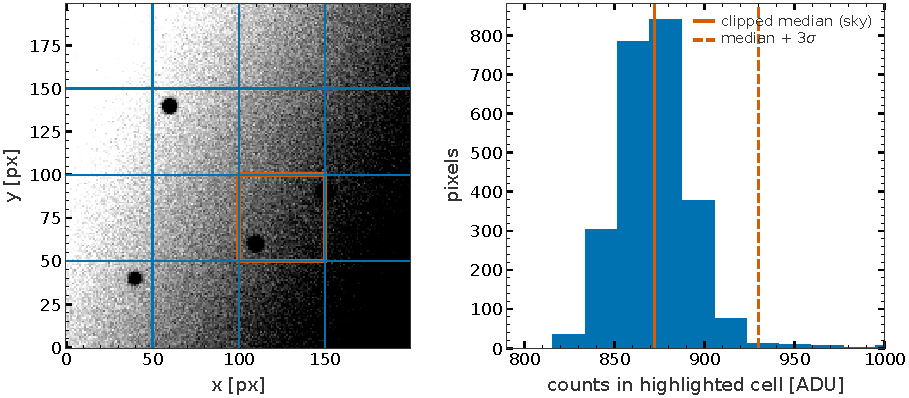
\includegraphics[width=\textwidth]{figures/fig_background.pdf}
\caption{Left: a toy frame (smooth gradient, noise, four sources) divided
into background meshes; one cell is highlighted. Right: the pixel
histogram of that cell. The sky is the narrow Gaussian body; the
sources contribute only the bright tail past the $3\sigma$ clip.}
\label{fig:toy_background}
\end{figure}

\lstinputlisting[language=Python]{examples/background_mesh.py}

%======================================================================
\section{Aperture photometry}
\label{sec:aperture}
%======================================================================

\code{photometry/aperture.py::Aperture.measure} performs circular-aperture
photometry on every source. The aperture radius is the per-image
\code{photometry.aperture\_radius} when set, else the data-driven optimum
radius (below), else \code{aperture\_size\,$\times$\,FWHM} (default
$1.7\times$FWHM), floored at \code{min\_aperture\_radius\_fwhm} on
undersampled data. Local sky is the sigma-clipped median of an annulus
separated from the aperture by \code{annulus\_gap\_fwhm} and of width
\code{annulus\_width\_fwhm} (crowded fields use tighter defaults); if the
annulus holds fewer than \code{annulus\_min\_pixels} usable pixels it is
widened.

\textbf{Flux and magnitude convention.} The integrated counts in
electrons within the aperture are $F_{\rm ap}$, and
$\mathrm{flux\_AP}=F_{\rm ap}/t_{\rm exp}$ in e$^-$~s$^{-1}$; magnitudes
are $m=-2.5\log_{10}(\mathrm{flux})$. The same rate convention applies to
PSF fluxes.

\textbf{Noise model.} The propagated variance sums the source Poisson
term and the sky term over the effective (fractional-pixel) aperture area
$A_{\rm eff}$, preferring photutils' \code{aperture\_sum\_err} evaluated
on the error map, with an annulus-estimator term added in quadrature
\citep{stetson1987daophot}:
\begin{equation}
\sigma_F^2 \;=\; \underbrace{F_{\rm src}}_{\rm source}
\;+\; \underbrace{A_{\rm eff}\,\max\!\big(\sigma_{\rm ann}^2,\,R^2\big)}_{\rm sky+read\;noise}
\;+\; \underbrace{\left(1.2533\,\frac{\sigma_{\rm ann}}{\sqrt{N_{\rm ann}}}\,A_{\rm eff}\right)^{2}}_{\rm annulus\ estimator},
\end{equation}
where $R$ is the read noise, $\sigma_{\rm ann}$ the MAD-scaled scatter of
the clipped annulus, and $N_{\rm ann}$ the usable annulus pixel count.
Resampling and template processing correlate pixel noise, so the
propagated variance is multiplied by an empirical noise factor $\eta$
(\code{empirical\_noise\_factor}): the ratio of measured empty-sky
aperture-sum scatter to the propagated prediction, measured on
$\sim$100 random sky apertures per image. It only inflates
($\eta\ge1$); $\eta>1.5$ additionally warns of confusion noise, and
per-image $\eta$ values are ledgered and summarised at driver level.
Magnitude errors use the linear approximation
\begin{equation}
\sigma_m = \frac{2.5}{\ln 10}\frac{\sigma_F}{F} = \frac{1.0857}{\mathrm{S/N}},
\end{equation}
consistent between AP and PSF outputs.

\textbf{Optimum radius.} \code{measure\_optimum\_radius} selects the
aperture from the curve of growth (CoG; \citealp{stetson1990growth}) of
isolated stars: per-source SNR-optimal radii \citep{howell1989snr} are
combined into a sigma-clipped median after a
concentration gate on the enclosed-flux fraction inside
$1.7\times$FWHM and a tail-stability screen
(\code{optimum\_radius\_*}), with a minimum kept-source count before the
estimate is trusted (\code{optimum\_radius\_min\_keep\_*}).

\textbf{Aperture correction.} \code{compute\_aperture\_correction}
measures the offset between the adopted aperture and the CoG total on
bright isolated stars (stored as \code{aperture\_correction} and its
error). The correction is embedded in the zero-point rather than applied
to individual fluxes: ZP$_{\rm AP}$ is fitted on raw \code{flux\_AP} and
therefore already contains the aperture loss, while the measured
correction is stored for the AP/PSF scale cross-check of
Section~\ref{sec:zeropoint}.

The mechanism is small enough to fit in a snippet
(Figure~\ref{fig:toy_aperture}): the net flux is the aperture sum minus
the annulus sky per pixel times the aperture area, and the S/N peaks at
an intermediate radius -- too small an aperture throws away signal, too
large an aperture admits more sky noise than signal.

\begin{figure}[ht]
\centering
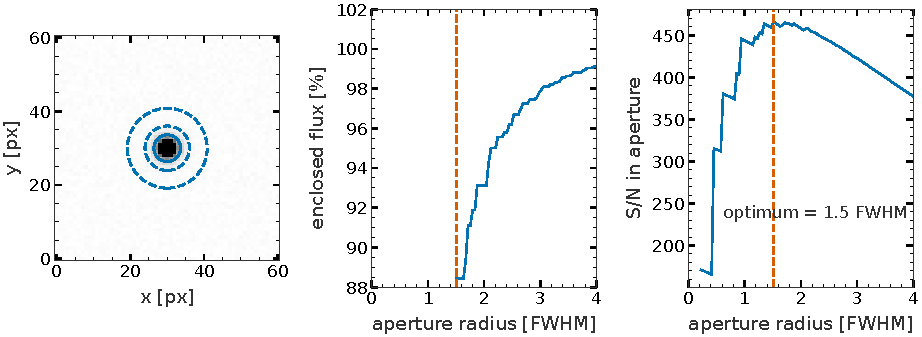
\includegraphics[width=\textwidth]{figures/fig_aperture.pdf}
\caption{Left: the source aperture (solid) and the sky annulus (dashed).
Centre: the curve of growth of a Moffat-profile star. Right: the
aperture S/N, which peaks at $\approx1.5$~FWHM -- the per-image optimum
the pipeline derives from its own stars (its default is
$1.7\times$FWHM).}
\label{fig:toy_aperture}
\end{figure}

\lstinputlisting[language=Python]{examples/aperture_photometry.py}

%======================================================================
\section{Empirical PSF construction}
\label{sec:epsf}
%======================================================================

\code{photometry/psf.py::PSF.build} constructs the point-spread model in
three tiers: a vetted empirical ePSF through photutils'
\code{EPSFBuilder} \citep{bradley2022photutils,anderson2000epsf}, a fitted
composite-Moffat analytic model \citep{moffat1969} used as build seed and
as fallback, and
an optional spatially varying \code{GriddedPSFModel}.

\subsection{Candidate pool and vetoes}

PSF stars are drawn from the detection catalogues and must clear an
extensive battery of cuts, each with keep-floor logic so that sparse
fields never end up with an empty pool
(\code{psf\_min\_candidates}, \code{psf\_pool\_preferred\_min}):

\begin{itemize}[leftmargin=1.6em,itemsep=0.5pt]
\item \emph{Catalogue level:} S/N bounds
  (\code{psf\_snr\_min/hard\_min/rescue\_min}, \code{psf\_threshold\_*}),
  saturation margin (\code{psf\_saturate\_fraction}), elongation
  (\code{psf\_elongation\_max}), SExtractor flags
  (\code{psf\_flags\_max}), isolation
  (\code{psf\_isolation\_radius\_fwhm}, neighbour S/N floor), pairwise
  blend/dedup checks (\code{psf\_min\_pair\_separation\_fwhm},
  \code{psf\_dup\_radius\_px}), profile-shape cuts in FWHM,
  \code{FLUX\_RADIUS}, \code{A\_}\slash\code{B\_IMAGE}, sharpness, and
  peak-to-aperture ratio, proximity to masked or defect pixels
  (\code{psf\_mask\_core\_min\_dist\_fwhm},
  \code{psf\_defect\_exclusion\_fwhm}, \code{psf\_spike\_*}), and a
  defect-dominance diagnostic. A candidate failing
  \code{psf\_defect\_veto\_min\_fails} independent cuts is removed
  unconditionally.
\item \emph{Ensemble level:} an FFT power-spectrum outlier test
  (\code{psf\_fft\_*}, relaxed on undersampled data where subpixel phase
  jitter dominates high-frequency power), and a flux-normalised
  shape-outlier test against the median stack
  (\code{psf\_shape\_outlier\_*}).
\item \emph{Cutout level} (\code{psf\_contam\_*}): quadrant-asymmetry,
  edge-ring and border excess, radial-profile reversal, secondary-peak
  detection in the core, row/column/diagonal streak medians,
  annulus local-maxima, total annulus flux excess, core ellipticity from
  second moments, a hot-pixel concentration test, and a normalised
  curve-of-growth test against both the clean-star ensemble and a Moffat
  encircled-energy envelope. Unrepairable classes (core secondary peaks,
  growth-curve failures, near-core masked pixels) are always rejected;
  when the keep-floor binds, contaminated annulus pixels are masked in
  place (\code{psf\_contam\_mask\_ring\_sigma}) and the star is kept.
\end{itemize}

\subsection{ePSF build}

Surviving cutouts (half-size $\ge$
\code{psf\_cutout\_size\_scale\_fwhm}$\times$FWHM, enclosing
\code{psf\_cutout\_ee\_fraction} of the flux) are flux-normalised inside
the aperture radius and passed to \code{EPSFBuilder}. Key behaviours:

\begin{itemize}[leftmargin=1.6em,itemsep=0.5pt]
\item \textbf{Oversampling.} \code{psf\_oversample} fixes the factor;
  \code{psf\_auto\_oversample\_undersampled} adapts it to the sampling
  and star count so that each oversampled gridpoint keeps
  $\ge$ \code{psf\_oversample\_min\_samples\_per\_pixel} star samples,
  bounded by \code{psf\_oversample\_max}.
\item \textbf{Smoothing.} The Anderson \& King quartic kernel
  (\code{psf\_smoothing\_kernel: quartic}, with a quadratic basis for
  $<5\times5$ footprints, or \code{auto}\slash\code{gaussian}\slash\code{none}) is
  sized from the native-pixel scale
  \code{psf\_smoothing\_kernel\_size\_scale\_px}, boosted when the
  effective samples per gridpoint fall below
  \code{psf\_smoothing\_kernel\_target\_samples}, and capped by
  \code{psf\_smoothing\_kernel\_max\_fwhm\_frac}$\times$FWHM.
\item \textbf{Iteration.} Adaptive iterations
  (\code{psf\_adaptive\_iterations}) start at
  \code{psf\_maxiters\_initial} and retry to \code{psf\_maxiters\_max};
  the per-star centre accuracy is relaxed on undersampled frames
  (\code{psf\_center\_accuracy\_undersampled} $\approx0.05$~px) where the
  default $10^{-3}$~px is unreachable and continued iteration walks the
  ePSF core narrow. Stars that fail to settle are pruned across
  \code{psf\_prune\_unsettled\_rounds} rounds; unsettled centroids are
  capped at \code{psf\_epsf\_max\_star\_shift\_px}.
\item \textbf{Seed and fallback.} A composite-Moffat model
  (\code{psf\_analytic\_components} core/mid/halo terms, optional shared
  centre offsets chosen by BIC) is fitted jointly over all star cutouts
  and used as the ePSF seed and residual diagnostic; when too few vetted
  stars reach the build (\code{psf\_build\_min\_stars}) or the empirical
  model fails its quality gates, the analytic composite (or a canonical
  Moffat built from the image FWHM alone) is delivered instead and the
  model is flagged \code{analytic-composite}\slash\code{analytic-canonical} in
  the output.
\item \textbf{Post-build gates.} The delivered ePSF's own FWHM must lie
  within $[0.85, 1.5]\times$ the image FWHM
  (\code{psf\_epsf\_fwhm\_min/max\_frac}), its negative-pixel fraction
  below \code{psf\_epsf\_negfrac\_max}, and its residuals against the
  star ensemble below \code{psf\_epsf\_residual\_ratio\_max}
  (\code{psf\_epsf\_residual\_gate}); failures fall back to the analytic
  model or to aperture-only photometry.
\end{itemize}

\subsection{Spatially varying models}
\label{sec:gridpsf}

With \code{psf\_spatial\_grid} (\code{auto}, or an integer $N$), the field
is split into detector grid cells (starved cells are grown into or merged
with neighbours, bounded by \code{psf\_grid\_max\_cells}), each cell runs
the full vetting/build pipeline with $\ge$
\code{psf\_grid\_min\_stars\_per\_cell} candidates, and the per-cell
stamps are combined into a \code{GriddedPSFModel}. Cell stamps must pass
per-cell FWHM, negative-fraction, and ensemble-consistency gates
(\code{psf\_grid\_cell\_*}); failed cells are filled from the nearest
populated neighbour or the whole grid is rejected
(\code{psf\_spatial\_fill\_missing}). With
\code{psf\_grid\_target\_aware}, cell boundaries are chosen to place the
target at the centre of its own populated cell, and
\code{psf\_grid\_require\_target\_cell} demands a real build there. A
shared oversampling factor is picked for the whole grid and can descend
when too few cells build (\code{psf\_grid\_osamp\_descent}).

The reason an empirical model is needed at all is visible in
Figure~\ref{fig:toy_epsf}: on the detector's native pixels a star is a
handful of noisy squares, but stars land at different sub-pixel phases,
so stacking many of them on a finer grid recovers the smooth
profile -- that stacked model is the ePSF.

\begin{figure}[ht]
\centering
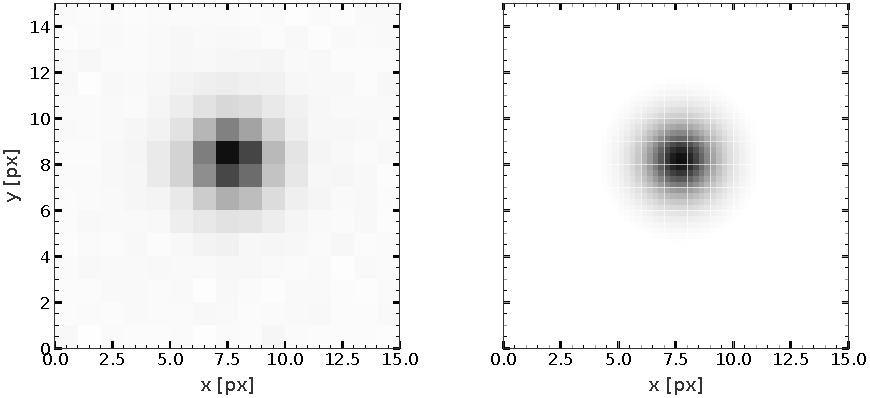
\includegraphics[width=\textwidth]{figures/fig_epsf.pdf}
\caption{Left: one star on the native pixel grid. Right: the same
profile on a grid four times finer (the white lines mark the native
pixel boundaries) -- the super-resolution the ePSF build recovers by
stacking cutouts at different sub-pixel phases.}
\label{fig:toy_epsf}
\end{figure}

\lstinputlisting[language=Python]{examples/epsf_oversampling.py}

%======================================================================
\section{PSF photometry}
\label{sec:psfphot}
%======================================================================

\code{photometry/psf.py::PSF.fit} fits the delivered model to all sources
with \code{photutils.PSFPhotometry}: cutouts are grouped when sources lie
within \code{psf\_group\_separation\_fwhm} of one another, fitted
simultaneously so blends are self-consistent, and the target is always
grouped with \code{additional\_targets} for the same reason. A constant
local background is estimated per group (the LPI option of
Section~\ref{sec:targetphot} replaces it with a regression infill under
the target). All sources share one fit box scaled from
\code{psf\_fit\_shape\_bright\_scale\_fwhm} with undersampled boosts, and
the fitted amplitude is bounded $\ge0$ on direct frames
(\code{psf\_fit\_positive\_flux}); on difference images
(\code{psf\_diff\_negative\_flux}) signed amplitudes can be kept for
fading sources.

\textbf{Centroid windows} make the target fit adaptive between free and
forced photometry. Below \code{fitting\_xy\_bounds\_detect\_snr}
(default S/N$=4$) the target's centroid is held within
\code{fitting\_xy\_bounds\_hold\_px} of the catalogue seed (widened by the
measured astrometric uncertainty when
\code{fitting\_xy\_bounds\_astrometric}), i.e.\ the measurement degrades
gracefully to forced photometry. The in-window detection S/N is an
aperture statistic measured on the image: flux inside
\code{aperture\_radius} at the peak found within the search disk, minus
the median of window pixels outside that disk, over an aperture-sum
noise of local \code{background\_rms} scaled by
$\sqrt{A + (1.2533\,A)^{2}/N_{\rm sky}}$ -- the same pixel-plus-annulus
budget as aperture photometry -- multiplied by the empirical noise
factor $\eta$ to cover resampled-pixel correlation. A bright peak found
beyond $\sim$0.5\,FWHM of the seed is treated as a neighbour rather
than the target, and its Gaussian wing contribution is subtracted from
the seed aperture before the S/N is evaluated. Between that floor and
\code{fitting\_xy\_bounds\_full\_snr} the bound grows linearly to the
free window (\code{fitting\_xy\_bounds} arcsec, additionally floored and
capped by \code{fitting\_xy\_bounds\_target\_*}). A fit that latches onto
the bound edge (\code{fitting\_xy\_bounds\_edge\_frac}) is refit held at
the seed so the reported flux cannot belong to a neighbour;
\code{force\_photometry} pins every target regardless of S/N.

\textbf{Fitters.} Three engines are available. The default is bounded
Levenberg-Marquardt least squares. \code{use\_poisson\_likelihood\_fitter}
selects a Poisson maximum-likelihood fit (step-projected to honour the
positive-flux bound, \code{poisson\_*}). Above
\code{perform\_emcee\_fitting\_s2n} (S/N$>10$ by default) the LSQ solution
is refined by an affine-invariant MCMC \citep{foreman2013emcee} that
samples position, flux, and local sky with proper uncertainty
propagation, using \code{emcee\_nwalkers}, adaptive length
(\code{emcee\_adaptive\_tau\_target}, \code{emcee\_early\_stop}), burn-in
fraction, thinning, and convergence diagnostics that feed the quality
flags. Reported flux errors carry the fit covariance inflated by
$\sqrt{\chi^2_{\rm red}}$ where appropriate, plus the SFFT kernel-model
term of Section~\ref{sec:subtraction}.

\textbf{Detection statistic.} Alongside photometry, the code evaluates a
matched-filter probability \citep{zackay2016proper}: for the
PSF-plus-sky model $H_1$ against the sky-only model $H_0$ in a box around
the fitted position,
\begin{equation}
a=\frac{\sum_i w_i p_i d_i}{\sum_i w_i p_i^2},\qquad
z=a\sqrt{\sum_i w_i p_i^2},\qquad
\mathrm{prob\_detect}=\Phi\!\left(\frac{z}{\kappa}\right),
\end{equation}
with $w_i=1/\sigma_i^2$, $p_i$ the unit-flux ePSF, and
$\kappa=\mathrm{clip}(\sqrt{\chi^2_{\rm red}},1,10)$. The statistic is
signed (oversubtraction dips drive prob$\to0$) and is suppressed when a
narrower, broader, or dipole-shaped template fits the box better than the
PSF. It feeds both the detection rescue of
Section~\ref{sec:detection} and the empirical false-alarm veto, which
evaluates the same statistic at $\sim$60 blank annulus sites
(3--8$\times$FWHM) around the target.

%======================================================================
\section{Reference catalogues and photometric systems}
\label{sec:catalog}
%======================================================================

\code{calibration/catalog.py::Catalog} downloads the field sequence once
per (catalogue, band, footprint region) via \code{build\_complete\_catalog},
querying through \code{astroquery} \citep{ginsburg2019astroquery},
including VizieR \citep{ochsenbein2000vizier},
and serves it to every image of the run. Supported backends:
\code{gaia} (Gaia DR3, including synthetic photometry from XP spectra via
GaiaXPy \citep{weiler2023gaiaxpy} and SVO filter transmission curves
\citep{rodrigo2012svo,gaia2023dr3}), \code{refcat} (ATLAS Refcat2;
\citealp{tonry2018refcat}), \code{pan\_starrs}\slash\code{panstarrs}
(Pan-STARRS1 DR2 mean; \citealp{chambers2016panstarrs,tonry2012ps1}),
\code{sdss} \citep{york2000sdss}, \code{apass}
\citep{henden2016apass}, \code{2mass} \citep{skrutskie2006twomass},
\code{legacy} (DESI Legacy Imaging Surveys; \citealp{dey2019legacy}),
\code{skymapper} \citep{wolf2018skymapper}, and \code{custom} (user CSV;
\code{catalog\_custom\_fpath}). Query geometry follows the image
footprint rather than a blind cone around the target
(\code{region\_*}), with coverage-aware recentering when the catalogue
does not fill the frame (\code{coverage\_recenter\_min}).

Catalogue rows are cleaned before calibration: magnitude range
(\code{zeropoint.faint\_mag\_limit}, \code{bright\_mag\_limit}),
saturation/nonlinearity against the image's own linearity curve
(\code{reject\_nonlinear\_sources}, \code{nonlinear\_peak\_frac},
\code{saturation\_peak\_frac}), SExtractor flags
(\code{zeropoint.max\_flags}), FWHM-outlier and defect rejection, blends
(\code{blend\_neighbor\_*}), star-galaxy separation on catalogue Kron
magnitudes \citep{kron1980} where the backend provides them,
known-variable matching, and a minimum
surviving count (\code{min\_source\_no}, \code{clean\_min\_keep}).

\textbf{Photometric systems.} Band names are case-significant
(Section~\ref{sec:ingestion}); the catalogue column map is
\code{autophot/data/catalog.yml} and the default colour pair per band is
\code{filters.yml:default\_dmag}. When a catalogue does not natively
carry the image band, published transformations can synthesize it
(\code{catalog.allow\_filter\_transformations}): SDSS$ugriz\to UBVRI$
\citep{lupton2005sdss,jester2005}, PS1$\to$ Johnson-Cousins $BVRI$
\citep{tonry2012ps1}, Legacy Survey natural-system inversions
\citep{legacydr10}, and DECaLS/MzLS$+$BASS$\to$SDSS piecewise relations
\citep{toptun2024}. Each transformation's published scatter is folded
into the synthesised magnitude error so transformed calibrators are
weighted correctly. \code{include\_IR\_sequence\_data} adds 2MASS $JHK$
calibrators to optical fits.

%======================================================================
\section{Photometric calibration (zero-point)}
\label{sec:zeropoint}
%======================================================================

\code{calibration/zeropoint.py::Zeropoint} fits, separately for the
aperture and the PSF measurements of each matched calibrator,
\begin{equation}
\Delta m_i \;=\; m_{{\rm cat},i}-m_{{\rm inst},i}
\;=\; \mathrm{ZP}+\sum_{k=1}^{n} c_k\,(C_{1,i}-C_{2,i})^{k}
\end{equation}
(polynomial orders $n=1,2$ via \code{color\_term\_poly\_order}, or a
piecewise-linear form with \code{color\_term\_n\_segments}$>1$ segments
and a fitted break), where $C_{1}-C_{2}$ is the default colour for the
band from \code{filters.yml}. Zero-points are fitted on raw instrumental
magnitudes, so the aperture ZP embeds the aperture correction; a pure
intercept (no colour term) is fitted when
\code{apply\_colorterms: false} or colour data are missing.

\textbf{Fit methods} (\code{zeropoint.fit\_method}): \code{mcmc} (the
default; affine-invariant sampling of the locus with errors in both
coordinates, \code{mcmc\_n\_walkers/burn/steps} with an autocorrelation
stop at \code{mcmc\_tau\_factor}), \code{odr} (orthogonal distance
regression; \citealp{boggs1987odr}), and \code{ransac} (robust inlier
search; \citealp{fischler1981ransac}). Calibrator
outliers are rejected by iterative sigma clipping capped at
\code{sigma\_clip\_max} seeded at a robust mode; a fast path accepts a
clean fit early (\code{fast\_path\_max\_mad}); a PSF-vs-AP disagreement
gate (\code{ap\_psf\_disagree\_min\_mag}) and a minimum inlier fraction
(\code{min\_inlier\_fraction}, \code{max\_inlier\_mad}) guard against
systematic loci.

\textbf{Extensions.} An optional spatial ZP surface
(\code{spatial\_zp\_surface}: low-order polynomial in detector
coordinates adopted only on a significant F-test improvement and bounded
by \code{max\_correction\_mag}) models vignetting/illumination
residuals, and a magnitude-dependent diagnostic
(\code{magnitude\_dependent\_zp}) bins the residual locus to flag
nonlinear response beyond \code{max\_zp\_trend\_mag}.

\textbf{Zero-point error model.} The reported
\code{zeropoint\_error} combines in quadrature the statistical error on
the mean (formal weighted error inflated by $\chi^2/\mathrm{dof}$ when
residuals exceed claimed errors, floored at the standard error of the
inlier median) and \code{zeropoint.systematic\_err} (default $0.02$~mag)
for field-correlated calibration systematics;
\code{zeropoint\_scatter} reports the robust dispersion
$\mathrm{MAD}\times1.4826$ of the inlier locus and
\code{zeropoint\_error\_stat} the pre-systematic component. Bootstrap
resampling (\code{bootstrap\_resamples}) provides the sampling
distribution. When a spatial surface is used, the effective number of
independent calibrators (\code{spatial\_corr\_min\_neff\_frac}) inflates
the error.

\textbf{Target magnitudes.} For each photometry channel,
$m_{\rm cal}=m_{\rm inst}+\mathrm{ZP}+c\,(C_{\rm target})$. When the
target has catalogue colours (a known variable) the actual colour term
applies; for a transient with unknown colour the median calibrator colour
is adopted and both $|c|\,\sigma_{\rm colour}$ and
$|c_{\rm err}|\,|\bar{C}|$ are added as systematics
(Section~\ref{sec:errors}).

At its simplest the fit is one number
(Figure~\ref{fig:toy_zeropoint}): the offset between catalogue and
instrumental magnitudes over the surviving calibrators, with the
handful of discrepant points clipped away first.

\begin{figure}[ht]
\centering
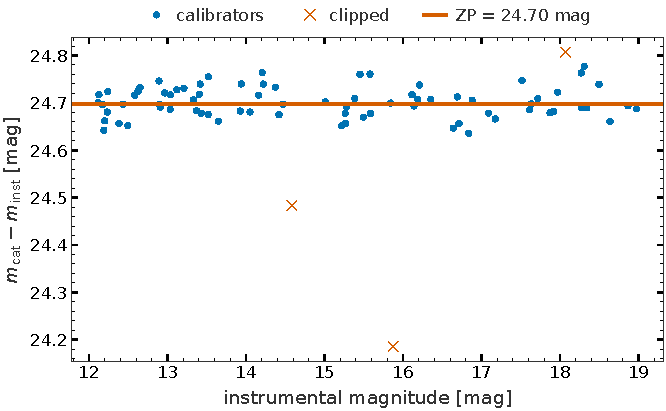
\includegraphics[width=0.74\textwidth]{figures/fig_zeropoint.pdf}
\caption{Catalogue minus instrumental magnitude versus instrumental
magnitude for toy calibrators. The flat locus is the zero point; the
marked outliers are what iterative sigma clipping removes before the
offset is taken.}
\label{fig:toy_zeropoint}
\end{figure}

\lstinputlisting[language=Python]{examples/zeropoint_fit.py}

%======================================================================
\section{Template subtraction}
\label{sec:subtraction}
%======================================================================

With \code{template\_subtraction.do\_subtraction: true},
\code{subtraction/templates.py::Templates} locates the band-matched
reference (local \code{templates/} directory or downloaded survey
cutout), aligns it, flux-matches it, and subtracts it.

\subsection{Alignment cascade}

\code{Templates.align} tries a per-method cascade; the first method to
pass the quality gates wins:

\begin{center}
\small
\begin{tabular}{@{}ll@{}}
\toprule
Requested & Cascade order \\
\midrule
\code{spalipy} & spalipy $\to$ SCAMP$+$SWarp $\to$ WCS reproject $\to$ AstroAlign \\
\code{swarp} & SCAMP$+$SWarp $\to$ reproject $\to$ AstroAlign \\
\code{reproject} & reproject $\to$ AstroAlign $\to$ SCAMP$+$SWarp \\
\code{astroalign} & AstroAlign $\to$ reproject $\to$ SCAMP$+$SWarp \\
\code{tweakwcs} & tweakwcs $\to$ SCAMP$+$SWarp $\to$ reproject $\to$ AstroAlign \\
\code{chi2\_shift} & chi2\_shift $\to$ SCAMP$+$SWarp $\to$ reproject $\to$ AstroAlign \\
\bottomrule
\end{tabular}
\end{center}

spalipy performs quad-hash geometric matching and spline-warp resampling
\citep{spalipy}; SCAMP$+$SWarp refits the template WCS against Gaia and
resamples with \code{reproject}-family interpolation
\citep{bertin2006scamp,bertin2010swarp,robitaille2020reproject};
\code{tweakwcs} adjusts the WCS directly from matched sources
\citep{tweakwcs}; \code{chi2\_shift} cross-correlates for extended fields
\citep{guizar2008efficient}; AstroAlign matches source triangles
\citep{beroiz2020astroalign}. Quality gates require
\code{alignment\_min\_matched\_sources} matches and bound the matched
offset RMS, 90th-percentile, and the local offset near the target
(\code{alignment\_max\_rms\_px}, \code{alignment\_max\_p90\_px},
\code{alignment\_target\_*}); a post-SWarp verification pass and
per-attempt metrics (\code{Alignment\_<base>.json}) record which cascade
step produced the accepted alignment.

\subsection{Flux matching}

A scale factor FSCALE is derived from pipeline-vetted sources common to
both frames (the flux-consistent subset selected by
\code{find\_flux\_consistent\_sources} after S/N, morphology, defect,
isolation, and stamp-level cuts, with the target region excluded). The
difference image therefore inherits the science frame's photometric
scale, and the ratio $f=\mathrm{FSCALE}_{\rm obs}/\mathrm{FSCALE}_{\rm exp}$
is propagated as a flux-scale systematic
(\code{photometry.detection\_*}, \code{sfft\_fscal\_*} guards).

\subsection{Subtraction backends}

\code{Templates.subtract} runs one of three backends
(\code{template\_subtraction.method}, with \code{auto} choosing by FWHM
match):

\begin{itemize}[leftmargin=1.6em,itemsep=1pt]
\item \textbf{SFFT} \citep{hu2022sfft,russell2022sfft} (default,
  \code{sfft}): the matching kernel $K$ in
  $\mathrm{SCI}=\mathrm{REF}\otimes K$ is solved in a delta-function
  (or B-spline) basis \citep{alard1998method} over stamp regions centred
  on the vetted kernel
  prior sources, via the \code{Easy\_SparsePacket}\slash\code{Easy\_CrowdedPacket}
  APIs in a \code{run\_sfft.py} subprocess (numpy or CUDA backend,
  \code{sfft\_backend}, \code{sfft\_num\_threads}). The convolution
  direction follows \code{forceconv}: \code{REF} (default; convolve the
  template to the science PSF, preserving science-frame photometry),
  \code{SCI}, or \code{AUTO} within
  \code{sfft\_forceconv\_auto\_tol}, and deconvolution can be vetoed
  (\code{sfft\_veto\_deconvolution}). Kernel order
  (\code{kernel\_order}), half-width sizing
  (\code{kernel\_hw\_*} or \code{sfft\_auto\_kernel\_size}),
  regularisation (\code{sfft\_regularize\_*}), crowded-mode parameters
  (\code{sfft\_crowded\_*}, \code{sfft\_bg\_order},
  \code{sfft\_const\_phot\_ratio}), and prior-source vetoes
  (\code{sfft\_psf\_*}, \code{sfft\_flux\_linearity\_*},
  \code{sfft\_max\_*}) are configurable; kernel anomalies trigger a retry
  ladder (noise, negative fraction, spatial order) and post-subtraction
  checks feed back into the source list
  (\code{sfft\_use\_post\_anomaly\_feedback}).
\item \textbf{HOTPANTS} \citep{becker2015hotpants}: external executable
  (\code{hotpants\_exe\_loc}, \code{hotpants\_timeout}), stamp selection
  from the same vetted sources, external noise maps via \code{-ini/-tni}.
\item \textbf{ZOGY} \citep{zackay2016proper}: a self-contained numpy
  implementation with per-pixel noise maps
  (\code{zogy\_per\_pixel\_noise}, box-estimated
  \code{zogy\_noise\_map\_box\_size}), an optional least-squares kernel
  refinement over stamp sources (\code{zogy\_lsq\_*}), a residual
  astrometric-shift search and small warp correction
  (\code{zogy\_astrometric\_shift}, \code{zogy\_residual\_warp}), an
  astrometric noise floor (\code{zogy\_astrometric\_noise\_floor\_px}),
  adaptive Wiener filtering, score-image output
  (\code{zogy\_write\_score\_images}), and NaN filling.
\end{itemize}

\subsection{Difference-image quality}

Post-subtraction checks include the flux-scale discrepancy
(\code{sfft\_fscal\_phot\_sanity\_frac}, aperture-level cross-checks),
static-source residual statistics, and a residual-artifact masker that
locates PSF-mismatch dipoles (positive/negative lobe pairs) and masks
them for subsequent photometry (\code{residual\_artifact\_*}). The
difference header records \code{CONVD}\slash\code{FORCECON} so downstream code
knows which frame was convolved (this matters for the correct PSF to fit
on the difference image). The SFFT kernel's spatial model contributes a
fractional flux error folded into PSF photometry
(\code{psf\_kernel\_model\_err\_frac}), and the difference image carries
$\mathrm{Var}\approx\sigma_{\rm sci}^2+\sigma_{\rm tpl}^2$ noise.

The end result is the familiar three-panel picture of
Figure~\ref{fig:toy_subtraction}: once the template is aligned,
flux-matched, and PSF-matched, the difference carries only what
changed.

\begin{figure}[ht]
\centering
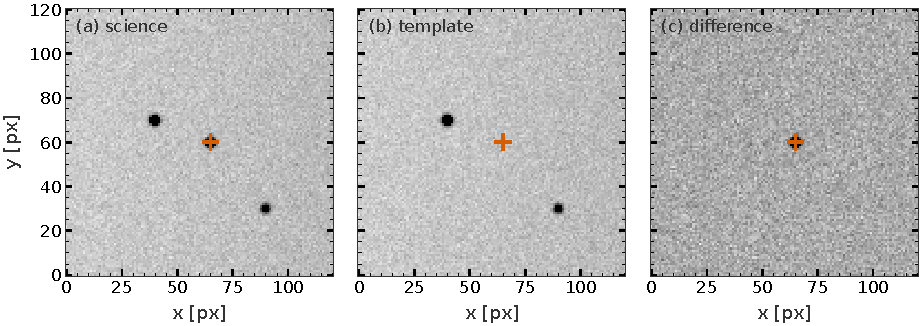
\includegraphics[width=\textwidth]{figures/fig_subtraction.pdf}
\caption{Toy subtraction. (a) Science frame: sky, two static sources,
and a transient (marked). (b) The aligned template. (c) The difference
image: sky and static sources cancel, leaving the transient's PSF --
and doubled pixel noise.}
\label{fig:toy_subtraction}
\end{figure}

\lstinputlisting[language=Python]{examples/template_subtraction.py}

%======================================================================
\section{Target photometry and detection}
\label{sec:targetphot}
\label{sec:detection}
%======================================================================

Aperture and PSF photometry run at the target's catalogue position on
both the direct and the difference image. The target PSF fit shares the
field fit's conventions (Section~\ref{sec:psfphot}) with the adaptive
centroid windows described there; \code{check\_inverted\_image} repeats
the fit on the sign-flipped difference image to measure transients that
faded below the template. An optional LPI-style local background infill
(\code{lpi\_background\_for\_target} and the \code{lpi\_*} parameters, in
development) replaces the annulus estimate under the target with a
ridge-regression prediction conditioned on shifted samples of the
surrounding sky, tolerating structured host-galaxy backgrounds.

\subsection{Detection decision}
\label{sec:detgates}

\code{main.py::\_decide\_detection} combines independent gates; a
measurement is reported as a detection only when it survives all
applicable ones:

\begin{enumerate}[leftmargin=2em,itemsep=0.5pt]
\item \textbf{S/N} $\ge$ \code{detection\_limit} (default 3; the
forced-photometry SNT convention).
\item \textbf{Positive flux} in the primary channel (catches
oversubtraction dips; inverted fits reverse the sign convention).
\item \textbf{Fit quality}: reduced $\chi^2\le$
\code{detection\_max\_chi2} for the PSF channel.
\item \textbf{AP/PSF sign consistency}
(\code{detection\_flux\_consistency}): opposite signs flag a
subtraction artifact.
\item \textbf{Centroid veto}: the fitted position must lie within
\code{detection\_max\_offset\_arcsec} of the target (larger offsets mean
the fit locked onto a neighbour or artifact).
\item \textbf{Empirical FAP veto}: \code{prob\_detect} is evaluated at
\code{detection\_empirical\_trials} blank annulus sites (3--8$\times$FWHM)
on the same image; if the fraction reaching the target's value exceeds
\code{detection\_empirical\_max\_pfalse} (and S/N $<$
\code{detection\_empirical\_snr\_max}), the point is rejected as a
correlated-noise fluctuation.
\end{enumerate}

Two rescue channels counter false rejections: an aperture-SNR fallback
(\code{detection\_ap\_fallback\_ratio}$\times$ threshold, AP being less
sensitive to PSF-model mismatch on faint sources) and a matched-filter
rescue (\code{detection\_mf\_snr\_min} with
\code{prob\_detect}$\ge$\code{detection\_mf\_prob\_min} and positive flux;
the empirical-FAP and centroid vetoes still apply). Non-detections report
an upper limit at the second entry of
\code{limiting\_magnitude.snr\_thresholds} (SNU convention, default 5):
the multi-threshold limiting magnitude machinery of
Section~\ref{sec:limits} when available, else the 50\%-completeness
limit. Every epoch also carries the \code{quality\_flags} bitmask
(Section~\ref{sec:outputs}).

%======================================================================
\section{Limiting magnitudes}
\label{sec:limits}
%======================================================================

\code{analysis/limits.py::Limits.get\_injected\_limits\_multi\_snr}
estimates local depth empirically. ePSF-shaped sources of known
instrumental magnitude are injected at \code{injection\_n\_sites} random
positions in an annulus around the target
(\code{inject\_min\_radius\_fwhm} to \code{inject\_max\_radius\_fwhm};
sites avoid neighbours, bright wings, zero/variance-poor pixels, and
non-finite annuli through the \code{inject\_*} gates, and each site is
repeated with subpixel jitter \code{injection\_jitter\_pix}$\times$
\code{injection\_jitter\_repetitions}). Poisson noise can be added
(\code{inject\_source\_poisson\_noise}). Recovery then applies the
\emph{same} photometry path and criteria as the real target
(\code{recovery\_method: auto}), so the completeness estimate inherits
the pipeline's own systematics.

For each threshold in \code{snr\_thresholds} (default $[3,5]$), the
recovery fraction as a function of magnitude is fitted with the logistic
\begin{equation}
P(\mathrm{det}\mid m)=\frac{1}{1+\exp\!\big((m-m_{50})/s\big)},\quad s>0,
\end{equation}
sampled with emcee (\code{logistic\_emcee\_*}) to give the
completeness curve, the $m_{50}$ point, and the magnitude at each
S/N threshold; \code{completeness\_solver: bisect} provides a
non-MCMC alternative and \code{adaptive\_snr\_selection} chooses which
thresholds to report. A bootstrap (\code{m50\_bootstrap\_n}) distributes
$m_{50}$. Finally, an uncertainty calibration
(\code{uncal\_*}) compares the claimed S/N of recovered injections with
their measured scatter and rescales the reported errors when they
systematically under- or over-estimate the true noise
(\code{uncal\_apply}, clipped to \code{uncal\_factor\_clip}).

The recipe in miniature is Figure~\ref{fig:toy_limits}: injected
sources fade through the detection threshold, the recovered fraction
as a function of magnitude is the completeness curve, and its 50\%
point is the reported limit.

\begin{figure}[ht]
\centering
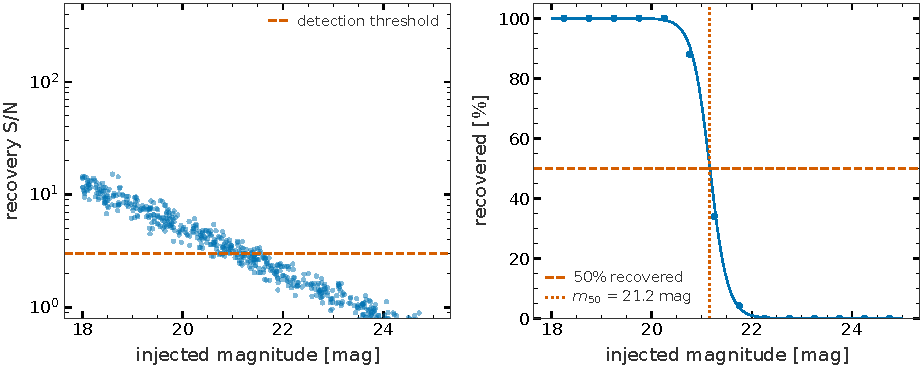
\includegraphics[width=\textwidth]{figures/fig_limiting.pdf}
\caption{Left: recovery S/N of injected toy sources versus their true
magnitude, with the detection threshold dashed. Right: the fraction
recovered per magnitude bin and the fitted logistic completeness
curve; the limit is the 50\% point, $m_{50}$.}
\label{fig:toy_limits}
\end{figure}

\lstinputlisting[language=Python]{examples/limiting_magnitude.py}

%======================================================================
\section{Host-galaxy modelling}
\label{sec:hostmodel}
%======================================================================

An optional host-surface-photometry stage
(\code{host\_model.enabled}) subtracts a smooth galaxy model before
photometry: SExtractor seeds feed a GALFIT run
\citep{peng2002galfit} (\code{engine: galfit},
\code{galfit\_path}) fitting \code{n\_sersic} S\'ersic components plus an
optional nuclear point source within \code{fit\_radius\_fwhm}, the target
position being held fixed or excluded from the model seeds
(\code{hold\_target\_position}, \code{seed\_exclude\_target\_fwhm}). The
residual frame then carries the transient on a flattened host. This
complements (and is distinct from) the LPI local infill of
Section~\ref{sec:targetphot}: GALFIT models the host globally, the LPI
infill models only the sky under the target's PSF.

%======================================================================
\section{Outputs and post-processing}
\label{sec:outputs}
%======================================================================

Per-image products land next to the science frame under
\code{outdir\_name}:

\begin{itemize}[leftmargin=1.6em,itemsep=1pt]
\item the science FITS with updated header (WCS, \code{FWHM},
\code{CONVD}\slash\code{FORCECON}, ZP keywords), the background model and the
\code{<base>.weight.fits} RMS map, the aligned template and the
difference image;
\item a per-image CSV with the target row: positions (catalogue seed and
fitted centroid), \code{flux\_ap/flux\_AP}, \code{flux\_psf/flux\_PSF} and
errors, S/N per channel, instrumental and calibrated magnitudes in the
image band, \code{reduced\_chi2}, \code{prob\_detect}, \code{mf\_snr},
empirical \code{p\_false}, detection flag, limiting magnitudes at each
threshold, the \code{psf\_model} used, and the \code{quality\_flags}
bitmask;
\item diagnostic plots (aperture curve of growth, ePSF build residuals,
ZP locus, alignment vector maps, injection-recovery completeness),
written as \code{plot\_format};
\item the per-image \code{LOG\_<base>.log} (full DEBUG) and
\code{Alignment\_<base>.json} metrics.
\end{itemize}

The \code{quality\_flags} integer combines per-epoch conditions
(Table~\ref{tab:qflags}); \code{is\_fatal()} and \code{is\_degraded()}
classify unusable versus cautionary measurements for light-curve
consumers.

\begin{table}[ht]
\centering\small
\caption{\code{quality\_flags} bitmask layout (\code{core/quality\_flags.py}).}
\label{tab:qflags}
\begin{tabular}{@{}ll@{}}
\toprule
Bit range & Flags \\
\midrule
0--4 & data: non-finite pixels, $>20\%$ masked, edge, saturated, bad background \\
8--12 & PSF: few stars, poor fit, spatial variation, undersampled, model mismatch \\
16--25 & fitting: low S/N, non-convergence (LSQ/MCMC), low ESS, at bound, \\
       & \hspace{1em} suspicious residuals, crowded, negative flux, MCMC fallback, degeneracy \\
26+ & pipeline: no/few-star zero-point, poor alignment \\
\bottomrule
\end{tabular}
\end{table}

At driver level the per-image rows are merged into a per-band
\code{<target>\_<band>.csv} light curve and plotted; an instrument column
(\code{lightcurve\_instrument\_column}, with
\code{lightcurve\_instrument\_aliases}) keeps mixed-facility epochs
distinguishable. Optional post-processing computes an inter-band
transient colour correction (\code{postprocessing.transient\_color\_correction}),
an RGB composite from the per-band products
(\code{color\_image}: asinh stretch with configurable softening,
percentile clipping, gamma), and a Lomb-Scargle periodogram
\citep{lomb1976,scargle1982} of the light curve
(\code{periodogram\_*}), in PSF or AP flavour.

The light-curve CSV is long-form (one row per image, a \code{filter}
column). The usual next steps are one-liners:

\begin{lstlisting}[language=Python]
from autophot.analysis.lightcurve import (
    plot_lightcurve, generate_photometry_table,
)
from autophot.photometry.differential_photometry import (
    differential_photometry,
)

plot_lightcurve(output_csv, snr_limit=3, method="PSF")  # detections + limits
generate_photometry_table(output_csv, snr_limit=3, method="PSF")  # ASCII table
differential_photometry(output_csv, method="PSF")      # vs reference ensemble
\end{lstlisting}

%======================================================================
\section{Error-budget summary}
\label{sec:errors}
%======================================================================

The reported magnitude error on a target epoch combines, in quadrature,
the terms in Table~\ref{tab:errors}. The convention
$\sigma_m=1.0857/(\mathrm{S/N})$ is uniform across aperture, PSF, and
limiting-magnitude outputs, and every term is quality-gated rather than
silently dropped: missing terms are absent only when the corresponding
stage did not run.

\begin{table}[ht]
\centering\small
\caption{Terms folded into the reported photometric error.}
\label{tab:errors}
\begin{tabular}{@{}lll@{}}
\toprule
Term & Origin & Configuration \\
\midrule
source Poisson $+$ sky $+$ read noise & aperture/PSF fit & header \code{GAIN}, \code{RDNOISE} \\
annulus estimator noise & local-sky subtraction & annulus sizing \\
resampling/noise correlation & empirical factor $\eta$ & \code{empirical\_noise\_factor} \\
PSF fit covariance & LSQ/MCMC posterior & fitter, $\chi^2$ inflation \\
SFFT kernel model & spatial kernel systematics & \code{psf\_kernel\_model\_err\_frac} \\
zero-point & stat $\oplus$ \code{systematic\_err} & \code{zeropoint.*} \\
colour term (transient) & median-colour assumption & \code{color\_scatter}, slope error \\
aperture correction & CoG total-vs-aperture & stored \code{aperture\_correction\_err} \\
systematic floor & flat-fielding, model error & \code{systematic\_error\_floor\_mag} \\
uncal rescaling & injection-derived calibration & \code{limiting\_magnitude.uncal\_*} \\
\bottomrule
\end{tabular}
\end{table}

%======================================================================
\section{Reproducibility and performance}
\label{sec:repro}
%======================================================================

\textbf{Determinism.} With \code{rng\_seed: null} each image derives its
seed from the file content, so identical inputs reproduce bit-identical
photometry; an integer forces a shared seed for every image. MCMC chains
use \code{emcee\_random\_state} and \code{zeropoint.random\_state}; the
pipeline pins BLAS/OpenMP to one thread before numerical imports so that
worker processes cannot oversubscribe.

\textbf{Parallelism.} \code{nCPU} controls image-level workers
(subprocesses with per-image logs); within an image,
\code{photometry.aperture\_n\_jobs}, \code{limiting\_magnitude.n\_jobs},
SExtractor/SCAMP \code{nthreads}, and \code{emcee\_threads} multiply it,
and the driver warns when the product exceeds the core count.
\code{nGPU} pins workers round-robin to visible devices (relevant to
\code{sfft\_backend: cupy}).

\textbf{Restart and caching.} \code{restart: true} reprocesses everything;
\code{false} reuses intermediate outputs (except
\code{photometry.redo\_sources}). \code{wdir} holds the telescope
database, catalogue caches (\code{gaia\_cache\_ttl\_days}), template
products, and the empirical-noise-factor ledger. External tool failures
are logged and quality-flagged rather than swallowed by broad exception
handlers; every stage writes to the per-image log regardless of console
verbosity.

%======================================================================
\appendix
\section{Configuration parameter reference}
\label{app:params}
%======================================================================

The tables below list every parameter in
\code{autophot/data/default\_input.yml}, grouped by configuration
section; the large \code{photometry} block is split into functional
sub-tables. Each entry shows the YAML key, its default and declared type,
and the description carried in the default file. Keys marked
\emph{(runtime)} are populated per image by the pipeline and exist in the
schema for typing; user overrides are ignored or overwritten. Keys marked
\emph{(deprecated)} are kept for backwards compatibility but no longer
affect the reduction (the replacement, where one exists, is named in the
description); keys marked \emph{(unreferenced)} have no consumer anywhere
in the package and are removal candidates (Section~\ref{sec:param-audit}).
The tables are generated by \code{scripts/generate\_parameter\_appendix.py} so they
track the file exactly; \code{autophot-main -{}-config-help} prints the
same map at the command line.

\subsection{Parameter usage audit}
\label{sec:param-audit}

Every leaf key in \code{default\_input.yml} was traced to a code
reference: \code{scripts/audit\_config\_usage.py} searches the package
source for each key name, and misses are checked by hand against dynamic
key construction (formatted names, \code{startswith} iteration, whole-dict
pass-through to external tools). The audit found twelve keys that were
either never read or read only as compatibility shims with no effect on
the result (Table~\ref{tab:dead-params}); they have been removed from the
schema and registered in
\code{functions.py::\_CONFIG\_REMOVED\_KEYS}, so user configs that still
carry them print a ``no longer used'' warning rather than an unknown-key
error. All 900 remaining leaf parameters are consumed directly.

\begin{table}[ht]
\centering\small
\begin{tabular}{@{}p{7.4cm}p{8.2cm}@{}}
\toprule
Key & Finding \\
\midrule
\code{wcs.code\_tolerance} & never read; no solver backend consumes it \\
\code{host\_model.engine} & no engine dispatch; only galfit exists \\
\code{template\_subtraction.alignment\_clustered\_span\_frac} &
  coherent-cluster gate hardcodes a 0.25 span \\
\code{template\_subtraction.alignment\_clustered\_quadrant\_frac} &
  same gate hardcodes ``$<$2 quadrants'' \\
\code{photometry.psf\_adaptive\_smoothing\_kernel} & deprecated no-op \\
\code{background.local\_interp\_order} & deprecated no-op (photutils\,$\ge$\,3) \\
\code{background.global\_interp\_order} & deprecated no-op (photutils\,$\ge$\,3) \\
\code{photometry.upper\_limit\_snr} & documented but never read; the
  \code{limiting\_magnitude.snr\_thresholds} list supplies the SNU
  convention \\
\code{photometry.apply\_aperture\_correction} & read only to log a note;
  \code{ZP\_AP} already embeds the aperture loss \\
\code{photometry.oversample\_psf\_fwhm} & read into a variable that was
  never used; \code{undersampled\_fwhm\_threshold} decides \\
\code{background.global\_interpolator} & logged and ignored
  (photutils\,$\ge$\,3 always uses cubic zoom) \\
\code{background.local\_interpolator} & logged and ignored
  (photutils\,$\ge$\,3 always uses cubic zoom) \\
\bottomrule
\end{tabular}
\caption{Former parameters of \code{default\_input.yml} with no consumer
in the current code; removed from the schema and listed in
\code{\_CONFIG\_REMOVED\_KEYS} for backwards-compatible handling of old
configurations.}
\label{tab:dead-params}
\end{table}

The two \code{alignment\_clustered\_*} keys describe thresholds that were
planned for the coherent-cluster gate in
\code{templates.py::compute\_alignment\_rms} (a sparse alignment whose
matched anchors bunch into one corner constrains translation but not
rotation or scale); the gate is implemented with fixed thresholds (0.25
of a frame axis, or all anchors in a single quadrant) so the keys are
documented but inert. \code{host\_model.engine} anticipates alternative
host-fitting backends; galfit is currently the only engine, so the key is
never dispatched. \code{wcs.code\_tolerance} predates the current solver
verification path.

Renamed keys from older configs are still
honoured with a deprecation warning via
\code{functions.py::\_CONFIG\_DEPRECATED\_KEYS}
(\code{psf\_contam\_asymmetry\_frac}$\to$\code{psf\_contam\_asymmetry\_sigma},
\code{psf\_contam\_radial\_reversal\_frac}$\to$\code{psf\_contam\_radial\_reversal\_sigma},
\code{sfft\_sky\_subtract}/\code{zogy\_sky\_subtract}$\to$\code{sky\_subtract},
\code{sfft\_forceconv}/\code{zogy\_forceconv}$\to$\code{forceconv},
\code{alignment\_max\_p95\_px}$\to$\code{alignment\_max\_p90\_px},
\code{skip\_resampling}$\to$\code{resample\_mode},
\code{use\_lacosmic}$\to$\code{cr\_backend}).

% Auto-generated by scripts/generate_parameter_appendix.py
% Source: autophot/data/default_input.yml
% Do not edit by hand; regenerate after changing default_input.yml.

{\footnotesize
\begin{longtable}{@{}p{5.6cm}p{2.2cm}p{7.4cm}@{}}
\caption{General and run-control parameters --- configuration reference.} \label{tab:default_input}\\
\toprule
\textbf{Key} & \textbf{Default (type)} & \textbf{Description} \\
\midrule
\endfirsthead
\multicolumn{3}{l}{\footnotesize\emph{continued}}\\
\toprule
\textbf{Key} & \textbf{Default (type)} & \textbf{Description} \\
\midrule
\endhead
\bottomrule
\endlastfoot
\texttt{fits\_{\allowbreak}dir} & \emph{null} {\scriptsize(str)} & Directory containing FITS images (\texttt{.\allowbreak{}fits}, \texttt{.\allowbreak{}fts}, or \texttt{.\allowbreak{}fit}). Subdirectories are scanned recursively, so nested datasets (e.\allowbreak g. fits\_{\allowbreak}dir/\allowbreak{}dataset1/\allowbreak{}images) work; a dataset may carry its own templates folder (fits\_{\allowbreak}dir/\allowbreak{}dataset1/\allowbreak{}templates) which then overrides fits\_{\allowbreak}dir/\allowbreak{}templates for that dataset's images. \\
\texttt{skip\_{\allowbreak}file\_{\allowbreak}check} & \texttt{False} {\scriptsize(bool)} & If True, skip FITS header consistency checks (use with care). \\
\texttt{validate\_{\allowbreak}fits\_{\allowbreak}headers} & \texttt{False} {\scriptsize(bool)} & If True, review all FITS files for required header keywords before processing. Files missing critical keywords (TELESCOP, INSTRUME, FILTER) are rejected; files missing important keywords (EXPTIME, GAIN, MJD-OBS/\allowbreak{}DATE-OBS) are flagged with warnings and the user is asked whether to continue. \\
\texttt{validate\_{\allowbreak}fits\_{\allowbreak}headers\_{\allowbreak}non\_{\allowbreak}interactive} & \texttt{False} {\scriptsize(bool)} & If True, the FITS header validation stage never calls input(): missing keywords are filled with defaults and the run continues (needed for batch/\allowbreak{}Slurm jobs where stdin is closed). \\
\texttt{outdir\_{\allowbreak}name} & \texttt{REDUCED} {\scriptsize(str)} & Output directory suffix (e.\allowbreak g. \texttt{REDUCED}). \\
\texttt{select\_{\allowbreak}filter} & \texttt{False} {\scriptsize(bool)} & If True, only run on selected\_{\allowbreak}filters. \\
\texttt{selected\_{\allowbreak}filters} & \texttt{[]} {\scriptsize(list[\allowbreak{}str]\textbar{}\allowbreak{}null)} & Optional list of filters to run (e.\allowbreak g. \texttt{["g",\allowbreak{}"r"]}). When empty/\allowbreak{}null, run all available filters. \\
\texttt{global\_{\allowbreak}verbose\_{\allowbreak}level} & \texttt{1} {\scriptsize(int\textbar{}\allowbreak{}str)} & Console verbosity: 0/\allowbreak{}quiet=warnings, errors, and the final result only; 1/\allowbreak{}normal=stage progress and key measurements; 2/\allowbreak{}verbose=intermediate diagnostics; 3/\allowbreak{}debug=full internal diagnostics. The per-image LOG\_{\allowbreak}*.\allowbreak log file always records everything (DEBUG). CLI flags -v/\allowbreak{}-q/\allowbreak{}--verbose-level override this at runtime. \\
\texttt{target\_{\allowbreak}name} & \texttt{Transient} {\scriptsize(str)} & Target name used in outputs (e.\allowbreak g. IAU name). A real name is resolved via TNS/\allowbreak{}SIMBAD to obtain coordinates; setting a real name together with \texttt{target\_{\allowbreak}ra}/\allowbreak{}\texttt{target\_{\allowbreak}dec} is a config error. The default \texttt{Transient} is a placeholder, not a lookup target. \\
\texttt{target\_{\allowbreak}ra} & \emph{null} {\scriptsize(float)} & Target right ascension (degrees, FK5/\allowbreak{}J2000). Mutually exclusive with a real \texttt{target\_{\allowbreak}name} (see above). \\
\texttt{target\_{\allowbreak}dec} & \emph{null} {\scriptsize(float)} & Target declination (degrees, FK5/\allowbreak{}J2000). Mutually exclusive with a real \texttt{target\_{\allowbreak}name}. \\
\texttt{additional\_{\allowbreak}targets} & \emph{null} {\scriptsize(list[\allowbreak{}str]\textbar{}\allowbreak{}null)} & Names of additional targets to resolve via TNS (then SIMBAD fallback), e.\allowbreak g. ['SN2021gmj']. \\
\texttt{additional\_{\allowbreak}targets\_{\allowbreak}ra\_{\allowbreak}dec} & \emph{null} {\scriptsize(list[\allowbreak{}list[\allowbreak{}float]]\textbar{}\allowbreak{}null)} & Explicit [RA, Dec] pairs (degrees) for additional targets, e.\allowbreak g. [[123.456, +45.678], [...]]. Used when names are not available or to skip name resolution. \\
\texttt{nCPU} & \texttt{1} {\scriptsize(int)} & Number of CPU workers used for image-level parallelism (1=serial). \textgreater{}1 runs each image in its own subprocess with per-image logs (LOG\_{\allowbreak}\textless{}base\textgreater{}.\allowbreak log); terminal shows only a [i/\allowbreak{}N] counter plus failures. Multiply by per-image n\_{\allowbreak}jobs settings to avoid oversubscribing CPUs. \\
\texttt{nGPU} & \texttt{1} {\scriptsize(int)} & Number of visible GPUs to spread image-level workers across (round-robin HIP\_{\allowbreak}VISIBLE\_{\allowbreak}DEVICES/\allowbreak{}ROCR\_{\allowbreak}VISIBLE\_{\allowbreak}DEVICES/\allowbreak{}CUDA\_{\allowbreak}VISIBLE\_{\allowbreak}DEVICES pinning per subprocess). 0 disables pinning (children inherit the ambient device mask). Only relevant when nCPU\textgreater{}1; honours the AUTOPHOT\_{\allowbreak}NGPU env override. \\
\texttt{restart} & \texttt{True} {\scriptsize(bool)} & If True, reprocess all files (ignore existing outputs where applicable). \\
\texttt{wdir} & \texttt{.\allowbreak{}} {\scriptsize(str)} & Working directory for scratch files and caches (catalog queries, telescope DB, intermediate products). \\
\texttt{rng\_{\allowbreak}seed} & \emph{null} {\scriptsize(int\textbar{}\allowbreak{}null)} & Random seed for injection/\allowbreak{}recovery experiments. \texttt{null} = deterministic per-image seed derived from the file content (identical inputs reproduce bit-identical photometry); set an int to force the same seed for every image. \\
\texttt{use\_{\allowbreak}header\_{\allowbreak}radec} & \texttt{False} {\scriptsize(bool\textbar{}\allowbreak{}list[\allowbreak{}str]\textbar{}\allowbreak{}str)} & If True, try header RA/\allowbreak{}Dec keys (\texttt{CAT-RA},\texttt{CAT-DEC}). If a 2-item list or comma-separated string, treat as \texttt{(RA\_{\allowbreak}KEY,\allowbreak{} DEC\_{\allowbreak}{\allowbreak}KEY)} header keys and copy those into \texttt{target\_{\allowbreak}ra}/\allowbreak{}\texttt{target\_{\allowbreak}dec} (degrees, FK5/\allowbreak{}J2000; units auto-detected for sexagesimal vs degrees). \\
\texttt{do\_{\allowbreak}other\_{\allowbreak}transients} & \texttt{False} {\scriptsize(bool)} & If True, perform PSF+aperture photometry on other transient-like sources (SN*, No*, etc.) from the SIMBAD variable-source query, in addition to the primary target. \\
\texttt{save\_{\allowbreak}cutout\_{\allowbreak}plot} & \texttt{True} {\scriptsize(bool)} & Save diagnostic cutout plots where supported (e.\allowbreak g. star-shape checks). \\
\texttt{plot\_{\allowbreak}format} & \texttt{png} {\scriptsize(str)} & File format for all diagnostic/\allowbreak{}output plots: "png" (default) or "svg". \\
\texttt{fpath} & \texttt{''} {\scriptsize(str)} & \emph{(runtime)} Runtime: current FITS file path (set internally). \\
\texttt{write\_{\allowbreak}dir} & \emph{null} {\scriptsize(str\textbar{}\allowbreak{}null)} & \emph{(runtime)} Runtime: output directory for current image (set internally). \\
\texttt{imageFilter} & \texttt{''} {\scriptsize(str)} & \emph{(runtime)} Runtime: band name for current image after mapping (set internally). \\
\texttt{exposure\_{\allowbreak}time} & \texttt{30.\allowbreak{}0} {\scriptsize(float)} & Fallback exposure time (s) when the FITS header lacks EXPTIME/\allowbreak{}EXPOSURE (e.\allowbreak g. survey coadds, reference templates); a warning is logged when assumed. \\
\texttt{gain} & \texttt{1.\allowbreak{}0} {\scriptsize(float)} & Used only for workflows without a FITS header; science frames must supply GAIN (or the telescope.\allowbreak yml gain keyword) in the header (see main + aperture.\allowbreak resolve\_{\allowbreak}gain\_{\allowbreak}e\_{\allowbreak}per\_{\allowbreak}adu). \\
\texttt{read\_{\allowbreak}noise} & \texttt{0.\allowbreak{}0} {\scriptsize(float)} & \emph{(runtime)} Runtime fallback read noise (e-) if header key is missing. \\
\texttt{pixel\_{\allowbreak}scale} & \emph{null} {\scriptsize(float\textbar{}\allowbreak{}null)} & \emph{(runtime)} Runtime fallback pixel scale (arcsec/\allowbreak{}pixel) if not in telescope DB/\allowbreak{}header. \\
\texttt{fwhm} & \texttt{3.\allowbreak{}0} {\scriptsize(float)} & \emph{(runtime)} Runtime fallback seeing FWHM (pixels) if not measured/\allowbreak{}available. \\
\texttt{fwhm\_{\allowbreak}max\_{\allowbreak}sigma\_{\allowbreak}px} & \texttt{30} {\scriptsize(float)} & Maximum Gaussian sigma (pixels) allowed in 2-D FWHM fitting; prevents blow-up on very extended sources or poor cutouts. \\
\texttt{science\_{\allowbreak}fwhm} & \emph{null} {\scriptsize(float\textbar{}\allowbreak{}null)} & \emph{(runtime)} Runtime: measured science-image FWHM (pixels) (set internally). \\
\texttt{scale} & \texttt{0} {\scriptsize(float\textbar{}\allowbreak{}int)} & \emph{(runtime)} Runtime: plotting/\allowbreak{}cutout scale selector (set internally; pipeline-specific). \\
\texttt{saturate} & \texttt{.\allowbreak{}inf} {\scriptsize(float)} & \emph{(runtime)} Runtime fallback saturation level (ADU) if header key is missing. \\
\texttt{aperture\_{\allowbreak}correction} & \texttt{0.\allowbreak{}0} {\scriptsize(float)} & \emph{(runtime)} Runtime: measured aperture correction (mag) for calibration (set internally). \\
\texttt{aperture\_{\allowbreak}correction\_{\allowbreak}err} & \texttt{0.\allowbreak{}0} {\scriptsize(float)} & \emph{(runtime)} Runtime: aperture correction uncertainty (mag) (set internally). \\
\end{longtable}}

{\footnotesize
\begin{longtable}{@{}p{5.6cm}p{2.2cm}p{7.4cm}@{}}
\caption{Pre-processing --- configuration reference.} \label{tab:preprocessing}\\
\toprule
\textbf{Key} & \textbf{Default (type)} & \textbf{Description} \\
\midrule
\endfirsthead
\multicolumn{3}{l}{\footnotesize\emph{continued}}\\
\toprule
\textbf{Key} & \textbf{Default (type)} & \textbf{Description} \\
\midrule
\endhead
\bottomrule
\endlastfoot
\texttt{trim\_{\allowbreak}image} & \texttt{0} {\scriptsize(float)} & If \textgreater{}0, trim to a (2*trim\_{\allowbreak}image) arcmin box centred on the target. \\
\texttt{deduplicate\_{\allowbreak}input\_{\allowbreak}files} & \texttt{True} {\scriptsize(bool)} & If True, skip input FITS files that are byte-identical copies of another queued file (same exposure under a different filename). Prevents doubled processing and duplicate lightcurve epochs. \\
\end{longtable}}

{\footnotesize
\begin{longtable}{@{}p{5.6cm}p{2.2cm}p{7.4cm}@{}}
\caption{Photometry: Detection and forced-photometry decision --- configuration reference.} \label{tab:photometry-Detection-and-forced-photometry-decision}\\
\toprule
\textbf{Key} & \textbf{Default (type)} & \textbf{Description} \\
\midrule
\endfirsthead
\multicolumn{3}{l}{\footnotesize\emph{continued}}\\
\toprule
\textbf{Key} & \textbf{Default (type)} & \textbf{Description} \\
\midrule
\endhead
\bottomrule
\endlastfoot
\texttt{detection\_{\allowbreak}limit} & \texttt{3.\allowbreak{}0} {\scriptsize(float)} & S/\allowbreak{}N threshold for declaring a forced-photometry measurement a "detection" in the output (SNT in ZTF terminology). Forced photometry is always performed at the target position; this only controls the detection flag. ZTF automated source detection typically uses 5.0 sigma, but for forced photometry at known coordinates (ZTF forced-photometry service) SNT=3 is common. \\
\texttt{detection\_{\allowbreak}max\_{\allowbreak}chi2} & \texttt{10.\allowbreak{}0} {\scriptsize(float)} & Maximum reduced chi-squared for a PSF fit to qualify as a detection. High chi2 indicates the PSF model failed and the flux measurement is unreliable. Default 10.0 is permissive; tighten to 5.0 for stricter quality control. \\
\texttt{detection\_{\allowbreak}flux\_{\allowbreak}consistency} & \texttt{True} {\scriptsize(bool)} & If True, require PSF and aperture flux to agree in sign for a detection. Disagreement indicates a subtraction artifact rather than a real transient. \\
\texttt{detection\_{\allowbreak}ap\_{\allowbreak}fallback\_{\allowbreak}ratio} & \texttt{1.\allowbreak{}5} {\scriptsize(float)} & AP SNR fallback ratio: when PSF SNR is below threshold but AP SNR \textgreater{}= threshold * this ratio, flag as detection. AP is less sensitive to PSF model mismatch on faint sources. \\
\texttt{detection\_{\allowbreak}empirical\_{\allowbreak}trials} & \texttt{60} {\scriptsize(int)} & Number of blank annulus sites used to measure the empirical false-alarm probability (prob\_{\allowbreak}detect evaluated at random positions near the target on the same image). Captures correlated difference-image noise that the analytic sigma model misses. Set 0 to disable. \\
\texttt{detection\_{\allowbreak}empirical\_{\allowbreak}annulus\_{\allowbreak}in\_{\allowbreak}fwhm} & \texttt{3.\allowbreak{}0} {\scriptsize(float)} & Inner radius of the blank-site annulus (in image-FWHM units) around the target. \\
\texttt{detection\_{\allowbreak}empirical\_{\allowbreak}annulus\_{\allowbreak}out\_{\allowbreak}fwhm} & \texttt{8.\allowbreak{}0} {\scriptsize(float)} & Outer radius of the blank-site annulus (in image-FWHM units). \\
\texttt{detection\_{\allowbreak}empirical\_{\allowbreak}min\_{\allowbreak}sites} & \texttt{20} {\scriptsize(int)} & Minimum valid blank sites before empirical\_{\allowbreak}p\_{\allowbreak}false is reported (below this the estimate is too noisy to use). \\
\texttt{detection\_{\allowbreak}empirical\_{\allowbreak}max\_{\allowbreak}pfalse} & \texttt{0.\allowbreak{}10} {\scriptsize(float)} & Reject a detection when the empirical false-alarm probability exceeds this value (fraction of blank sites reaching the target's prob\_{\allowbreak}detect). \\
\texttt{detection\_{\allowbreak}empirical\_{\allowbreak}snr\_{\allowbreak}max} & \texttt{10.\allowbreak{}0} {\scriptsize(float)} & Only apply the empirical-FAP veto below this SNR; above it the finite trial count cannot resolve small false-alarm rates anyway. \\
\texttt{detection\_{\allowbreak}mf\_{\allowbreak}snr\_{\allowbreak}min} & \texttt{5.\allowbreak{}0} {\scriptsize(float)} & Matched-filter rescue floor: when the photometric SNR fails the detection gate but mf\_{\allowbreak}snr (the PSF-matched detection statistic, insensitive to multiplicative scale systematics like FSCAL\_{\allowbreak}DISC) reaches this value with prob\_{\allowbreak}detect \textgreater{}= detection\_{\allowbreak}mf\_{\allowbreak}prob\_{\allowbreak}min and positive flux, flag as detection anyway. The empirical-FAP and centroid vetoes still apply to rescued detections. Set very high to disable. \\
\texttt{detection\_{\allowbreak}mf\_{\allowbreak}prob\_{\allowbreak}min} & \texttt{0.\allowbreak{}9} {\scriptsize(float)} & Minimum prob\_{\allowbreak}detect required for the matched-filter rescue (see detection\_{\allowbreak}mf\_{\allowbreak}snr\_{\allowbreak}min). \\
\texttt{detection\_{\allowbreak}max\_{\allowbreak}offset\_{\allowbreak}arcsec} & \texttt{2.\allowbreak{}0} {\scriptsize(float)} & Reject a detection whose fitted centroid lies farther than this from the target position (arcsec). The PSF fit may recentre to absorb small WCS/\allowbreak{}centroid errors, but a large offset means it locked onto an offset source or subtraction artifact rather than the target. Set 0 to disable. \\
\texttt{upper\_{\allowbreak}limit\_{\allowbreak}snr} & \texttt{5.\allowbreak{}0} {\scriptsize(float)} & S/\allowbreak{}N threshold for reporting upper limits for non-detections (SNU in ZTF terminology). If the multi-SNR limiting-magnitude machinery includes this threshold, the corresponding limit is used for non-detection upper limits; otherwise the 50\% completeness limit is used. \\
\texttt{force\_{\allowbreak}photometry} & \texttt{False} {\scriptsize(bool)} & If True, hold every target X/\allowbreak{}Y position at the catalog coordinate during the PSF fit (forced photometry) regardless of detection S/\allowbreak{}N. The default adaptive mode only holds targets below fitting\_{\allowbreak}xy\_{\allowbreak}bounds\_{\allowbreak}detect\_{\allowbreak}snr. \\
\end{longtable}}

{\footnotesize
\begin{longtable}{@{}p{5.6cm}p{2.2cm}p{7.4cm}@{}}
\caption{Photometry: Centroid window of the PSF fit --- configuration reference.} \label{tab:photometry-Centroid-window-of-the-PSF-fit}\\
\toprule
\textbf{Key} & \textbf{Default (type)} & \textbf{Description} \\
\midrule
\endfirsthead
\multicolumn{3}{l}{\footnotesize\emph{continued}}\\
\toprule
\textbf{Key} & \textbf{Default (type)} & \textbf{Description} \\
\midrule
\endhead
\bottomrule
\endlastfoot
\texttt{fitting\_{\allowbreak}xy\_{\allowbreak}bounds} & \texttt{3.\allowbreak{}0} {\scriptsize(float)} & Allowed X/\allowbreak{}Y fitting offset bound in arcseconds; converted to pixels using image pixel\_{\allowbreak}scale. The effective bound is additionally capped near half the PSF fit box, so very large values require a correspondingly larger fit shape. \\
\texttt{fitting\_{\allowbreak}xy\_{\allowbreak}bounds\_{\allowbreak}target\_{\allowbreak}fwhm} & \texttt{1.\allowbreak{}5} {\scriptsize(float)} & Minimum X/\allowbreak{}Y fitting offset bound for TARGET fits, in FWHM units. Ensures the target PSF fit can still re-center even when fitting\_{\allowbreak}xy\_{\allowbreak}bounds in pixels is smaller than the FWHM (e.\allowbreak g. coarse pixel scales like ZTF). The larger of this FWHM-relative floor and fitting\_{\allowbreak}xy\_{\allowbreak}bounds is used. Clamped to [0.5, 5.0] FWHM. \\
\texttt{fitting\_{\allowbreak}xy\_{\allowbreak}bounds\_{\allowbreak}target\_{\allowbreak}arcsec} & \texttt{1.\allowbreak{}5} {\scriptsize(float)} & Maximum X/\allowbreak{}Y fitting offset bound for TARGET fits, in arcseconds; converted to pixels using image pixel\_{\allowbreak}scale. The target seed is a catalog position, so the fit may only drift as far as astrometric error and real displacement allow - this caps the window so a marginal detection cannot hop onto a brighter neighbour. Set to null to disable and use the full fitting\_{\allowbreak}xy\_{\allowbreak}bounds. The cap never undercuts the fitting\_{\allowbreak}xy\_{\allowbreak}bounds\_{\allowbreak}target\_{\allowbreak}fwhm floor. \\
\texttt{fitting\_{\allowbreak}xy\_{\allowbreak}bounds\_{\allowbreak}detect\_{\allowbreak}snr} & \texttt{4.\allowbreak{}0} {\scriptsize(float)} & Detection S/\allowbreak{}N required before the fitted X/\allowbreak{}Y position may move within xy\_{\allowbreak}bounds. The peak is searched anywhere inside the bound window, so a source displaced by bad WCS or proper motion still counts as detected; on difference images either sign counts. Target sources are always window-checked; catalog sources skip the window check when their aperture S/\allowbreak{}N already clears this threshold. At or below 0 the check is disabled and every source may re-center. \\
\texttt{fitting\_{\allowbreak}xy\_{\allowbreak}bounds\_{\allowbreak}full\_{\allowbreak}snr} & \texttt{20.\allowbreak{}0} {\scriptsize(float)} & Detection S/\allowbreak{}N at which a single target is allowed the full free-fit bound. Between fitting\_{\allowbreak}xy\_{\allowbreak}bounds\_{\allowbreak}detect\_{\allowbreak}snr and this value the target bound grows linearly from the held bound to the free bound, so marginal detections get only a small recentering allowance. \\
\texttt{fitting\_{\allowbreak}xy\_{\allowbreak}bounds\_{\allowbreak}hold\_{\allowbreak}px} & \texttt{0.\allowbreak{}5} {\scriptsize(float)} & X/\allowbreak{}Y bound in pixels applied when the detection S/\allowbreak{}N falls below fitting\_{\allowbreak}xy\_{\allowbreak}bounds\_{\allowbreak}detect\_{\allowbreak}snr; the fit then becomes forced photometry pinned near the seed position instead of chasing a noise peak. Must be \textgreater{} 0 (photutils). \\
\texttt{fitting\_{\allowbreak}xy\_{\allowbreak}bounds\_{\allowbreak}astrometric} & \texttt{True} {\scriptsize(bool)} & If True, widen the held (forced-photometry) X/\allowbreak{}Y bound by the measured astrometric uncertainty: the residual dx/\allowbreak{}dy scatter from the WCS-vs-PSF and science-vs-template offset diagnostics plus the median matched-source position error, capped at the free-fit bound. \\
\texttt{fitting\_{\allowbreak}xy\_{\allowbreak}bounds\_{\allowbreak}edge\_{\allowbreak}frac} & \texttt{0.\allowbreak{}9} {\scriptsize(float)} & Single-target fits whose fitted centre lands at or beyond this fraction of the per-source X/\allowbreak{}Y bound are treated as edge-latched onto a source outside the window (the bound clamped the centroid mid-approach); the target is then refit held at the catalog position so the reported flux belongs to the target rather than the neighbour. Range (0,1]; 0 disables the guard. \\
\texttt{psf\_{\allowbreak}group\_{\allowbreak}separation\_{\allowbreak}fwhm} & \emph{null} {\scriptsize(float or null)} & Maximum source separation, in image FWHM units, at which targets are PSF-fitted as one blended group. Null uses 2.0 FWHM for normally sampled images and 3.0 FWHM for undersampled data; larger separations are fitted independently. \\
\texttt{centroid\_{\allowbreak}max\_{\allowbreak}wander\_{\allowbreak}fwhm} & \texttt{0.\allowbreak{}5} {\scriptsize(float)} & Maximum drift (in FWHM units, floored at 2.5 px) accepted for a re-centroid during template-subtraction source matching. A centroid landing further from its seed position latched onto a neighbour or a mask edge rather than the source; it is treated as a failed fit (NaN) so the source is kept at its SExtractor position instead of being rejected as a centroid mismatch or moved off-source. \\
\end{longtable}}

{\footnotesize
\begin{longtable}{@{}p{5.6cm}p{2.2cm}p{7.4cm}@{}}
\caption{Photometry: Aperture photometry --- configuration reference.} \label{tab:photometry-Aperture-photometry}\\
\toprule
\textbf{Key} & \textbf{Default (type)} & \textbf{Description} \\
\midrule
\endfirsthead
\multicolumn{3}{l}{\footnotesize\emph{continued}}\\
\toprule
\textbf{Key} & \textbf{Default (type)} & \textbf{Description} \\
\midrule
\endhead
\bottomrule
\endlastfoot
\texttt{aperture\_{\allowbreak}size} & \texttt{1.\allowbreak{}7} {\scriptsize(float)} & Aperture radius in units of FWHM (pixels = \texttt{aperture\_{\allowbreak}size * fwhm}). Used directly when \texttt{find\_{\allowbreak}optimum\_{\allowbreak}{\allowbreak}radius} is False or the optimum-radius search cannot run or fails; in crowded fields \texttt{crowded\_{\allowbreak}optimum\_{\allowbreak}{\allowbreak}radius\_{\allowbreak}{\allowbreak}fwhm} still takes precedence. Ignored when \texttt{aperture\_{\allowbreak}radius} is set. \\
\texttt{enforce\_{\allowbreak}nonnegative\_{\allowbreak}local\_{\allowbreak}background} & \texttt{False} {\scriptsize(bool)} & If True, clamp annulus-estimated local background to \textgreater{}=0 before subtraction (prevents flux inflation when local sky is negative from over-subtraction/\allowbreak{}miscalibration). \\
\texttt{apply\_{\allowbreak}aperture\_{\allowbreak}correction} & \texttt{False} {\scriptsize(bool)} & \emph{(deprecated)} DEPRECATED no-op, kept for backward compatibility. ZP\_{\allowbreak}AP is fitted on raw flux\_{\allowbreak}AP and already embeds the aperture loss, so calibrated aperture mags always carry the correction; setting this only logs a note. The measured correction is still stored and used for AP/\allowbreak{}PSF scale bridging. \\
\texttt{plot\_{\allowbreak}aperture\_{\allowbreak}correction} & \texttt{False} {\scriptsize(bool)} & If True, save the aperture-correction diagnostic plot (curve of growth). \\
\texttt{aperture\_{\allowbreak}radius} & \emph{null} {\scriptsize(float\textbar{}\allowbreak{}null)} & Explicit aperture radius (pixels). When set, the data-driven optimum-radius search is skipped entirely and this value is used as-is. If null, the radius is the optimum-radius result when \texttt{find\_{\allowbreak}optimum\_{\allowbreak}{\allowbreak}radius} succeeds, else \texttt{aperture\_{\allowbreak}size * fwhm}. \\
\texttt{find\_{\allowbreak}optimum\_{\allowbreak}radius} & \texttt{True} {\scriptsize(bool)} & If True, derive the aperture radius from a curve-of-growth optimisation over isolated stars. If False, use the fixed \texttt{aperture\_{\allowbreak}size} FWHM multiplier instead (or \texttt{aperture\_{\allowbreak}radius} /\allowbreak{} \texttt{crowded\_{\allowbreak}optimum\_{\allowbreak}{\allowbreak}radius\_{\allowbreak}{\allowbreak}fwhm} when those apply). \\
\texttt{crowded\_{\allowbreak}field} & \texttt{False} {\scriptsize(bool)} & Photometry crowded-field toggle (affects source selection/\allowbreak{}cleaning heuristics where implemented). \\
\texttt{min\_{\allowbreak}aperture\_{\allowbreak}radius\_{\allowbreak}fwhm} & \texttt{0.\allowbreak{}75} {\scriptsize(float)} & Minimum aperture radius as a fraction of FWHM. On undersampled data (FWHM \textasciitilde{}2 px) a sub-FWHM aperture discards much of the PSF core and biases fluxes/\allowbreak{}colors; this floor guarantees the aperture covers a meaningful core fraction. Set 0 to disable. \\
\texttt{annulus\_{\allowbreak}min\_{\allowbreak}pixels} & \texttt{20} {\scriptsize(int)} & Minimum number of pixels required in the local-background annulus. On undersampled data the annulus is naturally small; if it holds too few pixels the background median is noisy/\allowbreak{}biased and the annulus is widened outward. Set 0 to disable. \\
\texttt{empirical\_{\allowbreak}noise\_{\allowbreak}factor} & \texttt{True} {\scriptsize(bool)} & If True, measure the ratio of empty-sky aperture-sum scatter to propagated pixel-variance prediction and inflate aperture and PSF flux/\allowbreak{}mag errors by it (resampling correlates pixel noise, so summed variance under-counts the real noise; a value \textgreater{}1.5 also warns about confusion noise). Only inflates errors, never shrinks them. \\
\texttt{systematic\_{\allowbreak}error\_{\allowbreak}floor\_{\allowbreak}mag} & \texttt{0.\allowbreak{}0} {\scriptsize(float)} & Systematic error floor (mag) added in quadrature to all calibrated magnitude errors. Covers flat-fielding (0.5-2\%), PSF model error (0.01-0.05 mag), and other untracked systematics. 0.0 = disabled. Typical value: 0.01-0.03 mag. \\
\texttt{aperture\_{\allowbreak}n\_{\allowbreak}jobs} & \texttt{1} {\scriptsize(int)} & Worker processes for aperture photometry loops (per-image). 1 = serial; \textgreater{}1 can speed up large source lists. \\
\texttt{optimum\_{\allowbreak}radius\_{\allowbreak}min\_{\allowbreak}keep\_{\allowbreak}abs} & \texttt{8} {\scriptsize(int)} & Minimum number of stars to retain in optimum-radius source selection (adaptive rescue if strict filters over-prune). \\
\texttt{optimum\_{\allowbreak}radius\_{\allowbreak}min\_{\allowbreak}keep\_{\allowbreak}frac} & \texttt{0.\allowbreak{}25} {\scriptsize(float)} & Minimum retained fraction (of prefiltered stars) in optimum-radius selection. \\
\texttt{optimum\_{\allowbreak}radius\_{\allowbreak}use\_{\allowbreak}moffat\_{\allowbreak}cog} & \texttt{False} {\scriptsize(bool)} & If True, derive per-source optimum radius from analytic Moffat encircled-energy inversion instead of empirical CoG interpolation. \\
\texttt{optimum\_{\allowbreak}radius\_{\allowbreak}core\_{\allowbreak}radius\_{\allowbreak}fwhm} & \texttt{1.\allowbreak{}7} {\scriptsize(float)} & Core concentration radius (in FWHM) used to reject very broad stars. \\
\texttt{optimum\_{\allowbreak}radius\_{\allowbreak}core\_{\allowbreak}flux\_{\allowbreak}min} & \texttt{0.\allowbreak{}50} {\scriptsize(float)} & Minimum enclosed normalized flux required within optimum\_{\allowbreak}radius\_{\allowbreak}core\_{\allowbreak}radius\_{\allowbreak}fwhm. \\
\texttt{optimum\_{\allowbreak}radius\_{\allowbreak}outer\_{\allowbreak}start\_{\allowbreak}fwhm} & \texttt{2.\allowbreak{}2} {\scriptsize(float)} & Radius (in FWHM) beyond which tail flatness/\allowbreak{}negligibility is evaluated. \\
\texttt{optimum\_{\allowbreak}radius\_{\allowbreak}outer\_{\allowbreak}std\_{\allowbreak}max} & \texttt{0.\allowbreak{}05} {\scriptsize(float)} & Maximum allowed standard deviation of normalized CoG flux in outer tail. \\
\texttt{optimum\_{\allowbreak}radius\_{\allowbreak}outer\_{\allowbreak}slope\_{\allowbreak}abs\_{\allowbreak}max} & \texttt{0.\allowbreak{}03} {\scriptsize(float)} & Maximum allowed absolute mean slope of normalized CoG in outer tail. \\
\texttt{optimum\_{\allowbreak}radius\_{\allowbreak}undersampled\_{\allowbreak}tail\_{\allowbreak}relax} & \texttt{2.\allowbreak{}5} {\scriptsize(float)} & On undersampled images (FWHM \textless{}= undersampled\_{\allowbreak}fwhm\_{\allowbreak}threshold), multiply the outer-tail std/\allowbreak{}slope tolerances by this factor and add 0.5*(factor-1) to the tail-excess limit; the normalised CoG is derived from few-pixel radii so outer-tail statistics are intrinsically noisier. \\
\texttt{optimum\_{\allowbreak}radius\_{\allowbreak}max\_{\allowbreak}sources} & \texttt{250} {\scriptsize(int)} & Cap on sources fed to the optimum-radius CoG search (the result is a sigma-clipped median, so extra stars add runtime not information). When the pool exceeds this, keep the highest-SNR stars per grid cell so the median still samples the whole field. \\
\end{longtable}}

{\footnotesize
\begin{longtable}{@{}p{5.6cm}p{2.2cm}p{7.4cm}@{}}
\caption{Photometry: Instrumental colour terms --- configuration reference.} \label{tab:photometry-Instrumental-colour-terms}\\
\toprule
\textbf{Key} & \textbf{Default (type)} & \textbf{Description} \\
\midrule
\endfirsthead
\multicolumn{3}{l}{\footnotesize\emph{continued}}\\
\toprule
\textbf{Key} & \textbf{Default (type)} & \textbf{Description} \\
\midrule
\endhead
\bottomrule
\endlastfoot
\texttt{apply\_{\allowbreak}colorterms} & \texttt{False} {\scriptsize(bool)} & If True, measure and apply color term corrections to catalog sources during calibration. \\
\texttt{color\_{\allowbreak}term\_{\allowbreak}poly\_{\allowbreak}order} & \texttt{1} {\scriptsize(int)} & Polynomial order for color term fitting: 1 for linear, 2 for quadratic. \\
\texttt{color\_{\allowbreak}term\_{\allowbreak}n\_{\allowbreak}segments} & \texttt{1} {\scriptsize(int)} & Number of segments for piecewise linear fitting: 1 for single line, 2 for two segments with breakpoint, etc. Overrides poly\_{\allowbreak}order if \textgreater{} 1. \\
\end{longtable}}

{\footnotesize
\begin{longtable}{@{}p{5.6cm}p{2.2cm}p{7.4cm}@{}}
\caption{Photometry: Local background infill (LPI) --- configuration reference.} \label{tab:photometry-Local-background-infill-LPI}\\
\toprule
\textbf{Key} & \textbf{Default (type)} & \textbf{Description} \\
\midrule
\endfirsthead
\multicolumn{3}{l}{\footnotesize\emph{continued}}\\
\toprule
\textbf{Key} & \textbf{Default (type)} & \textbf{Description} \\
\midrule
\endhead
\bottomrule
\endlastfoot
\texttt{lpi\_{\allowbreak}background\_{\allowbreak}for\_{\allowbreak}target} & \texttt{False} {\scriptsize(bool)} & (In development) If True, apply an LPI-style local background infill under the transient (tolerates structured background). Paper: \texttt{https:\allowbreak{}/\allowbreak{}\allowbreak{}/\allowbreak{}\allowbreak{}iopscience.\allowbreak{}iop.\allowbreak{}org/\allowbreak{}\allowbreak{}article/\allowbreak{}\allowbreak{}10.\allowbreak{}3847/\allowbreak{}\allowbreak{}1538-4357/\allowbreak{}\allowbreak{}ac6875} \\
\texttt{lpi\_{\allowbreak}inner\_{\allowbreak}radius\_{\allowbreak}scale\_{\allowbreak}fwhm} & \texttt{1.\allowbreak{}5} {\scriptsize(float)} & (In development) Hidden-region radius (pixels) = scale * FWHM for LPI-style infill (region treated as "behind the PSF core"). \\
\texttt{lpi\_{\allowbreak}outer\_{\allowbreak}radius\_{\allowbreak}scale\_{\allowbreak}fwhm} & \texttt{4.\allowbreak{}5} {\scriptsize(float)} & (In development) Good-pixel outer radius (pixels) = scale * FWHM for LPI-style infill conditioning region. \\
\texttt{lpi\_{\allowbreak}stamp\_{\allowbreak}half\_{\allowbreak}size\_{\allowbreak}scale\_{\allowbreak}fwhm} & \texttt{6.\allowbreak{}0} {\scriptsize(float)} & (In development) Stamp half-size (pixels) = scale * FWHM used for LPI-style infill. \\
\texttt{lpi\_{\allowbreak}n\_{\allowbreak}samples} & \texttt{250} {\scriptsize(int)} & (In development) Number of shifted local samples for LPI-style infill regression. \\
\texttt{lpi\_{\allowbreak}sample\_{\allowbreak}window\_{\allowbreak}px} & \texttt{30} {\scriptsize(int)} & (In development) Random shift window (+/\allowbreak{}- pixels) for drawing local samples around the transient. \\
\texttt{lpi\_{\allowbreak}min\_{\allowbreak}shift\_{\allowbreak}px} & \emph{null} {\scriptsize(float\textbar{}\allowbreak{}null)} & (In development) Minimum shift (pixels) for LPI training samples to avoid learning/\allowbreak{}subtracting the transient itself. If null, defaults to outer\_{\allowbreak}radius. \\
\texttt{lpi\_{\allowbreak}ridge\_{\allowbreak}lambda} & \texttt{0.\allowbreak{}01} {\scriptsize(float)} & (In development) Ridge regularization strength for LPI-style infill regression. \\
\texttt{lpi\_{\allowbreak}save\_{\allowbreak}diagnostic\_{\allowbreak}plot} & \texttt{True} {\scriptsize(bool)} & (In development) If True and lpi\_{\allowbreak}background\_{\allowbreak}for\_{\allowbreak}target=True, save an LPI diagnostic plot next to per-image outputs. \\
\end{longtable}}

{\footnotesize
\begin{longtable}{@{}p{5.6cm}p{2.2cm}p{7.4cm}@{}}
\caption{Photometry: Sampling regime --- configuration reference.} \label{tab:photometry-Sampling-regime}\\
\toprule
\textbf{Key} & \textbf{Default (type)} & \textbf{Description} \\
\midrule
\endfirsthead
\multicolumn{3}{l}{\footnotesize\emph{continued}}\\
\toprule
\textbf{Key} & \textbf{Default (type)} & \textbf{Description} \\
\midrule
\endhead
\bottomrule
\endlastfoot
\texttt{undersampled\_{\allowbreak}fwhm\_{\allowbreak}threshold} & \texttt{2.\allowbreak{}5} {\scriptsize(float)} & Treat FWHM \textless{}= this value (pixels) as undersampled for PSF build/\allowbreak{}fit behavior. \\
\texttt{critical\_{\allowbreak}fwhm\_{\allowbreak}threshold} & \texttt{3.\allowbreak{}0} {\scriptsize(float)} & FWHM \textless{}= this (and \textgreater{} undersampled threshold) is critically sampled. Affects detection params and aperture sizing. \\
\texttt{oversampled\_{\allowbreak}fwhm\_{\allowbreak}threshold} & \texttt{5.\allowbreak{}0} {\scriptsize(float)} & FWHM \textgreater{} this value is oversampled (SNR inefficient); triggers a warning and larger apertures. \\
\end{longtable}}

{\footnotesize
\begin{longtable}{@{}p{5.6cm}p{2.2cm}p{7.4cm}@{}}
\caption{Photometry: Field FWHM estimation --- configuration reference.} \label{tab:photometry-Field-FWHM-estimation}\\
\toprule
\textbf{Key} & \textbf{Default (type)} & \textbf{Description} \\
\midrule
\endfirsthead
\multicolumn{3}{l}{\footnotesize\emph{continued}}\\
\toprule
\textbf{Key} & \textbf{Default (type)} & \textbf{Description} \\
\midrule
\endhead
\bottomrule
\endlastfoot
\texttt{fwhm\_{\allowbreak}sigma\_{\allowbreak}clip\_{\allowbreak}maxiters} & \texttt{15} {\scriptsize(int)} & Higher = more stable FWHM on noisy outlier stars; slower is negligible. \\
\texttt{fwhm\_{\allowbreak}inflation\_{\allowbreak}max\_{\allowbreak}factor} & \texttt{1.\allowbreak{}5} {\scriptsize(float)} & Maximum acceptable FWHM inflation ratio (post-alignment /\allowbreak{} pre-alignment). Beyond this, initial FWHM is preserved to prevent kernel sizing errors from galaxy contamination. SWarp LANCZOS3 broadens \textasciitilde{}30-50\%; 1.5x is generous. \\
\texttt{fwhm\_{\allowbreak}flux\_{\allowbreak}radius\_{\allowbreak}max\_{\allowbreak}frac} & \texttt{1.\allowbreak{}3} {\scriptsize(float)} & Maximum FLUX\_{\allowbreak}RADIUS/\allowbreak{}FWHM ratio for sources used in the image-FWHM estimate. A point source's half-light radius is \textasciitilde{}0.5-0.7x its FWHM; the generous bound removes only obvious galaxies and extended defects that would pull the median high. Sources with missing/\allowbreak{}NaN values are kept. Set 0 to disable. \\
\end{longtable}}

{\footnotesize
\begin{longtable}{@{}p{5.6cm}p{2.2cm}p{7.4cm}@{}}
\caption{Photometry: ePSF construction --- configuration reference.} \label{tab:photometry-ePSF-construction}\\
\toprule
\textbf{Key} & \textbf{Default (type)} & \textbf{Description} \\
\midrule
\endfirsthead
\multicolumn{3}{l}{\footnotesize\emph{continued}}\\
\toprule
\textbf{Key} & \textbf{Default (type)} & \textbf{Description} \\
\midrule
\endhead
\bottomrule
\endlastfoot
\texttt{psf\_{\allowbreak}oversample} & \texttt{1} {\scriptsize(int)} & Oversampling factor for PSF modelling/\allowbreak{}fitting grids. \\
\texttt{oversample\_{\allowbreak}psf} & \texttt{False} {\scriptsize(bool)} & If True, enable adaptive PSF oversampling based on FWHM threshold. If False, use fixed psf\_{\allowbreak}oversample value. \\
\texttt{oversample\_{\allowbreak}psf\_{\allowbreak}fwhm} & \texttt{2.\allowbreak{}5} {\scriptsize(float)} & \emph{(deprecated)} DEPRECATED: oversampling now uses undersampled\_{\allowbreak}fwhm\_{\allowbreak}threshold. Kept for backward compatibility. \\
\texttt{psf\_{\allowbreak}smoothing\_{\allowbreak}kernel} & \texttt{quartic} {\scriptsize(str)} & ePSFBuilder smoothing kernel type: "quartic" (recommended -- the Anderson \& King 2000 polynomial kernel; its negative sidelobes preserve sharp ePSF structure), "quadratic" (same fit with a 2nd-order basis; used automatically for kernels smaller than 5x5 where a quartic is underdetermined), "auto" (mirrors the photutils 3.1 'auto' option: a quartic kernel sized to 0.7x the FWHM on the oversampled grid, skipped entirely when that footprint spans fewer than 5 grid points), "gaussian", or "none" to disable smoothing. \\
\texttt{psf\_{\allowbreak}smoothing\_{\allowbreak}kernel\_{\allowbreak}size} & \emph{null} {\scriptsize(int\textbar{}\allowbreak{}null)} & Optional explicit smoothing-kernel size (pixels, on the oversampled grid). If null, auto-sized to \textasciitilde{}psf\_{\allowbreak}smoothing\_{\allowbreak}kernel\_{\allowbreak}size\_{\allowbreak}scale\_{\allowbreak}px native pixels. \\
\texttt{psf\_{\allowbreak}smoothing\_{\allowbreak}kernel\_{\allowbreak}size\_{\allowbreak}scale\_{\allowbreak}px} & \texttt{1.\allowbreak{}0} {\scriptsize(float)} & Auto kernel footprint in NATIVE pixels: kernel size \textasciitilde{}= scale * oversampling. \textasciitilde{}1.0 reproduces the canonical Anderson \& King kernel (osamp=4 -\textgreater{} 5x5); larger values over-smooth and erase ePSF structure (Godden \& Blundell 2025). Kernels smaller than 5x5 use a quadratic basis (a 3x3 quartic fit is underdetermined and degenerates to an identity kernel); at oversampling=1 the kernel is \textasciitilde{}1x1 i.\allowbreak e. effectively no smoothing. \\
\texttt{psf\_{\allowbreak}smoothing\_{\allowbreak}kernel\_{\allowbreak}size\_{\allowbreak}max} & \texttt{9} {\scriptsize(int)} & Maximum auto smoothing-kernel size (odd; oversampled grid). \\
\texttt{psf\_{\allowbreak}smoothing\_{\allowbreak}kernel\_{\allowbreak}target\_{\allowbreak}samples} & \texttt{10.\allowbreak{}0} {\scriptsize(float)} & Effective star samples per oversampled gridpoint (n\_{\allowbreak}stars/\allowbreak{}oversample\textasciicircum{}2) at which the minimal \textasciitilde{}1px kernel suffices. When samples/\allowbreak{}gridpoint falls below this, the kernel footprint is boosted by sqrt(target/\allowbreak{}samples) (variance-equalising), e.\allowbreak g. 45 stars at oversample=4 -\textgreater{} 2.8 samples/\allowbreak{}cell -\textgreater{} \textasciitilde{}1.9px target, bounded by psf\_{\allowbreak}smoothing\_{\allowbreak}kernel\_{\allowbreak}max\_{\allowbreak}fwhm\_{\allowbreak}frac * FWHM. 0 disables the boost. \\
\texttt{psf\_{\allowbreak}smoothing\_{\allowbreak}kernel\_{\allowbreak}boost\_{\allowbreak}max} & \texttt{2.\allowbreak{}5} {\scriptsize(float)} & Maximum footprint boost factor for thin sampling (native px multiplier). Caps the smoothing growth on very sparse fields so the kernel stays a reasonable fraction of the stamp. \\
\texttt{psf\_{\allowbreak}smoothing\_{\allowbreak}kernel\_{\allowbreak}max\_{\allowbreak}fwhm\_{\allowbreak}frac} & \texttt{1.\allowbreak{}25} {\scriptsize(float)} & Footprint cap as a fraction of the build FWHM. Very wide kernels broaden the ePSF (synthetic undersampled builds: \textgreater{}=1.5xFWHM -\textgreater{} +10-25\% FWHM), but under-smoothing is worse on real thin-sampled fields -- residual noise walks the ePSF core \textasciitilde{}10\% narrow across iterations, and \textasciitilde{}1.25xFWHM kernels (e.\allowbreak g. 9x9 at osamp=4, FWHM\textasciitilde{}1.8 px) recovered the true effective width. The realised kernel is the largest odd size within the cap. Applies to auto-sized and explicit psf\_{\allowbreak}smoothing\_{\allowbreak}kernel\_{\allowbreak}size values; \textless{}=0 disables. \\
\texttt{psf\_{\allowbreak}smoothing\_{\allowbreak}kernel\_{\allowbreak}cap\_{\allowbreak}min\_{\allowbreak}px} & \texttt{1.\allowbreak{}75} {\scriptsize(float)} & Floor on the footprint cap in native pixels. For the most undersampled PSFs (FWHM \textasciitilde{}1.5 px) a \textasciitilde{}1.75 px kernel is still the empirical optimum, so the FWHM cap must not forbid it. \\
\texttt{sextractor\_{\allowbreak}reject\_{\allowbreak}constant\_{\allowbreak}regions} & \texttt{True} {\scriptsize(bool)} & If False, do not reject sources in flat-variance regions. \\
\texttt{psf\_{\allowbreak}min\_{\allowbreak}candidates} & \texttt{8} {\scriptsize(int)} & Minimum PSF candidates to preserve during quality cuts (adaptive guard against over-pruning). \\
\texttt{psf\_{\allowbreak}pool\_{\allowbreak}preferred\_{\allowbreak}min} & \texttt{25} {\scriptsize(int)} & If optimum-radius selection leaves fewer than this many sources and the broader pre-optimum pool (isolation + quality + linearity + border vetted) is larger, use the broader pool for PSF building. Optimum-radius vetting is tuned for aperture stability; PSF.\allowbreak build applies its own PSF-specific screening, so more candidates produce a better-constrained ePSF. \\
\texttt{linearity\_{\allowbreak}min\_{\allowbreak}inlier\_{\allowbreak}frac} & \texttt{0.\allowbreak{}35} {\scriptsize(float)} & Minimum fraction of quality-cut sources that must be linearity inliers for the RANSAC inlier test to vet sources. Below this, the fit is treated as unreliable (e.\allowbreak g. undersampled peak-flux scatter) and all quality-cut sources are kept; saturation\_{\allowbreak}range is still reported from the fitted inliers. \\
\texttt{psf\_{\allowbreak}saturate\_{\allowbreak}fraction} & \texttt{0.\allowbreak{}90} {\scriptsize(float)} & Nominal saturation cutoff for PSF stars (peak \textless{} fraction * saturate); auto-relaxed when candidate pool is small. Keep in sync with template\_{\allowbreak}subtraction.\allowbreak subtraction\_{\allowbreak}saturate\_{\allowbreak}fraction. \\
\texttt{psf\_{\allowbreak}elongation\_{\allowbreak}max} & \texttt{1.\allowbreak{}5} {\scriptsize(float)} & Maximum allowed ELONGATION (a/\allowbreak{}b axis ratio) for PSF stars; rejects trailed or blended stars. Uses ELONGATION or ELLIPTICITY column if present; skip if neither available. When the field median exceeds this (the image PSF itself is elongated, e.\allowbreak g. tracking drift), the cut relaxes to \textasciitilde{}1.3x the field median so only outliers are struck; field-wide elongation also scales the flux-radius and minor-axis floors below. \\
\texttt{psf\_{\allowbreak}flags\_{\allowbreak}max} & \texttt{1} {\scriptsize(int)} & Maximum SExtractor FLAGS for PSF stars. 0=clean, 1=nearby, 2=blended. Default 1 rejects blended sources (FLAGS \textgreater{}= 2) which corrupt ePSF shape. Auto-relaxed when too few candidates remain. \\
\texttt{psf\_{\allowbreak}isolation\_{\allowbreak}radius\_{\allowbreak}fwhm} & \texttt{3.\allowbreak{}0} {\scriptsize(float)} & Minimum neighbour-free radius (in FWHM units) for PSF star selection; rejects stars with a close companion that would contaminate the ePSF cutout. \\
\texttt{psf\_{\allowbreak}isolation\_{\allowbreak}neighbour\_{\allowbreak}snr\_{\allowbreak}min} & \texttt{10.\allowbreak{}0} {\scriptsize(float)} & Minimum S/\allowbreak{}N a raw-catalog source needs to count as a contaminating neighbour in the isolation cut. Sub-threshold rows are noise peaks whose contribution the cutout-level contamination checks already mask; counting them vetoes good stars next to detection noise. Mirrors the SNR floor the supplement neighbour tree applies; set \textless{}= 0 to count every catalog row as a neighbour. \\
\texttt{psf\_{\allowbreak}min\_{\allowbreak}pair\_{\allowbreak}separation\_{\allowbreak}fwhm} & \texttt{1.\allowbreak{}0} {\scriptsize(float)} & Minimum pairwise separation (in FWHM units) between candidates on the final PSF pool. Two entries closer than this are dropped as an unresolved blend, except near-identical positions (\textless{} psf\_{\allowbreak}dup\_{\allowbreak}radius\_{\allowbreak}px) which are treated as the same star listed twice and deduplicated (higher-ranked entry kept). Catches cross-list duplicates that per-list isolation checks cannot see. Set to 0 to disable. \\
\texttt{psf\_{\allowbreak}dup\_{\allowbreak}radius\_{\allowbreak}px} & \texttt{2.\allowbreak{}0} {\scriptsize(float)} & Separation below which two PSF-pool entries are treated as duplicate detections of the same star (better-ranked kept) rather than a blend. Matches the supplement-pool dedupe radius. \\
\texttt{psf\_{\allowbreak}defect\_{\allowbreak}veto\_{\allowbreak}min\_{\allowbreak}fails} & \texttt{2} {\scriptsize(int)} & A candidate failing this many independent quality cuts (saturation, FLAGS, elongation, FWHM consistency, FLUX\_{\allowbreak}RADIUS, peak/\allowbreak{}aperture, A/\allowbreak{}B size, sharpness, profile concentration, isolation) is removed unconditionally, even when every cut was individually skipped by the psf\_{\allowbreak}min\_{\allowbreak}candidates keep-floor. Prevents defect pools from reaching the ePSF when each cut is skipped one at a time. Set to 0 to disable. \\
\texttt{psf\_{\allowbreak}defect\_{\allowbreak}exclusion\_{\allowbreak}fwhm} & \texttt{2.\allowbreak{}0} {\scriptsize(float)} & Distance (in FWHM units) from cosmic ray /\allowbreak{} hardware defect pixels within which sources are excluded from the PSF candidate pool. Default 2.0 (was hard-coded 1.0); combined with the dilated CR mask (\textasciitilde{}2*FWHM radius), this gives \textasciitilde{}4*FWHM total exclusion, reducing CR contamination in PSF stamps. The same radius also guards the image-template flux-matching source list. \\
\texttt{psf\_{\allowbreak}defect\_{\allowbreak}dominance\_{\allowbreak}frac} & \texttt{0.\allowbreak{}4} {\scriptsize(float)} & Defect-dominance warning threshold. A warning is logged when more than this fraction of surviving candidates sit near the lower FWHM bound (catalog stage), or have a measured cutout FWHM below 50\% of the image FWHM (post-extraction stage): the signature of a hot-pixel/\allowbreak{}CR-dominated pool, which the ensemble-relative vetoes cannot fix. Diagnostic only; no candidates are removed. \\
\texttt{psf\_{\allowbreak}mask\_{\allowbreak}core\_{\allowbreak}min\_{\allowbreak}dist\_{\allowbreak}fwhm} & \texttt{0.\allowbreak{}75} {\scriptsize(float)} & PSF candidates within this distance (in FWHM units) of a masked pixel (chip gap, NaN, saturation, streak, cosmic ray) are always rejected: the defect sits inside the stellar core and cannot be repaired by per-pixel weights. Hard cut, no keep-floor. Set to 0 to disable. \\
\texttt{psf\_{\allowbreak}spike\_{\allowbreak}flag\_{\allowbreak}radius\_{\allowbreak}fwhm} & \texttt{4.\allowbreak{}0} {\scriptsize(float)} & Radius (in FWHM units) of the stamp region counted for MaxiMask diffraction-spike (SP) pixels around each PSF candidate. The proximity cut above only rejects stars whose centroid lies near a flagged pixel; an arm that the network only detects away from the core still crosses the ePSF stamp, so flagged-pixel count inside this radius is the source-level check. Inactive when MaxiMask is off. \\
\texttt{psf\_{\allowbreak}spike\_{\allowbreak}min\_{\allowbreak}flagged\_{\allowbreak}px} & \texttt{20} {\scriptsize(int)} & Minimum SP-flagged pixels within psf\_{\allowbreak}spike\_{\allowbreak}flag\_{\allowbreak}radius\_{\allowbreak}fwhm of the centroid before the candidate is rejected as spike-contaminated. Arms are 1-3 px wide and tens of px long, so \textasciitilde{}20 px is a conservative arm-segment threshold. Set to 0 to disable. \\
\texttt{psf\_{\allowbreak}fwhm\_{\allowbreak}min\_{\allowbreak}frac} & \texttt{0.\allowbreak{}5} {\scriptsize(float)} & Minimum FWHM as fraction of image FWHM for PSF candidates; rejects cosmic rays (abnormally small FWHM). Set to 0 to disable. \\
\texttt{psf\_{\allowbreak}fwhm\_{\allowbreak}max\_{\allowbreak}frac} & \texttt{2.\allowbreak{}5} {\scriptsize(float)} & Maximum FWHM as fraction of image FWHM for PSF candidates; rejects extended defects/\allowbreak{}galaxies (abnormally large FWHM). Set to a large value to disable. \\
\texttt{psf\_{\allowbreak}flux\_{\allowbreak}radius\_{\allowbreak}min\_{\allowbreak}frac} & \texttt{0.\allowbreak{}3} {\scriptsize(float)} & Minimum SExtractor FLUX\_{\allowbreak}RADIUS (half-light radius) as fraction of image FWHM for PSF candidates; rejects cosmic rays (abnormally small FLUX\_{\allowbreak}RADIUS, typically \textless{}1 px regardless of image FWHM). Set to 0 to disable. \\
\texttt{psf\_{\allowbreak}peak\_{\allowbreak}to\_{\allowbreak}aperture\_{\allowbreak}ratio\_{\allowbreak}max} & \texttt{0.\allowbreak{}0} {\scriptsize(float)} & Maximum allowed peak\_{\allowbreak}flux/\allowbreak{}flux\_{\allowbreak}AP ratio for PSF candidates; rejects cosmic rays (sharp spikes with very high peak-to-total flux ratio). 0 = auto-compute from FWHM (5x expected Gaussian ratio, capped at 0.5). A hard ceiling of 0.80 applies even to configured values: ratios that high are all-flux-in-1-2-pixel hot-pixel clusters, not stars. Set to a large value to disable. \\
\texttt{psf\_{\allowbreak}min\_{\allowbreak}ab\_{\allowbreak}pixels} & \texttt{0.\allowbreak{}0} {\scriptsize(float)} & Fixed floor for minimum SExtractor A\_{\allowbreak}IMAGE/\allowbreak{}B\_{\allowbreak}IMAGE (semi-axes) in pixels for PSF candidates. Set to 0 to rely on psf\_{\allowbreak}min\_{\allowbreak}ab\_{\allowbreak}frac only. \\
\texttt{psf\_{\allowbreak}min\_{\allowbreak}ab\_{\allowbreak}frac} & \texttt{0.\allowbreak{}3} {\scriptsize(float)} & Minimum A\_{\allowbreak}IMAGE/\allowbreak{}B\_{\allowbreak}IMAGE as fraction of image FWHM for PSF candidates; rejects cosmic rays (abnormally small source profiles). Combined with psf\_{\allowbreak}min\_{\allowbreak}ab\_{\allowbreak}pixels via max(). Set to 0 to disable. \\
\texttt{psf\_{\allowbreak}flux\_{\allowbreak}radius\_{\allowbreak}max\_{\allowbreak}frac} & \texttt{0.\allowbreak{}9} {\scriptsize(float)} & Maximum SExtractor FLUX\_{\allowbreak}RADIUS (half-light radius) as fraction of the source's own FWHM for PSF candidates; rejects galaxies and extended defects. A point source's half-light radius is \textasciitilde{}0.5-0.7x its FWHM, so \textasciitilde{}0.9 admits stars while excluding extended profiles. This replaces the removed CLASS\_{\allowbreak}STAR gate, whose neural classifier is uncalibrated on some cameras. Candidates with missing/\allowbreak{}NaN FLUX\_{\allowbreak}RADIUS are kept (unmeasurable is not failing). Set to 0 to disable. \\
\texttt{psf\_{\allowbreak}sharpness\_{\allowbreak}max} & \texttt{1.\allowbreak{}0} {\scriptsize(float)} & Maximum IRAFStarFinder sharpness for PSF candidates; rejects extended galaxies (sharpness \textgreater{} 1.0). Set to a large value to disable. \\
\texttt{psf\_{\allowbreak}fwhm\_{\allowbreak}clip\_{\allowbreak}sigma} & \texttt{2.\allowbreak{}5} {\scriptsize(float)} & Sigma threshold for the iterative FWHM sigma-clip on PSF candidates (rejects extended/\allowbreak{}CR-like outliers relative to the candidate distribution). Guarded by psf\_{\allowbreak}fwhm\_{\allowbreak}clip\_{\allowbreak}min\_{\allowbreak}keep. \\
\texttt{psf\_{\allowbreak}fwhm\_{\allowbreak}clip\_{\allowbreak}sigma\_{\allowbreak}undersampled} & \texttt{3.\allowbreak{}5} {\scriptsize(float)} & Sigma threshold for the FWHM sigma-clip on undersampled images (FWHM \textless{}= undersampled\_{\allowbreak}fwhm\_{\allowbreak}threshold). Looser because per-source FWHM measurements are noisier on a few bright pixels. \\
\texttt{psf\_{\allowbreak}fwhm\_{\allowbreak}clip\_{\allowbreak}min\_{\allowbreak}keep} & \texttt{4} {\scriptsize(int)} & Keep-floor for the FWHM sigma-clip (hard minimum 3). Deliberately NOT tied to psf\_{\allowbreak}min\_{\allowbreak}candidates: a smaller clean pool is recoverable via supplement while FWHM outliers poison the ePSF build. \\
\texttt{psf\_{\allowbreak}cutout\_{\allowbreak}contamination\_{\allowbreak}check} & \texttt{True} {\scriptsize(bool)} & Enable pixel-level cutout contamination check (catches neighbouring stars/\allowbreak{}galaxies/\allowbreak{}trails/\allowbreak{}streaks in outer annulus that catalog-level isolation misses). \\
\texttt{psf\_{\allowbreak}threshold\_{\allowbreak}limit} & \texttt{5.\allowbreak{}0} {\scriptsize(float)} & Minimum detection threshold for PSF-star candidates (lower is less restrictive). \\
\texttt{psf\_{\allowbreak}threshold\_{\allowbreak}hard\_{\allowbreak}min} & \texttt{3.\allowbreak{}0} {\scriptsize(float)} & Hard floor applied even when the keep-floor relaxes psf\_{\allowbreak}threshold\_{\allowbreak}limit: candidates below \textasciitilde{}3 sigma are background peaks, not stars, and never help the ePSF build. \\
\texttt{psf\_{\allowbreak}snr\_{\allowbreak}min} & \texttt{10.\allowbreak{}0} {\scriptsize(float)} & Minimum SNR for PSF-star candidates. \\
\texttt{psf\_{\allowbreak}snr\_{\allowbreak}hard\_{\allowbreak}min} & \texttt{10.\allowbreak{}0} {\scriptsize(float)} & Hard floor applied unconditionally, even when the keep-floor relaxes psf\_{\allowbreak}snr\_{\allowbreak}min or undersampled mode disables the strict cut: no PSF star below this S/\allowbreak{}N ever reaches the ePSF build. Set equal to psf\_{\allowbreak}snr\_{\allowbreak}min to guarantee the minimum on every selected star; a pool that cannot meet it falls back to the analytic PSF. \\
\texttt{psf\_{\allowbreak}snr\_{\allowbreak}rescue\_{\allowbreak}min} & \texttt{5.\allowbreak{}0} {\scriptsize(float)} & Keep-floor rescue for the S/\allowbreak{}N hard floor: when applying psf\_{\allowbreak}snr\_{\allowbreak}hard\_{\allowbreak}min would drop the pool below psf\_{\allowbreak}min\_{\allowbreak}candidates, the highest-S/\allowbreak{}N rejected candidates at or above this S/\allowbreak{}N are restored until the pool reaches psf\_{\allowbreak}min\_{\allowbreak}candidates. An S/\allowbreak{}N 5-10 star is still a usable ePSF sample on a starved field; cutout-level vetting gates the junk. Set \textless{}= 0 or \textgreater{}= psf\_{\allowbreak}snr\_{\allowbreak}hard\_{\allowbreak}min to disable. \\
\texttt{psf\_{\allowbreak}supplement\_{\allowbreak}max\_{\allowbreak}add} & \texttt{800} {\scriptsize(int)} & Cap on sources added to the PSF pool by the catalog + detection-table supplement (highest SNR kept first); bounds pathological pools in dense fields. \\
\texttt{psf\_{\allowbreak}supplement\_{\allowbreak}fwhm\_{\allowbreak}min\_{\allowbreak}frac} & \texttt{0.\allowbreak{}5} {\scriptsize(float)} & Supplement candidates with a measured SExtractor FWHM below this fraction of the image FWHM are rejected at supplement time (hot pixels/\allowbreak{}cosmic rays). Unlike the build's FWHM-consistency cut this gate is not keep-floor protected: supplements are optional additions, and junk admitted here drags the pool-median FWHM and fails cutout vetting anyway. Candidates with no measured FWHM (e.\allowbreak g. catalog frames) are kept and vetted by the cutout checks in PSF.\allowbreak build(). \\
\texttt{psf\_{\allowbreak}supplement\_{\allowbreak}fwhm\_{\allowbreak}max\_{\allowbreak}frac} & \texttt{2.\allowbreak{}5} {\scriptsize(float)} & Supplement candidates with a measured SExtractor FWHM above this multiple of the image FWHM are rejected at supplement time (resolved galaxies/\allowbreak{}diffuse sources). \\
\texttt{psf\_{\allowbreak}snr\_{\allowbreak}max} & \texttt{1000000.\allowbreak{}0} {\scriptsize(float)} & Maximum SNR for PSF-star candidates. \\
\texttt{psf\_{\allowbreak}build\_{\allowbreak}min\_{\allowbreak}keep\_{\allowbreak}frac\_{\allowbreak}after\_{\allowbreak}cut} & \texttt{0.\allowbreak{}60} {\scriptsize(float)} & Do not apply a threshold/\allowbreak{}SNR cut if it would keep fewer than this fraction of current candidates. \\
\texttt{psf\_{\allowbreak}preselect\_{\allowbreak}factor} & \texttt{1.\allowbreak{}3} {\scriptsize(float)} & Candidate preselection factor before spatial downselection (closer to 1.0 is less restrictive). \\
\texttt{psf\_{\allowbreak}disable\_{\allowbreak}build\_{\allowbreak}quality\_{\allowbreak}cuts\_{\allowbreak}undersampled} & \texttt{True} {\scriptsize(bool)} & In undersampled regime, disable strict threshold/\allowbreak{}SNR candidate cuts to avoid over-pruning. \\
\texttt{psf\_{\allowbreak}build\_{\allowbreak}sampling\_{\allowbreak}boost\_{\allowbreak}max} & \texttt{1.\allowbreak{}6} {\scriptsize(float)} & Maximum adaptive build-window boost for normal sampling. \\
\texttt{psf\_{\allowbreak}build\_{\allowbreak}sampling\_{\allowbreak}boost\_{\allowbreak}max\_{\allowbreak}undersampled} & \texttt{2.\allowbreak{}2} {\scriptsize(float)} & Maximum adaptive build-window boost for undersampled images. \\
\texttt{psf\_{\allowbreak}build\_{\allowbreak}from\_{\allowbreak}aligned} & \texttt{True} {\scriptsize(bool)} & If True, build PSF from the aligned image (same as target photometry); if False, build from original pre-alignment image to avoid resampling degradation. \\
\texttt{psf\_{\allowbreak}empirical\_{\allowbreak}min\_{\allowbreak}stars} & \texttt{6} {\scriptsize(int)} & Post-vetting floor applied INSIDE the ePSF build: when the ensemble that actually built the model is thinner than this, the fitted analytic composite is delivered instead - but only when the thin empirical model already failed a quality gate or demonstrably loses to the analytic composite on its own stars. A working thin ePSF is kept (flagged "understaffed"). The empirical attempt itself always runs down to psf\_{\allowbreak}build\_{\allowbreak}min\_{\allowbreak}stars. Undersampled images never swap: an analytic profile cannot represent pixel-phase structure. \\
\texttt{psf\_{\allowbreak}build\_{\allowbreak}min\_{\allowbreak}stars} & \texttt{2} {\scriptsize(int)} & Absolute floor on the PSF-pool size for an empirical ePSF attempt: the build always runs down to this count on every field. Below it the build is skipped for the analytic fallback. \\
\texttt{psf\_{\allowbreak}adaptive\_{\allowbreak}iterations} & \texttt{True} {\scriptsize(bool)} & Enable adaptive EPSFBuilder iteration strategy (start with fewer iterations, increase only if not converged). \\
\texttt{psf\_{\allowbreak}maxiters\_{\allowbreak}initial} & \texttt{5} {\scriptsize(int)} & Initial EPSFBuilder max iterations when adaptive\_{\allowbreak}iterations is True (lower = faster, but may need retry). Undersampled builds use at least min(psf\_{\allowbreak}maxiters\_{\allowbreak}max, 10) so the first pass can reach the relaxed center-accuracy convergence point (\textasciitilde{}7-9 iterations on thin-sampled fields) without a rebuild. \\
\texttt{psf\_{\allowbreak}maxiters\_{\allowbreak}max} & \texttt{10} {\scriptsize(int)} & Maximum EPSFBuilder iterations for retry when adaptive\_{\allowbreak}iterations is True and initial run didn't converge. \\
\texttt{psf\_{\allowbreak}epsf\_{\allowbreak}fitter\_{\allowbreak}maxiters} & \texttt{50} {\scriptsize(int)} & Cap on inner LM iterations of each per-star centre/\allowbreak{}flux fit inside EPSFBuilder (photutils \textgreater{}=3.0 fitter\_{\allowbreak}maxiters; default there is 100). Well-posed star fits converge in \textasciitilde{}10; the cap only bounds stars that cannot converge and will be excluded after 3 build iterations anyway. \\
\texttt{psf\_{\allowbreak}center\_{\allowbreak}accuracy\_{\allowbreak}undersampled} & \texttt{0.\allowbreak{}05} {\scriptsize(float)} & EPSFBuilder center\_{\allowbreak}accuracy (px) used on undersampled images. The default 1e-3 px is unreachable at \textasciitilde{}n\_{\allowbreak}stars/\allowbreak{}oversample\textasciicircum{}2 samples per gridpoint (star centers jitter \textasciitilde{}0.03-0.1 px/\allowbreak{}iter), so builds never converge and each extra iteration stacks noise-drawn residuals -- observed to walk the ePSF core \textasciitilde{}10-30\% narrow on undersampled SN2022mop fields. \textasciitilde{}0.05 px (\textasciitilde{}3\% of FWHM) stops the iteration once centers settle; well-sampled builds keep the photutils default. \\
\texttt{psf\_{\allowbreak}epsf\_{\allowbreak}fwhm\_{\allowbreak}min\_{\allowbreak}frac} & \texttt{0.\allowbreak{}85} {\scriptsize(float)} & Post-build sanity gate: if the measured ePSF FWHM is below this fraction of the image FWHM, the model is degraded (the effective PSF is pixel-integrated and can only be broader than the seeing estimate). A converged out-of-band model is kept with a warning; a NON-converged one is discarded (fall back to aperture-only) unless the residual gate rescues it (see psf\_{\allowbreak}epsf\_{\allowbreak}fwhm\_{\allowbreak}discard\_{\allowbreak}*). \\
\texttt{psf\_{\allowbreak}epsf\_{\allowbreak}fwhm\_{\allowbreak}max\_{\allowbreak}frac} & \texttt{1.\allowbreak{}5} {\scriptsize(float)} & Post-build sanity gate: if the measured ePSF FWHM exceeds this multiple of the image FWHM, the model is treated as degraded (noise-broadened /\allowbreak{} centroid-smeared). Same keep/\allowbreak{}discard policy as psf\_{\allowbreak}epsf\_{\allowbreak}fwhm\_{\allowbreak}min\_{\allowbreak}frac. \\
\texttt{psf\_{\allowbreak}epsf\_{\allowbreak}fwhm\_{\allowbreak}discard\_{\allowbreak}min\_{\allowbreak}frac} & \texttt{0.\allowbreak{}6} {\scriptsize(float)} & Hard floor for the non-converged FWHM discard: below this fraction of the image FWHM the miss is gross (resampled-defect stacks read \textasciitilde{}0.5x) and the model is discarded unconditionally. Between this and psf\_{\allowbreak}epsf\_{\allowbreak}fwhm\_{\allowbreak}min\_{\allowbreak}frac the miss is marginal -- thin-but-clean pools land there too -- so the build is kept when the residual gate (psf\_{\allowbreak}epsf\_{\allowbreak}residual\_{\allowbreak}gate) shows the empirical model fits its own stars no worse than psf\_{\allowbreak}epsf\_{\allowbreak}residual\_{\allowbreak}ratio\_{\allowbreak}max times the analytic seed. Fields where the gate cannot run (disabled, no usable seed, unmeasurable residuals) keep the conservative discard. \\
\texttt{psf\_{\allowbreak}epsf\_{\allowbreak}fwhm\_{\allowbreak}discard\_{\allowbreak}max\_{\allowbreak}frac} & \texttt{2.\allowbreak{}0} {\scriptsize(float)} & Hard ceiling counterpart of psf\_{\allowbreak}epsf\_{\allowbreak}fwhm\_{\allowbreak}discard\_{\allowbreak}min\_{\allowbreak}frac for non-converged builds. \\
\texttt{psf\_{\allowbreak}epsf\_{\allowbreak}negfrac\_{\allowbreak}max} & \texttt{0.\allowbreak{}4} {\scriptsize(float)} & Post-build wing-quality gate on the RAW empirical model at oversampling \textgreater{}= 2: if \textbar{}sum of negative pixels\textbar{} /\allowbreak{} sum exceeds this, the residual median is noise-drawn (too few samples per grid cell) and the build descends the oversampling ladder. FWHM and centre-accuracy gates cannot see wing pathology -- fields can pass them with negative-flux fractions \textgreater{}1. A real PSF is positive; clean production builds sit below \textasciitilde{}0.15. Skipped at osamp=1, where coherent resampling ringing legitimately dips below zero and no lower rung exists. \\
\texttt{psf\_{\allowbreak}epsf\_{\allowbreak}residual\_{\allowbreak}gate} & \texttt{True} {\scriptsize(bool)} & Final accuracy diagnostic on the accepted empirical model: compare the median flux-normalised residual MAD of the PSF-star cutouts under the empirical ePSF vs the pixel-integrated analytic Moffat on the same grid (each star evaluated at its own fitted centre/\allowbreak{}flux, so the empirical model has every advantage). If the empirical model fits psf\_{\allowbreak}epsf\_{\allowbreak}residual\_{\allowbreak}ratio\_{\allowbreak}max times worse it is degraded; when psf\_{\allowbreak}epsf\_{\allowbreak}residual\_{\allowbreak}swap is on, a sane fitted analytic composite is delivered instead of the degraded empirical model. Shape gates cannot see this failure mode -- degraded production stamps fit the stars 3-16x worse than the Moffat while good builds sit at \textasciitilde{}parity. \\
\texttt{psf\_{\allowbreak}epsf\_{\allowbreak}residual\_{\allowbreak}ratio\_{\allowbreak}max} & \texttt{1.\allowbreak{}3} {\scriptsize(float)} & Residual-MAD ratio above which the analytic model wins over the accepted empirical ePSF. Good empirical builds measure \textasciitilde{}0.95-1.0 of the analytic MAD (they capture real resampling structure the Moffat lacks); only a noise/\allowbreak{}contamination-dominated build loses decisively. \\
\texttt{psf\_{\allowbreak}epsf\_{\allowbreak}residual\_{\allowbreak}swap} & \texttt{False} {\scriptsize(bool)} & When the residual gate fires (empirical ePSF fits its own stars worse than psf\_{\allowbreak}epsf\_{\allowbreak}residual\_{\allowbreak}ratio\_{\allowbreak}max times the analytic composite), deliver the fitted analytic composite rather than the degraded empirical model. Default off: the analytic model is a last-resort deliverable, not a replacement for an empirical model that passed every shape gate - the gate still logs the ratio and marks the verdict non-converged. Set True to deliver analytic on decisive losses (degraded production stamps fit 3-16x worse; J2344 ePSF epochs median reduced-chi2 \textasciitilde{}11 vs \textasciitilde{}1.7 for analytic-composite epochs). \\
\texttt{psf\_{\allowbreak}epsf\_{\allowbreak}coarse\_{\allowbreak}kernel\_{\allowbreak}px} & \texttt{2.\allowbreak{}0} {\scriptsize(float)} & Coarse-to-fine schedule for undersampled osamp\textgreater{}=2 builds: the first \textasciitilde{}4 iterations run with a smoothing kernel of this native-pixel footprint, producing a smooth model so the per-star shift refit cannot drag stars onto shared pixel-phase classes (measured: 0/\allowbreak{}9 empty classes and negfrac 0.08 at x3 vs 3/\allowbreak{}9 empty and 0.23 single-pass). The nominal kernel then refines detail. 0 disables the coarse phase. \\
\texttt{psf\_{\allowbreak}epsf\_{\allowbreak}max\_{\allowbreak}star\_{\allowbreak}shift\_{\allowbreak}px} & \texttt{1.\allowbreak{}0} {\scriptsize(float)} & Bound on cumulative star-centre drift in the ePSF shift refit, in native pixels. Unbounded refits collapse the star ensemble onto one or two pixel-phase classes on undersampled data (the rest of the grid is then interpolated, not measured). Legitimate corrections are \textless{}0.3 px since the measured centroid is good to \textasciitilde{}0.01 px, so larger values mainly help when the initial centroids are poor. 0 disables the bound. \\
\texttt{psf\_{\allowbreak}prune\_{\allowbreak}unsettled\_{\allowbreak}retry} & \texttt{True} {\scriptsize(bool)} & When an ePSF build fails to converge, drop the sources blocking convergence and rebuild: stars still drifting by \textgreater{}= center\_{\allowbreak}accuracy on the final iteration (the build converges only when every fitted star's centre stops moving) plus any photutils excluded for repeated fit failures. A converged build runs no pruning at all, so good fields are untouched. \\
\texttt{psf\_{\allowbreak}prune\_{\allowbreak}unsettled\_{\allowbreak}rounds} & \texttt{3} {\scriptsize(int)} & Maximum prune-rebuild rounds per ePSF attempt. A single pass is often insufficient: the next cohort of unsettled stars only becomes identifiable once the worst movers are gone. \\
\texttt{psf\_{\allowbreak}prune\_{\allowbreak}unsettled\_{\allowbreak}max\_{\allowbreak}frac} & \texttt{0.\allowbreak{}4} {\scriptsize(float)} & Maximum TOTAL fraction of the PSF-star pool the unsettled-star prune may remove across all rounds (worst movers first). Never drops below psf\_{\allowbreak}shape\_{\allowbreak}outlier\_{\allowbreak}min\_{\allowbreak}keep stars. \\
\texttt{psf\_{\allowbreak}center\_{\allowbreak}accuracy\_{\allowbreak}relaxed\_{\allowbreak}px} & \texttt{0.\allowbreak{}01} {\scriptsize(float)} & Relaxed centre-movement bound (px) for the final non-convergence verdict. The strict photutils threshold (1e-3 px) can be unreachable when centroids are S/\allowbreak{}N-limited: well-posed builds plateau at a few milli-pixel jitter. If the final iteration's movement is already below this bound the model is accepted as effectively settled and the summary reports "converged: yes (relaxed)". \textless{}=0 disables. \\
\texttt{psf\_{\allowbreak}salvage\_{\allowbreak}partial\_{\allowbreak}epsf} & \texttt{True} {\scriptsize(bool)} & When the ePSF build raises mid-iteration (one bad star's fit crash propagates out of photutils and discards the whole result), keep the newest completed iteration's empirical model and report it as non-converged. The salvaged model still passes through every post-build quality gate; only when nothing usable remains does the build return no model (aperture-only photometry downstream). False restores the pre-salvage behaviour. \\
\texttt{psf\_{\allowbreak}epsf\_{\allowbreak}wing\_{\allowbreak}smooth} & \texttt{False} {\scriptsize(bool)} & OPT-IN post-build ePSF stamp cleanup for empirical models: blends the wings toward a Gaussian-smoothed copy between psf\_{\allowbreak}epsf\_{\allowbreak}wing\_{\allowbreak}smooth\_{\allowbreak}start\_{\allowbreak}fwhm and psf\_{\allowbreak}epsf\_{\allowbreak}wing\_{\allowbreak}smooth\_{\allowbreak}end\_{\allowbreak}fwhm (suppressing uncorrelated gridpoint speckle at \textasciitilde{}n\_{\allowbreak}stars/\allowbreak{}osamp\textasciicircum{}2 samples per cell) and tapers the outer psf\_{\allowbreak}epsf\_{\allowbreak}edge\_{\allowbreak}taper\_{\allowbreak}px native pixels to zero. The photometric core, the coarse resampling ringing, and the sum == prod(oversampling) flux convention are preserved -- but the stamp is still modified after the fit converged, which can shift the encircled energy and symmetrise real wing ellipticity. Default off: the photometric model should be what the star ensemble converged to. Enable only after verifying on residuals that speckle noise, not signal, is being removed. \\
\texttt{psf\_{\allowbreak}epsf\_{\allowbreak}wing\_{\allowbreak}smooth\_{\allowbreak}start\_{\allowbreak}fwhm} & \texttt{1.\allowbreak{}5} {\scriptsize(float)} & Inner radius (x image FWHM) where wing smoothing blends in; inside this the raw ePSF is kept. \\
\texttt{psf\_{\allowbreak}epsf\_{\allowbreak}wing\_{\allowbreak}smooth\_{\allowbreak}end\_{\allowbreak}fwhm} & \texttt{3.\allowbreak{}5} {\scriptsize(float)} & Outer radius (x image FWHM) where the stamp is fully the smoothed copy. \\
\texttt{psf\_{\allowbreak}epsf\_{\allowbreak}wing\_{\allowbreak}smooth\_{\allowbreak}sigma\_{\allowbreak}px} & \texttt{1.\allowbreak{}25} {\scriptsize(float)} & Gaussian sigma in native px for the wing smoothing; kept small so \textasciitilde{}2-3 px coherent ringing survives while gridpoint speckle is suppressed. \\
\texttt{psf\_{\allowbreak}epsf\_{\allowbreak}edge\_{\allowbreak}taper\_{\allowbreak}px} & \texttt{2.\allowbreak{}0} {\scriptsize(float)} & Width in native pixels of the linear edge taper that forces the stamp border to zero. \\
\texttt{psf\_{\allowbreak}epsf\_{\allowbreak}wing\_{\allowbreak}flatten\_{\allowbreak}fwhm} & \texttt{3.\allowbreak{}5} {\scriptsize(float)} & Radius (x image FWHM) beyond which the wings blend to the azimuthal-median radial profile. Past \textasciitilde{}3.5xFWHM the real wing flux is below the ePSF gridpoint-noise floor (star stacks carry \textasciitilde{}2x less azimuthal variance than the raw stamp), so the radial profile is the better estimate of the true wing; only residual mottle is removed. 0 disables. \\
\texttt{psf\_{\allowbreak}epsf\_{\allowbreak}wing\_{\allowbreak}flatten\_{\allowbreak}width\_{\allowbreak}px} & \texttt{2.\allowbreak{}0} {\scriptsize(float)} & Width in native pixels of the blend zone between the smoothed stamp and the azimuthal profile. \\
\texttt{psf\_{\allowbreak}epsf\_{\allowbreak}phase\_{\allowbreak}uniformity\_{\allowbreak}alpha} & \texttt{0.\allowbreak{}01} {\scriptsize(float)} & Chi-square p-value threshold for the post-build subpixel-phase uniformity diagnostic (photutils ePSF guidance: fitted star centres should be uniformly distributed over the oversample\textasciicircum{}2 phase cells, with \textasciitilde{}10 stars per cell for randomly placed samples). A build with p below this marks the centres biased /\allowbreak{} the star sample heterogeneous (mixed PSFs, saturated or contaminated cutouts) and logs a warning. The test only runs when the pool is large enough to be meaningful (\textgreater{}= 4*oversample\textasciicircum{}2 stars); phase coverage and samples/\allowbreak{}cell are always reported. \\
\texttt{psf\_{\allowbreak}auto\_{\allowbreak}oversample\_{\allowbreak}undersampled} & \texttt{True} {\scriptsize(bool)} & Automatically increase oversampling for undersampled images (FWHM \textless{}= 2.5 px). Factor is chosen adaptively based on PSF star count. \\
\texttt{psf\_{\allowbreak}oversample\_{\allowbreak}min\_{\allowbreak}samples\_{\allowbreak}per\_{\allowbreak}pixel} & \texttt{3.\allowbreak{}0} {\scriptsize(float)} & Minimum samples per oversampled gridpoint for adaptive oversampling. With N stars and oversampling k, each gridpoint gets \textasciitilde{}N/\allowbreak{}k\textasciicircum{}2 samples (each star lands only on gridpoints of its own pixel-phase class). Below \textasciitilde{}3 samples/\allowbreak{}cell the sigma-clipped median cannot function -- most cells hold 0-1 noisy residuals and single-star contamination enters the ePSF at full amplitude (production fields at 1-3 samples/\allowbreak{}cell show negative-flux fractions \textgreater{}0.5). The factor is chosen to keep the median functional, not to maximise grid resolution. \\
\texttt{psf\_{\allowbreak}oversample\_{\allowbreak}max} & \texttt{4} {\scriptsize(int)} & Maximum oversampling factor for adaptive oversampling. \\
\texttt{psf\_{\allowbreak}oversample\_{\allowbreak}min\_{\allowbreak}undersampled} & \texttt{1} {\scriptsize(int)} & Minimum oversampling factor for undersampled images with \textgreater{}= psf\_{\allowbreak}oversample\_{\allowbreak}hard\_{\allowbreak}min\_{\allowbreak}stars stars. Set to 1 so starved fields can reach the robust osamp=1 regime (every star constrains every grid cell); the former floor of 3 forced 1-3 samples/\allowbreak{}cell builds whose wings were noise-dominated. \\
\texttt{psf\_{\allowbreak}oversample\_{\allowbreak}hard\_{\allowbreak}min\_{\allowbreak}stars} & \texttt{5} {\scriptsize(int)} & Below this star count, oversampling is disabled entirely (too few stars for a reliable oversampled ePSF). \\
\texttt{psf\_{\allowbreak}adaptive\_{\allowbreak}sigma\_{\allowbreak}clip} & \texttt{True} {\scriptsize(bool)} & Adapt sigma clipping parameters based on number of PSF stars (less aggressive with few stars, more aggressive with many). \\
\texttt{psf\_{\allowbreak}cutout\_{\allowbreak}ee\_{\allowbreak}fraction} & \texttt{0.\allowbreak{}9995} {\scriptsize(float)} & Encircled-energy fraction of the analytic init PSF core profile used to size the star cutout (radius enclosing this fraction + psf\_{\allowbreak}cutout\_{\allowbreak}ee\_{\allowbreak}margin\_{\allowbreak}fwhm x FWHM sets the diameter). Values outside (0, 1) disable EE sizing and use the formula result. \\
\texttt{psf\_{\allowbreak}cutout\_{\allowbreak}ee\_{\allowbreak}margin\_{\allowbreak}fwhm} & \texttt{1.\allowbreak{}0} {\scriptsize(float)} & Extra margin added to the measured EE radius, in FWHM units (covers near wings not captured by the core profile). \\
\texttt{psf\_{\allowbreak}cutout\_{\allowbreak}size\_{\allowbreak}scale\_{\allowbreak}fwhm} & \texttt{10.\allowbreak{}0} {\scriptsize(float)} & Legacy EPSF star-cutout size in FWHM units; used as the fallback when EE-based sizing fails or is disabled. \\
\texttt{psf\_{\allowbreak}cutout\_{\allowbreak}min\_{\allowbreak}arcsec} & \texttt{9.\allowbreak{}0} {\scriptsize(float)} & Minimum PSF build cutout size in arcsec (converted to pixels via pixel\_{\allowbreak}scale); also a floor for EE-based sizing. \\
\texttt{psf\_{\allowbreak}build\_{\allowbreak}sigma\_{\allowbreak}clip\_{\allowbreak}sigma} & \texttt{4.\allowbreak{}0} {\scriptsize(float)} & SigmaClip threshold used while stacking stars in EPSFBuilder (higher is less restrictive and preserves wings better). \\
\texttt{psf\_{\allowbreak}build\_{\allowbreak}sigma\_{\allowbreak}clip\_{\allowbreak}maxiters} & \texttt{15} {\scriptsize(int)} & Maximum SigmaClip iterations for EPSFBuilder stacking. \\
\end{longtable}}

{\footnotesize
\begin{longtable}{@{}p{5.6cm}p{2.2cm}p{7.4cm}@{}}
\caption{Photometry: ePSF star vetoes: cutout contamination --- configuration reference.} \label{tab:photometry-ePSF-star-vetoes-cutout-contamination}\\
\toprule
\textbf{Key} & \textbf{Default (type)} & \textbf{Description} \\
\midrule
\endfirsthead
\multicolumn{3}{l}{\footnotesize\emph{continued}}\\
\toprule
\textbf{Key} & \textbf{Default (type)} & \textbf{Description} \\
\midrule
\endhead
\bottomrule
\endlastfoot
\texttt{psf\_{\allowbreak}contam\_{\allowbreak}asymmetry\_{\allowbreak}sigma} & \texttt{3.\allowbreak{}0} {\scriptsize(float)} & Max deviation of quadrant medians in the outer annulus, in units of the annulus MAD sigma, before rejecting the cutout (one-sided contamination from neighbour wings or trails). The former 0.3 default was a fraction of sigma, not of flux: real sky gradients and PSF ellipticity trip a 0.3-sigma quadrant test constantly, flagging most legitimate PSF stars. (Formerly misnamed psf\_{\allowbreak}contam\_{\allowbreak}asymmetry\_{\allowbreak}frac; the old key is still honoured with a deprecation warning.) \\
\texttt{psf\_{\allowbreak}contam\_{\allowbreak}edge\_{\allowbreak}excess\_{\allowbreak}sigma} & \texttt{3.\allowbreak{}0} {\scriptsize(float)} & Max sigma excess of edge-ring median over inner-ring median before rejecting cutout (neighbour wings entering cutout edge). \\
\texttt{psf\_{\allowbreak}contam\_{\allowbreak}border\_{\allowbreak}excess\_{\allowbreak}sigma} & \texttt{3.\allowbreak{}0} {\scriptsize(float)} & Max sigma excess of cutout border pixel median over local background before rejecting cutout (neighbour flux at cutout boundary). \\
\texttt{psf\_{\allowbreak}contam\_{\allowbreak}border\_{\allowbreak}max\_{\allowbreak}sigma} & \texttt{8.\allowbreak{}0} {\scriptsize(float)} & Max sigma excess of any single border pixel over local background before rejecting cutout (trail/\allowbreak{}streak crossing cutout boundary). \\
\texttt{psf\_{\allowbreak}contam\_{\allowbreak}radial\_{\allowbreak}reversal\_{\allowbreak}sigma} & \texttt{3.\allowbreak{}0} {\scriptsize(float)} & Max increase (in annulus MAD sigma units) allowed between consecutive concentric ring medians before rejecting the cutout (contaminating source in the outer region). The former 0.3 default rejected stars on sub-sigma ring-to-ring noise. (Formerly misnamed psf\_{\allowbreak}contam\_{\allowbreak}radial\_{\allowbreak}reversal\_{\allowbreak}frac; the old key is still honoured with a deprecation warning.) \\
\texttt{psf\_{\allowbreak}contam\_{\allowbreak}secondary\_{\allowbreak}peak\_{\allowbreak}sigma} & \texttt{5.\allowbreak{}0} {\scriptsize(float)} & Min sigma of a secondary peak in the core region (within 2*FWHM of center) above background before rejecting cutout (blended neighbour in core). Uses local maxima detection to find ALL off-center peaks, not just the brightest pixel. \\
\texttt{psf\_{\allowbreak}contam\_{\allowbreak}streak\_{\allowbreak}sigma} & \texttt{5.\allowbreak{}0} {\scriptsize(float)} & Min sigma excess of any row, column, or diagonal median in the annulus above the annulus median before rejecting cutout (satellite trail or cosmic-ray streak). \\
\texttt{psf\_{\allowbreak}contam\_{\allowbreak}annulus\_{\allowbreak}peak\_{\allowbreak}sigma} & \texttt{5.\allowbreak{}0} {\scriptsize(float)} & Min sigma of any local maximum in the outer annulus above background before rejecting cutout (faint contaminating star that doesn't elevate median-based tests). Set to a large value to disable. \\
\texttt{psf\_{\allowbreak}contam\_{\allowbreak}flux\_{\allowbreak}excess\_{\allowbreak}sigma} & \texttt{10.\allowbreak{}0} {\scriptsize(float)} & Max ratio of total positive flux excess in annulus to expected noise-only excess before rejecting cutout (catches overall flux contamination from neighbour wings). Set to a large value to disable. \\
\texttt{psf\_{\allowbreak}contam\_{\allowbreak}core\_{\allowbreak}ellipticity\_{\allowbreak}max} & \texttt{0.\allowbreak{}15} {\scriptsize(float)} & Max ellipticity (from second moments of core flux within 2*FWHM) before rejecting cutout (catches close blends within 1-2 FWHM that don't create separate local maxima). Clean stars have \textasciitilde{}0.03; blended stars \textgreater{} 0.15. Set to 1.0 to disable. \\
\texttt{psf\_{\allowbreak}contam\_{\allowbreak}core\_{\allowbreak}ellipticity\_{\allowbreak}snr\_{\allowbreak}min} & \texttt{8.\allowbreak{}0} {\scriptsize(float)} & Minimum peak SNR inside the core for the ellipticity test to run: below this the second moments are noise-dominated and cannot distinguish a close blend from sky fluctuations. \\
\texttt{psf\_{\allowbreak}contam\_{\allowbreak}mask\_{\allowbreak}ring\_{\allowbreak}sigma} & \texttt{3.\allowbreak{}0} {\scriptsize(float)} & When the keep-floor prevents flux-based rejection (too few clean stars), contaminating pixels are masked instead of dropping the star: annulus pixels exceeding their own concentric ring's median by this many ring-sigmas (MAD) are excluded from the residual stack while the star's core is retained. \\
\texttt{psf\_{\allowbreak}contam\_{\allowbreak}core\_{\allowbreak}reject} & \texttt{True} {\scriptsize(bool)} & Always reject cutouts with a detected secondary peak closer than \textasciitilde{}1.5*FWHM, even when the keep-floor binds: annulus masking cannot repair a neighbour inside the fit region, so these stars are dropped like hardware defects. Ellipticity flags stay keep-floor-gated (noisy on undersampled cores). \\
\texttt{psf\_{\allowbreak}contam\_{\allowbreak}hotpix\_{\allowbreak}sigma} & \texttt{5.\allowbreak{}0} {\scriptsize(float)} & Gate for the hot-pixel-cluster test (peak-to-core-flux fraction within \textasciitilde{}0.5*FWHM of centre). A defect cluster concentrates nearly all core flux into 1-2 pixels; a genuine PSF spreads it across the seeing disk. The annulus asymmetry/\allowbreak{}edge/\allowbreak{}reversal tests cannot see a symmetric central blob, and the ellipticity test cannot either. Set to 0 to disable. \\
\texttt{psf\_{\allowbreak}contam\_{\allowbreak}hotpix\_{\allowbreak}max\_{\allowbreak}peak\_{\allowbreak}frac} & \texttt{0.\allowbreak{}65} {\scriptsize(float)} & Maximum allowed fraction of positive core flux carried by the single brightest pixel before the cutout is rejected as a hot-pixel cluster. A single-pixel defect approaches 1.0; a seeing-limited PSF core (FWHM \textgreater{}= \textasciitilde{}2 px) stays well below 0.5. \\
\texttt{psf\_{\allowbreak}contam\_{\allowbreak}cog\_{\allowbreak}check} & \texttt{True} {\scriptsize(bool)} & Enable the curve-of-growth test: enclosed flux in concentric apertures (normalised by the plateau flux, so brightness-independent) is compared against the clean-star ensemble and against a family of plausible Moffat encircled-energy profiles. Defect spikes saturate early and extended or wing-contaminated sources rise late; both look like stars to the peak/\allowbreak{}flag cuts. \\
\texttt{psf\_{\allowbreak}contam\_{\allowbreak}cog\_{\allowbreak}sigma} & \texttt{5.\allowbreak{}0} {\scriptsize(float)} & Max deviation of a cutout's normalised growth curve from the clean-star ensemble median, in units of the per-radius ensemble MAD (floored at 0.04 EE fraction), before rejection. \\
\texttt{psf\_{\allowbreak}contam\_{\allowbreak}cog\_{\allowbreak}max\_{\allowbreak}dev} & \texttt{0.\allowbreak{}30} {\scriptsize(float)} & Absolute cap on EE-fraction deviation from the ensemble median; catches outliers when the ensemble MAD is inflated by many junk cutouts. \\
\texttt{psf\_{\allowbreak}contam\_{\allowbreak}cog\_{\allowbreak}moffat\_{\allowbreak}max\_{\allowbreak}dev} & \texttt{0.\allowbreak{}15} {\scriptsize(float)} & Max EE-fraction distance outside the plausible Moffat encircled-energy envelope (beta 2.5-7, FWHM -25\%/\allowbreak{}+40\%). Ensemble-independent, so it still rejects spikes and diffuse sources when most of the pool is non-stellar. \\
\texttt{psf\_{\allowbreak}contam\_{\allowbreak}cog\_{\allowbreak}snr\_{\allowbreak}min} & \texttt{15.\allowbreak{}0} {\scriptsize(float)} & Minimum core peak S/\allowbreak{}N (peak above background over pixel noise, taken as the quieter of the annulus and edge-ring MADs) for the curve-of-growth test to run: below this the plateau estimate is dominated by aperture-noise selection bias and noise looks like a growth-curve outlier. \\
\texttt{psf\_{\allowbreak}contam\_{\allowbreak}cog\_{\allowbreak}always\_{\allowbreak}reject} & \texttt{True} {\scriptsize(bool)} & Treat curve-of-growth failures as unrepairable (always rejected like hardware defects): the defect is the core profile itself, so annulus masking cannot fix it. Set False to let them fall back into the keep-floor flux class. \\
\end{longtable}}

{\footnotesize
\begin{longtable}{@{}p{5.6cm}p{2.2cm}p{7.4cm}@{}}
\caption{Photometry: ePSF star vetoes: ensemble shape outliers --- configuration reference.} \label{tab:photometry-ePSF-star-vetoes-ensemble-shape-outliers}\\
\toprule
\textbf{Key} & \textbf{Default (type)} & \textbf{Description} \\
\midrule
\endfirsthead
\multicolumn{3}{l}{\footnotesize\emph{continued}}\\
\toprule
\textbf{Key} & \textbf{Default (type)} & \textbf{Description} \\
\midrule
\endhead
\bottomrule
\endlastfoot
\texttt{psf\_{\allowbreak}shape\_{\allowbreak}outlier\_{\allowbreak}rejection} & \texttt{True} {\scriptsize(bool)} & Drop PSF-star cutouts whose flux-normalised shape is inconsistent with the ensemble median stack. One or two poor sources (miscentered, contaminated, deviant morphology) leave EPSFBuilder recentering chasing disagreement and the build never converges. Unlike the FFT metric this tests image-domain shape, so it still works on undersampled and elongated fields. \\
\texttt{psf\_{\allowbreak}shape\_{\allowbreak}outlier\_{\allowbreak}nsigma} & \texttt{4.\allowbreak{}0} {\scriptsize(float)} & Rejection threshold in robust sigma units of the per-star median-stack residual MAD. \\
\texttt{psf\_{\allowbreak}shape\_{\allowbreak}outlier\_{\allowbreak}max\_{\allowbreak}frac} & \texttt{0.\allowbreak{}3} {\scriptsize(float)} & Maximum fraction of the PSF-star pool the shape-outlier check may drop (worst-scoring stars first). \\
\texttt{psf\_{\allowbreak}shape\_{\allowbreak}outlier\_{\allowbreak}min\_{\allowbreak}stars} & \texttt{6} {\scriptsize(int)} & Minimum PSF-star pool size before the shape-outlier check runs; below this every star is needed and pairwise consistency cannot be estimated. \\
\texttt{psf\_{\allowbreak}shape\_{\allowbreak}outlier\_{\allowbreak}min\_{\allowbreak}keep} & \texttt{4} {\scriptsize(int)} & Never drop below this many PSF stars regardless of the outlier scores. \\
\texttt{psf\_{\allowbreak}shape\_{\allowbreak}outlier\_{\allowbreak}abs\_{\allowbreak}fwhm\_{\allowbreak}floor} & \texttt{0.\allowbreak{}3} {\scriptsize(float)} & Absolute size floor on the measured per-cutout FWHM, as a fraction of the image FWHM. The ensemble-relative outlier test fails when the pool itself is defect-dominated (the median template becomes defect-shaped and real stars look like outliers); this floor drops hot-pixel/\allowbreak{}CR clusters regardless of the ensemble norm. Absolute-floor rejects bypass psf\_{\allowbreak}shape\_{\allowbreak}outlier\_{\allowbreak}max\_{\allowbreak}frac but still respect psf\_{\allowbreak}shape\_{\allowbreak}outlier\_{\allowbreak}min\_{\allowbreak}keep. Set to 0 to disable. \\
\end{longtable}}

{\footnotesize
\begin{longtable}{@{}p{5.6cm}p{2.2cm}p{7.4cm}@{}}
\caption{Photometry: ePSF star vetoes: Fourier-domain outliers --- configuration reference.} \label{tab:photometry-ePSF-star-vetoes-Fourier-domain-outliers}\\
\toprule
\textbf{Key} & \textbf{Default (type)} & \textbf{Description} \\
\midrule
\endfirsthead
\multicolumn{3}{l}{\footnotesize\emph{continued}}\\
\toprule
\textbf{Key} & \textbf{Default (type)} & \textbf{Description} \\
\midrule
\endhead
\bottomrule
\endlastfoot
\texttt{psf\_{\allowbreak}fft\_{\allowbreak}rejection} & \texttt{True} {\scriptsize(bool)} & Enable FFT-based rejection during PSF star selection. \\
\texttt{psf\_{\allowbreak}fft\_{\allowbreak}n\_{\allowbreak}sigma} & \texttt{4.\allowbreak{}0} {\scriptsize(float)} & Rejection threshold (sigma units) for FFT outlier metric. \\
\texttt{psf\_{\allowbreak}fft\_{\allowbreak}min\_{\allowbreak}frac\_{\allowbreak}keep} & \texttt{0.\allowbreak{}5} {\scriptsize(float)} & Minimum fraction of PSF stars to retain after rejection. \\
\texttt{psf\_{\allowbreak}fft\_{\allowbreak}min\_{\allowbreak}stars} & \texttt{10} {\scriptsize(int)} & Minimum PSF stars required to run FFT rejection; otherwise skip. \\
\texttt{psf\_{\allowbreak}fft\_{\allowbreak}disable\_{\allowbreak}undersampled} & \texttt{True} {\scriptsize(bool)} & On undersampled images, relax the FFT rejection threshold to \textgreater{}=6 sigma instead of removing stars at psf\_{\allowbreak}fft\_{\allowbreak}n\_{\allowbreak}sigma: high-frequency cutout power is dominated by subpixel-phase sampling jitter, not artifacts, so the metric rejects genuine stars at the normal threshold. The relaxed pass still catches extreme outliers (hot-pixel/\allowbreak{}CR clusters have a near-flat azimuthal power spectrum). Set False to run at the unmodified psf\_{\allowbreak}fft\_{\allowbreak}n\_{\allowbreak}sigma. \\
\texttt{psf\_{\allowbreak}fft\_{\allowbreak}use\_{\allowbreak}mad} & \texttt{True} {\scriptsize(bool)} & Use MAD-based scale estimate for FFT rejection statistics. \\
\texttt{psf\_{\allowbreak}fft\_{\allowbreak}use\_{\allowbreak}median\_{\allowbreak}deviation} & \texttt{True} {\scriptsize(bool)} & Use median absolute deviation around the median (outlier-resistant). \\
\end{longtable}}

{\footnotesize
\begin{longtable}{@{}p{5.6cm}p{2.2cm}p{7.4cm}@{}}
\caption{Photometry: ePSF star vetoes: normalisation mask --- configuration reference.} \label{tab:photometry-ePSF-star-vetoes-normalisation-mask}\\
\toprule
\textbf{Key} & \textbf{Default (type)} & \textbf{Description} \\
\midrule
\endfirsthead
\multicolumn{3}{l}{\footnotesize\emph{continued}}\\
\toprule
\textbf{Key} & \textbf{Default (type)} & \textbf{Description} \\
\midrule
\endhead
\bottomrule
\endlastfoot
\texttt{psf\_{\allowbreak}norm\_{\allowbreak}radius\_{\allowbreak}mask\_{\allowbreak}frac\_{\allowbreak}max} & \texttt{0.\allowbreak{}0} {\scriptsize(float)} & Maximum fraction of masked/\allowbreak{}non-finite pixels allowed inside the flux-normalisation circle (radius = aperture\_{\allowbreak}radius) of a PSF-star cutout. The ePSF build normalises each star within that radius, so a masked pixel there silently shrinks the normalised area and biases the star's flux scale relative to the ensemble. 0.0 (default) rejects any star with a masked pixel inside the radius; raise slightly (e.\allowbreak g. 0.02) to tolerate isolated bad pixels on heavily masked fields. \\
\texttt{psf\_{\allowbreak}norm\_{\allowbreak}radius\_{\allowbreak}mask\_{\allowbreak}frac\_{\allowbreak}rescue\_{\allowbreak}max} & \texttt{0.\allowbreak{}25} {\scriptsize(float)} & Keep-floor rescue for the normalisation-radius mask gate: when a strict cut would leave fewer than psf\_{\allowbreak}min\_{\allowbreak}candidates stars, the least-bad rejected cutouts are kept while their masked fraction inside the circle stays under this cap (masked pixels carry weight 0, so a partially masked star still contributes valid samples). \\
\end{longtable}}

{\footnotesize
\begin{longtable}{@{}p{5.6cm}p{2.2cm}p{7.4cm}@{}}
\caption{Photometry: Analytic composite-Moffat PSF --- configuration reference.} \label{tab:photometry-Analytic-composite-Moffat-PSF}\\
\toprule
\textbf{Key} & \textbf{Default (type)} & \textbf{Description} \\
\midrule
\endfirsthead
\multicolumn{3}{l}{\footnotesize\emph{continued}}\\
\toprule
\textbf{Key} & \textbf{Default (type)} & \textbf{Description} \\
\midrule
\endhead
\bottomrule
\endlastfoot
\texttt{psf\_{\allowbreak}init\_{\allowbreak}moffat\_{\allowbreak}beta} & \texttt{4.\allowbreak{}765} {\scriptsize(float)} & Moffat beta for initial ePSF kernel (4.765 \textasciitilde{} atmospheric-turbulence-like PSF; lower values add stronger wings). \\
\texttt{psf\_{\allowbreak}analytic\_{\allowbreak}fallback} & \texttt{True} {\scriptsize(bool)} & When no empirical ePSF is available (pool below psf\_{\allowbreak}build\_{\allowbreak}min\_{\allowbreak}stars or the build failed), fit a composite-Moffat analytic PSF to the surviving pool cutouts and use it for PSF photometry, flagged "analytic-composite" (fitted) or "analytic-canonical" (no usable fit; profile built from the image FWHM alone) in the output psf\_{\allowbreak}model column. A flagged analytic model recovers PSF-fit positions/\allowbreak{}fluxes and the AP-vs-PSF zeropoint cross-check on sparse fields. Skipped when the image FWHM is not finite. False restores strict aperture-only behavior. \\
\texttt{psf\_{\allowbreak}use\_{\allowbreak}analytic\_{\allowbreak}init} & \texttt{True} {\scriptsize(bool)} & Seed the iterative ePSF build with the fitted composite-Moffat analytic model. The analytic model seeds the iteration and serves as the residual-accuracy diagnostic; when the empirical build is degraded or understaffed the fitted analytic composite can be delivered instead (psf\_{\allowbreak}model "analytic-composite"). A good seed speeds convergence, but a wrong one can pull the empirical solution toward the analytic shape; set False for a from-scratch photutils build (the clean A/\allowbreak{}B test for seed bias). \\
\texttt{psf\_{\allowbreak}analytic\_{\allowbreak}components} & \texttt{3} {\scriptsize(int)} & Number of Moffat components the analytic PSF model targets, used as the ePSF seed and residual diagnostic. One component cannot capture both the PSF core and its extended wings; \textasciitilde{}3 components (core, mid, halo) fit most seeing profiles. All star cutouts are fitted simultaneously: the component shapes are shared while each star varies only in position and amplitude. The target count is tried first (capped at stars-1) and smaller counts are used only when a fit fails or a component collapses to noise level; when no usable stars exist a canonical width spacing is used instead. Range 1-4. \\
\texttt{psf\_{\allowbreak}analytic\_{\allowbreak}component\_{\allowbreak}offsets} & \texttt{True} {\scriptsize(bool)} & Allow each analytic-PSF component a small shared centre offset (bounded by psf\_{\allowbreak}analytic\_{\allowbreak}offset\_{\allowbreak}max\_{\allowbreak}fwhm x FWHM). Offsets let a sum of symmetric Moffats represent PSF asymmetries - coma, lopsided wings, trailing - that a concentric stack cannot produce. Both variants are fitted and BIC decides; False forces concentric components. \\
\texttt{psf\_{\allowbreak}analytic\_{\allowbreak}center\_{\allowbreak}free\_{\allowbreak}px} & \texttt{1.\allowbreak{}5} {\scriptsize(float)} & Per-star position freedom in the joint analytic fit (px). Star cutouts are centred on measured centroids that carry \textasciitilde{}0.1-1 px error; letting each star shift within this bound stops centroid error smearing the stacked profile. \\
\texttt{psf\_{\allowbreak}analytic\_{\allowbreak}offset\_{\allowbreak}max\_{\allowbreak}fwhm} & \texttt{0.\allowbreak{}5} {\scriptsize(float)} & Maximum component centre offset in FWHM units for psf\_{\allowbreak}analytic\_{\allowbreak}component\_{\allowbreak}offsets. Bounded so an offset term cannot wander onto a neighbour or duplicate the core at a displaced position. \\
\texttt{psf\_{\allowbreak}analytic\_{\allowbreak}min\_{\allowbreak}snr} & \texttt{5.\allowbreak{}0} {\scriptsize(float)} & Minimum peak detection significance (peak above sky /\allowbreak{} sky sigma, both measured inside the star cutout) for a PSF-star cutout to enter the joint analytic fit and its diagnostic plot. Noise clumps and faint contaminants that reach the pool drag the shared profile rather than constrain it. 0 disables the gate. \\
\end{longtable}}

{\footnotesize
\begin{longtable}{@{}p{5.6cm}p{2.2cm}p{7.4cm}@{}}
\caption{Photometry: Spatially varying (gridded) ePSF --- configuration reference.} \label{tab:photometry-Spatially-varying-gridded-ePSF}\\
\toprule
\textbf{Key} & \textbf{Default (type)} & \textbf{Description} \\
\midrule
\endfirsthead
\multicolumn{3}{l}{\footnotesize\emph{continued}}\\
\toprule
\textbf{Key} & \textbf{Default (type)} & \textbf{Description} \\
\midrule
\endhead
\bottomrule
\endlastfoot
\texttt{psf\_{\allowbreak}spatial\_{\allowbreak}grid} & \texttt{False} {\scriptsize(bool\textbar{}\allowbreak{}int\textbar{}\allowbreak{}str)} & Spatially-varying PSF model: build one ePSF per detector grid cell and combine them into a photutils GriddedPSFModel instead of a single field-averaged ePSF. False (default) keeps the single-ePSF build. "auto" tries 3x3 then 2x2 (starved cells are grown into or merged with neighbours first, so the accepted grid may be rectangular, e.\allowbreak g. 2x3), and falls back to the single ePSF when no split gives \textgreater{}= psf\_{\allowbreak}grid\_{\allowbreak}min\_{\allowbreak}stars\_{\allowbreak}per\_{\allowbreak}cell candidates per cell; an int N forces an NxN grid (clamped to 2-3). Safety gates: each cell runs the full ePSF vetting/\allowbreak{}build pipeline, a cell only counts as populated if \textgreater{}= psf\_{\allowbreak}grid\_{\allowbreak}min\_{\allowbreak}stars\_{\allowbreak}per\_{\allowbreak}cell vetted candidates were assigned AND at least half of them (floor 3) survive the build, and at least half the cells must be real builds - any insufficiency falls back to the single field-averaged ePSF. Disabled automatically for build-from-original (psf\_{\allowbreak}build\_{\allowbreak}from\_{\allowbreak}aligned: false) since grid fiducials would be in the wrong frame after alignment. \\
\texttt{psf\_{\allowbreak}grid\_{\allowbreak}min\_{\allowbreak}stars\_{\allowbreak}per\_{\allowbreak}cell} & \texttt{25} {\scriptsize(int)} & Minimum vetted PSF candidates required in each grid cell for a spatially-varying build. Starved cells are first grown (the shared edge is shifted into the neighbour while the neighbour keeps \textgreater{}= this minimum and a minimum width), then merged with a neighbour by removing the shared edge - the grid may become rectangular (e.\allowbreak g. 2x3). Only cells that still cannot be rescued fall back to psf\_{\allowbreak}spatial\_{\allowbreak}fill\_{\allowbreak}missing. \\
\texttt{psf\_{\allowbreak}spatial\_{\allowbreak}fill\_{\allowbreak}missing} & \texttt{nearest} {\scriptsize(str)} & How to populate under-populated or failed grid cells in a spatially-varying PSF build: "nearest" copies the closest populated cell's ePSF, "fail" falls back to the single field-averaged ePSF. \\
\texttt{psf\_{\allowbreak}grid\_{\allowbreak}target\_{\allowbreak}aware} & \texttt{True} {\scriptsize(bool)} & When a spatial grid is built and the target position is known in the build image's detector frame, search non-uniform cell boundaries that place the target near the centre of its own populated cell (a fiducial then sits at the target rather than the target straddling a cell boundary). A candidate layout is only adopted when the target's cell has \textgreater{}= psf\_{\allowbreak}grid\_{\allowbreak}min\_{\allowbreak}stars\_{\allowbreak}per\_{\allowbreak}cell candidates and the normal population rules pass; otherwise the uniform grid (and its fallback behaviour) is unchanged. \\
\texttt{psf\_{\allowbreak}grid\_{\allowbreak}max\_{\allowbreak}cells} & \texttt{6} {\scriptsize(int)} & Maximum number of grid cells in the final spatially-varying PSF model; larger layouts are merged down (whole row/\allowbreak{}column joins, least worst-cell-count cost first) until they fit. Floored at 4 since a spatial grid smaller than 2x2 is degenerate. \\
\texttt{psf\_{\allowbreak}grid\_{\allowbreak}min\_{\allowbreak}samples\_{\allowbreak}per\_{\allowbreak}gridpoint} & \texttt{4.\allowbreak{}5} {\scriptsize(float)} & Minimum samples per oversampled gridpoint used when picking the grid's shared oversampling factor (replaces psf\_{\allowbreak}oversample\_{\allowbreak}min\_{\allowbreak}samples\_{\allowbreak}per\_{\allowbreak}pixel for the grid pick). Stricter than the field-wide floor (\textasciitilde{}3 is the bare minimum for the sigma-clipped median to function): cells hold only tens of stars, and a boundary-count cell otherwise lands one factor too high and collapses (observed: 27-star cell picked x3 at the 3.0 floor and every cell degenerated; the same field at x2 built 5/\allowbreak{}6 cells). \\
\texttt{psf\_{\allowbreak}grid\_{\allowbreak}oversample\_{\allowbreak}survival\_{\allowbreak}frac} & \texttt{0.\allowbreak{}75} {\scriptsize(float)} & Fraction of a cell's candidates assumed to survive vetting when picking the shared oversampling factor. The pick uses min\_{\allowbreak}cell\_{\allowbreak}candidates * this so the factor is sized for the survivors, not the input list. \\
\texttt{psf\_{\allowbreak}grid\_{\allowbreak}osamp\_{\allowbreak}descent} & \texttt{True} {\scriptsize(bool)} & If too few cells produce usable ePSFs at the picked oversampling, rebuild the whole grid at the next lower factor (down to 1x) rather than falling back to the single ePSF. Stamps stay shape-uniform within each attempt; thinner grids are more stable because every star then constrains every gridpoint. \\
\texttt{psf\_{\allowbreak}grid\_{\allowbreak}cell\_{\allowbreak}smoothing\_{\allowbreak}target} & \texttt{15.\allowbreak{}0} {\scriptsize(float)} & Target samples per oversampled gridpoint for the thin-sampling smoothing boost in per-cell builds (replaces psf\_{\allowbreak}smoothing\_{\allowbreak}kernel\_{\allowbreak}target\_{\allowbreak}samples). Higher than the field value because \textasciitilde{}25-50-star cells are closer to the undersampled regime; stronger smoothing damps the per-gridpoint noise that produces banding in x\textgreater{}=2 stamps. \\
\texttt{psf\_{\allowbreak}grid\_{\allowbreak}cell\_{\allowbreak}fwhm\_{\allowbreak}min\_{\allowbreak}frac} & \texttt{0.\allowbreak{}70} {\scriptsize(float)} & Lower bound on per-cell ePSF FWHM as a fraction of the image FWHM. Wider than the single-ePSF band (0.85): stamp FWHM measured from \textasciitilde{}30-50 noisy star stacks scatters by \textasciitilde{}0.1-0.2 px, and genuine spatial PSF variation is what the grid exists to capture - degeneracy is caught by the negfrac/\allowbreak{}consistency gates instead. \\
\texttt{psf\_{\allowbreak}grid\_{\allowbreak}cell\_{\allowbreak}fwhm\_{\allowbreak}max\_{\allowbreak}frac} & \texttt{1.\allowbreak{}70} {\scriptsize(float)} & Upper bound on per-cell ePSF FWHM as a fraction of the image FWHM (single-ePSF uses 1.5). \\
\texttt{psf\_{\allowbreak}grid\_{\allowbreak}cell\_{\allowbreak}negfrac\_{\allowbreak}max} & \texttt{0.\allowbreak{}10} {\scriptsize(float)} & Maximum allowed fraction of negative pixels in a per-cell ePSF stamp. A starved stack can collapse to a sharp core with ringing wings while its measured FWHM stays inside the sanity band; the ringing appears as excess negative flux (healthy cells are typically \textless{}5\%). Cells over the limit are demoted to unpopulated and filled from a neighbour. \\
\texttt{psf\_{\allowbreak}grid\_{\allowbreak}cell\_{\allowbreak}nonfinite\_{\allowbreak}max} & \texttt{0.\allowbreak{}10} {\scriptsize(float)} & Maximum allowed fraction of non-finite (NaN/\allowbreak{}inf) pixels in a per-cell ePSF stamp. GriddedPSFModel rejects any cube containing non-finite values, so a cell over the limit is demoted to unpopulated and filled from a neighbour; a cell under it has the stragglers zeroed at stack time (far-wing fill, same convention as clean\_{\allowbreak}epsf\_{\allowbreak}stamp). \\
\texttt{psf\_{\allowbreak}grid\_{\allowbreak}cell\_{\allowbreak}consistency\_{\allowbreak}max} & \texttt{1.\allowbreak{}6} {\scriptsize(float)} & Maximum allowed ratio between a cell ePSF and the ensemble median, checked on sharpness (peak/\allowbreak{}sum - normalisation-invariant) and FWHM. Cells on one field share one PSF to within modest spatial variation; an outlier cell is a failed build that passed the per-cell gates (e.\allowbreak g. a collapsed-sharp stack) and is filled from a neighbour instead. Only applied when \textgreater{}= 3 cells built. \\
\texttt{psf\_{\allowbreak}grid\_{\allowbreak}require\_{\allowbreak}target\_{\allowbreak}cell} & \texttt{True} {\scriptsize(bool)} & When the target position is known in the build image's detector frame, require the grid cell containing the target to be a real ePSF build. The grid exists to put a local PSF at the target; if that cell failed its build it would be filled with a copy of a distant cell, giving no locality benefit at the position that matters most (observed: filled target cell gave chi2 4.3 and PSF flux 35\% above the aperture flux where the single ePSF gave chi2 2.2 and flux parity). A rejected grid falls back to the single field-wide ePSF; set False to keep the grid anyway (a warning is still logged). \\
\end{longtable}}

{\footnotesize
\begin{longtable}{@{}p{5.6cm}p{2.2cm}p{7.4cm}@{}}
\caption{Photometry: PSF fit and fitters --- configuration reference.} \label{tab:photometry-PSF-fit-and-fitters}\\
\toprule
\textbf{Key} & \textbf{Default (type)} & \textbf{Description} \\
\midrule
\endfirsthead
\multicolumn{3}{l}{\footnotesize\emph{continued}}\\
\toprule
\textbf{Key} & \textbf{Default (type)} & \textbf{Description} \\
\midrule
\endhead
\bottomrule
\endlastfoot
\texttt{psf\_{\allowbreak}fit\_{\allowbreak}positive\_{\allowbreak}flux} & \texttt{True} {\scriptsize(bool)} & Bound the fitted PSF flux/\allowbreak{}amplitude at \textgreater{}= 0 during the fit itself (LSQ parameter bounds, MCMC prior, Poisson step projection). An unconstrained fitter can converge on a negative-flux solution that no later step recovers from; a source on a normal image cannot have negative flux. On difference images the bound pins a faded source at \textasciitilde{}0 (a clean non-detection) - enable check\_{\allowbreak}inverted\_{\allowbreak}image to still measure it, or psf\_{\allowbreak}diff\_{\allowbreak}negative\_{\allowbreak}flux to keep signed residuals. Set False to restore unconstrained amplitudes. \\
\texttt{psf\_{\allowbreak}diff\_{\allowbreak}negative\_{\allowbreak}flux} & \texttt{False} {\scriptsize(bool)} & Allow signed (negative) fitted amplitudes on difference images (CONVD/\allowbreak{}FORCECON set). A fading source is legitimately negative on a diff, so True preserves the physical sign directly; the default False keeps the \textgreater{}=0 bound everywhere so primary-fit fluxes are never negative. \\
\texttt{psf\_{\allowbreak}fit\_{\allowbreak}boxsize\_{\allowbreak}max\_{\allowbreak}scale\_{\allowbreak}fwhm} & \texttt{4.\allowbreak{}5} {\scriptsize(float)} & Undersampled only: cap on the ePSF-build fit box in FWHM units. fit\_{\allowbreak}shape only bounds the per-star flux+shift fit each iteration (the residual stack always uses the full cutout), so an oversized box makes the fit sky-noise dominated -- centers wander, the build never converges, and the ePSF can collapse (observed: 7xFWHM box on a 1.8 px PSF produced a 1.5 px ePSF). \textasciitilde{}4.5xFWHM keeps the affine fit on the high-S/\allowbreak{}N core. \\
\texttt{psf\_{\allowbreak}fit\_{\allowbreak}shape\_{\allowbreak}bright\_{\allowbreak}scale\_{\allowbreak}fwhm} & \texttt{3.\allowbreak{}0} {\scriptsize(float)} & PSF photometry fit window scale in FWHM units (used for ALL sources: target and catalog). \\
\texttt{psf\_{\allowbreak}fit\_{\allowbreak}shape\_{\allowbreak}bright\_{\allowbreak}min\_{\allowbreak}arcsec} & \texttt{3.\allowbreak{}0} {\scriptsize(float)} & Minimum fit window size in arcsec (converted to pixels via pixel\_{\allowbreak}scale). Used for ALL sources. \\
\texttt{psf\_{\allowbreak}fit\_{\allowbreak}sampling\_{\allowbreak}boost\_{\allowbreak}max} & \texttt{1.\allowbreak{}6} {\scriptsize(float)} & Maximum adaptive boost for fit-window scales on coarse/\allowbreak{}undersampled images. \\
\texttt{psf\_{\allowbreak}target\_{\allowbreak}fit\_{\allowbreak}shape\_{\allowbreak}boost} & \texttt{1.\allowbreak{}5} {\scriptsize(float)} & Multiplier applied to all fit-window scales for target-only PSF fits to better capture wings. \\
\texttt{psf\_{\allowbreak}fit\_{\allowbreak}shape\_{\allowbreak}ee\_{\allowbreak}min} & \texttt{0.\allowbreak{}95} {\scriptsize(float)} & Grow the PSF fit window until the model encircled energy at the fit radius reaches this fraction (0-1). Truncated wings leak flux into the sky annulus and bias bright sources. Capped at the ePSF stamp size. Set to \textgreater{}=1 or 0 to disable. \\
\texttt{psf\_{\allowbreak}localbkg\_{\allowbreak}ee\_{\allowbreak}min} & \texttt{0.\allowbreak{}97} {\scriptsize(float)} & For catalog PSF fits, keep the local-background annulus inner radius at or beyond the model radius enclosing this EE fraction, so the median sky does not absorb wing flux (slope != 1 in the zeropoint). Target fits always use the aperture-matched annulus. Set to \textgreater{}=1 or 0 to disable. \\
\texttt{psf\_{\allowbreak}fwhm\_{\allowbreak}guard\_{\allowbreak}lo\_{\allowbreak}frac} & \texttt{0.\allowbreak{}8} {\scriptsize(float)} & Lower guard for ePSF build FWHM re-estimation: clamped to \textgreater{}= this fraction of runtime FWHM. Prevents excessive FWHM shrinkage from PSF-star selection bias (point sources are naturally sharper than global median including galaxies). 0.8 allows 20\% shrinkage. \\
\texttt{psf\_{\allowbreak}fwhm\_{\allowbreak}guard\_{\allowbreak}hi\_{\allowbreak}frac} & \texttt{1.\allowbreak{}3} {\scriptsize(float)} & Upper guard for ePSF build FWHM re-estimation: clamped to \textless{}= this fraction of runtime FWHM. Prevents excessive FWHM inflation from blended/\allowbreak{}extended contaminants in the PSF star sample. 1.3 allows 30\% inflation. \\
\texttt{perform\_{\allowbreak}emcee\_{\allowbreak}fitting\_{\allowbreak}s2n} & \texttt{10} {\scriptsize(float)} & If \textgreater{}0, run emcee PSF/\allowbreak{}MAG fitting when target PSF S/\allowbreak{}N is below this value. Uses PSF fitting S/\allowbreak{}N (not aperture S/\allowbreak{}N) for the trigger. Set to 0 to disable MCMC entirely. \\
\texttt{check\_{\allowbreak}inverted\_{\allowbreak}image} & \texttt{False} {\scriptsize(bool)} & If True, also fit target on image multiplied by -1 to detect negative PSF dips (fading sources in template subtraction). \\
\texttt{use\_{\allowbreak}poisson\_{\allowbreak}likelihood\_{\allowbreak}fitter} & \texttt{False} {\scriptsize(bool)} & If True, fit PSFs by maximising the Poisson likelihood instead of least-squares. Best suited to low-count data; requires non-negative counts, so the fitter falls back to LSQ with a warning on difference images or data containing negative pixels. \\
\texttt{poisson\_{\allowbreak}maxiters} & \texttt{20} {\scriptsize(int)} & Maximum iterations for the Poisson likelihood fitter. \\
\texttt{poisson\_{\allowbreak}lnl\_{\allowbreak}tolerance} & \texttt{0.\allowbreak{}0001} {\scriptsize(float)} & Log-likelihood convergence tolerance for the Poisson fitter. \\
\texttt{poisson\_{\allowbreak}max\_{\allowbreak}step\_{\allowbreak}cuts} & \texttt{7} {\scriptsize(int)} & Maximum step-halving cuts allowed during Poisson fitter line search. \\
\texttt{emcee\_{\allowbreak}nwalkers} & \texttt{32} {\scriptsize(int)} & Number of emcee walkers (minimum 2*ndim recommended; 32 balances quality and speed). \\
\texttt{emcee\_{\allowbreak}nsteps} & \emph{null} {\scriptsize(int\textbar{}\allowbreak{}null)} & Total emcee steps (per walker). null enables adaptive convergence stopping (runs until autocorrelation time \textless{} 50*tau, capped at 50000 steps). \\
\texttt{emcee\_{\allowbreak}delta} & \emph{null} {\scriptsize(float\textbar{}\allowbreak{}null)} & Proposal scale /\allowbreak{} step size override (implementation-specific). \\
\texttt{emcee\_{\allowbreak}burnin\_{\allowbreak}frac} & \texttt{0.\allowbreak{}3} {\scriptsize(float)} & Fraction of samples to discard as burn-in. \\
\texttt{emcee\_{\allowbreak}thin} & \texttt{10} {\scriptsize(int)} & Thinning factor for saved chain samples. \\
\texttt{emcee\_{\allowbreak}adaptive\_{\allowbreak}tau\_{\allowbreak}target} & \texttt{100} {\scriptsize(int)} & Convergence threshold for adaptive stopping: stop when chain length \textgreater{} this factor * autocorrelation time (100 gives a healthy effective sample size; the emcee floor is \textasciitilde{}50). \\
\texttt{emcee\_{\allowbreak}early\_{\allowbreak}stop} & \texttt{True} {\scriptsize(bool)} & If True, a converged chain may stop before emcee\_{\allowbreak}nsteps is reached (nsteps acts as a cap). Set False to always run the full fixed nsteps. \\
\texttt{emcee\_{\allowbreak}min\_{\allowbreak}autocorr\_{\allowbreak}N} & \texttt{100} {\scriptsize(int)} & Minimum chain length (in steps) before autocorr is estimated. \\
\texttt{emcee\_{\allowbreak}batch\_{\allowbreak}steps} & \texttt{100} {\scriptsize(int)} & Steps per batch when running emcee in batches. \\
\texttt{emcee\_{\allowbreak}jitter\_{\allowbreak}scale} & \texttt{0.\allowbreak{}01} {\scriptsize(float)} & Small jitter applied to initial walker positions (relative scale). \\
\texttt{emcee\_{\allowbreak}threads} & \texttt{1} {\scriptsize(int)} & Number of parallel threads for emcee (1=serial). Set to 2-4 for faster MCMC on multi-core machines. \\
\texttt{emcee\_{\allowbreak}random\_{\allowbreak}state} & \texttt{42} {\scriptsize(int\textbar{}\allowbreak{}null)} & Seed for the PSF MCMC fitter (walker init + moves). null keeps the previous unseeded behaviour; a fixed seed makes PSF fluxes reproducible run-to-run. \\
\texttt{emcee\_{\allowbreak}store\_{\allowbreak}samples} & \texttt{False} {\scriptsize(bool)} & If True, store full MCMC chains in fit\_{\allowbreak}info for corner-plot diagnostics (uses \textasciitilde{}2MB per source). \\
\end{longtable}}

{\footnotesize
\begin{longtable}{@{}p{5.6cm}p{2.2cm}p{7.4cm}@{}}
\caption{Photometry: Diagnostics --- configuration reference.} \label{tab:photometry-Diagnostics}\\
\toprule
\textbf{Key} & \textbf{Default (type)} & \textbf{Description} \\
\midrule
\endfirsthead
\multicolumn{3}{l}{\footnotesize\emph{continued}}\\
\toprule
\textbf{Key} & \textbf{Default (type)} & \textbf{Description} \\
\midrule
\endhead
\bottomrule
\endlastfoot
\texttt{wcs\_{\allowbreak}offset\_{\allowbreak}min\_{\allowbreak}snr} & \texttt{5.\allowbreak{}0} {\scriptsize(float)} & Minimum snr\_{\allowbreak}psf for a catalog source to appear in the WCS vs PSF offset diagnostic. Lower-S/\allowbreak{}N centroids wander onto noise (held sources pile at the bound edge) and carry no astrometric information. \\
\texttt{target\_{\allowbreak}defect\_{\allowbreak}warning\_{\allowbreak}fwhm} & \texttt{3.\allowbreak{}0} {\scriptsize(float)} & When the target (or an additional target) sits within this distance (in FWHM units) of hardware\_{\allowbreak}defects\_{\allowbreak}mask pixels, a defect\_{\allowbreak}flag is set on TargetPosition and a warning is logged that the epoch photometry may be biased. Wider than the calibrator cut because the local fit region plus sky annulus extends further than an aperture. Set to 0 to disable. \\
\end{longtable}}

{\footnotesize
\begin{longtable}{@{}p{5.6cm}p{2.2cm}p{7.4cm}@{}}
\caption{Photometry: Parallelism --- configuration reference.} \label{tab:photometry-Parallelism}\\
\toprule
\textbf{Key} & \textbf{Default (type)} & \textbf{Description} \\
\midrule
\endfirsthead
\multicolumn{3}{l}{\footnotesize\emph{continued}}\\
\toprule
\textbf{Key} & \textbf{Default (type)} & \textbf{Description} \\
\midrule
\endhead
\bottomrule
\endlastfoot
\texttt{photutils\_{\allowbreak}n\_{\allowbreak}threads} & \texttt{1} {\scriptsize(int)} & Threads for photutils compiled paths (AperturePhotometry, LocalBackground, Background2D, SourceCatalog, deblend\_{\allowbreak}sources; PSFPhotometry only benefits on free-threaded CPython). 1 = serial. \\
\end{longtable}}

{\footnotesize
\begin{longtable}{@{}p{5.6cm}p{2.2cm}p{7.4cm}@{}}
\caption{Photometry: Other --- configuration reference.} \label{tab:photometry-Other}\\
\toprule
\textbf{Key} & \textbf{Default (type)} & \textbf{Description} \\
\midrule
\endfirsthead
\multicolumn{3}{l}{\footnotesize\emph{continued}}\\
\toprule
\textbf{Key} & \textbf{Default (type)} & \textbf{Description} \\
\midrule
\endhead
\bottomrule
\endlastfoot
\texttt{redo\_{\allowbreak}sources} & \texttt{False} {\scriptsize(bool)} & If True, redo source detection/\allowbreak{}photometry even if intermediate outputs exist. \\
\end{longtable}}

{\footnotesize
\begin{longtable}{@{}p{5.6cm}p{2.2cm}p{7.4cm}@{}}
\caption{World coordinate system --- configuration reference.} \label{tab:wcs}\\
\toprule
\textbf{Key} & \textbf{Default (type)} & \textbf{Description} \\
\midrule
\endfirsthead
\multicolumn{3}{l}{\footnotesize\emph{continued}}\\
\toprule
\textbf{Key} & \textbf{Default (type)} & \textbf{Description} \\
\midrule
\endhead
\bottomrule
\endlastfoot
\texttt{solver} & \texttt{astrometry} {\scriptsize(str)} & WCS solver backend (astrometry or scamp). scamp requires projection\_{\allowbreak}type: TPV; under SIP it is ignored and solve-field runs alone. \\
\texttt{profile} & \texttt{default} {\scriptsize(str)} & Named WCS-solver profile/\allowbreak{}tuning preset. \\
\texttt{crowded\_{\allowbreak}auto} & \texttt{True} {\scriptsize(bool)} & Auto-switch to crowded-field WCS settings when heuristics trigger. \\
\texttt{crowded\_{\allowbreak}auto\_{\allowbreak}n\_{\allowbreak}sources\_{\allowbreak}min} & \texttt{1500} {\scriptsize(int)} & Crowded-field trigger: minimum detected sources. \\
\texttt{crowded\_{\allowbreak}auto\_{\allowbreak}sources\_{\allowbreak}per\_{\allowbreak}arcmin2\_{\allowbreak}min} & \texttt{200.\allowbreak{}0} {\scriptsize(float)} & Crowded-field trigger: sources per arcmin\textasciicircum{}2 threshold. \\
\texttt{crowded\_{\allowbreak}auto\_{\allowbreak}background\_{\allowbreak}rms\_{\allowbreak}min} & \emph{null} {\scriptsize(float\textbar{}\allowbreak{}null)} & Crowded-field trigger: minimum background RMS (optional). \\
\texttt{redo\_{\allowbreak}wcs} & \texttt{True} {\scriptsize(bool)} & If True, solve/\allowbreak{}refresh WCS even if a WCS exists in the header. \\
\texttt{projection\_{\allowbreak}type} & \texttt{SIP} {\scriptsize(str)} & WCS projection/\allowbreak{}distortion mode: TPV (solve-field seed + SCAMP refinement) or SIP (solve-field only). \\
\texttt{allow\_{\allowbreak}fallback\_{\allowbreak}to\_{\allowbreak}existing\_{\allowbreak}on\_{\allowbreak}solve\_{\allowbreak}fail} & \texttt{False} {\scriptsize(bool)} & If False, require a fresh solve when redo\_{\allowbreak}wcs=True (no silent fallback to original header WCS). \\
\texttt{solve\_{\allowbreak}field\_{\allowbreak}exe\_{\allowbreak}loc} & \texttt{solve-field} {\scriptsize(str)} & \texttt{solve-field} executable name/\allowbreak{}path (defaults to \texttt{solve-field} on PATH). \\
\texttt{solve\_{\allowbreak}field\_{\allowbreak}tweak\_{\allowbreak}order} & \texttt{4} {\scriptsize(int)} & solve-field SIP tweak order to use (single-value mode; ignored if solve\_{\allowbreak}field\_{\allowbreak}tweak\_{\allowbreak}orders is set). \\
\texttt{solve\_{\allowbreak}field\_{\allowbreak}tweak\_{\allowbreak}orders} & \texttt{[4,\allowbreak{} 2,\allowbreak{} 1,\allowbreak{} 0]} {\scriptsize(list[\allowbreak{}int])} & Fallback sequence: try order 4 SIP, then order 2, order 1, and finally order 0 (linear TAN) if too few stars are matched. \\
\texttt{solve\_{\allowbreak}field\_{\allowbreak}nsigma} & \texttt{5} {\scriptsize(int)} & Sigma threshold for source detection in solve-field. Lower (e.\allowbreak g. 3) for sparse fields. \\
\texttt{prefer\_{\allowbreak}scamp\_{\allowbreak}tpv\_{\allowbreak}after\_{\allowbreak}solve} & \texttt{True} {\scriptsize(bool)} & projection\_{\allowbreak}type=TPV only: after solve-field succeeds, refine with SCAMP (TPV/\allowbreak{}PV distortion). False keeps the solve-field TAN-SIP WCS and skips SCAMP; unused under projection\_{\allowbreak}type: SIP (no SCAMP ever runs). \\
\texttt{preserve\_{\allowbreak}distortion\_{\allowbreak}on\_{\allowbreak}redo} & \texttt{False} {\scriptsize(bool)} & If True, attempt to preserve existing non-linear distortion keywords (PV/\allowbreak{}SIP) when redoing WCS. \\
\texttt{compare\_{\allowbreak}input\_{\allowbreak}vs\_{\allowbreak}solved\_{\allowbreak}wcs} & \texttt{True} {\scriptsize(bool)} & Log input-vs-solved WCS quality/\allowbreak{}parameter deltas on solve-field matched stars. \\
\texttt{keep\_{\allowbreak}input\_{\allowbreak}wcs\_{\allowbreak}if\_{\allowbreak}solved\_{\allowbreak}not\_{\allowbreak}better} & \texttt{True} {\scriptsize(bool)} & Keep the original input WCS when the fresh solve is not demonstrably better: worse matched-point residuals, or a degraded solve that drops the input's distortion model (e.\allowbreak g. TAN-only result replacing SIP/\allowbreak{}TPV input when too few stars matched for the tweak order). \\
\texttt{trust\_{\allowbreak}input\_{\allowbreak}distortion\_{\allowbreak}model} & \texttt{False} {\scriptsize(bool)} & If True, keep input distortion model (PV/\allowbreak{}SIP) and solve only linear WCS terms. \\
\texttt{fit\_{\allowbreak}wcs\_{\allowbreak}from\_{\allowbreak}points\_{\allowbreak}max\_{\allowbreak}points} & \texttt{1000} {\scriptsize(int)} & Max matched points to use in the refined SIP fit. \\
\texttt{fit\_{\allowbreak}wcs\_{\allowbreak}from\_{\allowbreak}points\_{\allowbreak}max\_{\allowbreak}match\_{\allowbreak}lines} & \texttt{20000} {\scriptsize(int)} & Max solve-field .\allowbreak match file lines to scan for matched source pairs. \\
\texttt{fit\_{\allowbreak}wcs\_{\allowbreak}from\_{\allowbreak}points\_{\allowbreak}max\_{\allowbreak}sep\_{\allowbreak}arcsec} & \texttt{3.\allowbreak{}0} {\scriptsize(float)} & Max catalog-vs-detection separation (arcsec) for a matched pair to enter the SIP refit. \\
\texttt{solve\_{\allowbreak}field\_{\allowbreak}crpix\_{\allowbreak}center} & \texttt{False} {\scriptsize(bool)} & If True, pass astrometry.\allowbreak net \texttt{--crpix-center} (forces CRPIX at image center). \\
\texttt{solve\_{\allowbreak}field\_{\allowbreak}no\_{\allowbreak}fits2fits} & \texttt{False} {\scriptsize(bool)} & If True, pass astrometry.\allowbreak net \texttt{--no-fits2fits} (skip the per-attempt input-image sanitization rewrite; safe for standard single-HDU FITS inputs). \\
\texttt{refine\_{\allowbreak}after\_{\allowbreak}solve} & \texttt{False} {\scriptsize(bool)} & If True, run an additional WCS refinement pass after a successful solve. \\
\texttt{solved\_{\allowbreak}scale\_{\allowbreak}tolerance} & \texttt{2.\allowbreak{}0} {\scriptsize(float)} & Allowed ratio solved\_{\allowbreak}scale /\allowbreak{} expected\_{\allowbreak}scale. Reject the solve if outside [1/\allowbreak{}tol, tol]. Set to 0 to disable scale validation. \\
\texttt{solved\_{\allowbreak}position\_{\allowbreak}tolerance\_{\allowbreak}arcsec} & \emph{null} {\scriptsize(float\textbar{}\allowbreak{}null)} & Max allowed offset (arcsec) of the solved CRVAL from the position hint actually used (header WCS or target\_{\allowbreak}ra/\allowbreak{}target\_{\allowbreak}dec). null uses wcs.\allowbreak search\_{\allowbreak}radius. Set to 0 to disable position validation. \\
\texttt{solve\_{\allowbreak}field\_{\allowbreak}downsample\_{\allowbreak}max} & \texttt{8} {\scriptsize(int)} & If solve-field fails at the configured downsample, retry with progressively coarser downsampling (x2) up to this value to rescue large images. \\
\texttt{solve\_{\allowbreak}field\_{\allowbreak}use\_{\allowbreak}xylist} & \texttt{True} {\scriptsize(bool)} & Feed detected positions to solve-field as a FITS xylist before image-based attempts; skips solver-side source extraction on sparse fields. \\
\texttt{solve\_{\allowbreak}field\_{\allowbreak}xylist\_{\allowbreak}min\_{\allowbreak}sources} & \texttt{8} {\scriptsize(int)} & Minimum detected sources needed to try the xylist input path. \\
\texttt{solve\_{\allowbreak}field\_{\allowbreak}sparse\_{\allowbreak}detect\_{\allowbreak}sigma} & \texttt{2.\allowbreak{}5} {\scriptsize(float)} & Relaxed DAO-style detection threshold (sigma) used to build the xylist when the detection stage found fewer than solve\_{\allowbreak}field\_{\allowbreak}xylist\_{\allowbreak}min\_{\allowbreak}sources. \\
\texttt{solve\_{\allowbreak}field\_{\allowbreak}sparse\_{\allowbreak}nsigma} & \texttt{3} {\scriptsize(int)} & --nsigma passed to solve-field when n\_{\allowbreak}detected\_{\allowbreak}sources is 0 (maximally sparse field). \\
\texttt{solve\_{\allowbreak}field\_{\allowbreak}downsample\_{\allowbreak}min\_{\allowbreak}pixels} & \texttt{256} {\scriptsize(int)} & Never retry at a downsample that leaves the smaller image axis below this many pixels. \\
\texttt{solve\_{\allowbreak}field\_{\allowbreak}fine\_{\allowbreak}downsample\_{\allowbreak}small\_{\allowbreak}image} & \texttt{1024} {\scriptsize(int)} & Images whose larger axis is \textless{}= this also try finer downsamples (1 up to the configured level) before coarser retries. \\
\texttt{refit\_{\allowbreak}wcs\_{\allowbreak}from\_{\allowbreak}points} & \texttt{True} {\scriptsize(bool)} & If True and solve-field matched stars are available, refit the solved WCS linear terms from the matched points. \\
\texttt{scamp\_{\allowbreak}exe\_{\allowbreak}loc} & \emph{null} {\scriptsize(str\textbar{}\allowbreak{}null)} & Optional explicit path to \texttt{scamp} executable. \\
\texttt{sextractor\_{\allowbreak}exe\_{\allowbreak}loc} & \emph{null} {\scriptsize(str\textbar{}\allowbreak{}null)} & Optional explicit path to SExtractor executable. \\
\texttt{scamp\_{\allowbreak}astref\_{\allowbreak}catalog} & \texttt{GAIA-DR3} {\scriptsize(str)} & Reference catalog name for SCAMP (if used). \\
\texttt{scamp\_{\allowbreak}ref\_{\allowbreak}timeout} & \texttt{120} {\scriptsize(int)} & Vizier connection timeout (s) for SCAMP REF\_{\allowbreak}TIMEOUT (built-in default 10 is often too low). \\
\texttt{scamp\_{\allowbreak}ref\_{\allowbreak}server} & \texttt{vizier.\allowbreak{}unistra.\allowbreak{}fr} {\scriptsize(str)} & SCAMP REF\_{\allowbreak}SERVER (Vizier mirror). Override if needed (e.\allowbreak g. vizier.\allowbreak unistra.\allowbreak fr, vizier.\allowbreak ast.\allowbreak cam.\allowbreak ac.\allowbreak uk). \\
\texttt{scamp\_{\allowbreak}single\_{\allowbreak}call} & \texttt{True} {\scriptsize(bool)} & If True (default), run SCAMP only once per image (disables multi-trial optimization). \\
\texttt{scamp\_{\allowbreak}optimize\_{\allowbreak}after\_{\allowbreak}solve} & \texttt{False} {\scriptsize(bool)} & (Advanced) If True, try multiple SCAMP parameter trials after solve-field. \\
\texttt{scamp\_{\allowbreak}optimize\_{\allowbreak}max\_{\allowbreak}trials} & \texttt{1} {\scriptsize(int)} & Maximum SCAMP optimization trials to evaluate (1=base only). \\
\texttt{scamp\_{\allowbreak}distort\_{\allowbreak}degrees} & \texttt{3} {\scriptsize(int)} & SCAMP distortion polynomial degree (default 3; use 4 only for severe distortion). \\
\texttt{scamp\_{\allowbreak}nthreads} & \texttt{4} {\scriptsize(int)} & Number of SCAMP threads (within one SCAMP run). \\
\texttt{sextractor\_{\allowbreak}nthreads} & \texttt{4} {\scriptsize(int)} & SExtractor NTHREADS when run via run\_{\allowbreak}sex wrapper. \\
\texttt{scamp\_{\allowbreak}crossid\_{\allowbreak}radius} & \texttt{2.\allowbreak{}5} {\scriptsize(float)} & Cross-identification radius (arcsec) for SCAMP matching. \\
\texttt{scamp\_{\allowbreak}position\_{\allowbreak}maxerr} & \texttt{1.\allowbreak{}0} {\scriptsize(float)} & Maximum positional error (arcsec) accepted by SCAMP. \\
\texttt{scamp\_{\allowbreak}fwhm\_{\allowbreak}thresholds} & \texttt{"1.\allowbreak{}0,\allowbreak{}15.\allowbreak{}0"} {\scriptsize(str)} & SCAMP FWHM acceptance range (pixels), "min,max". \\
\texttt{scamp\_{\allowbreak}astref\_{\allowbreak}weight} & \texttt{1} {\scriptsize(int)} & Weight applied to astrometric reference catalog. \\
\texttt{scamp\_{\allowbreak}astrefmag\_{\allowbreak}key} & \texttt{MAG\_{\allowbreak}AUTO} {\scriptsize(str)} & Magnitude column name used for astrometric reference weighting. \\
\texttt{scamp\_{\allowbreak}astrefmagerr\_{\allowbreak}key} & \texttt{MAGERR\_{\allowbreak}AUTO} {\scriptsize(str)} & Magnitude-error column name for astrometric reference weighting. \\
\texttt{scamp\_{\allowbreak}astrefcent\_{\allowbreak}keys} & \texttt{XWIN\_{\allowbreak}WORLD,\allowbreak{}YWIN\_{\allowbreak}WORLD} {\scriptsize(str)} & World-coordinate centroid columns used by SCAMP. \\
\texttt{scamp\_{\allowbreak}astreferr\_{\allowbreak}keys} & \texttt{ERRA\_{\allowbreak}WORLD,\allowbreak{}ERRB\_{\allowbreak}WORLD,\allowbreak{}ERRTHETA\_{\allowbreak}WORLD} {\scriptsize(str)} & World-coordinate centroid error columns used by SCAMP. \\
\texttt{scamp\_{\allowbreak}distort\_{\allowbreak}keys} & \texttt{XWIN\_{\allowbreak}IMAGE,\allowbreak{}YWIN\_{\allowbreak}IMAGE} {\scriptsize(str)} & Image-coordinate columns used by SCAMP distortion fit. \\
\texttt{scamp\_{\allowbreak}mosaic\_{\allowbreak}type} & \texttt{UNCHANGED} {\scriptsize(str)} & SCAMP mosaic handling mode. \\
\texttt{scamp\_{\allowbreak}stability\_{\allowbreak}type} & \texttt{EXPOSURE} {\scriptsize(str)} & SCAMP stability model type. \\
\texttt{scamp\_{\allowbreak}sn\_{\allowbreak}thresholds} & \texttt{"3.\allowbreak{}0,\allowbreak{}100000.\allowbreak{}0"} {\scriptsize(str)} & SCAMP S/\allowbreak{}N thresholds, "min,max". 2nd value controls high-SN sample for quad formation; 0=auto for both. \\
\texttt{scamp\_{\allowbreak}match\_{\allowbreak}nmax} & \texttt{0} {\scriptsize(int)} & Max detections used for SCAMP pattern matching (quad matching). 0=auto (use all). Lower values speed up matching on dense fields. \\
\texttt{scamp\_{\allowbreak}pixscale\_{\allowbreak}maxerr} & \texttt{1.\allowbreak{}2} {\scriptsize(float)} & Max scale-factor uncertainty for SCAMP quad matching (default 1.2=20\%). \\
\texttt{scamp\_{\allowbreak}posangle\_{\allowbreak}maxerr} & \texttt{5.\allowbreak{}0} {\scriptsize(float)} & Max position-angle uncertainty (degrees) for SCAMP quad matching. \\
\texttt{correct\_{\allowbreak}distortion} & \texttt{False} {\scriptsize(bool)} & If True, undistort each science image via SCAMP+SWarp before source detection. \\
\texttt{correct\_{\allowbreak}distortion\_{\allowbreak}resampling\_{\allowbreak}type} & \texttt{LANCZOS3} {\scriptsize(str)} & SWarp RESAMPLING\_{\allowbreak}TYPE for distortion correction (use LANCZOS2/\allowbreak{}BILINEAR for undersampled data). \\
\texttt{search\_{\allowbreak}radius} & \texttt{0.\allowbreak{}5} {\scriptsize(float)} & Search radius (degrees) for blind/\allowbreak{}assisted WCS solving. \\
\texttt{downsample} & \texttt{4} {\scriptsize(int)} & Downsampling factor used for source detection/\allowbreak{}solving speed-up. \\
\texttt{objs} & \texttt{1200} {\scriptsize(int\textbar{}\allowbreak{}null)} & Optional target number of objects to use in solve-field. \\
\texttt{verify\_{\allowbreak}input\_{\allowbreak}wcs} & \texttt{False} {\scriptsize(bool)} & If True and redo\_{\allowbreak}wcs is False, verify the header WCS by cross-matching detected sources to Gaia; skip solve-field when it verifies. \\
\texttt{verify\_{\allowbreak}max\_{\allowbreak}median\_{\allowbreak}arcsec} & \texttt{0.\allowbreak{}5} {\scriptsize(float)} & Maximum median detected-vs-Gaia residual (arcsec) for the input WCS to pass verification. \\
\texttt{verify\_{\allowbreak}max\_{\allowbreak}p95\_{\allowbreak}arcsec} & \texttt{1.\allowbreak{}5} {\scriptsize(float)} & Maximum 95th-percentile detected-vs-Gaia residual (arcsec) for the input WCS to pass verification. \\
\texttt{verify\_{\allowbreak}min\_{\allowbreak}matches} & \texttt{8} {\scriptsize(int)} & Minimum matched source pairs for verification; fewer matches is inconclusive and the solve proceeds. \\
\texttt{verify\_{\allowbreak}match\_{\allowbreak}radius\_{\allowbreak}arcsec} & \texttt{2.\allowbreak{}0} {\scriptsize(float)} & Cross-match radius (arcsec) between detected sources and Gaia stars projected through the input WCS. \\
\texttt{verify\_{\allowbreak}gmag\_{\allowbreak}limit} & \texttt{19.\allowbreak{}0} {\scriptsize(float)} & Gaia G-magnitude limit for the verification cone query. \\
\texttt{prefer\_{\allowbreak}header\_{\allowbreak}position\_{\allowbreak}hint} & \texttt{True} {\scriptsize(bool)} & If True and the header WCS parses, use its reference position as the solve-field position hint before target\_{\allowbreak}ra/\allowbreak{}target\_{\allowbreak}dec. \\
\texttt{wide\_{\allowbreak}scale\_{\allowbreak}low\_{\allowbreak}arcsec} & \texttt{0.\allowbreak{}1} {\scriptsize(float)} & Lower bound (arcsec/\allowbreak{}pix) of the wide solve-field scale search. \\
\texttt{wide\_{\allowbreak}scale\_{\allowbreak}high\_{\allowbreak}arcsec} & \texttt{5.\allowbreak{}0} {\scriptsize(float)} & Upper bound (arcsec/\allowbreak{}pix) of the wide solve-field scale search. \\
\texttt{sextractor\_{\allowbreak}detect\_{\allowbreak}thresh} & \texttt{1.\allowbreak{}5} {\scriptsize(float)} & SExtractor DETECT\_{\allowbreak}THRESH for WCS source detection. \\
\texttt{sextractor\_{\allowbreak}detect\_{\allowbreak}minarea} & \texttt{5} {\scriptsize(int)} & SExtractor DETECT\_{\allowbreak}MINAREA for WCS source detection. \\
\texttt{sextractor\_{\allowbreak}detect\_{\allowbreak}maxarea} & \texttt{0} {\scriptsize(int)} & SExtractor DETECT\_{\allowbreak}MAXAREA for WCS source detection (0 disables max-area cut). \\
\texttt{sextractor\_{\allowbreak}analysis\_{\allowbreak}thresh} & \texttt{1.\allowbreak{}2} {\scriptsize(float)} & SExtractor ANALYSIS\_{\allowbreak}THRESH for WCS source detection. \\
\texttt{sextractor\_{\allowbreak}deblend\_{\allowbreak}nthresh} & \texttt{32} {\scriptsize(int)} & SExtractor DEBLEND\_{\allowbreak}NTHRESH for WCS source detection. \\
\texttt{sextractor\_{\allowbreak}deblend\_{\allowbreak}mincont} & \texttt{0.\allowbreak{}005} {\scriptsize(float)} & SExtractor DEBLEND\_{\allowbreak}MINCONT for WCS source detection. \\
\texttt{sextractor\_{\allowbreak}back\_{\allowbreak}type} & \texttt{AUTO} {\scriptsize(str)} & SExtractor BACK\_{\allowbreak}TYPE for WCS source detection. \\
\texttt{sextractor\_{\allowbreak}back\_{\allowbreak}value} & \texttt{0.\allowbreak{}0} {\scriptsize(float)} & SExtractor BACK\_{\allowbreak}VALUE for WCS source detection. \\
\texttt{sextractor\_{\allowbreak}back\_{\allowbreak}size} & \texttt{64} {\scriptsize(int)} & SExtractor BACK\_{\allowbreak}SIZE for WCS source detection. \\
\texttt{sextractor\_{\allowbreak}back\_{\allowbreak}filtersize} & \texttt{3} {\scriptsize(int)} & SExtractor BACK\_{\allowbreak}FILTERSIZE for WCS source detection. \\
\texttt{sextractor\_{\allowbreak}backphoto\_{\allowbreak}type} & \texttt{LOCAL} {\scriptsize(str)} & SExtractor BACKPHOTO\_{\allowbreak}TYPE for WCS source detection. \\
\texttt{sextractor\_{\allowbreak}backphoto\_{\allowbreak}thick} & \texttt{24} {\scriptsize(int)} & SExtractor BACKPHOTO\_{\allowbreak}THICK for WCS source detection. \\
\texttt{sextractor\_{\allowbreak}back\_{\allowbreak}filtthresh} & \texttt{0.\allowbreak{}0} {\scriptsize(float)} & SExtractor BACK\_{\allowbreak}FILTTHRESH for WCS source detection. \\
\texttt{sextractor\_{\allowbreak}phot\_{\allowbreak}apertures} & \emph{null} {\scriptsize(float\textbar{}\allowbreak{}null)} & Optional SExtractor PHOT\_{\allowbreak}APERTURES override for WCS source detection; null uses 1.7*kernel FWHM. \\
\multicolumn{3}{l}{\textbf{sub-section \texttt{crowded}}}\\
\midrule
\texttt{objs} & \texttt{800} {\scriptsize(int)} & Target number of objects in crowded-field solving mode. \\
\texttt{sextractor\_{\allowbreak}detect\_{\allowbreak}thresh} & \texttt{2.\allowbreak{}5} {\scriptsize(float)} & Crowded-field SExtractor DETECT\_{\allowbreak}THRESH. \\
\texttt{sextractor\_{\allowbreak}detect\_{\allowbreak}minarea} & \texttt{8} {\scriptsize(int)} & Crowded-field SExtractor DETECT\_{\allowbreak}MINAREA. \\
\texttt{sextractor\_{\allowbreak}analysis\_{\allowbreak}thresh} & \texttt{2.\allowbreak{}0} {\scriptsize(float)} & Crowded-field SExtractor ANALYSIS\_{\allowbreak}THRESH. \\
\texttt{sextractor\_{\allowbreak}deblend\_{\allowbreak}nthresh} & \texttt{64} {\scriptsize(int)} & Crowded-field SExtractor DEBLEND\_{\allowbreak}NTHRESH. \\
\texttt{sextractor\_{\allowbreak}deblend\_{\allowbreak}mincont} & \texttt{0.\allowbreak{}001} {\scriptsize(float)} & Crowded-field SExtractor DEBLEND\_{\allowbreak}MINCONT. \\
\texttt{cpulimit} & \texttt{90} {\scriptsize(int)} & CPU time limit (seconds) for crowded-field solve attempts. \\
\texttt{search\_{\allowbreak}radius} & \texttt{0.\allowbreak{}5} {\scriptsize(float)} & Search radius (degrees) for crowded-field solving. \\
\texttt{crpix\_{\allowbreak}offset} & \texttt{0.\allowbreak{}0} {\scriptsize(float)} & Pixel offset applied to CRPIX when writing WCS (instrument-specific workaround). \\
\texttt{crpix\_{\allowbreak}fits\_{\allowbreak}convention} & \texttt{False} {\scriptsize(bool)} & Legacy toggle: when True and crpix\_{\allowbreak}offset is unset (null), applies a +0.5 px CRPIX offset for solvers using a different pixel convention. Kept for backward compatibility with old configs; prefer setting crpix\_{\allowbreak}offset directly. \\
\texttt{allow\_{\allowbreak}crpix\_{\allowbreak}offset\_{\allowbreak}with\_{\allowbreak}preserved\_{\allowbreak}distortion} & \texttt{False} {\scriptsize(bool)} & Allow crpix\_{\allowbreak}offset when the input distortion model is preserved. Offsets are skipped in that mode because the preserved PV/\allowbreak{}SIP terms are tied to the original reference pixel; True forces the offset anyway. \\
\texttt{fit\_{\allowbreak}wcs\_{\allowbreak}from\_{\allowbreak}points\_{\allowbreak}sip\_{\allowbreak}degree} & \emph{null} {\scriptsize(int\textbar{}\allowbreak{}null)} & Retained for compatibility: a positive value keeps the solve-field .\allowbreak match/\allowbreak{}.\allowbreak corr/\allowbreak{}.\allowbreak axy artifacts on disk (used by the matched-points diagnostics and linear refit); null/\allowbreak{}0 removes them. The full SIP refit it once selected is no longer available under astropy \textgreater{}= 8. \\
\texttt{cpulimit} & \texttt{45} {\scriptsize(int)} & CPU time limit (seconds) for solve attempts. \\
\texttt{late\_{\allowbreak}cpulimit} & \texttt{120} {\scriptsize(int)} & CPU time limit (seconds) for the later solve retries (wide scale bounds, no-SExtractor pass); they sweep more index tiles than the hinted tries. \\
\texttt{blind\_{\allowbreak}cpulimit} & \texttt{300} {\scriptsize(int)} & CPU time limit (seconds) for the position-free blind solve; a sky-wide search needs minutes, the hinted cap gives it no chance. \\
\texttt{solve\_{\allowbreak}field\_{\allowbreak}total\_{\allowbreak}budget} & \texttt{1800} {\scriptsize(float\textbar{}\allowbreak{}null)} & Wall-clock budget (seconds) shared by the whole solve-field cascade (all retries, tweak orders, downsample levels); attempts are skipped once it is spent and SCAMP/\allowbreak{}header fallbacks still run. null or \textless{}=0 disables the cap. \\
\texttt{solve\_{\allowbreak}field\_{\allowbreak}input\_{\allowbreak}wcs\_{\allowbreak}budget} & \texttt{60} {\scriptsize(float\textbar{}\allowbreak{}null)} & Same as solve\_{\allowbreak}field\_{\allowbreak}total\_{\allowbreak}budget but applied when the input header already has a usable WCS; on failure the header WCS is kept anyway, so a short budget reaches the same result faster. null or \textless{}=0 disables the cap. \\
\texttt{solve\_{\allowbreak}field\_{\allowbreak}parity} & \texttt{auto} {\scriptsize(auto\textbar{}\allowbreak{}pos\textbar{}\allowbreak{}neg\textbar{}\allowbreak{}null)} & --parity hint for solve-field: 'auto' derives sign(det(CD)) from the input header (image handedness rarely changes even when pointing is wrong), 'pos'/\allowbreak{}'neg' force it, null/\allowbreak{}anything else omits the flag. \\
\texttt{solve\_{\allowbreak}field\_{\allowbreak}depth} & \emph{null} {\scriptsize(int\textbar{}\allowbreak{}range-str\textbar{}\allowbreak{}null)} & Optional --depth value (e.\allowbreak g. 30 or '10-50'); deeper index sweeps help sparse fields at higher CPU cost. null leaves astrometry.\allowbreak net's default. \\
\texttt{solve\_{\allowbreak}field\_{\allowbreak}logodds} & \emph{null} {\scriptsize(float\textbar{}\allowbreak{}null)} & Optional --logodds acceptance threshold; lower values accept weaker matches (guarded downstream by the solved-scale/\allowbreak{}position checks). null leaves astrometry.\allowbreak net's default. \\
\texttt{solve\_{\allowbreak}field\_{\allowbreak}extra\_{\allowbreak}args} & \emph{null} {\scriptsize(list[\allowbreak{}str]\textbar{}\allowbreak{}str\textbar{}\allowbreak{}null)} & Extra arguments appended verbatim to every solve-field attempt (escape hatch for flags without a dedicated key). \\
\texttt{TNS\_{\allowbreak}BOT\_{\allowbreak}ID} & \emph{null} {\scriptsize(str\textbar{}\allowbreak{}null)} & Optional TNS bot ID (if querying TNS). \\
\texttt{TNS\_{\allowbreak}BOT\_{\allowbreak}NAME} & \emph{null} {\scriptsize(str\textbar{}\allowbreak{}null)} & Optional TNS bot name (if querying TNS). \\
\texttt{TNS\_{\allowbreak}BOT\_{\allowbreak}API} & \emph{null} {\scriptsize(str\textbar{}\allowbreak{}null)} & Optional TNS API key/\allowbreak{}token (if querying TNS). \\
\end{longtable}}

{\footnotesize
\begin{longtable}{@{}p{5.6cm}p{2.2cm}p{7.4cm}@{}}
\caption{Reference catalogues --- configuration reference.} \label{tab:catalog}\\
\toprule
\textbf{Key} & \textbf{Default (type)} & \textbf{Description} \\
\midrule
\endfirsthead
\multicolumn{3}{l}{\footnotesize\emph{continued}}\\
\toprule
\textbf{Key} & \textbf{Default (type)} & \textbf{Description} \\
\midrule
\endhead
\bottomrule
\endlastfoot
\texttt{use\_{\allowbreak}catalog} & \emph{null} {\scriptsize(str\textbar{}\allowbreak{}dict\textbar{}\allowbreak{}null)} & Catalog backend for calibration (e.\allowbreak g. \texttt{"refcat"}), per-filter mapping (e.\allowbreak g. \texttt{\{"ugriz":\allowbreak{}"sdss",\allowbreak{}"UBVRI":\allowbreak{}"apass",\allowbreak{}"default":\allowbreak{}"gaia"\}}), or \texttt{"auto"} to pick the best catalog per band automatically. \\
\texttt{catalog\_{\allowbreak}custom\_{\allowbreak}fpath} & \emph{null} {\scriptsize(str\textbar{}\allowbreak{}null)} & Optional path to a user-supplied catalog file. \\
\texttt{transmission\_{\allowbreak}curve\_{\allowbreak}map} & \emph{null} {\scriptsize(dict[\allowbreak{}str,str]\textbar{}\allowbreak{}null)} & Optional band-\textgreater{}throughput file map for Gaia curve-map custom catalog builds. Example: \texttt{\{"g":\allowbreak{}"curves/\allowbreak{}\allowbreak{}g.\allowbreak{}dat",\allowbreak{}"r":\allowbreak{}"curves/\allowbreak{}\allowbreak{}r.\allowbreak{}dat",\allowbreak{}"i":\allowbreak{}"curves/\allowbreak{}\allowbreak{}i.\allowbreak{}dat"\}}. \\
\texttt{curve\_{\allowbreak}map\_{\allowbreak}svo} & \emph{null} {\scriptsize(dict[\allowbreak{}str,str]\textbar{}\allowbreak{}null)} & Optional band-\textgreater{}SVO filter-ID map to fetch curves. Example: \texttt{\{"g":\allowbreak{}"SDSS/\allowbreak{}\allowbreak{}SDSS.\allowbreak{}g",\allowbreak{}"r":\allowbreak{}"SDSS/\allowbreak{}\allowbreak{}SDSS.\allowbreak{}r",\allowbreak{}"i":\allowbreak{}"SDSS/\allowbreak{}\allowbreak{}SDSS.\allowbreak{}i"\}}. \\
\texttt{catalog\_{\allowbreak}radius} & \texttt{0.\allowbreak{}25} {\scriptsize(float)} & Search radius (degrees) around target for catalog query. \\
\texttt{catalog\_{\allowbreak}query\_{\allowbreak}radius\_{\allowbreak}arcmin} & \emph{null} {\scriptsize(float\textbar{}\allowbreak{}null)} & Cone radius (arcmin) for per-image catalog downloads. The driver sets this from the footprint union so the cone covers (and is limited to) the detector extent; when unset, main.\allowbreak py sizes it from each image's WCS, or its pixel scale when no WCS exists (clamped to region\_{\allowbreak}min\_{\allowbreak}arcmin-region\_{\allowbreak}max\_{\allowbreak}arcmin, default 10). \\
\texttt{catalog\_{\allowbreak}query\_{\allowbreak}regions} & \emph{null} {\scriptsize(dict\textbar{}\allowbreak{}null)} & Per-catalog query regions set by the driver: \{"\textless{}catalog\textgreater{}": \{"ra","dec","radius\_{\allowbreak}arcmin","box\_{\allowbreak}deg","width\_{\allowbreak}deg","height\_{\allowbreak}deg",...\}, "default": \{...\}\}. Each region is centred on the bounding box of the image footprints for the bands that catalog serves (not necessarily the target) and bounded by region\_{\allowbreak}* below; box-capable backends (apass, 2mass, sdss via VizieR) query the rectangle, others the circumscribed cone. main.\allowbreak py resolves the entry for the selected catalog, falling back to "default" then catalog\_{\allowbreak}query\_{\allowbreak}radius\_{\allowbreak}arcmin. \\
\texttt{region\_{\allowbreak}margin} & \texttt{1.\allowbreak{}1} {\scriptsize(float)} & Padding factor applied to footprint bounding boxes when sizing catalog query regions (1.1 = 10\% border beyond the image corners). \\
\texttt{region\_{\allowbreak}min\_{\allowbreak}arcmin} & \texttt{2.\allowbreak{}0} {\scriptsize(float)} & Lower bound (arcmin) on catalog query regions: the cone never shrinks below this even for tiny fields. \\
\texttt{region\_{\allowbreak}max\_{\allowbreak}arcmin} & \texttt{60.\allowbreak{}0} {\scriptsize(float)} & Upper bound (arcmin) on catalog query regions: fields larger than this get the truncated cone/\allowbreak{}box and the coverage diagnostic warns. \\
\texttt{max\_{\allowbreak}distance} & \texttt{10} {\scriptsize(float)} & Max distance (arcmin) from the target a catalog source may sit before clean() drops it. Raised automatically to at least the resolved query radius so a widened cone is not re-trimmed. \\
\texttt{pan\_{\allowbreak}starrs\_{\allowbreak}max\_{\allowbreak}retries} & \texttt{3} {\scriptsize(int)} & Attempts for the MAST Pan-STARRS mean-object API before the query is declared failed (read timeouts are common on wide cones). An exhausted query raises a distinct "query failed" error so it is not conflated with a genuine 0-source (no coverage) result. \\
\texttt{pan\_{\allowbreak}starrs\_{\allowbreak}retry\_{\allowbreak}base\_{\allowbreak}delay\_{\allowbreak}sec} & \texttt{5.\allowbreak{}0} {\scriptsize(float)} & Initial backoff (seconds) between Pan-STARRS query attempts; doubles each retry. \\
\texttt{optimizer\_{\allowbreak}mag\_{\allowbreak}err\_{\allowbreak}max} & \texttt{0.\allowbreak{}2} {\scriptsize(float)} & Max catalog magnitude error for a source to count as "usable" in the auto-catalog optimizer (scoring and coverage map). Sources whose band error column is missing/\allowbreak{}NaN or above this limit are not counted; set \textless{}= 0 or null to lift the cap (a finite error is still required where the catalog carries one). \\
\texttt{coverage\_{\allowbreak}recenter\_{\allowbreak}min} & \texttt{0.\allowbreak{}8} {\scriptsize(float)} & Coverage fraction below which the auto-catalog optimizer re-centres a cone query on covered sky. A survey boundary through the field leaves the footprint-centred query half-empty; distance-ordered (refcat, legacy) and radius-clamped cones then spend their row budget on unobserved sky, so the query is re-issued centred on the covered portion and kept only when the required box gains coverage or rows. The adopted centre propagates into catalog\_{\allowbreak}query\_{\allowbreak}regions for the per-image downloads. Box backends (apass, 2mass, sdss) cover their region exactly and are never recentred - a boundary cannot gain sources by moving. Set \textless{}= 0 or null to disable. \\
\texttt{refcat\_{\allowbreak}nsources} & \emph{null} {\scriptsize(int\textbar{}\allowbreak{}null)} & Max RefCat2 rows kept per query (spatially subsampled from a wider fetch so coverage stays uniform). When null the cap scales with the query area (\textasciitilde{}3 sources/\allowbreak{}arcmin\textasciicircum{}2, floored at 500, capped at 10000) so the footprint-anchored optimizer regions are not thinned to the old flat 500; the cap rides in the cache filename so older truncated caches are not reused. \\
\texttt{blend\_{\allowbreak}neighbor\_{\allowbreak}radius\_{\allowbreak}arcsec} & \texttt{6.\allowbreak{}0} {\scriptsize(float)} & Drop catalog sources within this separation of a much brighter catalog neighbour (see blend\_{\allowbreak}neighbor\_{\allowbreak}dmag). Targets spurious faint entries near bright stars (e.\allowbreak g. Pan-STARRS artifacts) and genuinely contaminated faint companions. Set \textless{}= 0 to disable. \\
\texttt{blend\_{\allowbreak}neighbor\_{\allowbreak}dmag} & \texttt{3.\allowbreak{}0} {\scriptsize(float)} & Minimum magnitude difference (image band) that marks the fainter member of a close pair as blend-contaminated. Set \textless{}= 0 to disable. \\
\texttt{gaia\_{\allowbreak}xp\_{\allowbreak}radius\_{\allowbreak}deg} & \texttt{0.\allowbreak{}1667} {\scriptsize(float)} & Search radius (degrees) for Gaia XP query (if used). \\
\texttt{gaia\_{\allowbreak}xp\_{\allowbreak}min\_{\allowbreak}sources} & \texttt{25} {\scriptsize(int)} & Desired minimum XP-spectra sources; the cone grows when a query returns fewer. \\
\texttt{gaia\_{\allowbreak}xp\_{\allowbreak}max\_{\allowbreak}radius\_{\allowbreak}deg} & \texttt{1.\allowbreak{}0} {\scriptsize(float)} & Hard cap (degrees) on cone growth. \\
\texttt{gaia\_{\allowbreak}xp\_{\allowbreak}grow\_{\allowbreak}factor} & \texttt{1.\allowbreak{}5} {\scriptsize(float)} & Radius multiplier per retry while under gaia\_{\allowbreak}xp\_{\allowbreak}min\_{\allowbreak}sources. \\
\texttt{gaia\_{\allowbreak}xp\_{\allowbreak}max\_{\allowbreak}sources} & \texttt{500} {\scriptsize(int)} & Max Gaia sources for XP spectra/\allowbreak{}synthetic photometry (speed vs completeness). \\
\texttt{gaia\_{\allowbreak}xp\_{\allowbreak}order\_{\allowbreak}by} & \texttt{brightness} {\scriptsize(str)} & \texttt{brightness} (SQL order) or \texttt{distance} (prefetch + Python sort by on-sky sep; Gaia ADQL has no ORDER BY distance). \\
\texttt{gaia\_{\allowbreak}xp\_{\allowbreak}show\_{\allowbreak}progress} & \texttt{False} {\scriptsize(bool)} & tqdm progress for GaiaXPy batched calibrate/\allowbreak{}generate. \\
\texttt{gaia\_{\allowbreak}curve\_{\allowbreak}map\_{\allowbreak}max\_{\allowbreak}sources} & \texttt{100} {\scriptsize(int)} & Max sources for curve-map Gaia CSV (nearest stars by default). \\
\texttt{gaia\_{\allowbreak}curve\_{\allowbreak}map\_{\allowbreak}order\_{\allowbreak}by} & \texttt{distance} {\scriptsize(str)} & \texttt{distance} (Python sort after prefetch) or \texttt{brightness} (SQL order only). \\
\texttt{gaia\_{\allowbreak}nearest\_{\allowbreak}prefetch\_{\allowbreak}factor} & \texttt{50} {\scriptsize(int)} & SQL TOP \textgreater{}= max\_{\allowbreak}sources * factor (capped below) before distance sort. \\
\texttt{gaia\_{\allowbreak}nearest\_{\allowbreak}prefetch\_{\allowbreak}min} & \texttt{200} {\scriptsize(int)} & Minimum prefetch TOP when using distance ordering. \\
\texttt{gaia\_{\allowbreak}nearest\_{\allowbreak}prefetch\_{\allowbreak}max} & \texttt{10000} {\scriptsize(int)} & Maximum prefetch TOP (archive load vs completeness tradeoff). \\
\texttt{gaia\_{\allowbreak}archive\_{\allowbreak}query\_{\allowbreak}pause\_{\allowbreak}before\_{\allowbreak}sec} & \texttt{0.\allowbreak{}25} {\scriptsize(float)} & Sleep before each Gaia ADQL job (seconds). \\
\texttt{gaia\_{\allowbreak}archive\_{\allowbreak}query\_{\allowbreak}pause\_{\allowbreak}after\_{\allowbreak}sec} & \texttt{0.\allowbreak{}25} {\scriptsize(float)} & Sleep after each Gaia ADQL job (seconds). \\
\texttt{gaia\_{\allowbreak}xp\_{\allowbreak}batch\_{\allowbreak}size} & \texttt{200} {\scriptsize(int)} & Sources per GaiaXPy calibrate/\allowbreak{}generate call; use \textless{}=0 for one call (heavy). Effectively capped at 50: anonymous GaiaXPy archive requests allow at most 50 source IDs per call, so larger values are split internally. \\
\texttt{gaia\_{\allowbreak}xp\_{\allowbreak}batch\_{\allowbreak}pause\_{\allowbreak}sec} & \texttt{0.\allowbreak{}5} {\scriptsize(float)} & Sleep between GaiaXPy batches (seconds). \\
\texttt{gaia\_{\allowbreak}archive\_{\allowbreak}max\_{\allowbreak}retries} & \texttt{3} {\scriptsize(int)} & Retries per ADQL batch /\allowbreak{} GaiaXPy batch on failure. \\
\texttt{gaia\_{\allowbreak}archive\_{\allowbreak}retry\_{\allowbreak}base\_{\allowbreak}delay\_{\allowbreak}sec} & \texttt{2.\allowbreak{}0} {\scriptsize(float)} & Initial backoff (seconds); doubles each retry. \\
\texttt{gaia\_{\allowbreak}xp\_{\allowbreak}generate\_{\allowbreak}error\_{\allowbreak}correction} & \texttt{True} {\scriptsize(bool)} & If True, ask GaiaXPy \texttt{generate()} to apply empirical flux-error corrections (see Montegriffo+ 2022; GaiaXPy generator tutorial). \\
\texttt{gaia\_{\allowbreak}xp\_{\allowbreak}generate\_{\allowbreak}truncation} & \texttt{False} {\scriptsize(bool)} & If True, enable GaiaXPy \texttt{generate(.\allowbreak{}.\allowbreak{}.\allowbreak{},\allowbreak{} truncation=True)} (GaiaXPy \textgreater{}= 2.1.4) to reduce high-order basis noise for faint sources. \\
\texttt{gaia\_{\allowbreak}xp\_{\allowbreak}photometric\_{\allowbreak}systems} & \texttt{["SDSS\_{\allowbreak}Std",\allowbreak{} "JKC\_{\allowbreak}Std"]} {\scriptsize(list[\allowbreak{}str]\textbar{}\allowbreak{}null)} & Which GaiaXPy photometric systems to generate. \\
\texttt{include\_{\allowbreak}IR\_{\allowbreak}sequence\_{\allowbreak}data} & \texttt{False} {\scriptsize(bool)} & If True, augment catalog with IR sequence data (when available). \\
\texttt{allow\_{\allowbreak}filter\_{\allowbreak}transformations} & \texttt{False} {\scriptsize(bool)} & If True, synthesize catalog magnitudes in bands the survey does not measure natively using published transformations (Lupton 2005 and Jester+2005 for sdss; Tonry+2012 for panstarrs; LS DR10 PS1 color terms plus Toptun+2024 fallback for legacy). Lets e.\allowbreak g. Johnson-Cousins BVRI images be calibrated against ugriz/\allowbreak{}grizy/\allowbreak{}grz catalogs. Propagated errors include the published fit scatter. Even when False, a missing image-filter band is still synthesized as a last resort so the zeropoint can be computed; a warning is logged in that case. \\
\texttt{MASTcasjobs\_{\allowbreak}wsid} & \emph{null} {\scriptsize(str\textbar{}\allowbreak{}null)} & Optional MAST CasJobs workspace ID for refcat/\allowbreak{}casjobs-backed catalog queries. \\
\texttt{MASTcasjobs\_{\allowbreak}pwd} & \emph{null} {\scriptsize(str\textbar{}\allowbreak{}null)} & Optional MAST CasJobs password/\allowbreak{}token for refcat/\allowbreak{}casjobs-backed catalog queries. \\
\end{longtable}}

{\footnotesize
\begin{longtable}{@{}p{5.6cm}p{2.2cm}p{7.4cm}@{}}
\caption{Photometric zero-point --- configuration reference.} \label{tab:zeropoint}\\
\toprule
\textbf{Key} & \textbf{Default (type)} & \textbf{Description} \\
\midrule
\endfirsthead
\multicolumn{3}{l}{\footnotesize\emph{continued}}\\
\toprule
\textbf{Key} & \textbf{Default (type)} & \textbf{Description} \\
\midrule
\endhead
\bottomrule
\endlastfoot
\texttt{faint\_{\allowbreak}mag\_{\allowbreak}limit} & \texttt{22.\allowbreak{}0} {\scriptsize(float)} & Discard catalog calibrators fainter than this in Zeropoint.\allowbreak clean(). The old hard-coded limit of 100 allowed very noisy faint stars that inflated ZP scatter. Increase for deep calibration catalogs. \\
\texttt{bright\_{\allowbreak}mag\_{\allowbreak}limit} & \texttt{11.\allowbreak{}0} {\scriptsize(float)} & Discard catalog calibrators brighter than this in Zeropoint.\allowbreak clean() (saturated/\allowbreak{}non-linear regime). \\
\texttt{reject\_{\allowbreak}nonlinear\_{\allowbreak}sources} & \texttt{True} {\scriptsize(bool)} & Reject sources near the non-linear/\allowbreak{}saturation regime during ZP clean. \\
\texttt{nonlinear\_{\allowbreak}peak\_{\allowbreak}frac} & \texttt{0.\allowbreak{}85} {\scriptsize(float)} & Sources with peak\_{\allowbreak}flux \textgreater{}= this fraction of the saturation level are rejected as non-linear. \\
\texttt{saturation\_{\allowbreak}peak\_{\allowbreak}frac} & \texttt{0.\allowbreak{}99} {\scriptsize(float)} & Sources with peak\_{\allowbreak}flux \textgreater{}= this fraction of saturation level are flagged as saturated (subset of non-linear reject; kept for diagnostics). \\
\texttt{max\_{\allowbreak}flags} & \texttt{2} {\scriptsize(int)} & Maximum SExtractor FLAGS value allowed for ZP calibrators (0=clean, 1=nearby source, 2=blended, etc.). \\
\texttt{fwhm\_{\allowbreak}reject\_{\allowbreak}sigma} & \texttt{3.\allowbreak{}0} {\scriptsize(float)} & MAD sigma-clip band on calibrator FWHM in Zeropoint.\allowbreak clean(): rejects extended sources (galaxies, blends) above and CR-like narrow detections below the stellar locus. Set \textless{}= 0 to disable. \\
\texttt{fwhm\_{\allowbreak}reject\_{\allowbreak}min\_{\allowbreak}sources} & \texttt{4} {\scriptsize(int)} & Minimum calibrators with valid FWHM before the FWHM clip engages. Below this the median/\allowbreak{}MAD locus is too unstable to trust. \\
\texttt{fwhm\_{\allowbreak}reject\_{\allowbreak}min\_{\allowbreak}keep} & \texttt{3} {\scriptsize(int)} & Keep-floor for the FWHM clip: skipped if it would leave fewer calibrators than this. The ZP fit needs only a handful of clean points, so a sparse inlier set is still usable. \\
\texttt{saturation\_{\allowbreak}check\_{\allowbreak}min\_{\allowbreak}keep} & \texttt{3} {\scriptsize(int)} & Keep-floor for the detection-S/\allowbreak{}N gate in check\_{\allowbreak}saturation\_{\allowbreak}range: if removing low-S/\allowbreak{}N calibrators would leave fewer than this, the highest-S/\allowbreak{}N sources are kept instead. Prevents the gate from starving the ZP fit on sparse fields. \\
\texttt{variable\_{\allowbreak}source\_{\allowbreak}match\_{\allowbreak}radius\_{\allowbreak}pix} & \texttt{5.\allowbreak{}0} {\scriptsize(float)} & Matching radius (pixels) for removing known variable sources (from SIMBAD) from the ZP calibration catalog. Sources within this distance of a known variable are excluded from the zeropoint fit. \\
\texttt{defect\_{\allowbreak}exclusion\_{\allowbreak}fwhm} & \texttt{2.\allowbreak{}0} {\scriptsize(float)} & Calibrators within this distance (in FWHM units) of hardware\_{\allowbreak}defects\_{\allowbreak}mask pixels (trails, bad columns, saturation, MaxiMask classes) get a defect\_{\allowbreak}flag and are rejected from the ZP fit: masked pixels in the aperture/\allowbreak{}PSF footprint bias measured flux even when the fit converged. The flag is kept on the CALIB output catalog. Set to 0 to disable flagging. \\
\texttt{reject\_{\allowbreak}defect\_{\allowbreak}sources} & \texttt{True} {\scriptsize(bool)} & Drop defect\_{\allowbreak}flagged calibrators in Zeropoint.\allowbreak clean() (see defect\_{\allowbreak}exclusion\_{\allowbreak}fwhm). When False the flag is still written to the CALIB catalog but not used as a rejection. \\
\texttt{defect\_{\allowbreak}reject\_{\allowbreak}min\_{\allowbreak}keep} & \texttt{3} {\scriptsize(int)} & Keep-floor for reject\_{\allowbreak}defect\_{\allowbreak}sources: if dropping defect-flagged calibrators would leave fewer than this, the highest-S/\allowbreak{}N flagged sources are kept instead. Prevents the defect veto from emptying the ZP calibrator pool on sparse fields; rescued sources still produce a ZP flagged unreliable. \\
\texttt{clean\_{\allowbreak}min\_{\allowbreak}keep} & \texttt{3} {\scriptsize(int)} & Keep-floor for the combined quality mask in Zeropoint.\allowbreak clean(): if the union of all cuts would leave fewer than this, the highest-S/\allowbreak{}N rejected sources with a finite catalog magnitude are rescued (saturated rows stay excluded). Prevents sparse fields from losing all calibrators to a pile-up of soft cuts. \\
\texttt{min\_{\allowbreak}source\_{\allowbreak}no} & \texttt{3} {\scriptsize(int)} & Minimum number of sources required for color-term fitting. \\
\texttt{mcmc\_{\allowbreak}n\_{\allowbreak}walkers} & \texttt{32} {\scriptsize(int)} & Number of emcee walkers for ZP MCMC fit. 32 is sufficient for the 2-parameter (ZP + f\_{\allowbreak}out) model. Increase for better posterior sampling. \\
\texttt{mcmc\_{\allowbreak}n\_{\allowbreak}burn} & \texttt{500} {\scriptsize(int)} & Burn-in steps for ZP MCMC. 500 is sufficient for the simple 2-parameter model. \\
\texttt{mcmc\_{\allowbreak}n\_{\allowbreak}steps} & \texttt{1000} {\scriptsize(int)} & Initial production steps per batch for ZP MCMC. The sampler runs in adaptive batches until convergence. \\
\texttt{mcmc\_{\allowbreak}max\_{\allowbreak}steps} & \texttt{10000} {\scriptsize(int)} & Hard cap on total MCMC production steps. Prevents runaway convergence attempts on pathological data. \\
\texttt{mcmc\_{\allowbreak}tau\_{\allowbreak}factor} & \texttt{10.\allowbreak{}0} {\scriptsize(float)} & Convergence criterion: stop when chain length \textgreater{} tau\_{\allowbreak}factor * autocorrelation\_{\allowbreak}time. 10 is sufficient for a 2-parameter model (emcee recommends \textasciitilde{}10). \\
\texttt{fit\_{\allowbreak}method} & \texttt{mcmc} {\scriptsize(str)} & ZP fitting method: "mcmc" (Bayesian, slow), "odr" (orthogonal distance regression, fast), or "ransac" (outlier-tolerant, medium). MCMC is default but ODR is \textasciitilde{}50x faster and gives equivalent results for clean calibrator sets. \\
\texttt{sigma\_{\allowbreak}clip\_{\allowbreak}max} & \texttt{0.\allowbreak{}5} {\scriptsize(float)} & Upper cap on the clip width used by the slope-1 ODR zeropoint fit (sigmaMax-style): an unbounded MAD on contaminated data inflates the 3-sigma acceptance window until no outlier is ever rejected. The clip gate uses min(inlier MAD, this value). Set \textless{}= 0 to disable the cap. \\
\texttt{fast\_{\allowbreak}path\_{\allowbreak}max\_{\allowbreak}mad} & \texttt{0.\allowbreak{}3} {\scriptsize(float)} & Maximum allowed calibrator scatter (mag, MAD of catalog - instrumental delta) for which the ZP fast-path weighted mean may replace the MCMC mixture fit. Above this the data are not clean regardless of the formal per-source errors. \\
\texttt{psf\_{\allowbreak}fit\_{\allowbreak}reject\_{\allowbreak}sigma} & \texttt{4.\allowbreak{}0} {\scriptsize(float)} & Upper-tail MAD sigma-clip on PSF fit-quality columns (qfit, \textbar{}cfit\textbar{}, reduced\_{\allowbreak}chi2) in Zeropoint.\allowbreak clean(): rejects blended, contaminated, or non-converged fits that bias the zeropoint. Set \textless{}= 0 to disable. \\
\texttt{min\_{\allowbreak}inlier\_{\allowbreak}fraction} & \texttt{0.\allowbreak{}5} {\scriptsize(float)} & Reliability gate: if the ZP fit's inlier set is smaller than this fraction of the finite calibrators, the fit did not find a dominant 1:1 locus (mis-stacked image or contaminated catalog) and is flagged unreliable in fit\_{\allowbreak}params + a warning. \\
\texttt{max\_{\allowbreak}inlier\_{\allowbreak}mad} & \texttt{0.\allowbreak{}3} {\scriptsize(float)} & Reliability gate: inlier delta MAD (mag) above this means no tight 1:1 locus exists; the ZP is flagged unreliable. Larger values tolerate noisier calibrator sets but risk accepting bogus-locus fits. \\
\texttt{spatial\_{\allowbreak}gradient\_{\allowbreak}min\_{\allowbreak}mag} & \texttt{0.\allowbreak{}1} {\scriptsize(float)} & Reliability gate: minimum ZP residual tilt (mag) across the detector that flags a spatial gradient (signature of mis-stacking or mis-registration) when the fitted slope is \textgreater{}3 sigma significant. \\
\texttt{ap\_{\allowbreak}psf\_{\allowbreak}disagree\_{\allowbreak}min\_{\allowbreak}mag} & \texttt{0.\allowbreak{}05} {\scriptsize(float)} & Reliability gate: absolute floor (mag) for the AP-vs-PSF zeropoint disagreement flag; the \textgreater{}3-sigma test alone fires on honest \textasciitilde{}0.03-0.1 mag method systematics when statistical errors are \textasciitilde{}0.01 mag.  Set 0 to use sigma alone. \\
\texttt{spatial\_{\allowbreak}corr\_{\allowbreak}min\_{\allowbreak}neff\_{\allowbreak}frac} & \texttt{0.\allowbreak{}25} {\scriptsize(float)} & Reliability gate: when the spatial block-bootstrap shows calibrator residuals are correlated enough that the effective calibrator count drops below this fraction of the inlier count, the fit is flagged unreliable - calibrators sharing a smooth field-dependent deviation do not provide N independent measurements. 0.25 corresponds to a block-bootstrap SE \textgreater{} 2x the iid SE, roughly the 99\% significance region for 4-9 blocks; looser values false-flag clean fields. The correlated error always floors the statistical error when significant (\textgreater{}1.5x), regardless of this flag threshold. \\
\texttt{bootstrap\_{\allowbreak}resamples} & \texttt{512} {\scriptsize(int)} & Bootstrap resamples of the inlier locus used to check the reported ZP error nonparametrically (SE of the bootstrap medians floors the statistical error). Seeded by zeropoint.\allowbreak random\_{\allowbreak}state. Set 0 to disable. \\
\texttt{random\_{\allowbreak}state} & \texttt{42} {\scriptsize(int)} & Seed for the MCMC zeropoint fit's walker initialisation and sampler draws. The same image then yields a bit-identical zeropoint and error across runs; set to null for the old non-deterministic behaviour. \\
\texttt{systematic\_{\allowbreak}err} & \texttt{0.\allowbreak{}02} {\scriptsize(float)} & Field-level zeropoint systematic (mag) folded in quadrature into the reported zeropoint\_{\allowbreak}error. The fit statistical error (scatter/\allowbreak{}sqrt(N)) only sees per-source dispersion; calibration systematics that correlate across the field - reference-catalog ties, bandpass mismatch, spatially correlated flat-field residuals - do not average down with N and would otherwise be invisible. Typical single-epoch ground-based value: 0.01-0.03 mag. Set 0 to disable. \\
\multicolumn{3}{l}{\textbf{sub-section \texttt{spatial\_zp\_surface}}}\\
\midrule
\texttt{enabled} & \texttt{False} {\scriptsize(bool)} & Fit and apply a spatial ZP surface to inlier calibrator residuals. Opt-in: it changes calibrated magnitudes on fields where the residual pattern clears the gates below. \\
\texttt{order} & \texttt{1} {\scriptsize(int)} & Surface polynomial order: 1 = plane (tilt only), 2 = full quadratic. Order 2 needs well-distributed inliers (\textgreater{}=18 recommended) or it overfits noise. \\
\texttt{min\_{\allowbreak}inliers} & \texttt{12} {\scriptsize(int)} & Minimum surviving inlier calibrators for the surface to apply (also requires \textgreater{}=3x the coefficient count). Below this the field-mean ZP stands alone. \\
\texttt{sigma\_{\allowbreak}clip} & \texttt{4.\allowbreak{}0} {\scriptsize(float)} & Iterative clip width (MAD units) on the weighted surface fit - keeps a few discrepant calibrators from pulling the surface. \\
\texttt{min\_{\allowbreak}improvement\_{\allowbreak}frac} & \texttt{0.\allowbreak{}10} {\scriptsize(float)} & Minimum fractional reduction in weighted inlier RMS the surface must achieve to be applied. Below this the correction is not worth the extra degrees of freedom. \\
\texttt{min\_{\allowbreak}f\_{\allowbreak}stat} & \texttt{4.\allowbreak{}0} {\scriptsize(float)} & Minimum F-statistic for the added surface terms (weighted chi2 reduction per coefficient over residual chi2/\allowbreak{}dof). Guards against fitting noise-level wiggles; \textasciitilde{}4 approximates a 2-sigma improvement. \\
\texttt{max\_{\allowbreak}correction\_{\allowbreak}mag} & \texttt{0.\allowbreak{}3} {\scriptsize(float)} & Maximum \textbar{}s(x,y)\textbar{} over the calibrator footprint (mag). Larger fits are rejected: a genuine field correction is rarely more than a few tenths of a magnitude, and a bigger surface signals a broken calibration the reliability gates should catch, not smooth over. \\
\multicolumn{3}{l}{\textbf{sub-section \texttt{magnitude\_dependent\_zp}}}\\
\midrule
\texttt{enabled} & \texttt{True} {\scriptsize(bool)} & Run the magnitude-dependent ZP trend check. \\
\texttt{n\_{\allowbreak}bins} & \texttt{5} {\scriptsize(int)} & Number of magnitude bins (equal-count).  Fewer bins \\
\texttt{min\_{\allowbreak}per\_{\allowbreak}bin} & \texttt{3} {\scriptsize(int)} & Minimum calibrators per bin to use it. \\
\texttt{max\_{\allowbreak}zp\_{\allowbreak}trend\_{\allowbreak}mag} & \texttt{0.\allowbreak{}05} {\scriptsize(float)} & Maximum allowed \textbar{}ZP trend\textbar{} per \\
\end{longtable}}

{\footnotesize
\begin{longtable}{@{}p{5.6cm}p{2.2cm}p{7.4cm}@{}}
\caption{Cosmic rays and defects --- configuration reference.} \label{tab:cosmic_rays}\\
\toprule
\textbf{Key} & \textbf{Default (type)} & \textbf{Description} \\
\midrule
\endfirsthead
\multicolumn{3}{l}{\footnotesize\emph{continued}}\\
\toprule
\textbf{Key} & \textbf{Default (type)} & \textbf{Description} \\
\midrule
\endhead
\bottomrule
\endlastfoot
\texttt{remove\_{\allowbreak}cmrays} & \texttt{False} {\scriptsize(bool)} & Enable cosmic-ray removal (astroscrappy) in preprocessing. Astroscrappy is the single CR detector: it interpolates CR pixels and its detection mask (plus cr\_{\allowbreak}defect\_{\allowbreak}margin\_{\allowbreak}px) is unioned into the defect mask (an interpolated pixel is not real data). MaxiMask's default classes exclude CR for this reason. \\
\texttt{use\_{\allowbreak}lacosmic} & \texttt{False} {\scriptsize(bool)} & Use L.\allowbreak A.\allowbreak Cosmic-style algorithm (ccdproc.\allowbreak cosmicray\_{\allowbreak}lacosmic). Kept for backward compatibility; cr\_{\allowbreak}backend takes precedence when set. \\
\texttt{cr\_{\allowbreak}backend} & \emph{null} {\scriptsize(str\textbar{}\allowbreak{}null)} & CR removal backend: 'astroscrappy' (fast Cython L.\allowbreak A.\allowbreak Cosmic variant), 'lacosmic' (ccdproc.\allowbreak cosmicray\_{\allowbreak}lacosmic; equivalent to use\_{\allowbreak}lacosmic: True), or 'dfcosmic' (Dragonfly's faithful PyTorch port of the original van Dokkum 2001 algorithm - true non-separable median filter, better CR/\allowbreak{}star-core separation). null keeps the legacy use\_{\allowbreak}lacosmic flag behaviour (astroscrappy unless use\_{\allowbreak}lacosmic is True). dfcosmic is an optional CPU dependency: lazy-imported only on this path; if it is not installed the run logs a warning and falls back to astroscrappy. \\
\texttt{cr\_{\allowbreak}sigclip} & \texttt{4.\allowbreak{}5} {\scriptsize(float)} & Detection threshold (sigma) for cosmic ray pixels in astroscrappy/\allowbreak{}LACosmic. \\
\texttt{cr\_{\allowbreak}sigfrac} & \texttt{0.\allowbreak{}3} {\scriptsize(float)} & Fraction of neighboring pixels required for detection (LACosmic/\allowbreak{}astroscrappy). \\
\texttt{cr\_{\allowbreak}objlim} & \texttt{10.\allowbreak{}0} {\scriptsize(float)} & Object detection limit - rejects CRs that look like real objects (higher = more aggressive CR removal, may clip star cores). \\
\texttt{cr\_{\allowbreak}dilate\_{\allowbreak}factor} & \texttt{1.\allowbreak{}0} {\scriptsize(float)} & Dilation radius as fraction of FWHM for the CR source-exclusion halo. Sets how close a detection may sit to a defect before it is dropped from source lists; does NOT control which pixels are masked as invalid. \\
\texttt{cr\_{\allowbreak}dilate\_{\allowbreak}iterations} & \texttt{2} {\scriptsize(int)} & Dilation iterations for the source-exclusion halo. \\
\texttt{cr\_{\allowbreak}defect\_{\allowbreak}margin\_{\allowbreak}px} & \texttt{2.\allowbreak{}0} {\scriptsize(float)} & Fixed pixel margin around flagged CR pixels for the defect mask propagated to photometry masks and the subtraction universal mask. Repaired pixels are interpolated, not real data, but the unrepaired neighbourhood is valid flux - keep this small (raw flags are typically 1-3 px). \\
\texttt{cr\_{\allowbreak}protect\_{\allowbreak}target} & \texttt{True} {\scriptsize(bool)} & Protect the configured target (and resolved additional fit targets) from CR flagging/\allowbreak{}cleaning. An isolated, undersampled point source reads as a CR cluster to astroscrappy; a flag erases real flux via median interpolation and nulls the target in the difference image. Pixels within cr\_{\allowbreak}protect\_{\allowbreak}target\_{\allowbreak}radius\_{\allowbreak}fwhm of each target position are added to the detector input mask so they can never be flagged. \\
\texttt{cr\_{\allowbreak}protect\_{\allowbreak}target\_{\allowbreak}radius\_{\allowbreak}fwhm} & \texttt{2.\allowbreak{}0} {\scriptsize(float)} & Radius of the protective disk around each target position, in units of the image FWHM. \textasciitilde{}2 FWHM covers the full PSF; larger values risk shielding a genuine CR that lands on the source. The effective radius is floored at 3 px (an undersampled \textless{}1.5 px FWHM still covers its flaggable core) and capped at 25 px (a runaway FWHM estimate cannot shield a large patch from CR detection). \\
\texttt{cr\_{\allowbreak}defect\_{\allowbreak}target\_{\allowbreak}extent\_{\allowbreak}fwhm} & \texttt{2.\allowbreak{}5} {\scriptsize(float)} & Compactness limit for the target-rescue pass, in units of the image FWHM (+ the defect margin on the CR-flag path). A defect component containing a target position is dropped only when every one of its pixels lies within this extent of the position - a false flag hugs the source, while a real elongated defect (dead column, satellite trail, saturation streak) merely crosses it and is always kept. \\
\texttt{cr\_{\allowbreak}defect\_{\allowbreak}target\_{\allowbreak}component\_{\allowbreak}max\_{\allowbreak}px} & \texttt{150} {\scriptsize(int)} & Floor of the area cap (pixels) for the target-rescue pass. After CR detection, and again when the defects mask enters the subtraction universal mask, a component containing a target position is dropped when it is within both the extent limit and the area cap AND the science pixel under the target is finite - a suspect flag over real data, not a hole. The effective cap scales up with FWHM as pi*extent\textasciicircum{}2 since a mis-flagged source footprint grows with the PSF; this value is only the small-FWHM floor. \\
\texttt{cr\_{\allowbreak}plot} & \texttt{False} {\scriptsize(bool)} & Save side-by-side before/\allowbreak{}after CR removal plot. \\
\end{longtable}}

{\footnotesize
\begin{longtable}{@{}p{5.6cm}p{2.2cm}p{7.4cm}@{}}
\caption{Source detection and FWHM --- configuration reference.} \label{tab:source_detection}\\
\toprule
\textbf{Key} & \textbf{Default (type)} & \textbf{Description} \\
\midrule
\endfirsthead
\multicolumn{3}{l}{\footnotesize\emph{continued}}\\
\toprule
\textbf{Key} & \textbf{Default (type)} & \textbf{Description} \\
\midrule
\endhead
\bottomrule
\endlastfoot
\texttt{finder} & \texttt{dao} {\scriptsize(str)} & Point-source finder for image-FWHM measurement: 'dao' (DAOStarFinder; Gaussian matched filter on the unsmoothed image, best faint-star sensitivity for well-sampled PSFs) or 'iraf' (IRAFStarFinder; connected-pixel moments on the pre-smoothed image, more tolerant of undersampled/\allowbreak{}non-Gaussian profiles). Both paths feed the same sharpness/\allowbreak{}roundness cleaning and per-source Gaussian FWHM fits, so the choice mainly shifts which marginal detections enter the FWHM median. \\
\texttt{dao\_{\allowbreak}nsigma} & \texttt{4.\allowbreak{}0} {\scriptsize(float)} & Detection significance (sigma) for the DAO finder, measured on the kernel-convolved noise scale. DAOFIND convention is \textasciitilde{}4 sigma because convolution turns noise spikes into stellar-looking blobs; matched stars still gain sensitivity (a raw S/\allowbreak{}N \textasciitilde{}5 star passes). Only used when finder='dao'. \\
\texttt{fwhm\_{\allowbreak}est\_{\allowbreak}s2n\_{\allowbreak}min} & \texttt{8.\allowbreak{}0} {\scriptsize(float)} & Minimum detection S/\allowbreak{}N for the subset used to estimate the image FWHM. The near-threshold detection population is dominated by sub-stellar junk (noise excursions, compact defects) which drags a flat median low, so the estimate uses only high-S/\allowbreak{}N, kernel-consistent sources (falls back to all detections if \textless{}3 qualify). \\
\texttt{fwhm\_{\allowbreak}est\_{\allowbreak}band\_{\allowbreak}lo} & \texttt{0.\allowbreak{}5} {\scriptsize(float)} & Lower bound of the FWHM-consistency band (x detection-kernel FWHM) for the FWHM-estimate subset. \\
\texttt{fwhm\_{\allowbreak}est\_{\allowbreak}band\_{\allowbreak}hi} & \texttt{2.\allowbreak{}0} {\scriptsize(float)} & Upper bound of the FWHM-consistency band (x detection-kernel FWHM) for the FWHM-estimate subset. \\
\texttt{fwhm\_{\allowbreak}abs\_{\allowbreak}floor\_{\allowbreak}px} & \texttt{0.\allowbreak{}8} {\scriptsize(float)} & Absolute lower bound (pixels) on the per-source fitted FWHM. A detection narrower than \textasciitilde{}1 native px cannot be a resolved point source - it is a hot pixel or CR regardless of the population median (the sigma-clips are relative and cannot catch a defect-dominated pool). \\
\texttt{defect\_{\allowbreak}dominance\_{\allowbreak}frac} & \texttt{0.\allowbreak{}4} {\scriptsize(float)} & Warn when more than this fraction of the surviving FWHM pool sits within 20\% of fwhm\_{\allowbreak}abs\_{\allowbreak}floor\_{\allowbreak}px - a sign the "stars" may be compact defects rather than a genuinely small PSF. \\
\texttt{elongation\_{\allowbreak}max} & \texttt{1.\allowbreak{}6} {\scriptsize(float)} & Maximum axis ratio (a/\allowbreak{}b, from the anisotropic Gaussian diagnostic fit) for FWHM-pool detections; rejects galaxies, trails, and blends the azimuthally-averaged Moffat FWHM cannot see. Relaxed to 1.3x the pool median when the field PSF itself is elongated. \\
\texttt{elongation\_{\allowbreak}s2n\_{\allowbreak}min} & \texttt{5.\allowbreak{}0} {\scriptsize(float)} & Minimum detection S/\allowbreak{}N for the elongation cut; below this the anisotropic fit is noise-dominated and a large axis ratio is not trusted as a rejection reason. \\
\texttt{chi2\_{\allowbreak}red\_{\allowbreak}max} & \texttt{5.\allowbreak{}0} {\scriptsize(float)} & Maximum reduced chi-square of the per-source 2D Gaussian shape fit; a galaxy profile or blended pair can converge to a finite FWHM with large residuals. NaN (unmeasurable) is kept. \\
\texttt{min\_{\allowbreak}segment\_{\allowbreak}npixels} & \texttt{3} {\scriptsize(int)} & Minimum connected area (pixels) above a 1.5-sigma threshold a detection must sit on; removes isolated single-pixel hot pixels/\allowbreak{}CR hits that pass the finder shape statistics. 1 disables. \\
\texttt{segment\_{\allowbreak}isolation} & \texttt{true} {\scriptsize(bool)} & Reject detections lying within segment\_{\allowbreak}isolation\_{\allowbreak}min\_{\allowbreak}sep of another deblended segment's centre of mass (catches sources sitting on extended galaxy light, which point-distance crowding cannot see). Disabled on failure or if it would leave \textless{}3 detections. \\
\texttt{segment\_{\allowbreak}isolation\_{\allowbreak}min\_{\allowbreak}sep} & \texttt{0.\allowbreak{}0} {\scriptsize(float)} & Minimum separation (pixels) from another segment's COM for segment\_{\allowbreak}isolation. 0 = auto: max(10, 2 x detection-kernel FWHM). \\
\texttt{scale\_{\allowbreak}multipler} & \texttt{3} {\scriptsize(float)} & FWHM-\textgreater{}scale factor (see utils/\allowbreak{}run\_{\allowbreak}sex.\allowbreak scale\_{\allowbreak}multiplier\_{\allowbreak}from\_{\allowbreak}config). \\
\texttt{scale\_{\allowbreak}min\_{\allowbreak}px} & \texttt{11} {\scriptsize(int)} & Minimum allowed runtime \texttt{scale} (pixels) after FWHM-based scaling/\allowbreak{}clamping. \\
\texttt{scale\_{\allowbreak}max\_{\allowbreak}px} & \texttt{300} {\scriptsize(int)} & Maximum allowed runtime \texttt{scale} (pixels) after FWHM-based scaling/\allowbreak{}clamping. \\
\texttt{use\_{\allowbreak}catalog} & \emph{null} {\scriptsize(str\textbar{}\allowbreak{}null)} & Optional catalog to seed/\allowbreak{}guide source detection (if supported). \\
\end{longtable}}

{\footnotesize
\begin{longtable}{@{}p{5.6cm}p{2.2cm}p{7.4cm}@{}}
\caption{Limiting magnitudes --- configuration reference.} \label{tab:limiting_magnitude}\\
\toprule
\textbf{Key} & \textbf{Default (type)} & \textbf{Description} \\
\midrule
\endfirsthead
\multicolumn{3}{l}{\footnotesize\emph{continued}}\\
\toprule
\textbf{Key} & \textbf{Default (type)} & \textbf{Description} \\
\midrule
\endhead
\bottomrule
\endlastfoot
\texttt{beta\_{\allowbreak}limit} & \texttt{0.\allowbreak{}5} {\scriptsize(float)} & Legacy beta diagnostic threshold. Injected-source recovery is now gated by S/\allowbreak{}N only; beta is computed for diagnostics and completeness plots but does not affect the detection decision. \\
\texttt{detection\_{\allowbreak}limit} & \emph{null} {\scriptsize(float\textbar{}\allowbreak{}null)} & S/\allowbreak{}N threshold for declaring an injected source recovered in limiting-magnitude experiments. If null (default), falls back to photometry.\allowbreak detection\_{\allowbreak}limit so the reported limit means "the magnitude at which this pipeline flags a detection". Higher values (e.\allowbreak g., 5.0) match the detection thresholds used by ZTF and other automated survey pipelines. \\
\texttt{completeness\_{\allowbreak}target} & \texttt{0.\allowbreak{}5} {\scriptsize(float)} & Target recovery fraction at the limiting magnitude (Harris 1990 completeness definition; 0.5 = 50\% completeness). \\
\texttt{recovery\_{\allowbreak}method} & \texttt{auto} {\scriptsize(str)} & "auto" matches the transient: aperture-only -\textgreater{} AP, PSF path -\textgreater{} PSF. Or set explicitly: PSF, AP, EMCEE/\allowbreak{}MCMC. \\
\texttt{recovery\_{\allowbreak}use\_{\allowbreak}absolute\_{\allowbreak}snr} & \texttt{false} {\scriptsize(bool)} & If false (default), a source is "recovered" only when the SIGNED S/\allowbreak{}N \textgreater{}= detection\_{\allowbreak}limit. This is correct for positive-source injection-recovery: a negative flux with high \textbar{}S/\allowbreak{}N\textbar{} is a noise dip, not a detection. Set true only for exotic negative-injection experiments. Independent of recovery\_{\allowbreak}require\_{\allowbreak}positive\_{\allowbreak}flux. \\
\texttt{recovery\_{\allowbreak}require\_{\allowbreak}positive\_{\allowbreak}flux} & \texttt{true} {\scriptsize(bool)} & If true (default and recommended), a source is "recovered" only when the recovered flux is POSITIVE. Genuine detections of positive injected sources are always positive-flux. This should remain true for all normal science and difference-image runs (the injection experiment always injects positive flux). Only set false for exotic negative-source injection experiments. \\
\texttt{recovery\_{\allowbreak}max\_{\allowbreak}flux\_{\allowbreak}ratio} & \texttt{0.\allowbreak{}0} {\scriptsize(float)} & Optional sanity gate: if \textgreater{} 0, reject trials where \textbar{}recovered\_{\allowbreak}flux\textbar{} exceeds this multiple of the injected flux (catches cosmic rays or unmasked sources dominating the aperture). 0 = disabled (default; near the detection limit, flux scatter is large and this would bias results). \\
\texttt{completeness\_{\allowbreak}solver} & \texttt{bisect} {\scriptsize(str)} & How to solve for the limiting magnitude at completeness\_{\allowbreak}target: "bisect" (default; bracket+bisection on recovery fraction), "logistic\_{\allowbreak}mle" (fast deterministic logistic fit over ALL evaluated magnitudes using cached per-site flags -- no extra trials; tolerant of non-monotone wiggles), or "logistic\_{\allowbreak}emcee" (emcee posterior on the logistic curve; slowest, gives full posterior error). \\
\texttt{m50\_{\allowbreak}bootstrap\_{\allowbreak}n} & \texttt{200} {\scriptsize(int)} & Site-resample bootstrap repetitions for the limiting-magnitude uncertainty: resample per-site detection flags at each evaluated magnitude and refit the logistic curve. Captures the dominant Monte-Carlo error (which sites were drawn). Runs on cached flags; no extra photometry. 0 = disable. \\
\texttt{recovery\_{\allowbreak}fit\_{\allowbreak}centroid} & \texttt{false} {\scriptsize(bool)} & PSF recovery only: re-fit flux on a small centroid grid around the injected position and keep the max signed S/\allowbreak{}N. This approximates a blind DETECTION limit rather than forced photometry at the exact known position: it recovers marginally off-peak sources (deeper, like a real finder) but also admits noise-peak detections within the search radius. Default false = forced-photometry/\allowbreak{}upper-limit semantics. \\
\texttt{recovery\_{\allowbreak}centroid\_{\allowbreak}search\_{\allowbreak}px} & \texttt{1.\allowbreak{}0} {\scriptsize(float)} & Half-width (pixels) of the centroid search grid when recovery\_{\allowbreak}fit\_{\allowbreak}centroid=true (clamped 0-5). \\
\texttt{recovery\_{\allowbreak}centroid\_{\allowbreak}search\_{\allowbreak}step} & \texttt{0.\allowbreak{}5} {\scriptsize(float)} & Grid step (pixels) for the centroid search when recovery\_{\allowbreak}fit\_{\allowbreak}centroid=true. \\
\texttt{logistic\_{\allowbreak}emcee\_{\allowbreak}nmags} & \texttt{9} {\scriptsize(int)} & For completeness\_{\allowbreak}solver=logistic\_{\allowbreak}emcee: number of magnitudes to sample around the transition. \\
\texttt{logistic\_{\allowbreak}emcee\_{\allowbreak}span\_{\allowbreak}mag} & \texttt{1.\allowbreak{}5} {\scriptsize(float)} & For completeness\_{\allowbreak}solver=logistic\_{\allowbreak}emcee: half-span (mag) around the initial m50 guess to sample. \\
\texttt{logistic\_{\allowbreak}emcee\_{\allowbreak}nwalkers} & \texttt{32} {\scriptsize(int)} & For completeness\_{\allowbreak}solver=logistic\_{\allowbreak}emcee: emcee walkers for the logistic fit. \\
\texttt{logistic\_{\allowbreak}emcee\_{\allowbreak}nsteps} & \texttt{2000} {\scriptsize(int)} & For completeness\_{\allowbreak}solver=logistic\_{\allowbreak}emcee: emcee steps for the logistic fit. \\
\texttt{logistic\_{\allowbreak}emcee\_{\allowbreak}burnin\_{\allowbreak}frac} & \texttt{0.\allowbreak{}3} {\scriptsize(float)} & For completeness\_{\allowbreak}solver=logistic\_{\allowbreak}emcee: burn-in fraction for the logistic fit. \\
\texttt{emcee\_{\allowbreak}save\_{\allowbreak}diagnostic\_{\allowbreak}plot} & \texttt{True} {\scriptsize(bool)} & If True and recovery\_{\allowbreak}method is EMCEE/\allowbreak{}MCMC, save a small emcee diagnostic plot for one representative injected trial near the final limiting magnitude. \\
\texttt{initial\_{\allowbreak}guess} & \emph{null} {\scriptsize(float\textbar{}\allowbreak{}null)} & Initial instrumental-magnitude seed for injected-limit search. Null enables automatic annulus-based estimation around the target. \\
\texttt{inject\_{\allowbreak}source\_{\allowbreak}location} & \texttt{3} {\scriptsize(int)} & Injection position strategy for limiting-mag trials (pipeline-specific). \\
\texttt{inject\_{\allowbreak}min\_{\allowbreak}radius\_{\allowbreak}fwhm} & \texttt{2.\allowbreak{}0} {\scriptsize(float)} & Minimum injection radius from the transient (in FWHM units). Prevents injecting on top of the transient. \\
\texttt{inject\_{\allowbreak}max\_{\allowbreak}radius\_{\allowbreak}fwhm} & \texttt{6.\allowbreak{}0} {\scriptsize(float)} & Maximum injection radius from the transient (in FWHM units) when searching for quiet injection sites. \\
\texttt{inject\_{\allowbreak}use\_{\allowbreak}quiet\_{\allowbreak}sites} & \texttt{false} {\scriptsize(bool)} & If false (default), use a spatially uniform farthest-point draw from valid sites for representative limiting magnitude. If true, select only "quiet" (low-\textbar{}S/\allowbreak{}N\textbar{}) sites, which biases the limit spuriously faint by injecting only into the cleanest sky patches. \\
\texttt{inject\_{\allowbreak}max\_{\allowbreak}variance\_{\allowbreak}ratio} & \texttt{3.\allowbreak{}0} {\scriptsize(float)} & Pixel-statistics site filter: reject sites whose aperture-pixel variance exceeds this multiple of the expected background variance (from RMS map or local annulus MAD). Catches bright-star template subtraction residuals whose noise is elevated even when their mean is near zero. Set to 0 to disable. \\
\texttt{inject\_{\allowbreak}max\_{\allowbreak}abs\_{\allowbreak}mean\_{\allowbreak}sigma} & \texttt{2.\allowbreak{}5} {\scriptsize(float)} & Pixel-statistics site filter: reject sites whose aperture mean deviates from the local annulus mean by more than this many sigma. Catches positive/\allowbreak{}negative subtraction pedestals. Set to 0 to disable. \\
\texttt{inject\_{\allowbreak}avoid\_{\allowbreak}zero\_{\allowbreak}pixels} & \texttt{true} {\scriptsize(bool)} & Treat exact-zero pixels as invalid during injection-site filtering (common SWarp no-coverage fill). Keep true for coadded/\allowbreak{}reprojected images. \\
\texttt{inject\_{\allowbreak}min\_{\allowbreak}finite\_{\allowbreak}annulus\_{\allowbreak}frac} & \texttt{0.\allowbreak{}5} {\scriptsize(float)} & Minimum fraction of annulus pixels that must be finite (and nonzero if inject\_{\allowbreak}avoid\_{\allowbreak}zero\_{\allowbreak}pixels) for a site to be usable for local background/\allowbreak{}noise estimation. Same 0.5 convention as aperture.\allowbreak py. \\
\texttt{inject\_{\allowbreak}min\_{\allowbreak}finite\_{\allowbreak}annulus\_{\allowbreak}pix} & \texttt{10} {\scriptsize(int)} & Minimum absolute count of valid annulus pixels required for a site to be usable (in addition to inject\_{\allowbreak}min\_{\allowbreak}finite\_{\allowbreak}annulus\_{\allowbreak}frac). \\
\texttt{inject\_{\allowbreak}bright\_{\allowbreak}wing\_{\allowbreak}fwhm} & \texttt{3.\allowbreak{}0} {\scriptsize(float)} & Bright-neighbour veto: reject injection sites whose aperture edge lies within this many FWHM of a masked source/\allowbreak{}defect footprint. A bright star's PSF wings extend past its detected footprint; the wing profile is higher inside the aperture than in the background annulus, so local background subtraction leaves a positive residual that biases every recovered flux high at that site. 0 = disable. \\
\texttt{inject\_{\allowbreak}bright\_{\allowbreak}min\_{\allowbreak}cluster\_{\allowbreak}pix} & \texttt{4} {\scriptsize(int)} & Minimum connected size (pixels) of a masked footprint counted as a source for the wing veto. Smaller components are isolated defects; sites already avoid them via the NaN/\allowbreak{}aperture checks so they should not veto whole neighbourhoods. \\
\texttt{inject\_{\allowbreak}neighbour\_{\allowbreak}peak\_{\allowbreak}sigma} & \texttt{6.\allowbreak{}0} {\scriptsize(float)} & Compact-neighbour veto: reject sites whose aperture + inject\_{\allowbreak}neighbour\_{\allowbreak}guard\_{\allowbreak}fwhm guard ring contains a pixel exceeding local\_{\allowbreak}annulus\_{\allowbreak}median + this * annulus\_{\allowbreak}sigma. Catches bright compact sources the source mask missed (faint detections excluded from the mask, blend edges). 0 = disable. \\
\texttt{inject\_{\allowbreak}neighbour\_{\allowbreak}guard\_{\allowbreak}fwhm} & \texttt{1.\allowbreak{}0} {\scriptsize(float)} & Guard-ring width (FWHM) beyond the aperture disk used by the compact-peak veto, so a source sitting just outside the aperture that still leaks flux inside is rejected. \\
\texttt{inject\_{\allowbreak}bright\_{\allowbreak}min\_{\allowbreak}keep} & \emph{null} {\scriptsize(int\textbar{}\allowbreak{}null)} & Starvation floor for the bright-neighbour veto: if it would leave fewer than this many candidates, restore the least-contaminated sites first (null = floor at inject\_{\allowbreak}final\_{\allowbreak}n\_{\allowbreak}sites; 0 = strict veto, allowed to starve the pool). \\
\texttt{initial\_{\allowbreak}guess\_{\allowbreak}n\_{\allowbreak}samples} & \texttt{24} {\scriptsize(int)} & Number of annulus probe positions used to estimate the injected-limit initial instrumental magnitude. \\
\texttt{initial\_{\allowbreak}guess\_{\allowbreak}sigma\_{\allowbreak}mult} & \texttt{5.\allowbreak{}0} {\scriptsize(float)} & Initial injected-limit guess uses flux \textasciitilde{}= (this * sigma\_{\allowbreak}sky * sqrt(Npix)) from annulus probe measurements; converted to instrumental magnitude. \\
\texttt{scale\_{\allowbreak}growth\_{\allowbreak}factor} & \texttt{1.\allowbreak{}5} {\scriptsize(float)} & If no quiet injection sites are found, multiply runtime \texttt{scale} by this factor and retry (up to scale\_{\allowbreak}growth\_{\allowbreak}max\_{\allowbreak}px). \\
\texttt{scale\_{\allowbreak}growth\_{\allowbreak}max\_{\allowbreak}px} & \texttt{600} {\scriptsize(int)} & Maximum runtime \texttt{scale} (pixels) allowed during limiting-magnitude quiet-site retries. \\
\texttt{injection\_{\allowbreak}n\_{\allowbreak}sites} & \texttt{25} {\scriptsize(int)} & Legacy: Number of quiet injection sites around the target used for injection/\allowbreak{}recovery trials. Prefer inject\_{\allowbreak}final\_{\allowbreak}n\_{\allowbreak}sites. \\
\texttt{inject\_{\allowbreak}final\_{\allowbreak}n\_{\allowbreak}sites} & \texttt{6} {\scriptsize(int)} & Target number of final injection sites after filtering and spatial selection (default 6, clamped 6-500). Sites are distributed uniformly around the target via farthest-point sampling. \\
\texttt{inject\_{\allowbreak}candidate\_{\allowbreak}n\_{\allowbreak}sites} & \texttt{0} {\scriptsize(int)} & Candidate pool size before filtering (0 = auto-size to 3x final count, min 150, max 5000). Larger pools improve quiet-site ranking but increase measurement cost. \\
\texttt{injection\_{\allowbreak}jitter\_{\allowbreak}repetitions} & \texttt{3} {\scriptsize(int)} & Sub-pixel jitter repetitions per site per magnitude (more = smoother completeness curve; slower). \\
\texttt{injection\_{\allowbreak}jitter\_{\allowbreak}pix} & \texttt{0.\allowbreak{}5} {\scriptsize(float)} & Radius (pixels) of the uniform sub-pixel offset applied to jitter repetitions 2..\allowbreak N (rep 1 uses the nominal site position). \\
\texttt{inject\_{\allowbreak}source\_{\allowbreak}poisson\_{\allowbreak}noise} & \texttt{true} {\scriptsize(bool)} & Add source shot noise (Poisson in e-, converted back to ADU) to injected PSF flux so the completeness transition includes bright-source scatter. \\
\texttt{plot\_{\allowbreak}injection\_{\allowbreak}recovery} & \texttt{false} {\scriptsize(bool)} & If true, generate the InjectionRecovery plot showing injected vs recovered magnitudes. If false, skip this plot. \\
\texttt{n\_{\allowbreak}jobs} & \texttt{1} {\scriptsize(int)} & Worker processes for injection/\allowbreak{}recovery and background-limit trials (per-image). 1 = serial; \textgreater{}1 can speed up Monte Carlo trials. \\
\texttt{snr\_{\allowbreak}thresholds} & \texttt{[3.\allowbreak{}0,\allowbreak{} 5.\allowbreak{}0]} {\scriptsize(list[\allowbreak{}float])} & S/\allowbreak{}N thresholds to calculate detection limits at (e.\allowbreak g., [3.0, 5.0]). The code generates lightcurve columns like Limit\_{\allowbreak}3p0S2N, Limit\_{\allowbreak}5p0S2N. Can be customized (e.\allowbreak g., [3, 5, 10]). \\
\texttt{adaptive\_{\allowbreak}snr\_{\allowbreak}selection} & \texttt{true} {\scriptsize(bool)} & Use adaptive S/\allowbreak{}N threshold selection in plots (use 5sigma limit when source S/\allowbreak{}N\textless{}3). \\
\texttt{report\_{\allowbreak}all\_{\allowbreak}limits} & \texttt{true} {\scriptsize(bool)} & Include all S/\allowbreak{}N limits in output tables and CALIB files. \\
\texttt{uncal\_{\allowbreak}from\_{\allowbreak}injections} & \texttt{True} {\scriptsize(bool)} & Collect per-trial (true, measured, err) samples during the limiting-magnitude search and compute the uncertainty calibration. True fluxes live on the recovery method's own scale (model amplitude for PSF/\allowbreak{}EMCEE, aperture rate for AP), so no aperture correction is needed. \\
\texttt{uncal\_{\allowbreak}apply} & \texttt{True} {\scriptsize(bool)} & Apply the calibration factor to the target's reported error columns (flux\_{\allowbreak}err, inst\_{\allowbreak}mag\_{\allowbreak}err, calibrated mag\_{\allowbreak}err quadrature term). False = diagnostics only. \\
\texttt{uncal\_{\allowbreak}min\_{\allowbreak}sources} & \texttt{30} {\scriptsize(int)} & Minimum finite injection trials required before the calibration factor may be applied. \\
\texttt{uncal\_{\allowbreak}factor\_{\allowbreak}clip} & \texttt{[0.\allowbreak{}5,\allowbreak{} 2.\allowbreak{}0]} {\scriptsize(list[\allowbreak{}float])} & Allowed range for the applied calibration factor; factors outside the range indicate a pathological injection sample and are not applied. \\
\texttt{recovery\_{\allowbreak}calibrate\_{\allowbreak}snr} & \texttt{True} {\scriptsize(bool)} & If true (and uncal\_{\allowbreak}apply is on), re-evaluate the injection detection flags under errors scaled by the empirical calibration factor and re-solve the limiting magnitude. The real detection flag is decided on calibrated S/\allowbreak{}N, so an uncalibrated gate would report a limit \textasciitilde{}2.5*log10(factor) mag deeper than the pipeline's own detection threshold. The pre-calibration limit is kept in result details as inject\_{\allowbreak}lmag\_{\allowbreak}raw; a failed re-solve reverts to the raw gate. \\
\end{longtable}}

{\footnotesize
\begin{longtable}{@{}p{5.6cm}p{2.2cm}p{7.4cm}@{}}
\caption{Host-galaxy modelling --- configuration reference.} \label{tab:host_model}\\
\toprule
\textbf{Key} & \textbf{Default (type)} & \textbf{Description} \\
\midrule
\endfirsthead
\multicolumn{3}{l}{\footnotesize\emph{continued}}\\
\toprule
\textbf{Key} & \textbf{Default (type)} & \textbf{Description} \\
\midrule
\endhead
\bottomrule
\endlastfoot
\texttt{enabled} & \texttt{false} {\scriptsize(bool)} & Master switch for the optional GALFIT host-subtraction stage. Default off: the pipeline is unchanged when the binary is absent. \\
\texttt{galfit\_{\allowbreak}path} & \emph{null} {\scriptsize(str\textbar{}\allowbreak{}null)} & Explicit path to the galfit executable. Null searches PATH, then \textasciitilde{}/\allowbreak{}bin/\allowbreak{}galfit. \\
\texttt{fit\_{\allowbreak}radius\_{\allowbreak}fwhm} & \texttt{10.\allowbreak{}0} {\scriptsize(float)} & Radius (FWHM units) around the target for the galfit fit region. The fit runs on a full-frame box of this radius (larger than the pipeline cutout) so the host body is not clipped at the frame edge; only the detected-source component(s) near the target are unmasked, everything else detected stays masked. Should comfortably cover the host plus the measurement annulus. \\
\texttt{n\_{\allowbreak}sersic} & \texttt{1} {\scriptsize(int)} & Number of free Sersic components (1-4). Extra components can absorb a bright off-centre nucleus, bulge, or close companion inside the host footprint; seeded at the brightest reopened host pixels at least 2 FWHM apart. \\
\texttt{n\_{\allowbreak}psf} & \texttt{0} {\scriptsize(int)} & Number of galfit \texttt{psf} (point-source) components (0-3) seeded at the brightest reopened host pixels at least 2 FWHM from the Sersic seeds. Use for unresolved host nuclei or compact neighbours: a Sersic collapses on a point source and crashes galfit, a psf component models it exactly. Requires the PSF stamp (analytic Moffat fallback). \\
\texttt{fit\_{\allowbreak}point\_{\allowbreak}source} & \texttt{false} {\scriptsize(bool)} & If true, add a \texttt{psf} component at the target position; its fitted flux is logged (psf\_{\allowbreak}target\_{\allowbreak}mag) and added back to the residual so the pipeline still measures the target. Useful as a galfit cross-check flux. \\
\texttt{hold\_{\allowbreak}target\_{\allowbreak}position} & \texttt{true} {\scriptsize(bool)} & With fit\_{\allowbreak}point\_{\allowbreak}source: fix the PSF component position at the catalog target (true, consistent with force\_{\allowbreak}photometry) or let it move (false). \\
\texttt{seed\_{\allowbreak}exclude\_{\allowbreak}target\_{\allowbreak}fwhm} & \texttt{1.\allowbreak{}5} {\scriptsize(float)} & Radius (FWHM units) around the target excluded when seeding the host centroid, so target flux cannot steer the Sersic centre. \\
\texttt{timeout\_{\allowbreak}s} & \texttt{120} {\scriptsize(float)} & Wall-clock limit for the galfit subprocess. \\
\end{longtable}}

{\footnotesize
\begin{longtable}{@{}p{5.6cm}p{2.2cm}p{7.4cm}@{}}
\caption{Image reprojection --- configuration reference.} \label{tab:alignment}\\
\toprule
\textbf{Key} & \textbf{Default (type)} & \textbf{Description} \\
\midrule
\endfirsthead
\multicolumn{3}{l}{\footnotesize\emph{continued}}\\
\toprule
\textbf{Key} & \textbf{Default (type)} & \textbf{Description} \\
\midrule
\endhead
\bottomrule
\endlastfoot
\texttt{reproject\_{\allowbreak}method} & \texttt{exact} {\scriptsize(str)} & Reprojection strategy: "exact" (most accurate), "adaptive" (fast), "interp" (fastest). \\
\texttt{reproject\_{\allowbreak}roundtrip\_{\allowbreak}coords} & \texttt{True} {\scriptsize(bool)} & Coordinate round-trip check (matches reproject default; False can mis-register). \\
\texttt{reproject\_{\allowbreak}interp\_{\allowbreak}order} & \texttt{bicubic} {\scriptsize(str\textbar{}\allowbreak{}int)} & Interpolation order for interp fallback: bicubic (sharp), bilinear (smooth), nearest (fast). \\
\texttt{reproject\_{\allowbreak}parallel} & \texttt{True} {\scriptsize(bool)} & Enable parallel reprojection (recommended for exact method on large images). \\
\texttt{reproject\_{\allowbreak}adaptive\_{\allowbreak}conserve\_{\allowbreak}flux} & \texttt{False} {\scriptsize(bool)} & Adaptive reprojection: conserve flux by rescaling pixels (can blur slightly when scales match). \\
\texttt{reproject\_{\allowbreak}adaptive\_{\allowbreak}center\_{\allowbreak}jacobian} & \texttt{False} {\scriptsize(bool)} & More accurate Jacobian at grid points; auto-enabled for large rotations (\textgreater{}30 deg). \\
\texttt{plot\_{\allowbreak}source\_{\allowbreak}check\_{\allowbreak}distortion\_{\allowbreak}vectors} & \texttt{True} {\scriptsize(bool)} & Overlay catalog-\textgreater{}detected residual vectors on Sourcecheck plot. \\
\texttt{plot\_{\allowbreak}source\_{\allowbreak}check\_{\allowbreak}distortion\_{\allowbreak}grid\_{\allowbreak}map} & \texttt{False} {\scriptsize(bool)} & Overlay gridded distortion-magnitude heatmap (pixels) on Sourcecheck plot. \\
\texttt{plot\_{\allowbreak}source\_{\allowbreak}check\_{\allowbreak}distortion\_{\allowbreak}grid\_{\allowbreak}colorbar} & \texttt{True} {\scriptsize(bool)} & Show colorbar for distortion grid-map magnitude overlay. \\
\texttt{plot\_{\allowbreak}source\_{\allowbreak}check\_{\allowbreak}max\_{\allowbreak}sep\_{\allowbreak}pix} & \texttt{6.\allowbreak{}0} {\scriptsize(float)} & Max nearest-neighbor separation (pixels) for residual-vector pairing. \\
\texttt{plot\_{\allowbreak}source\_{\allowbreak}check\_{\allowbreak}max\_{\allowbreak}vectors} & \texttt{300} {\scriptsize(int)} & Max vectors to draw on Sourcecheck plot (for readability). \\
\texttt{plot\_{\allowbreak}source\_{\allowbreak}check\_{\allowbreak}min\_{\allowbreak}vectors} & \texttt{10} {\scriptsize(int)} & Minimum matched vectors required before drawing overlay. \\
\end{longtable}}

{\footnotesize
\begin{longtable}{@{}p{5.6cm}p{2.2cm}p{7.4cm}@{}}
\caption{Template subtraction --- configuration reference.} \label{tab:template_subtraction}\\
\toprule
\textbf{Key} & \textbf{Default (type)} & \textbf{Description} \\
\midrule
\endfirsthead
\multicolumn{3}{l}{\footnotesize\emph{continued}}\\
\toprule
\textbf{Key} & \textbf{Default (type)} & \textbf{Description} \\
\midrule
\endhead
\bottomrule
\endlastfoot
\texttt{do\_{\allowbreak}subtraction} & \texttt{False} {\scriptsize(bool)} & Enable template subtraction step. \\
\texttt{get\_{\allowbreak}simbad\_{\allowbreak}sources} & \texttt{True} {\scriptsize(bool)} & Query SIMBAD for variable/\allowbreak{}extended sources near the target and store them in input.\allowbreak yaml as variable\_{\allowbreak}sources (used for galaxy masking, other-transient photometry, and plot context). The query is timeout-bounded and degrades gracefully; set False to skip it entirely (e.\allowbreak g. offline runs or SIMBAD outages). \\
\texttt{alignment\_{\allowbreak}method} & \texttt{spalipy} {\scriptsize(str)} & Science-template registration method. Options: spalipy=spline-warp with RA/\allowbreak{}DEC source pre-matching [recommended, most reliable], swarp=SCAMP+SWarp [best subpixel], reproject=WCS-only, astroalign=source matching, tweakwcs=STScI WCS tweaking+reproject [requires: pip install tweakwcs], chi2\_{\allowbreak}shift=cross-correlation for extended-source fields [requires: pip install image-registration]. Each method falls back through the remaining source-based methods and finally to chi2\_{\allowbreak}shift (translation-only) if they fail. \\
\texttt{alignment\_{\allowbreak}use\_{\allowbreak}extended\_{\allowbreak}sources} & \texttt{True} {\scriptsize(bool)} & If True, allow large/\allowbreak{}extended sources (galaxies) in SCAMP matching catalogs. Extended sources provide valuable alignment anchors in sparse fields. \\
\texttt{alignment\_{\allowbreak}max\_{\allowbreak}fwhm\_{\allowbreak}pix} & \texttt{50.\allowbreak{}0} {\scriptsize(float)} & Max FWHM (pixels) kept when alignment\_{\allowbreak}use\_{\allowbreak}extended\_{\allowbreak}sources=False. \\
\texttt{alignment\_{\allowbreak}min\_{\allowbreak}matched\_{\allowbreak}sources} & \texttt{6} {\scriptsize(int)} & Minimum matched sources for a reliable SCAMP WCS solution. Below this, retry with larger radius or fall back to reproject/\allowbreak{}AstroAlign. \\
\texttt{alignment\_{\allowbreak}max\_{\allowbreak}match\_{\allowbreak}radius\_{\allowbreak}arcsec} & \texttt{30.\allowbreak{}0} {\scriptsize(float)} & Maximum cross-match radius (arcsec) when retrying with fewer sources. Prevents false matches at extreme radii. \\
\texttt{alignment\_{\allowbreak}max\_{\allowbreak}scamp\_{\allowbreak}residual\_{\allowbreak}arcsec} & \texttt{2.\allowbreak{}0} {\scriptsize(float)} & SCAMP astrometric residual RMS (arcsec) above which a warning is logged. SCAMP+SWarp still proceeds; post-SWarp verification gate makes the final accept/\allowbreak{}reject decision. \\
\texttt{alignment\_{\allowbreak}max\_{\allowbreak}offset\_{\allowbreak}px} & \texttt{0.\allowbreak{}5} {\scriptsize(float)} & Maximum allowed systematic post-SWarp centroid offset (pixels). \\
\texttt{alignment\_{\allowbreak}max\_{\allowbreak}rms\_{\allowbreak}px} & \texttt{0.\allowbreak{}75} {\scriptsize(float)} & Maximum post-SWarp centroid RMS (pixels) when enough matches are available. \\
\texttt{alignment\_{\allowbreak}max\_{\allowbreak}p90\_{\allowbreak}px} & \texttt{1.\allowbreak{}5} {\scriptsize(float)} & Maximum post-alignment centroid 90th-percentile offset (pixels) when enough matches are available. (Formerly misnamed alignment\_{\allowbreak}max\_{\allowbreak}p95\_{\allowbreak}px; the old key is still read with a deprecation warning.) \\
\texttt{alignment\_{\allowbreak}max\_{\allowbreak}local\_{\allowbreak}offset\_{\allowbreak}px} & \texttt{0.\allowbreak{}5} &  \\
\texttt{alignment\_{\allowbreak}min\_{\allowbreak}sources\_{\allowbreak}for\_{\allowbreak}field\_{\allowbreak}gate} & \texttt{20} {\scriptsize(int)} & Minimum post-alignment source matches required before RMS and P90 gates are applied. P90 is unreliable with fewer than 20 samples. \\
\texttt{alignment\_{\allowbreak}min\_{\allowbreak}overlap\_{\allowbreak}fraction} & \texttt{0.\allowbreak{}25} {\scriptsize(float)} & Minimum aligned-footprint coverage accepted from reprojection. Measured over the whole science frame; when below the floor the gate re-checks coverage inside a target-centred window (capped to the template footprint extent), so a survey cutout smaller than the science FOV still subtracts where it matters. \\
\texttt{alignment\_{\allowbreak}min\_{\allowbreak}finite\_{\allowbreak}fraction} & \texttt{0.\allowbreak{}25} {\scriptsize(float)} & Minimum finite-pixel fraction an aligned template must retain (rejects mostly-empty resampled products). When the template footprint can only cover less of the science frame than this floor (e.\allowbreak g. a PS1 cutout stamp), the gate instead requires \textgreater{}=80\% of that attainable coverage. \\
\texttt{alignment\_{\allowbreak}min\_{\allowbreak}valid\_{\allowbreak}pixels} & \texttt{1000} {\scriptsize(int)} & Minimum finite pixel count for an aligned template to be usable. \\
\texttt{alignment\_{\allowbreak}min\_{\allowbreak}sources\_{\allowbreak}translation} & \texttt{3} {\scriptsize(int)} & Matched sources needed before a residual check counts as translation\_{\allowbreak}verified. \\
\texttt{alignment\_{\allowbreak}min\_{\allowbreak}sources\_{\allowbreak}affine} & \texttt{6} {\scriptsize(int)} & Matched sources needed for affine\_{\allowbreak}verified. \\
\texttt{alignment\_{\allowbreak}min\_{\allowbreak}sources\_{\allowbreak}spatial} & \texttt{20} {\scriptsize(int)} & Matched sources needed for spatially\_{\allowbreak}verified (spline/\allowbreak{}high-order warps). \\
\texttt{alignment\_{\allowbreak}require\_{\allowbreak}post\_{\allowbreak}swarp\_{\allowbreak}verification} & \texttt{True} {\scriptsize(bool)} & Reject common-grid SWarp output when subpixel centroid alignment cannot be measured. \\
\texttt{alignment\_{\allowbreak}verify\_{\allowbreak}independent} & \texttt{False} {\scriptsize(bool)} & If True, run the independent post-alignment verifier (utils/\allowbreak{}alignment\_{\allowbreak}verification.\allowbreak py: WCS consistency, pixel-grid alignment, coordinate accuracy and resampling quality) on each successful aligned product. Its 0-1 score and quality label are stamped as ALIGSCOR/\allowbreak{}ALIGLABL and recorded in the alignment report. For WCS-derived products (swarp/\allowbreak{}reproject/\allowbreak{}tweakwcs) a "poor"/\allowbreak{}"failed" score demotes a "pass" alignment to "warn"; for source-matched backends the score is recorded but never downgrades (its WCS checks are not authoritative when the template WCS was not resampled). \\
\texttt{alignment\_{\allowbreak}allow\_{\allowbreak}non\_{\allowbreak}scamp\_{\allowbreak}fallback} & \texttt{False} &  \\
\texttt{post\_{\allowbreak}swarp\_{\allowbreak}verify} & \texttt{True} {\scriptsize(bool)} & If True, run SExtractor cross-match on SWarp output images to measure post-alignment offsets. When False, SCAMP+SWarp is trusted without independent verification. Enable for diagnostics or when alignment quality is uncertain. \\
\texttt{alignment\_{\allowbreak}sparse\_{\allowbreak}field\_{\allowbreak}retry\_{\allowbreak}count} & \texttt{15} {\scriptsize(int)} & If SExtractor detects fewer than this many sources in either image, re-run with maximum sensitivity (DETECT\_{\allowbreak}THRESH=0.5, smaller BACK\_{\allowbreak}SIZE, CLEAN=N). Set to 0 to disable sparse-field retry. \\
\texttt{spalipy\_{\allowbreak}match\_{\allowbreak}radius\_{\allowbreak}arcsec} & \emph{null} {\scriptsize(float\textbar{}\allowbreak{}null)} & RA/\allowbreak{}DEC cross-match radius (arcsec) for source pre-matching before spalipy quad matching. null=adaptive (3x FWHM, floored at 10"). \\
\texttt{spalipy\_{\allowbreak}detect\_{\allowbreak}thresh} & \texttt{2.\allowbreak{}0} {\scriptsize(float)} & SExtractor detection threshold (sigma) for spalipy source detection. Detections always use ellipticity\textless{}0.9 so extended sources serve as alignment anchors; when the pool has fewer than spalipy\_{\allowbreak}detect\_{\allowbreak}min\_{\allowbreak}sources sources a second pass at thresh*0.5 (floor 0.5) is run and merged into the pool.  Deep-pass detections are tagged (det\_{\allowbreak}tier=1) as lower-confidence candidates. \\
\texttt{spalipy\_{\allowbreak}detect\_{\allowbreak}min\_{\allowbreak}sources} & \texttt{20} {\scriptsize(int)} & Detection-pool size below which the deeper second SExtractor pass is run for spalipy alignment. \\
\texttt{spalipy\_{\allowbreak}deep\_{\allowbreak}match\_{\allowbreak}frac\_{\allowbreak}warn} & \texttt{0.\allowbreak{}5} {\scriptsize(float)} & When more than this fraction of the matched source pool comes from the deep low-threshold pass, a "pass" alignment is demoted to "warn": low-significance anchors are weaker evidence than their count suggests. \\
\texttt{spalipy\_{\allowbreak}n\_{\allowbreak}quad\_{\allowbreak}det} & \emph{null} {\scriptsize(int\textbar{}\allowbreak{}null)} & Number of detections used for quad matching. null=auto (all sources if \textless{}=25, else 25). \\
\texttt{spalipy\_{\allowbreak}min\_{\allowbreak}n\_{\allowbreak}match} & \emph{null} {\scriptsize(int\textbar{}\allowbreak{}null)} & Minimum matched sources for spalipy alignment. null=auto (max(6, min(n/\allowbreak{}/\allowbreak{}3, 20))). \\
\texttt{spalipy\_{\allowbreak}max\_{\allowbreak}quad\_{\allowbreak}hash\_{\allowbreak}dist} & \emph{null} {\scriptsize(float\textbar{}\allowbreak{}null)} & Max hash distance for quad matching. null=auto (scaled by FWHM). \\
\texttt{spalipy\_{\allowbreak}min\_{\allowbreak}sep} & \emph{null} {\scriptsize(float\textbar{}\allowbreak{}null)} & Minimum detection separation (pixels). null=auto (max(FWHM, 2*max\_{\allowbreak}match\_{\allowbreak}dist)). Removes crowded/\allowbreak{}blended sources. \\
\texttt{spalipy\_{\allowbreak}interp\_{\allowbreak}order} & \emph{null} {\scriptsize(int\textbar{}\allowbreak{}null)} & Spline interpolation order (1-3). null=auto (2 for undersampled, 3 otherwise). \\
\texttt{spalipy\_{\allowbreak}sub\_{\allowbreak}tile} & \emph{null} {\scriptsize(int\textbar{}\allowbreak{}null)} & Sub-tiling factor for affine fitting. null=auto (2 for \textgreater{}=200 sources, 1 otherwise). \\
\texttt{spalipy\_{\allowbreak}spline\_{\allowbreak}order} & \emph{null} {\scriptsize(int\textbar{}\allowbreak{}null)} & Spline order for distortion correction (0-3). null=auto (based on source count). \\
\texttt{spalipy\_{\allowbreak}max\_{\allowbreak}match\_{\allowbreak}dist} & \emph{null} {\scriptsize(float\textbar{}\allowbreak{}null)} & Max matching distance in template pixel frame after affine transform. null=auto (clip(0.5*FWHM, 2, 5) px). \\
\texttt{spalipy\_{\allowbreak}min\_{\allowbreak}quad\_{\allowbreak}sep} & \emph{null} {\scriptsize(float\textbar{}\allowbreak{}null)} & Minimum distance between detections in a quad (pixels). null=auto (clip(min\_{\allowbreak}img\_{\allowbreak}dim/\allowbreak{}4, 10, 50)). \\
\texttt{spalipy\_{\allowbreak}quad\_{\allowbreak}edge\_{\allowbreak}buffer} & \emph{null} {\scriptsize(int\textbar{}\allowbreak{}null)} & Exclude detections within N pixels of template edge from quad construction. null=auto (FWHM if partial overlap, 0 otherwise). \\
\texttt{spalipy\_{\allowbreak}max\_{\allowbreak}quad\_{\allowbreak}cand} & \emph{null} {\scriptsize(int\textbar{}\allowbreak{}null)} & Maximum quad candidates tried for the affine transform. null=auto (20). \\
\texttt{spalipy\_{\allowbreak}patience\_{\allowbreak}quad\_{\allowbreak}cand} & \emph{null} {\scriptsize(int\textbar{}\allowbreak{}null)} & Stop the affine-seed search after this many consecutive non-improving quad candidates. null=auto (4; spalipy default 2 can abort before ambiguous hash-order lists are explored). \\
\texttt{spalipy\_{\allowbreak}pair\_{\allowbreak}match\_{\allowbreak}dist\_{\allowbreak}cap} & \texttt{30.\allowbreak{}0} {\scriptsize(float)} & Upper bound (px) on spalipy\_{\allowbreak}max\_{\allowbreak}match\_{\allowbreak}dist when the detection lists are mutual RA/\allowbreak{}DEC pairs.  With a trusted correspondence the inlier radius is sized to 1.5x the measured pair-residual P90 (floored at 0.5xFWHM) so real WCS/\allowbreak{}SIP disagreement does not veto every affine seed; false matches cannot sneak in because the pairing is already fixed. \\
\texttt{spalipy\_{\allowbreak}pair\_{\allowbreak}min\_{\allowbreak}match\_{\allowbreak}frac} & \texttt{0.\allowbreak{}7} {\scriptsize(float)} & Fraction of the matched-pair pool spalipy must reproduce as inliers when the lists come from the RA/\allowbreak{}DEC mutual match (floor 4).  Lets one distorted anchor fail without vetoing the seed; ignored for unmatched lists. \\
\texttt{spalipy\_{\allowbreak}use\_{\allowbreak}matched\_{\allowbreak}pairs} & \texttt{true} {\scriptsize(bool)} & When mutual RA/\allowbreak{}DEC pairs are available, fit the spalipy affine/\allowbreak{}spline directly to that one-to-one correspondence instead of letting proximity rematching replace it; quad matching remains the fallback for unpaired lists. \\
\texttt{spalipy\_{\allowbreak}pair\_{\allowbreak}clip\_{\allowbreak}px} & \emph{null} {\scriptsize(float\textbar{}\allowbreak{}null)} & Maximum residual under the paired affine transform for a mutual RA/\allowbreak{}DEC pair to remain an alignment anchor. null=auto (max(1 px, median FWHM)). \\
\texttt{spalipy\_{\allowbreak}quad\_{\allowbreak}target\_{\allowbreak}frac} & \texttt{0.\allowbreak{}35} {\scriptsize(float)} & Total fraction of the quad-anchor pool reserved for sources near requested targets when no paired list is available; the quota is split across targets and remaining anchors are chosen globally by flux. Set 0 to disable target-aware quad ranking. \\
\texttt{spalipy\_{\allowbreak}quad\_{\allowbreak}target\_{\allowbreak}exclude\_{\allowbreak}fwhm} & \texttt{2.\allowbreak{}0} {\scriptsize(float)} & Radius around the transient excluded from target-near quad anchor selection, in units of median detection FWHM, so the variable source itself cannot become an alignment anchor. \\
\texttt{alignment\_{\allowbreak}prioritize\_{\allowbreak}target} & \texttt{True} {\scriptsize(bool)} & When True, source-based alignment methods (spalipy, tweakwcs, scamp+swarp) prefer sources closest to the target position for the match pool.  With few sources this prevents a distant anchor from dominating the fit and degrading local alignment at the transient.  Set False to use all detected sources regardless of distance. \\
\texttt{alignment\_{\allowbreak}target\_{\allowbreak}radius\_{\allowbreak}px} & \emph{null} {\scriptsize(float\textbar{}\allowbreak{}null)} & Radius (pixels) around the target within which sources are preferred for alignment matching.  null = auto (max(3*FWHM, min(frame\_{\allowbreak}dim)/\allowbreak{}4)).  Sources outside this radius are still eligible if the pool inside is too small; they are simply ranked after target-near sources. \\
\texttt{alignment\_{\allowbreak}target\_{\allowbreak}verify} & \texttt{true} {\scriptsize(bool)} & After a source-matched alignment, measure post-fit residuals around every requested target and apply target-region quality gates when enough anchors exist. A thin local sample is recorded as unverified rather than failed. \\
\texttt{alignment\_{\allowbreak}target\_{\allowbreak}verify\_{\allowbreak}radius\_{\allowbreak}fwhm} & \texttt{10.\allowbreak{}0} {\scriptsize(float)} & Radius, in units of science FWHM, used to select matched anchors for target-region alignment residuals. \\
\texttt{alignment\_{\allowbreak}target\_{\allowbreak}min\_{\allowbreak}anchors} & \texttt{4} {\scriptsize(int)} & Minimum matched anchors inside the target verification radius before the target-region gate can demote or reject an alignment. \\
\texttt{alignment\_{\allowbreak}target\_{\allowbreak}max\_{\allowbreak}offset\_{\allowbreak}px} & \emph{null} {\scriptsize(float\textbar{}\allowbreak{}null)} & Maximum target-region median offset (px). null uses the FWHM-scaled global alignment\_{\allowbreak}max\_{\allowbreak}offset\_{\allowbreak}px gate. \\
\texttt{alignment\_{\allowbreak}target\_{\allowbreak}max\_{\allowbreak}rms\_{\allowbreak}px} & \emph{null} {\scriptsize(float\textbar{}\allowbreak{}null)} & Maximum target-region RMS (px). null uses the FWHM-scaled global alignment\_{\allowbreak}max\_{\allowbreak}rms\_{\allowbreak}px gate. \\
\texttt{alignment\_{\allowbreak}target\_{\allowbreak}max\_{\allowbreak}p90\_{\allowbreak}px} & \emph{null} {\scriptsize(float\textbar{}\allowbreak{}null)} & Maximum target-region P90 residual (px). null uses the FWHM-scaled global alignment\_{\allowbreak}max\_{\allowbreak}p90\_{\allowbreak}px gate. \\
\texttt{alignment\_{\allowbreak}sparse\_{\allowbreak}field\_{\allowbreak}threshold} & \texttt{12} {\scriptsize(int)} & Source count below which sparse-field mode activates: lower min\_{\allowbreak}match, wider detection ladder, relaxed spline-order requirements, and target-weighted source selection take effect.  Below this count the pipeline cannot verify field-wide rotation/\allowbreak{}scale/\allowbreak{}distortion and the alignment tier is demoted accordingly. \\
\texttt{tweakwcs\_{\allowbreak}searchrad\_{\allowbreak}arcsec} & \texttt{15.\allowbreak{}0} {\scriptsize(float)} & tweakwcs cross-match search radius (arcsec).  Widened in sparse-field mode (to max(this, 3*FWHM*scale)) so poorly plate-solved fields still find matches. \\
\texttt{tweakwcs\_{\allowbreak}separation\_{\allowbreak}px} & \texttt{3.\allowbreak{}0} {\scriptsize(float)} & tweakwcs minimum source separation (pixels) for matching.  Lowered in sparse-field mode so close pairs are not rejected. \\
\texttt{tweakwcs\_{\allowbreak}tolerance\_{\allowbreak}px} & \texttt{2.\allowbreak{}5} {\scriptsize(float)} & tweakwcs matching tolerance (pixels).  Relaxed in sparse-field mode to tolerate subpixel centroid noise. \\
\texttt{reproject\_{\allowbreak}target\_{\allowbreak}validate} & \texttt{True} {\scriptsize(bool)} & For WCS-based reproject alignment, validate that the WCS agreement is good near the target position (not just globally).  Rejects reproject when the target-region offset exceeds alignment\_{\allowbreak}max\_{\allowbreak}offset\_{\allowbreak}px, preventing subtraction on a globally-good but locally-wrong WCS. \\
\texttt{reproject\_{\allowbreak}target\_{\allowbreak}radius\_{\allowbreak}px} & \emph{null} {\scriptsize(float\textbar{}\allowbreak{}null)} & Radius (pixels) around the target for reproject target-region validation.  null = auto (max(3*FWHM, min(frame\_{\allowbreak}dim)/\allowbreak{}4)). \\
\texttt{skip\_{\allowbreak}resampling} & \texttt{True} {\scriptsize(bool)} & \emph{(deprecated)} DEPRECATED: use resample\_{\allowbreak}mode instead. If True, maps to resample\_{\allowbreak}mode="wcs\_{\allowbreak}only". \\
\texttt{resample\_{\allowbreak}mode} & \texttt{common\_{\allowbreak}grid} {\scriptsize(str)} & SWarp resampling mode: "common\_{\allowbreak}grid" (both to science grid), "native\_{\allowbreak}scale" (each keeps own pixel scale), "wcs\_{\allowbreak}only" (no resampling). \\
\texttt{science\_{\allowbreak}first\_{\allowbreak}astrometry} & \texttt{False} {\scriptsize(bool)} & If True, distortion-correct the science image against GAIA-DR3 first via SCAMP+SWarp, then use the corrected catalog as astrometric reference for the reference image. Disabled: science-first astrometry adds an extra SCAMP+SWarp step that can introduce overfitting on sparse fields. Direct reference-to-science alignment is more reliable. \\
\texttt{gaia\_{\allowbreak}cache\_{\allowbreak}dir} & \emph{null} {\scriptsize(str\textbar{}\allowbreak{}null)} & Directory to cache downloaded GAIA-DR3 reference catalogs for SCAMP. If null, uses \textasciitilde{}/\allowbreak{}.\allowbreak autophot/\allowbreak{}scamp\_{\allowbreak}gaia\_{\allowbreak}cache. Caching avoids repeated Vizier downloads for the same field. \\
\texttt{gaia\_{\allowbreak}cache\_{\allowbreak}ttl\_{\allowbreak}days} & \texttt{30} {\scriptsize(int)} & Time-to-live for cached GAIA catalogs (days). GAIA-DR3 is static, so long TTLs are safe. \\
\texttt{preserve\_{\allowbreak}scamp\_{\allowbreak}logs} & \texttt{False} {\scriptsize(bool)} & If True, keep SCAMP log files on failure for debugging. Useful when diagnosing astrometric alignment issues. \\
\texttt{method} & \texttt{sfft} {\scriptsize(str)} & Subtraction backend (sfft default; hotpants or zogy optional where available; auto selects from image quality). "auto" picks ZOGY for well-sampled frames (broad FWHM \textgreater{}= 2.5 px) with PSF stamps available when the science/\allowbreak{}template PSF is matched (FWHM ratio \textless{} 1.5) OR when the vetted matching-source count cannot constrain SFFT's delta-basis kernel ((2*hw+1)\textasciicircum{}2 pixels \textgreater{} sfft\_{\allowbreak}kernel\_{\allowbreak}pix\_{\allowbreak}per\_{\allowbreak}source per source -- sparse fields leave the SFFT solve noise-dominated with broken flux scaling, while ZOGY's PSF-derived kernel needs almost no sources), and SFFT otherwise. The in-subtract cascade (zogy -\textgreater{} sfft -\textgreater{} hotpants) still falls through on failure. The ZOGY backend is a self-contained numpy implementation (no external package needed). \\
\texttt{sky\_{\allowbreak}subtract} & \texttt{True} {\scriptsize(bool)} & Subtract the sigma-clipped median sky from both images before subtraction. SFFT ONLY: the sky-subtracted copies are written to temporary prepared FITS files inside the SFFT branch, so a SFFT-\textgreater{}HOTPANTS fallback always retries on the original images (HOTPANTS models the background itself via -bgo; ZOGY subtracts its own median internally). Without this the sky pedestal creates step edges at SFFT mask boundaries that contaminate the kernel solution. Invalid/\allowbreak{}sentinel pixels are preserved as NaN. Backward compat: sfft\_{\allowbreak}sky\_{\allowbreak}subtract and zogy\_{\allowbreak}sky\_{\allowbreak}subtract are still read as fallbacks. \\
\texttt{common\_{\allowbreak}grid\_{\allowbreak}tol\_{\allowbreak}px} & \texttt{0.\allowbreak{}5} {\scriptsize(float)} & Maximum allowed science-vs-template WCS disagreement (pixels, probed at frame corners and centre) before subtraction refuses to run. The backends subtract pixel-by-pixel, so both inputs must share a common pixel grid after alignment. \\
\texttt{zogy\_{\allowbreak}per\_{\allowbreak}pixel\_{\allowbreak}noise} & \texttt{True} {\scriptsize(bool)} & Compute per-pixel noise maps for ZOGY variance estimation. When True, estimates local noise on a coarse grid (zogy\_{\allowbreak}noise\_{\allowbreak}map\_{\allowbreak}box\_{\allowbreak}size) and upsamples. Captures spatially varying noise (chip gaps, bright galaxy backgrounds). A supplied pipeline noise map (the folded \textless{}base\textgreater{}.\allowbreak weight.\allowbreak fits product, when present and grid-valid) always takes precedence over this internal estimate. NOTE: the maps feed only the S/\allowbreak{}Scorr detection maps (ZOGY Eqs. 25-31) -- the difference image D itself always uses the scalar noise estimate, so this option has no effect unless zogy\_{\allowbreak}write\_{\allowbreak}score\_{\allowbreak}images is also enabled. \\
\texttt{zogy\_{\allowbreak}noise\_{\allowbreak}map\_{\allowbreak}box\_{\allowbreak}size} & \texttt{64} {\scriptsize(int)} & Tile size (pixels) for local noise estimation when zogy\_{\allowbreak}per\_{\allowbreak}pixel\_{\allowbreak}noise=True. Smaller boxes capture finer spatial variations but are noisier; larger boxes are smoother but may miss small-scale structure. Values \textless{}16 are rejected and 64 is used instead. \\
\texttt{zogy\_{\allowbreak}write\_{\allowbreak}score\_{\allowbreak}images} & \texttt{True} {\scriptsize(bool)} & If True, write the ZOGY score image S and corrected significance Scorr (the matched-filter detection maps, ZOGY Eqs. 2 and 13) as zogy\_{\allowbreak}score\_{\allowbreak}\textless{}diff\textgreater{} and zogy\_{\allowbreak}scorr\_{\allowbreak}\textless{}diff\textgreater{} FITS files next to the difference image, with their paths recorded in the DIFFS/\allowbreak{}DIFFSCOR header cards. This is the only way zogy\_{\allowbreak}per\_{\allowbreak}pixel\_{\allowbreak}noise becomes visible in pipeline outputs. \\
\texttt{zogy\_{\allowbreak}nan\_{\allowbreak}fill} & \texttt{median} {\scriptsize(str)} & NaN fill method for ZOGY: "median" (fill with image median, recommended) or "zero" (fill with 0). Zero-filling creates step functions at NaN boundaries causing FFT ringing; median-filling provides smoother transitions. \\
\texttt{zogy\_{\allowbreak}lsq\_{\allowbreak}kernel} & \texttt{True} {\scriptsize(bool)} & If True (default), probe a Bramich-style pixel-domain kernel alongside the Wiener PSF-ratio kernel for ZOGY pre-convolution: every kernel pixel is a free parameter solved by least squares on stamps around the (variable/\allowbreak{}target/\allowbreak{}mask-filtered) matched sources, with a Laplacian Tikhonov penalty damping unconstrained high-frequency noise (kernel centre exempt; Hu \& Wang 2024, Becker et al. 2012). The pixel kernel absorbs sub-pixel misregistration that a PSF-ratio kernel cannot represent, and its raw kernel sum is a free photometric factor that is folded into the effective flux scale (SFFT ConstPhotRatio equivalent). The LSQ kernel is preferred when its sidelobe mass stays under zogy\_{\allowbreak}lsq\_{\allowbreak}neg\_{\allowbreak}cap and the Wiener probe does not flag the direction as deconvolution; a single MAD-clipped re-solve pass drops stamps with outlier residuals. Sanity gates (finite, kernel sum in [0.25,4], enough stamps/\allowbreak{}pixels, residual RMS under zogy\_{\allowbreak}lsq\_{\allowbreak}resid\_{\allowbreak}cap) fall back to the Wiener kernel when the solve is unusable. \\
\texttt{zogy\_{\allowbreak}lsq\_{\allowbreak}lambda} & \texttt{1.\allowbreak{}0e-3} {\scriptsize(float)} & Relative Tikhonov strength for zogy\_{\allowbreak}lsq\_{\allowbreak}kernel: the absolute lambda is lam\_{\allowbreak}rel * mean(diag) of the kernel normal-equation block. Larger values oversmooth the kernel (monopole residuals); smaller values leave unconstrained pixel noise in the wings. \\
\texttt{zogy\_{\allowbreak}lsq\_{\allowbreak}min\_{\allowbreak}sources} & \texttt{3} {\scriptsize(int)} & Minimum number of source stamps for the LSQ kernel solve; below this the Wiener kernel is used. \\
\texttt{zogy\_{\allowbreak}lsq\_{\allowbreak}kernel\_{\allowbreak}hw\_{\allowbreak}max} & \texttt{12} {\scriptsize(int)} & Cap on the LSQ kernel stencil half-width (pixels). Larger stencils add unknowns quadratically and are rarely needed for PSFs under \textasciitilde{}6 px FWHM. \\
\texttt{zogy\_{\allowbreak}lsq\_{\allowbreak}neg\_{\allowbreak}cap} & \texttt{0.\allowbreak{}45} {\scriptsize(float)} & Maximum negative-mass fraction for the LSQ kernel to be preferred over the Wiener candidate. Legitimate shift-absorbing smoothing kernels carry \textasciitilde{}0.05-0.3 sidelobe mass; a sharpening fit measures \textasciitilde{}0.9 or worse on real data. The fixed-eps Wiener probe gates the choice independently: LSQ is never applied for a direction whose PSF-ratio probe exceeds the hard deconvolution limit. \\
\texttt{zogy\_{\allowbreak}lsq\_{\allowbreak}resid\_{\allowbreak}cap} & \texttt{0.\allowbreak{}5} {\scriptsize(float)} & Maximum median stamp-residual RMS (in units of the target-image std) for the LSQ kernel to be applied; a poorly-fitting solve falls back to the Wiener kernel. \\
\texttt{zogy\_{\allowbreak}lsq\_{\allowbreak}flip\_{\allowbreak}neg\_{\allowbreak}cap} & \emph{null} {\scriptsize(float or null)} & Negative-mass ceiling for an LSQ kernel adopted through a veto override (the configured direction was ringy, the opposite direction is adopted instead). null (default) inherits zogy\_{\allowbreak}lsq\_{\allowbreak}neg\_{\allowbreak}cap: the residual-ratio and width-fidelity gates bound the sombrero risk, so an override candidate is held to the same sidelobe budget it would need as the configured direction. Set lower to re-impose the pre-gate 0.30 ceiling. \\
\texttt{zogy\_{\allowbreak}lsq\_{\allowbreak}ksum\_{\allowbreak}tol} & \texttt{0.\allowbreak{}03} {\scriptsize(float)} & Kernel-sum noise tolerance. The LSQ solve leaves the kernel sum free as a photometric factor, but on sparse fields it wanders a few percent solve-to-solve on identical data; folding that wander into the applied flux scale over/\allowbreak{}under-subtracts every bright source. Deviations within this tolerance are treated as solve noise: the kernel is renormalized to unit sum and the measured aperture/\allowbreak{}exposure flux scale stands. Larger deviations fold into the effective scale as a real photometric correction (and warn past 15\%). \\
\texttt{zogy\_{\allowbreak}residual\_{\allowbreak}warp} & \texttt{true} {\scriptsize(bool)} & Residual registration refinement for ZOGY. The global spalipy alignment leaves a smooth \textasciitilde{}0.2-0.4 px spatially-varying displacement field -- the dipole residuals at bright stars that an order-0 matching kernel cannot represent. When enabled, per-anchor lags are measured on the vetted stamp-pool positions and a degree-1 polynomial displacement field is fit (MAD-clipped) and applied to the flux-scaled reference before stamp/\allowbreak{}kernel work. Skipped automatically when too few anchors survive, the raw lag RMS is already small, or the field fit does not beat the anchor scatter. \\
\texttt{zogy\_{\allowbreak}warp\_{\allowbreak}min\_{\allowbreak}sources} & \texttt{6} {\scriptsize(int)} & Minimum vetted anchors with a measurable sub-pixel lag for zogy\_{\allowbreak}residual\_{\allowbreak}warp; below this the field fit is untrustworthy and the warp is skipped. \\
\texttt{zogy\_{\allowbreak}warp\_{\allowbreak}min\_{\allowbreak}rms} & \texttt{0.\allowbreak{}08} {\scriptsize(float)} & Minimum raw anchor-lag RMS (pixels) for zogy\_{\allowbreak}residual\_{\allowbreak}warp; smaller residuals gain nothing and the warp is skipped. \\
\texttt{zogy\_{\allowbreak}astrometric\_{\allowbreak}noise} & \texttt{true} {\scriptsize(bool)} & Propagate the measured residual registration error into the Scorr variance (ZOGY 2016 section III.3, Eq. 13). Misregistration leaves residuals proportional to the local image gradient, so a sigma\_{\allowbreak}ast\textasciicircum{}2 * \textbar{}grad I\textbar{}\textasciicircum{}2 term is added to each image's variance before the matching-kernel convolution. The extra weight lands on bright-source edges where dipoles live, suppressing them as false positives in the zogy\_{\allowbreak}scorr\_{\allowbreak}* detection map while leaving blank-sky significance untouched. sigma\_{\allowbreak}ast per axis comes from the residual-warp anchor lags (post-fit residuals when the warp applied, raw lag scatter otherwise), falling back to the ALIGRMS alignment card, then to zogy\_{\allowbreak}astrometric\_{\allowbreak}noise\_{\allowbreak}floor\_{\allowbreak}px. Per-axis values are stamped as ASTN\_{\allowbreak}X/\allowbreak{}ASTN\_{\allowbreak}Y. Set False to restore the old constant-variance Scorr. \\
\texttt{zogy\_{\allowbreak}astrometric\_{\allowbreak}noise\_{\allowbreak}floor\_{\allowbreak}px} & \texttt{0.\allowbreak{}02} {\scriptsize(float)} & Floor for the Scorr astrometric-noise sigma (pixels). Even perfect registration leaves \textasciitilde{}10-30 milli-pixel astrometric-scintillation residuals at bright sources (ZOGY 2016 section VIII.5), so sigma\_{\allowbreak}ast is never allowed to reach zero while the term is enabled. \\
\texttt{zogy\_{\allowbreak}astrometric\_{\allowbreak}shift} & \texttt{true} {\scriptsize(bool)} & ZOGY residual astrometric correction (Zackay, Ofek \& Gal-Yam 2016 section III.4). A bulk translation left by the global registration is measured by masked phase correlation (upsampled-DFT refinement, \textasciitilde{}0.01 px resolution) on the cleaned science/\allowbreak{}reference pair and applied to the reference by an exact Fourier shift before the kernel solve and subtraction. Without it the matching kernel absorbs the shift, coupling it into the flux-scale gates and kernel-noise audit. Complements zogy\_{\allowbreak}residual\_{\allowbreak}warp: the warp removes the spatially-varying field, this removes the remaining global translation. \\
\texttt{zogy\_{\allowbreak}shift\_{\allowbreak}max\_{\allowbreak}px} & \texttt{3.\allowbreak{}0} {\scriptsize(float)} & Maximum measured translation accepted by zogy\_{\allowbreak}astrometric\_{\allowbreak}shift (pixels). A larger residual means the global alignment failed rather than left a fine offset, so the raw pair is kept. \\
\texttt{zogy\_{\allowbreak}wiener\_{\allowbreak}adaptive\_{\allowbreak}eps} & \texttt{True} {\scriptsize(bool)} & If True (default), build the Wiener PSF-ratio kernel at the weakest regularization that keeps negative mass below the deconvolution tolerance, stepping eps over 1e-3..1.0; if False, use the fixed eps=1e-2. Adaptive damping rescues borderline broadening directions from the kernel veto without over-smoothing clean directions. Candidates are also screened by zogy\_{\allowbreak}kernel\_{\allowbreak}fidelity\_{\allowbreak}tol, so the ladder cannot climb to a damping level that no longer reproduces the target PSF. \\
\texttt{zogy\_{\allowbreak}kernel\_{\allowbreak}fidelity\_{\allowbreak}tol} & \texttt{0.\allowbreak{}15} {\scriptsize(float)} & Maximum fractional FWHM error between the Wiener kernel's realised convolution (source PSF convolved with the windowed kernel) and the target PSF. Damping strong enough to clean a mismatched PSF pair (eps -\textgreater{} 1, the correlation-kernel limit) over-broadens the result by \textasciitilde{}20\% while looking clean on negative mass alone; a kernel that misses the target width leaves positive-core/\allowbreak{}negative-ring residuals at every source and is refused so the direction falls back to the LSQ candidate or canonical ZOGY. \\
\texttt{zogy\_{\allowbreak}kernel\_{\allowbreak}applied\_{\allowbreak}neg\_{\allowbreak}cap} & \texttt{0.\allowbreak{}30} {\scriptsize(float)} & Maximum negative-mass fraction within the applied (windowed) Wiener kernel for directions that require real broadening (stamp FWHMs differing by more than sfft\_{\allowbreak}forceconv\_{\allowbreak}auto\_{\allowbreak}tol). A faithful kernel can still carry deep negative near-field lobes when the PSF mismatch demands genuine wing deconvolution; applied, that rings every bright source, so the direction falls back to the LSQ candidate or canonical ZOGY instead. The cap is waived for width-matched stamp pairs, where the kernel does no real convolution work and its sidelobe mass is regularisation ripple; that case is guarded by the direction-level ringy-kernel veto instead. \\
\texttt{zogy\_{\allowbreak}template\_{\allowbreak}psf\_{\allowbreak}independent} & \texttt{True} {\scriptsize(bool)} & If True (default), select PSF stars for the reference image independently on the reference image itself (best-quality reference PSF; falls back to the science-matched stars when fewer than 5 isolated stars are found). If False, reuse the stars matched between science and template for both PSFs. \\
\texttt{zogy\_{\allowbreak}min\_{\allowbreak}psf\_{\allowbreak}stars} & \texttt{3} {\scriptsize(int)} & Minimum stars for the dedicated ZOGY PSF builds. The template PSF prefers \textgreater{}=5 independently selected reference stars, then \textgreater{}=zogy\_{\allowbreak}min\_{\allowbreak}psf\_{\allowbreak}stars matched stars, then \textgreater{}=zogy\_{\allowbreak}min\_{\allowbreak}psf\_{\allowbreak}stars isolated reference stars as a last resort. For the science PSF, fewer than 5 matched sources means the photometry ePSF written earlier (built from the full vetted pool) is reused; a \textgreater{}=zogy\_{\allowbreak}min\_{\allowbreak}psf\_{\allowbreak}stars matched-star build runs only when no photometry ePSF file exists. This floor exists so a sparse matched pool cannot disable ZOGY entirely. \\
\texttt{zogy\_{\allowbreak}psf} & \texttt{auto} {\scriptsize(str)} & PSF source for the ZOGY matched filter: "auto" (default) reuses the photometry ePSF stamp for science when one exists on disk (a matched-subset rebuild cannot improve a vetted model and is only built as a last resort when no ePSF file exists), and falls back to a fitted composite-Moffat stamp only when no empirical model materialises; "analytic" skips the ePSF builds entirely and always uses the fitted analytic composite-Moffat PSF on both sides (ZOGY\_{\allowbreak}PSF\_{\allowbreak}\textless{}sci\textbar{}template\textgreater{}\_{\allowbreak}\textless{}base\textgreater{}.\allowbreak fits, fitted to each image's own star pool; for science the photometry analytic model is serialized verbatim when it exists). ZOGY only needs a plausible normalised PSF for its Fourier matched filter and pre-convolution probes, so the smooth noise-free analytic model is a sound choice on fields where the ePSF builds do not converge. In "auto" the analytic fallback stamps are also fitted to the image's star cutouts rather than the canonical profile. Whichever stamp is delivered, the subtraction still validates it against the measured star stack: an analytic stamp loses to a vetted stack of \textgreater{}=zogy\_{\allowbreak}min\_{\allowbreak}psf\_{\allowbreak}stars stars, while an empirical (PSFBUILD=epsf) stamp is kept unless its width disagrees with the stack by \textgreater{}15\%. \\
\texttt{forceconv} & \texttt{REF} {\scriptsize(str)} & Convolution direction for SFFT, ZOGY, and HOTPANTS: "REF" (default, convolve reference to science PSF -- difference keeps the native science PSF so the science ePSF applies directly and no PSF-shape correction can bias the measured flux; Bramich 2008, Hu et al. 2022), "SCI" (convolve science to reference PSF -- difference has the reference PSF; photometry uses the DIFFPSF stamp or convolves the science ePSF with the solved kernel via SOLPATH), "AUTO" (resolved by the pipeline from the measured post-alignment FWHMs -- convolve the sharper image up to the broader PSF when the FWHM difference exceeds sfft\_{\allowbreak}forceconv\_{\allowbreak}auto\_{\allowbreak}tol, otherwise keep REF; AUTO is never passed to SFFT itself, whose internal header-FWHM AUTO can be flipped by SWarp resampling, see BUG 122). Backward compat: sfft\_{\allowbreak}forceconv and zogy\_{\allowbreak}forceconv are still read as fallbacks. WARNING: an explicit REF when the template is *broader* than the science image (the common case for stacked templates) requires deconvolution -- a ringy kernel with strong negative sidelobes that leaves dipole residuals at bright sources and amplifies noise. For ZOGY such a direction is vetoed rather than applied: the pipeline probes both candidate Wiener kernels (built from wing-tapered stamps, windowed to compact support) and flips to the cleaner direction with a warning, or skips pre-convolution entirely (canonical ZOGY, geometric-mean diff PSF) when neither direction is clean. For SFFT the measured-FWHM veto flips the impossible direction by default (sfft\_{\allowbreak}veto\_{\allowbreak}deconvolution). The veto only fires in that impossible case; well-posed REF requests are always honoured. \\
\texttt{sfft\_{\allowbreak}forceconv\_{\allowbreak}auto\_{\allowbreak}tol} & \texttt{0.\allowbreak{}05} {\scriptsize(float)} & Fractional FWHM tolerance for forceconv=AUTO and for the deconvolution warning (default 0.05 = 5\%). AUTO switches direction only when one FWHM exceeds the other by more than this fraction (FWHM measurement noise floor); within tolerance REF is kept. \\
\texttt{sfft\_{\allowbreak}veto\_{\allowbreak}deconvolution} & \texttt{True} {\scriptsize(bool)} & If True (default), an explicit SFFT direction that must sharpen the convolved image is vetoed to the opposite broadening direction, matching the ZOGY kernel-probe guard. This prevents negative-sidelobe kernels when a stacked template is broader than the science image. Set False to restore warning-only behavior. \\
\texttt{kernel\_{\allowbreak}order} & \texttt{0} {\scriptsize(int\textbar{}\allowbreak{}"auto")} & Spatial polynomial order for the SFFT kernel. 0=constant (low RAM, default), 1=linear, 2=quadratic, 3=cubic. An explicit integer is authoritative and is never escalated. "auto" starts at 0 and adds spatial freedom only with evidence: 1 for large PSF mismatch or last-resort alignment when \textgreater{}=30 sources are available, 2 only for severe mismatch with \textgreater{}=80 sources and a manageable kernel size. Orders \textgreater{}=2 can require \textgreater{}7 GB RAM. Higher orders add freedom, not guaranteed accuracy: they can fit edge noise or masked-source systematics when no real spatial variation exists. \\
\texttt{kernel\_{\allowbreak}hw\_{\allowbreak}fwhm\_{\allowbreak}multiplier} & \texttt{2.\allowbreak{}5} {\scriptsize(float\textbar{}\allowbreak{}null)} & Multiplier applied to the PSF-mismatch FWHM when sizing the subtraction kernel half-width. The kernel FWHM is computed as sqrt(FWHM\_{\allowbreak}broad\textasciicircum{}2 - FWHM\_{\allowbreak}narrow\textasciicircum{}2); kernel\_{\allowbreak}hw \textasciitilde{}= multiplier * FWHM\_{\allowbreak}conv. If null, the templates.\allowbreak py sizing uses 2.5 and run\_{\allowbreak}sfft.\allowbreak py auto-sizing uses 2.0. Lower values (e.\allowbreak g. 1.5) give a tighter kernel; higher (e.\allowbreak g. 3.0) allow more fitting freedom at the cost of computation. For undersampled images (FWHM \textless{} 2 px), the multiplier is automatically boosted by 1.5x to capture extended PSF wings. \\
\texttt{kernel\_{\allowbreak}hw\_{\allowbreak}override} & \emph{null} {\scriptsize(int\textbar{}\allowbreak{}null)} & If set, directly overrides the auto-computed kernel half-width in pixels. Use for debugging or when automatic sizing is wrong. \\
\texttt{sfft\_{\allowbreak}auto\_{\allowbreak}kernel\_{\allowbreak}size} & \texttt{True} {\scriptsize(bool)} & If True (default), let run\_{\allowbreak}sfft.\allowbreak py auto-size the SFFT kernel half-width using its own formula (max of ceil(mult*FWHM\_{\allowbreak}broad) and ceil(3*FWHM\_{\allowbreak}conv/\allowbreak{}2.355), per SFFT Hu et al. 2022 and ip\_{\allowbreak}diffim conventions). The templates.\allowbreak py-computed value is kept for logging/\allowbreak{}diagnostics. If False, the templates.\allowbreak py-computed kernel\_{\allowbreak}half\_{\allowbreak}width is passed directly. Setting to False restores pre-fix behavior (which used FWHM\_{\allowbreak}conv as the primary term and could produce kernels too small to contain the full PSF, causing dipole residuals and flux scaling mismatch). \\
\texttt{fwhm\_{\allowbreak}crosscheck\_{\allowbreak}max\_{\allowbreak}ratio} & \texttt{4.\allowbreak{}0} {\scriptsize(float)} & Sanity ceiling on the science/\allowbreak{}template FWHM ratio. A larger ratio means one FWHM measurement is probably contaminated (saturation/\allowbreak{}crowding/\allowbreak{}few stars); the pipeline logs a warning and keeps kernel sizing conservative. Set higher to silence the warning for genuinely very different PSFs. \\
\texttt{sfft\_{\allowbreak}sources\_{\allowbreak}cap\_{\allowbreak}threshold} & \texttt{30} {\scriptsize(int)} & Source count below which the templates.\allowbreak py kernel half-width (including the PSF-mismatch convolution term) is capped by the constraint budget (2*hw+1)\textasciicircum{}2 \textless{}= 100*n\_{\allowbreak}eff, and never reduced below the physical minimum. That minimum is ceil(1.5*FWHM\_{\allowbreak}broad) while the field can afford it (broad-floor kernel pixels \textless{}= sfft\_{\allowbreak}kernel\_{\allowbreak}pix\_{\allowbreak}per\_{\allowbreak}source * n\_{\allowbreak}eff); otherwise it is re-anchored to ceil(1.5*FWHM\_{\allowbreak}conv), since the matching kernel only needs to cover the PSF-difference core. Prevents under-constrained kernels that fit noise/\allowbreak{}ringing in small-source fields; the alignment-RMS boost cannot push the kernel back past this cap. Set to 0 to disable the cap (only sfft\_{\allowbreak}sparse\_{\allowbreak}field\_{\allowbreak}threshold would then apply). \\
\texttt{sfft\_{\allowbreak}cap\_{\allowbreak}order\_{\allowbreak}on\_{\allowbreak}weak\_{\allowbreak}alignment} & \texttt{True} {\scriptsize(bool)} & If True (default), force the SFFT/\allowbreak{}HOTPANTS kernel spatial order to 0 when the aligned template's verification tier (ALIGVER) is known-weak ("unverified" or "translation\_{\allowbreak}verified"): a spatially-varying kernel would fit alignment systematics rather than a real kernel gradient. Absent tiers are left untouched. Set False to allow higher orders regardless of alignment verification. \\
\texttt{sfft\_{\allowbreak}sparse\_{\allowbreak}field\_{\allowbreak}threshold} & \texttt{10} {\scriptsize(int)} & When the number of vetted matching sources is below this threshold, the templates.\allowbreak py-computed kernel half-width is passed directly to SFFT instead of letting run\_{\allowbreak}sfft.\allowbreak py auto-size. The templates.\allowbreak py formula uses FWHM\_{\allowbreak}conv as the primary term with an adaptive floor and source-count cap, producing a smaller, better-constrained kernel for sparse fields. run\_{\allowbreak}sfft.\allowbreak py's auto-size uses FWHM\_{\allowbreak}broad as the primary term, which can produce an under-constrained kernel when few sources are available. Set to 0 to always auto-size. \\
\texttt{sfft\_{\allowbreak}const\_{\allowbreak}phot\_{\allowbreak}retry\_{\allowbreak}pct} & \texttt{10.\allowbreak{}0} {\scriptsize(float)} & Flux scaling discrepancy percentage threshold for retrying SFFT with ConstPhotRatio=True in sparse fields. When the convolution-based flux scaling differs from the photometric estimate by more than this percentage and the field is too sparse for the standard kernel\_{\allowbreak}order+1 retry (fewer than \textasciitilde{}20 sources), retry with a spatially-constant flux-scaling model to remove under-constrained polynomial degrees of freedom. NOTE: ConstPhotRatio does NOT pin the kernel sum to the SExtractor photometric ratio -- the retry is adopted only if it does not increase the median absolute residual at matched-source positions. Also note FSCAL\_{\allowbreak}PHOT is biased by PSF/\allowbreak{}aperture differences between the images, so moderate discrepancies are a kernel-quality flag, not proof of wrong normalisation. Set to 0 to disable. \\
\texttt{download\_{\allowbreak}templates} & \texttt{False} {\scriptsize(bool\textbar{}\allowbreak{}str)} & If set, download templates into \texttt{fits\_{\allowbreak}dir/\allowbreak{}\allowbreak{}templates/\allowbreak{}\allowbreak{}} before subtraction. Use one of: "panstarrs", "legacy", "sdss" (or False to disable). The run stops with an error when user-supplied template files already exist in any \texttt{templates} directory under \texttt{fits\_{\allowbreak}dir} (flat \texttt{fits\_{\allowbreak}dir/\allowbreak{}\allowbreak{}templates/\allowbreak{}\allowbreak{}} or per-dataset \texttt{fits\_{\allowbreak}dir/\allowbreak{}\allowbreak{}\textless{}dataset\textgreater{}/\allowbreak{}templates/\allowbreak{}}) and this is set - remove them or set False to use them. \\
\texttt{templates\_{\allowbreak}size} & \texttt{10} {\scriptsize(float)} & Minimum template cutout size (arcmin). When image WCS is available each band's cutout is centred on the bounding box of that band's image footprints (not the target, so offset/\allowbreak{}dithered pointings stay covered) and sized to cover it times templates\_{\allowbreak}margin; templates\_{\allowbreak}size is the floor and the target-centred fallback when no footprint resolves. \\
\texttt{templates\_{\allowbreak}margin} & \texttt{1.\allowbreak{}1} {\scriptsize(float)} & Padding factor on the science-image footprint bounding box when sizing downloaded templates (1.1 = 10\% border beyond the image corners). Border sky gives source-based alignment extra anchors. \\
\texttt{templates\_{\allowbreak}max\_{\allowbreak}arcmin} & \texttt{60.\allowbreak{}0} {\scriptsize(float)} & Cap (arcmin) on each side of the footprint-union box used for downloaded-template sizing; larger FOV unions are truncated and the region is flagged [clamped]. The PS1 cutout service additionally limits each side to 6000 px (\textasciitilde{}25 arcmin at 0.25"/\allowbreak{}px). \\
\texttt{hotpants\_{\allowbreak}exe\_{\allowbreak}loc} & \texttt{hotpants} {\scriptsize(str)} & HOTPANTS executable name/\allowbreak{}path (defaults to \texttt{hotpants} on PATH). \\
\texttt{hotpants\_{\allowbreak}timeout} & \texttt{100} {\scriptsize(int)} & Timeout (seconds) for HOTPANTS subtraction call. \\
\texttt{image\_{\allowbreak}shape} & \emph{null} {\scriptsize(list[\allowbreak{}int]\textbar{}\allowbreak{}null)} & Optional expected image shape (ny, nx) for validation; null disables check. \\
\texttt{use\_{\allowbreak}catalog\_{\allowbreak}for\_{\allowbreak}matching} & \texttt{True} {\scriptsize(bool)} & If True, use catalog sources (when available) for matching/\allowbreak{}registration heuristics. \\
\texttt{match\_{\allowbreak}max\_{\allowbreak}sources} & \texttt{2000} {\scriptsize(int)} & Cap on matching priors passed to the subtraction stage. Candidates are ranked brightest-first with an isolation constraint (\textgreater{}= 2xFWHM separation), filling the remainder with the next-brightest sources, so the subset spreads across the field. use\_{\allowbreak}for\_{\allowbreak}matching detections carry no NMAX cap, so deep/\allowbreak{}crowded fields can produce tens of thousands of candidates; fclusterdata deduplication and per-source aperture photometry are O(N\textasciicircum{}2)/\allowbreak{}O(N) in that count. 0 disables the cap. \\
\texttt{sfft\_{\allowbreak}crowded\_{\allowbreak}auto} & \texttt{False} {\scriptsize(bool)} & Auto-enable SFFT crowded-field tuning based on source density heuristics. \\
\texttt{sfft\_{\allowbreak}crowded\_{\allowbreak}min\_{\allowbreak}sources} & \texttt{300} {\scriptsize(int)} & Crowded-field trigger: minimum number of detected sources for SFFT crowded-mode auto-trigger. \\
\texttt{sfft\_{\allowbreak}crowded\_{\allowbreak}min\_{\allowbreak}density} & \texttt{1.\allowbreak{}5} {\scriptsize(float)} & Crowded-field trigger: minimum sources per sq arcmin for SFFT crowded-mode auto-trigger. \\
\texttt{sfft\_{\allowbreak}bg\_{\allowbreak}order} & \texttt{0} {\scriptsize(int)} & SFFT background spatial polynomial order (0=constant). Images are always background-subtracted (constant median removed by pipeline before SFFT), so bg\_{\allowbreak}order=0 is sufficient to absorb any residual constant offset. Higher orders can overfit and introduce spatial structure that mimics point-source residuals. Set to 1-2 only for fields with strong residual spatial background gradients after median subtraction. \\
\texttt{sfft\_{\allowbreak}star\_{\allowbreak}ext\_{\allowbreak}iter} & \texttt{4} {\scriptsize(int\textbar{}\allowbreak{}null)} & SFFT StarExt\_{\allowbreak}iter (source extension iterations). An explicit value is used for both sparse and crowded modes; set to null for adaptive (4 for sparse, 2 for crowded). Higher values (6-8) improve deblending for complex PSFs but are slower. \\
\texttt{sfft\_{\allowbreak}back\_{\allowbreak}size} & \texttt{128} {\scriptsize(int)} & SExtractor BACK\_{\allowbreak}SIZE used by SFFT source selection/\allowbreak{}background estimation. \\
\texttt{sfft\_{\allowbreak}back\_{\allowbreak}filtersize} & \texttt{6} {\scriptsize(int)} & SExtractor BACK\_{\allowbreak}FILTERSIZE used by SFFT background smoothing. \\
\texttt{sfft\_{\allowbreak}backphototype} & \texttt{LOCAL} {\scriptsize(str)} & SExtractor BACKPHOTO\_{\allowbreak}TYPE for source photometry background: LOCAL or GLOBAL. \\
\texttt{sfft\_{\allowbreak}detect\_{\allowbreak}thresh} & \emph{null} {\scriptsize(float\textbar{}\allowbreak{}null)} & SExtractor DETECT\_{\allowbreak}THRESH for SFFT source selection (sigma). If null, uses 2.0 for sparse fields, 3.0 for crowded fields. Lower values detect fainter sources but may include noise peaks that bias the kernel fit. \\
\texttt{crowded\_{\allowbreak}field} & \texttt{False} {\scriptsize(bool)} & Global crowded-field flag for subtraction/\allowbreak{}source selection heuristics. \\
\texttt{sextractor\_{\allowbreak}crowded} & \texttt{False} {\scriptsize(bool)} & Use crowded-field SExtractor settings for subtraction/\allowbreak{}source selection (if supported). \\
\texttt{sfft\_{\allowbreak}crowded\_{\allowbreak}method} & \texttt{False} {\scriptsize(bool)} & Force SFFT crowded-field configuration (overrides auto logic). Default False (sparse) for better performance. \\
\texttt{sfft\_{\allowbreak}const\_{\allowbreak}phot\_{\allowbreak}ratio} & \texttt{False} {\scriptsize(bool)} & SFFT ConstPhotRatio; False fits a spatially-varying flux-scaling polynomial (like HOTPANTS). True uses a single spatially-constant solved flux scale (fewer degrees of freedom; can oversubtract where the true flux ratio varies across the image). This does NOT constrain the kernel sum to the SExtractor photometric ratio -- the realised scaling comes from the least-squares kernel fit in both modes. When False (default), auto-enabled for very sparse fields (\textless{} sfft\_{\allowbreak}const\_{\allowbreak}phot\_{\allowbreak}ratio\_{\allowbreak}sparse\_{\allowbreak}threshold matching sources) where the spatial polynomial is under-constrained. Set sfft\_{\allowbreak}const\_{\allowbreak}phot\_{\allowbreak}ratio\_{\allowbreak}sparse\_{\allowbreak}threshold to 0 to disable auto-enable. \\
\texttt{sfft\_{\allowbreak}const\_{\allowbreak}phot\_{\allowbreak}ratio\_{\allowbreak}sparse\_{\allowbreak}threshold} & \texttt{15} {\scriptsize(int)} & Auto-enable ConstPhotRatio=True when the number of matching sources is below this threshold (default 15). A spatially-varying scaling polynomial needs far more constraints than a sparse field provides -- with \textasciitilde{}10 sources it absorbs source noise as fake structure and drives the flux-scale discrepancy; the constant model is the safer choice. Set to 0 to disable auto-enable. \\
\texttt{sfft\_{\allowbreak}only\_{\allowbreak}flags} & \texttt{[0,\allowbreak{} 1,\allowbreak{} 16,\allowbreak{} 17]} {\scriptsize(list[\allowbreak{}int]\textbar{}\allowbreak{}null)} & SExtractor FLAGS values kept by SFFT source selection (null disables flag filtering). Excludes blended sources (FLAGS \& 2) which have unreliable photometry and bias the SFFT flux scaling. FLAGS=1 (near edge) and FLAGS=16 (near NaN) are kept since they are common in masked/\allowbreak{}resampled images and do not bias photometry. If SFFT fails with these restrictive flags, the pipeline automatically retries once with permissive flags [0,1,2,3,16,17,18,19]. \\
\texttt{sfft\_{\allowbreak}allow\_{\allowbreak}crowded\_{\allowbreak}bg\_{\allowbreak}order\_{\allowbreak}override} & \texttt{False} {\scriptsize(bool)} & If True, crowded SFFT may override bg\_{\allowbreak}order=0 to 2 for stability. \\
\texttt{sfft\_{\allowbreak}cvrej\_{\allowbreak}magd\_{\allowbreak}thresh} & \texttt{0.\allowbreak{}12} {\scriptsize(float)} & Coarse variable-rejection magnitude-difference threshold (lower is stricter). \\
\texttt{sfft\_{\allowbreak}coarse\_{\allowbreak}var\_{\allowbreak}rejection} & \texttt{False} {\scriptsize(bool)} & Enable SFFT coarse variable-star rejection. When True, sources with magnitude differences exceeding sfft\_{\allowbreak}cvrej\_{\allowbreak}magd\_{\allowbreak}thresh are excluded from the kernel fit. Disabled by default - in sparse fields with PSF differences, this rejects most sources (e.\allowbreak g. 14/\allowbreak{}15 killed with 0.12 mag threshold) because aperture mag differences are caused by PSF mismatch, not variability. \\
\texttt{sfft\_{\allowbreak}evrej\_{\allowbreak}ratio\_{\allowbreak}thresh} & \texttt{6.\allowbreak{}0} {\scriptsize(float)} & Elaborate variable-rejection ratio threshold (lower is stricter). \\
\texttt{sfft\_{\allowbreak}elabo\_{\allowbreak}var\_{\allowbreak}rejection} & \texttt{False} {\scriptsize(bool)} & Enable SFFT elaborate variable-star rejection. When True, SFFT performs a second-pass ratio-based rejection using sfft\_{\allowbreak}evrej\_{\allowbreak}ratio\_{\allowbreak}thresh and sfft\_{\allowbreak}evrej\_{\allowbreak}safe\_{\allowbreak}magdev to further filter variable sources from the kernel fit. Disabled by default - same problem as coarse variable rejection: in sparse fields with PSF differences, the 0.04 mag threshold rejects 60\% of matched sources (9/\allowbreak{}15) because aperture mag differences are caused by PSF mismatch, not variability. With only 6 sources left, the kernel is poorly constrained -\textgreater{} flux scaling mismatch -\textgreater{} dipoles. \\
\texttt{sfft\_{\allowbreak}evrej\_{\allowbreak}safe\_{\allowbreak}magdev} & \texttt{0.\allowbreak{}04} {\scriptsize(float)} & Safe magnitude-deviation threshold for elaborate rejection. \\
\texttt{sfft\_{\allowbreak}pac\_{\allowbreak}ratio\_{\allowbreak}thresh} & \texttt{4.\allowbreak{}0} {\scriptsize(float)} & Post-anomaly-check ratio threshold for SFFT source filtering. \\
\texttt{sfft\_{\allowbreak}use\_{\allowbreak}post\_{\allowbreak}anomaly\_{\allowbreak}feedback} & \texttt{True} {\scriptsize(bool)} & If True, run one extra SFFT pass using MeLOn post-anomaly sources as additional banned priors (also removed from the prior matching list). The retry result is adopted only if it produces a valid difference image; otherwise the first-pass result is kept. \\
\texttt{sfft\_{\allowbreak}post\_{\allowbreak}anomaly\_{\allowbreak}min\_{\allowbreak}count} & \texttt{1} {\scriptsize(int)} & Minimum number of post-anomaly sources required before feedback retry is triggered. 1=retry on any anomaly (aggressive). 3=only retry when multiple sources flag anomalies (conservative). \\
\texttt{sfft\_{\allowbreak}post\_{\allowbreak}anomaly\_{\allowbreak}max\_{\allowbreak}fraction} & \texttt{0.\allowbreak{}80} {\scriptsize(float)} & Warning threshold for the post-anomaly fraction (fraction of prior sources flagged). When exceeded, the feedback retry still proceeds with a boosted kernel half-width (+\textasciitilde{}50\%, capped) to accommodate the likely poor kernel fit, and a warning is logged. \\
\texttt{sfft\_{\allowbreak}post\_{\allowbreak}anomaly\_{\allowbreak}match\_{\allowbreak}radius\_{\allowbreak}px} & \texttt{1.\allowbreak{}5} {\scriptsize(float)} & Radius (pixels) for removing prior-selected matches near post-anomaly sources on retry. \\
\texttt{sfft\_{\allowbreak}flux\_{\allowbreak}discrepancy\_{\allowbreak}retry\_{\allowbreak}pct} & \texttt{3.\allowbreak{}0} {\scriptsize(float)} & Flux scaling discrepancy percentage threshold that triggers a retry with higher kernel\_{\allowbreak}order. When convolution vs photometric flux scaling mismatch exceeds this, SFFT retries with kernel\_{\allowbreak}order+1 (capped at 2) if enough sources are available. Set to a large value (e.\allowbreak g. 100) to disable. \\
\texttt{sfft\_{\allowbreak}fscal\_{\allowbreak}phot\_{\allowbreak}sanity\_{\allowbreak}frac} & \texttt{0.\allowbreak{}15} {\scriptsize(float)} & Fractional deviation at which SFFT's SExtractor-based FSCAL\_{\allowbreak}PHOT is repaired to the matched-aperture scale (FSCAL\_{\allowbreak}AP, written to the diff header with FSCAL\_{\allowbreak}NAP ratio count). FSCAL\_{\allowbreak}PHOT is the correction target and gain basis for CONVD=SCI photometry, so a badly-biased value (it has produced \textasciitilde{}5-8x on same-instrument pairs) corrupts the correction and the discrepancy metric; moderate deviations within this fraction are kept because a few-percent aperture bias on mismatched PSFs is real. Set to 0 to repair on any deviation, or a huge value to disable. \\
\texttt{sfft\_{\allowbreak}fscal\_{\allowbreak}ap\_{\allowbreak}min\_{\allowbreak}sources} & \texttt{5} {\scriptsize(int)} & Minimum matched-aperture ratios required before FSCAL\_{\allowbreak}AP can referee (and repair) FSCAL\_{\allowbreak}PHOT. Below this the aperture estimate is too noisy to trust and the SExtractor value stands. \\
\texttt{sfft\_{\allowbreak}diff\_{\allowbreak}rescale\_{\allowbreak}min\_{\allowbreak}frac} & \texttt{0.\allowbreak{}10} {\scriptsize(float)} & CONVD=REF difference-image photometric rescale. When the solved convolution flux scale (FSCAL\_{\allowbreak}CONV) deviates from the trusted matched-aperture scale (FSCAL\_{\allowbreak}AP, requiring sfft\_{\allowbreak}fscal\_{\allowbreak}ap\_{\allowbreak}min\_{\allowbreak}sources ratios) by more than this fraction, the least-squares scale is the outlier and every source keeps a fractional positive residual -- the diff is rewritten as SCI - (AP/\allowbreak{}CONV)*(SCI - DIFF), which is algebraically SCI - AP*Conv(REF) at the correct flux scale while the transient keeps native science units (a plain multiplicative rescale would corrupt them). The solved background constant is sub-percent of sky noise and is rescaled with it. Original scale is kept in FSCAL\_{\allowbreak}CV2; FSCAL\_{\allowbreak}CONV/\allowbreak{}FSCAL\_{\allowbreak}DISC are updated so the error budget sees the residual FSCAL\_{\allowbreak}AP-vs-FSCAL\_{\allowbreak}PHOT spread only. Fires once per product inside the FSCAL stamping pass, so retries re-evaluate fresh cards; an already-corrected product reads conv==ap and is untouched. Set to 0 to disable (raw SFFT product stands, discrepancy folded into the error budget). \\
\texttt{sfft\_{\allowbreak}pass\_{\allowbreak}masked\_{\allowbreak}sources} & \texttt{False} {\scriptsize(bool)} & If True, pass excluded/\allowbreak{}masked sources to SFFT via -masked\_{\allowbreak}sources argument. If False, SFFT will not receive source bans from the pipeline. \\
\texttt{sfft\_{\allowbreak}manual\_{\allowbreak}matching\_{\allowbreak}sources} & \emph{null} {\scriptsize(list[\allowbreak{}list[\allowbreak{}float]]\textbar{}\allowbreak{}null)} & Optional list of [x, y] pixel coordinates to use as prior matching sources for SFFT. If provided, overrides automatic source matching. Example: [[100.5, 200.3], [150.2, 300.1]] \\
\texttt{sfft\_{\allowbreak}backend} & \texttt{numpy} {\scriptsize(str)} & SFFT compute backend passed to run\_{\allowbreak}sfft.\allowbreak py: "numpy" (CPU, default) or "cupy" (NVIDIA GPU; requires cupy installed in the environment). run\_{\allowbreak}sfft.\allowbreak py warns and falls back to numpy when cupy is unavailable. \\
\texttt{sfft\_{\allowbreak}cuda\_{\allowbreak}device} & \texttt{"0"} {\scriptsize(str)} & CUDA device index used when sfft\_{\allowbreak}backend=cupy. \\
\texttt{sfft\_{\allowbreak}use\_{\allowbreak}bspline\_{\allowbreak}kernel} & \texttt{False} {\scriptsize(bool)} & Run a B-spline/\allowbreak{}polynomial spatial-kernel refinement pass (BSpline\_{\allowbreak}Packet.\allowbreak BSP) after the main SFFT solve (SFFT v1.5.0+). Requires the Cupy/\allowbreak{}GPU backend in sfft 1.7.\allowbreak x (the Numpy path is unimplemented upstream); on CPU runs it is skipped with a warning and the standard kernel result is kept. Better for non-Gaussian PSFs. \\
\texttt{sfft\_{\allowbreak}regularize\_{\allowbreak}kernel} & \texttt{auto} {\scriptsize(str)} & B-Spline kernel regularization (Hu et al. 2024): Laplacian penalty on the matching kernel's second derivatives to suppress delta-basis overfitting. Cupy backend only (requires sfft\_{\allowbreak}use\_{\allowbreak}bspline\_{\allowbreak}kernel too). "auto" enables it when matched sources \textless{} sfft\_{\allowbreak}regularize\_{\allowbreak}sparse\_{\allowbreak}threshold; "true"/\allowbreak{}"false" force on/\allowbreak{}off. \\
\texttt{sfft\_{\allowbreak}regularize\_{\allowbreak}lambda} & \texttt{1e-6} {\scriptsize(float)} & Regularization strength (SFFT LAMBDA\_{\allowbreak}REGULARIZE). Larger values penalize kernel roughness more strongly; too large can underfit genuine PSF mismatch. \\
\texttt{sfft\_{\allowbreak}regularize\_{\allowbreak}sparse\_{\allowbreak}threshold} & \texttt{30} {\scriptsize(int)} & With sfft\_{\allowbreak}regularize\_{\allowbreak}kernel=auto, enable regularization only when the number of matched sources falls below this count. \\
\texttt{sfft\_{\allowbreak}kernel\_{\allowbreak}noise\_{\allowbreak}retry} & \texttt{0.\allowbreak{}12} {\scriptsize(float)} & Under-constrained-kernel retry trigger. run\_{\allowbreak}sfft.\allowbreak py writes the realized kernel's wing noise (outer-annulus MAD /\allowbreak{} peak) to the KERNOISE header card; when it exceeds this threshold the delta-basis solve is noise-dominated (few matched sources vs kernel pixels) and the pipeline retries once with a smaller kernel sized by sfft\_{\allowbreak}kernel\_{\allowbreak}pix\_{\allowbreak}per\_{\allowbreak}source. The retry is adopted only if it does not increase matched-source residuals by \textgreater{}10\%. Set to 0 to disable. \\
\texttt{sfft\_{\allowbreak}kernel\_{\allowbreak}negfrac\_{\allowbreak}retry} & \texttt{0.\allowbreak{}40} {\scriptsize(float)} & Second under-constrained-kernel retry trigger: when the realized kernel's negative-mass fraction (KERNEG header card) exceeds this, the solve is putting mass into cancellation sidelobes rather than the transform even if KERNOISE stayed low (J2344 TDP6: KERNEG=0.46 at KERNOISE=0.079), so the source-budgeted retry fires. A solved kernel can legitimately carry \textasciitilde{}0.2-0.3 negative mass when matching unlike PSF shapes; 0.4 errs toward triggering only on clearly unconstrained solves. Set to 0 to disable. \\
\texttt{sfft\_{\allowbreak}kernel\_{\allowbreak}pix\_{\allowbreak}per\_{\allowbreak}source} & \texttt{35.\allowbreak{}0} {\scriptsize(float)} & Kernel-pixel budget per matched source, used in three places: the retry kernel size (hw\_{\allowbreak}retry = (sqrt(budget * n\_{\allowbreak}sources) - 1) /\allowbreak{} 2, floored at ceil(FWHM\_{\allowbreak}conv) so the retry kernel still holds the PSF-difference core), the over-budget retry trigger (a realized kernel larger than budget * n\_{\allowbreak}constraints retries even when KERNOISE/\allowbreak{}KERNEG look acceptable), and the physical-minimum anchor in primary kernel sizing. \textasciitilde{}35 px/\allowbreak{}source keeps the solved kernel's wing noise near 10\% of its peak on sparse fields. \\
\texttt{sfft\_{\allowbreak}decorrelate\_{\allowbreak}noise} & \texttt{False} {\scriptsize(bool)} & Apply noise decorrelation to difference image (SFFT v1.5.0+). Whitens correlated noise using the DMTN-021 method (Reiss \& Lupton 2016). Disabled by default: the decorrelated image is only used for a cosmetic plot panel, not for detection or photometry. The main diff image is always non-decorrelated regardless. \\
\texttt{sfft\_{\allowbreak}save\_{\allowbreak}decorrelated} & \texttt{False} {\scriptsize(bool)} & Save decorrelated difference image separately as *\_{\allowbreak}decorr.\allowbreak fits. Disabled by default since decorrelation is off. \\
\texttt{sfft\_{\allowbreak}kernel\_{\allowbreak}hw\_{\allowbreak}min} & \texttt{3} {\scriptsize(int)} & Minimum kernel half-width in pixels (ensures at least 7x7 kernel for stability). \\
\texttt{sfft\_{\allowbreak}kernel\_{\allowbreak}hw\_{\allowbreak}max} & \texttt{50} {\scriptsize(int)} & Maximum kernel half-width in pixels (prevents excessive computation for very large FWHM differences). \\
\texttt{sfft\_{\allowbreak}min\_{\allowbreak}prior\_{\allowbreak}sources} & \texttt{3} {\scriptsize(int)} & Minimum number of prior sources required to use them for kernel fitting. If fewer sources are provided, SFFT performs its own matching. Default 3 (lowered from 10): pipeline-vetted sources are higher quality than SFFT's own matching (which allows blended sources). With \textgreater{}=3 vetted sources, SFFT uses them as preferred priors. \\
\texttt{sfft\_{\allowbreak}self\_{\allowbreak}match\_{\allowbreak}min\_{\allowbreak}sources} & \texttt{20} {\scriptsize(int)} & If the prior-selected SFFT run keeps fewer matched sources than this, try one prior-free SFFT self-match for more kernel constraints. The self-match result is adopted only when it has enough sources and does not increase median source-aperture residuals (or, when still below the threshold, clearly improves both count and residuals). 20 matches the sparse-prior target: 10-19 realized constraints can still leave the kernel under-constrained. Set equal to sfft\_{\allowbreak}min\_{\allowbreak}prior\_{\allowbreak}sources to disable the extra pass. \\
\texttt{sfft\_{\allowbreak}self\_{\allowbreak}match\_{\allowbreak}est\_{\allowbreak}sources} & \texttt{10} {\scriptsize(int)} & Provisional constraint count assumed for kernel sizing when SFFT will self-match (fewer than sfft\_{\allowbreak}min\_{\allowbreak}prior\_{\allowbreak}sources priors). Replaces a hard-coded estimate of 20, which over-provisioned the kernel on genuinely sparse fields. The realized count is measured post-run from the NKERSRC header card; when SFFT retained fewer sources than assumed, the solve is treated as under-constrained and the kernel-size retry applies. \\
\texttt{residual\_{\allowbreak}artifact\_{\allowbreak}mask} & \texttt{True} {\scriptsize(bool)} & Mask compact subtraction dipoles at bright static cores after validating that a subpixel local-translation model explains the paired positive/\allowbreak{}negative lobes. Prevents local registration/\allowbreak{}nonlinear-core artifacts from contaminating photometry. Protected positions (primary target plus variable/\allowbreak{}additional-target prior bans) are never masked. \\
\texttt{residual\_{\allowbreak}artifact\_{\allowbreak}min\_{\allowbreak}static\_{\allowbreak}snr} & \texttt{50.\allowbreak{}0} {\scriptsize(float)} & Minimum smoothed static-core S/\allowbreak{}N required before a residual can be treated as a subtraction artifact. \\
\texttt{residual\_{\allowbreak}artifact\_{\allowbreak}min\_{\allowbreak}core\_{\allowbreak}radius\_{\allowbreak}px} & \texttt{1.\allowbreak{}4} {\scriptsize(float)} & Minimum half-light radius of the static core. Point-source stars are left to the existing saturation/\allowbreak{}source masks; this pass targets broader galaxy-like cores that can carry a local-registration dipole without a saturation flag. \\
\texttt{residual\_{\allowbreak}artifact\_{\allowbreak}min\_{\allowbreak}peak\_{\allowbreak}sigma} & \texttt{5.\allowbreak{}0} {\scriptsize(float)} & Minimum absolute residual peak relative to the robust whole-image difference-image sigma. \\
\texttt{residual\_{\allowbreak}artifact\_{\allowbreak}min\_{\allowbreak}rms\_{\allowbreak}sigma} & \texttt{0.\allowbreak{}5} {\scriptsize(float)} & Minimum residual RMS within the fit region relative to the robust whole-image difference-image sigma. \\
\texttt{residual\_{\allowbreak}artifact\_{\allowbreak}min\_{\allowbreak}rms\_{\allowbreak}drop} & \texttt{0.\allowbreak{}20} {\scriptsize(float)} & Minimum fractional RMS reduction required from the local translation model before masking. \\
\texttt{residual\_{\allowbreak}artifact\_{\allowbreak}min\_{\allowbreak}shift\_{\allowbreak}px} & \texttt{0.\allowbreak{}02} {\scriptsize(float)} & Minimum fitted local translation; smaller values are treated as noise, not registration artifacts. \\
\texttt{residual\_{\allowbreak}artifact\_{\allowbreak}max\_{\allowbreak}shift\_{\allowbreak}px} & \texttt{1.\allowbreak{}0} {\scriptsize(float)} & Maximum fitted local translation accepted as a compact subtraction artifact. \\
\texttt{residual\_{\allowbreak}artifact\_{\allowbreak}lobe\_{\allowbreak}sigma} & \texttt{3.\allowbreak{}0} {\scriptsize(float)} & Signed residual threshold used to require both positive and negative dipole lobes. \\
\texttt{residual\_{\allowbreak}artifact\_{\allowbreak}min\_{\allowbreak}lobe\_{\allowbreak}pixels} & \texttt{2} {\scriptsize(int)} & Minimum number of pixels required in each signed dipole lobe. \\
\texttt{residual\_{\allowbreak}artifact\_{\allowbreak}fit\_{\allowbreak}radius\_{\allowbreak}fwhm} & \texttt{4.\allowbreak{}0} {\scriptsize(float)} & Radius, in science FWHM units, used to fit the local translation model. \\
\texttt{residual\_{\allowbreak}artifact\_{\allowbreak}mask\_{\allowbreak}radius\_{\allowbreak}fwhm} & \texttt{2.\allowbreak{}5} {\scriptsize(float)} & Radius, in science FWHM units, masked around each accepted artifact core. \\
\texttt{residual\_{\allowbreak}artifact\_{\allowbreak}protect\_{\allowbreak}radius\_{\allowbreak}fwhm} & \texttt{4.\allowbreak{}0} {\scriptsize(float)} & Radius around protected transient/\allowbreak{}variable positions that can never be artifact-masked. \\
\texttt{residual\_{\allowbreak}artifact\_{\allowbreak}candidate\_{\allowbreak}sep\_{\allowbreak}fwhm} & \texttt{4.\allowbreak{}0} {\scriptsize(float)} & Minimum separation between evaluated bright-core candidates. \\
\texttt{residual\_{\allowbreak}artifact\_{\allowbreak}max\_{\allowbreak}regions} & \texttt{4} {\scriptsize(int)} & Maximum number of artifact regions masked per difference image. \\
\texttt{sfft\_{\allowbreak}max\_{\allowbreak}flux\_{\allowbreak}radius\_{\allowbreak}frac} & \texttt{0.\allowbreak{}9} {\scriptsize(float)} & Maximum FLUX\_{\allowbreak}RADIUS/\allowbreak{}FWHM ratio for SFFT kernel sources. A point source's half-light radius is \textasciitilde{}0.5-0.7x its FWHM; larger ratios indicate galaxies or extended defects, whose different profiles in science and reference images bias the SFFT kernel solution. This replaces the removed CLASS\_{\allowbreak}STAR gate, whose neural classifier is uncalibrated on some cameras. Sources with missing/\allowbreak{}NaN values are kept. Set 0 to disable. \\
\texttt{sfft\_{\allowbreak}profile\_{\allowbreak}rescue\_{\allowbreak}min} & \texttt{10} {\scriptsize(int)} & Sparse-field keep-floor for the profile-concentration cut. When the threshold would leave \textgreater{}=5 but fewer than this many sources, the cut is relaxed to keep the most concentrated candidates instead of a hard rejection. Default 10 matches the SFFT kernel-quality warning threshold. \\
\texttt{sfft\_{\allowbreak}max\_{\allowbreak}ellipticity} & \texttt{0.\allowbreak{}5} {\scriptsize(float)} & Maximum SExtractor ellipticity for SFFT kernel sources. 0.5=permissive (default), \textgreater{}=1.0=disabled. SFFT vets its own sources; this is only a coarse pre-filter for obviously elongated objects. \\
\texttt{sfft\_{\allowbreak}hard\_{\allowbreak}max\_{\allowbreak}elongation} & \texttt{1.\allowbreak{}5} {\scriptsize(float)} & HARD maximum A/\allowbreak{}B elongation ratio for SFFT kernel sources. Sources with ELONGATION \textgreater{} 1.5 are rejected unless doing so would leave fewer than sfft\_{\allowbreak}elongation\_{\allowbreak}rescue\_{\allowbreak}min sources, in which case the roundest candidates are kept. 1.0=disabled. \\
\texttt{sfft\_{\allowbreak}elongation\_{\allowbreak}rescue\_{\allowbreak}min} & \texttt{3} {\scriptsize(int)} & Sparse-field keep-floor for the hard elongation cut. When removing elongated sources would leave fewer than this many candidates, the roundest sources are kept so the kernel fit is not starved. Defaults to sfft\_{\allowbreak}min\_{\allowbreak}prior\_{\allowbreak}sources when unset. \\
\texttt{sfft\_{\allowbreak}cr\_{\allowbreak}exclusion\_{\allowbreak}fwhm} & \texttt{1.\allowbreak{}0} {\scriptsize(float)} & Distance (in FWHM units) from hardware\_{\allowbreak}defects\_{\allowbreak}mask pixels (cosmic rays, trails, bad columns, saturation, MaxiMask classes when enabled, plus non-finite pixels) within which SFFT matching sources are excluded. Prevents defects from entering the SFFT kernel-fitting pool and corrupting the subtraction. Set to 0 to disable. \\
\texttt{sfft\_{\allowbreak}target\_{\allowbreak}exclusion\_{\allowbreak}fwhm} & \texttt{2.\allowbreak{}0} {\scriptsize(float)} & Exclusion radius around the configured target (in FWHM units of the larger of science/\allowbreak{}template FWHM, floored at 3 px) applied to the matched-source pool before subtraction priors are built. A matched pair at the target position is transient-plus-host flux; keeping it lets the transient bias the kernel fit and flux scale via the consistency inliers, SNR fallback, NaN-flux add-back, sparse passthrough, or the ZOGY LSQ stamp list. The same position is banned from SFFT's XY\_{\allowbreak}PriorBan list and the sparse-prior supplement independently. Set to 0 to disable the matched-pool ban (not recommended). \\
\texttt{sfft\_{\allowbreak}fft\_{\allowbreak}rejection} & \texttt{True} {\scriptsize(bool)} & If True, reject SFFT kernel sources whose 2D FFT power spectrum deviates \textgreater{} sfft\_{\allowbreak}fft\_{\allowbreak}n\_{\allowbreak}sigma from the median across all sources. Same technique as PSF build (psf.\allowbreak py detect\_{\allowbreak}fft\_{\allowbreak}outliers). Catches extended/\allowbreak{}blended/\allowbreak{}spike-contaminated sources that pass catalog-level cuts. \\
\texttt{sfft\_{\allowbreak}fft\_{\allowbreak}n\_{\allowbreak}sigma} & \texttt{4.\allowbreak{}0} {\scriptsize(float)} & FFT power-spectrum outlier threshold in sigma (MAD-based). Sources whose median per-frequency deviation exceeds this are rejected. 4.0 = strict (same as PSF build). A relaxed retry at 1.5x this value is attempted if the strict cut leaves too few sources. \\
\texttt{sfft\_{\allowbreak}fwhm\_{\allowbreak}ratio\_{\allowbreak}nsigma} & \texttt{0.\allowbreak{}0} {\scriptsize(float)} & Cross-image FWHM consistency: reject sources whose FWHM ratio (sci/\allowbreak{}ref) deviates more than this many sigma (MAD) from the median log-ratio. Catches sources blended in one image but isolated in the other. 0=disabled (default). Enable (e.\allowbreak g. 3.0) only if kernel fits are poor and blended sources are suspected. \\
\texttt{sfft\_{\allowbreak}fwhm\_{\allowbreak}ratio\_{\allowbreak}min} & \texttt{0.\allowbreak{}5} {\scriptsize(float)} & Cross-image FWHM consistency: hard minimum on FWHM ratio (sci/\allowbreak{}ref). A source whose catalogued width differs by more than a factor of \textasciitilde{}2 between frames is extended or blended in one of them; always active when both FWHM columns exist (unlike the MAD clip, it does not require sfft\_{\allowbreak}fwhm\_{\allowbreak}ratio\_{\allowbreak}nsigma). \\
\texttt{sfft\_{\allowbreak}fwhm\_{\allowbreak}ratio\_{\allowbreak}max} & \texttt{2.\allowbreak{}0} {\scriptsize(float)} & Cross-image FWHM consistency: hard maximum on FWHM ratio (sci/\allowbreak{}ref); always active (see sfft\_{\allowbreak}fwhm\_{\allowbreak}ratio\_{\allowbreak}min). \\
\texttt{sfft\_{\allowbreak}stamp\_{\allowbreak}fwhm\_{\allowbreak}max\_{\allowbreak}ratio} & \texttt{1.\allowbreak{}6} {\scriptsize(float)} & Direct stamp-morphology check on SFFT/\allowbreak{}HOTPANTS kernel priors: each prior's own radial-profile FWHM is measured on a peak-recentred stamp in BOTH the science and template images, and sources wider than this ratio x the frame PSF FWHM in either one are rejected. Unlike the catalog morphology cuts this does not depend on SExtractor columns and catches sources extended in only one frame (flux-consistency matching cannot remove galaxies because their aperture flux is stable between epochs). Bounded by the sfft\_{\allowbreak}psf\_{\allowbreak}quality\_{\allowbreak}min\_{\allowbreak}keep floor, worst-ratio first; unmeasurable stamps (edge, masked) are kept. Set \textless{}=1.0 to disable. \\
\texttt{sfft\_{\allowbreak}flux\_{\allowbreak}ratio\_{\allowbreak}max\_{\allowbreak}deviation} & \texttt{0.\allowbreak{}0} {\scriptsize(float)} & Cross-image flux-ratio sanity: reject sources whose flux ratio (sci/\allowbreak{}ref) deviates from the median by more than this factor. Catches mismatched sources, variables, and contamination. 0=disabled (default). RANSAC in find\_{\allowbreak}flux\_{\allowbreak}consistent\_{\allowbreak}sources already does fine filtering; enable only if mismatched sources are suspected. \\
\texttt{sfft\_{\allowbreak}flux\_{\allowbreak}mag\_{\allowbreak}residual\_{\allowbreak}threshold} & \texttt{0.\allowbreak{}0} {\scriptsize(float)} & Maximum magnitude residual for flux-consistent source selection (mag). 0=use built-in default (0.3 mag). Tighter values (e.\allowbreak g. 0.15) reject variable/\allowbreak{}mismatched sources more aggressively before passing to SFFT. Recommended when SFFT PostAnomaly rejects many sources. \\
\texttt{sfft\_{\allowbreak}flux\_{\allowbreak}linearity\_{\allowbreak}min\_{\allowbreak}corr} & \texttt{0.\allowbreak{}90} {\scriptsize(float)} & Minimum Pearson correlation between science and template magnitudes for flux-consistent sources. Below this, the relationship is non-linear (variables/\allowbreak{}mismatches present). Warning only; does not reject sources by default. \\
\texttt{sfft\_{\allowbreak}flux\_{\allowbreak}linearity\_{\allowbreak}max\_{\allowbreak}resid\_{\allowbreak}corr} & \texttt{0.\allowbreak{}50} {\scriptsize(float)} & Maximum absolute Spearman correlation between magnitude and fit residuals. Above this, residuals trend with magnitude (non-linear/\allowbreak{}curved relationship), indicating flux-dependent bias or variables. Sources following the trend are rejected. \\
\texttt{sfft\_{\allowbreak}flux\_{\allowbreak}linearity\_{\allowbreak}min\_{\allowbreak}trend\_{\allowbreak}sources} & \texttt{20} {\scriptsize(int)} & Minimum inlier count before the residual-magnitude (non-linearity) trend correction may remove sources. Below this, a rank correlation is easily inflated by a few faint, high-error points and removing priors costs SFFT more than a marginal non-linearity; the warning is still logged. The removal itself is error-normalised: a source is only rejected where the quadratic trend amplitude exceeds both 2x the detrended scatter and 2x its own magnitude error. \\
\texttt{sfft\_{\allowbreak}snr\_{\allowbreak}model\_{\allowbreak}relerr} & \texttt{0.\allowbreak{}10} {\scriptsize(float)} & Assumed fractional uncertainty of the flux-error (noise) estimate, used to build S/\allowbreak{}N error bars in the flux-comparison S/\allowbreak{}N-consistency stage: sigma\_{\allowbreak}SNR = sqrt(1 + (rho*SNR)\textasciicircum{}2). The '+1' term is the flux-measurement contribution (exact); rho accounts for background-estimation uncertainty dominating at high S/\allowbreak{}N. 0.10 is conservative for aperture photometry; set \textasciitilde{}0.03-0.05 for very well-characterised noise models, 0 to use numerator noise only. \\
\texttt{sfft\_{\allowbreak}psf\_{\allowbreak}vetting} & \texttt{True} {\scriptsize(bool)} & Require flux-comparison sources to be well fitted by the PSF model in BOTH images (per-source stamp fit, reduced chi2 cut). Rejects blends, extended sources and artifacts that aperture-flux consistency alone cannot catch. Sources whose stamp cannot be measured (edge/\allowbreak{}fully masked) are kept. Set False to restore flux-consistency-only selection. \\
\texttt{sfft\_{\allowbreak}psf\_{\allowbreak}chi2\_{\allowbreak}max} & \texttt{5.\allowbreak{}0} {\scriptsize(float)} & Maximum reduced chi2 of the per-source PSF-stamp fit for a source to be retained. The noise model includes a model-mismatch floor (sfft\_{\allowbreak}psf\_{\allowbreak}model\_{\allowbreak}floor\_{\allowbreak}frac), so well-fit stars sit near chi2\_{\allowbreak}red \textasciitilde{}1 even at high S/\allowbreak{}N; 5.0 is a permissive cut aimed at blends/\allowbreak{}extended/\allowbreak{}artifact sources. Acts as a floor on the effective per-side cut, which can rise above it via sfft\_{\allowbreak}psf\_{\allowbreak}chi2\_{\allowbreak}recal\_{\allowbreak}nsigma when a side's chi2 distribution is systematically inflated. 0 disables the veto. \\
\texttt{sfft\_{\allowbreak}psf\_{\allowbreak}model\_{\allowbreak}floor\_{\allowbreak}frac} & \texttt{0.\allowbreak{}05} {\scriptsize(float)} & Fractional PSF-model-mismatch floor added in quadrature to the stamp pixel noise before the chi2 test. Prevents bright, well-fit stars from being rejected for sub-percent ePSF inaccuracies. Applies to sides vetted with an empirical ePSF. 0 disables the floor. \\
\texttt{sfft\_{\allowbreak}psf\_{\allowbreak}model\_{\allowbreak}floor\_{\allowbreak}frac\_{\allowbreak}analytic} & \texttt{0.\allowbreak{}15} {\scriptsize(float)} & Mismatch floor used on a side whose vetting model is analytic (the template always uses a Moffat at the image FWHM; the science side falls back to one when the ePSF build fails). An analytic model cannot capture real PSF structure, so its expected mismatch is much larger (\textasciitilde{}15\% measured on resampled stacks): with the empirical floor, bright unsaturated stars - the best kernel anchors - are vetoed for model error rather than morphology. Only gross pathologies (blends/\allowbreak{}artifacts with \textgreater{}\textasciitilde{}30\% mismatch) still fail. \\
\texttt{sfft\_{\allowbreak}psf\_{\allowbreak}min\_{\allowbreak}keep} & \texttt{8} {\scriptsize(int)} & Adaptive keep-floor for the PSF-quality veto: if the veto would leave fewer than this many surviving flux-consistent inliers, the best-fitting vetoed sources (lowest worst-image chi2\_{\allowbreak}red, each side normalised by its own effective cut) are restored until the floor is met. Guarantees the SFFT prior pool is never starved by the veto while still rejecting the worst fits; the relaxed effective threshold is logged. Capped by the number of inlier sources available. \\
\texttt{sfft\_{\allowbreak}psf\_{\allowbreak}min\_{\allowbreak}keep\_{\allowbreak}frac} & \texttt{0.\allowbreak{}5} {\scriptsize(float)} & Fractional keep-floor for the PSF-quality veto: restores best-fitting vetoed sources until at least this fraction of the robust inlier pool survives. Guards against systematic model-limited over-rejection (e.\allowbreak g. a crude side model vetoing most bright stars) starving the kernel fit, where the absolute sfft\_{\allowbreak}psf\_{\allowbreak}min\_{\allowbreak}keep floor alone would leave too few priors. 0 disables. \\
\texttt{sfft\_{\allowbreak}psf\_{\allowbreak}chi2\_{\allowbreak}recal\_{\allowbreak}nsigma} & \texttt{4.\allowbreak{}0} {\scriptsize(float)} & Per-side robust recalibration of the PSF-stamp chi2 veto. Each image's measured chi2 distribution (over the pair-residual-robust pool) is tracked independently: the effective cut is max(sfft\_{\allowbreak}psf\_{\allowbreak}chi2\_{\allowbreak}max, median + this many MAD-sigma). A systematically inflated side - resampled/\allowbreak{}correlated template pixels, model-limited analytic vetting PSF, structured background - is therefore cut at its own upper tail, rejecting true outliers rather than typical field stars an absolute cut could never pass. Never tightens below sfft\_{\allowbreak}psf\_{\allowbreak}chi2\_{\allowbreak}max. 0 disables recalibration (strict absolute cut). \\
\texttt{sfft\_{\allowbreak}psf\_{\allowbreak}chi2\_{\allowbreak}recal\_{\allowbreak}min\_{\allowbreak}sources} & \texttt{8} {\scriptsize(int)} & Minimum finite stamp-chi2 measurements on one image side before its recalibrated threshold is trusted; below this the absolute sfft\_{\allowbreak}psf\_{\allowbreak}chi2\_{\allowbreak}max cut applies and sparse fields rely on the keep-floor restore instead. \\
\texttt{sfft\_{\allowbreak}min\_{\allowbreak}consistent\_{\allowbreak}for\_{\allowbreak}nan\_{\allowbreak}add} & \texttt{10} {\scriptsize(int)} & Minimum number of flux-consistent sources required before NaN-flux (position-only) sources are added back for SFFT priors. Prevents unvetted sources from dominating the kernel fit when few consistent sources exist. Below this gate a sparse-field rescue tier still admits them when \textgreater{}= sfft\_{\allowbreak}nan\_{\allowbreak}rescue\_{\allowbreak}min\_{\allowbreak}consistent, but caps the additions at the vetted count so they can never outnumber consistent priors; the downstream refinement gauntlet vets every added position. \\
\texttt{sfft\_{\allowbreak}nan\_{\allowbreak}rescue\_{\allowbreak}min\_{\allowbreak}consistent} & \texttt{3} {\scriptsize(int)} & Minimum flux-consistent sources before the capped sparse-field rescue tier may admit NaN-flux position-only priors (see sfft\_{\allowbreak}min\_{\allowbreak}consistent\_{\allowbreak}for\_{\allowbreak}nan\_{\allowbreak}add). \\
\texttt{sfft\_{\allowbreak}sparse\_{\allowbreak}prior\_{\allowbreak}supplement} & \texttt{true} {\scriptsize(bool)} & When the refined prior pool is smaller than sfft\_{\allowbreak}sparse\_{\allowbreak}prior\_{\allowbreak}target, pull additional stellar positions from the cleaned photometric catalog (snapshot taken before ZP cleaning). Only positions not covered by any science detection are offered (a catalog row matching a vetoed detection would re-admit a variable), each must measure a non-extended star in BOTH image stamps via sfft\_{\allowbreak}stamp\_{\allowbreak}fwhm\_{\allowbreak}max\_{\allowbreak}ratio, and the target plus known variables are banned. Also rescues fields where the cross-match starves entirely. Requires sfft\_{\allowbreak}stamp\_{\allowbreak}fwhm\_{\allowbreak}max\_{\allowbreak}ratio \textgreater{} 1.0. \\
\texttt{sfft\_{\allowbreak}sparse\_{\allowbreak}prior\_{\allowbreak}target} & \texttt{20} {\scriptsize(int)} & Pool size the sparse-field supplement tries to reach. Additions stop once this many priors are present. A \textasciitilde{}10-prior pool under-constrains the delta-basis kernel (J2344: median 11 priors, \textasciitilde{}46\% negative kernel mass, dominant dipole/\allowbreak{}bright-star residuals); \textasciitilde{}20 gives the solve a workable constraint budget. \\
\texttt{sfft\_{\allowbreak}sparse\_{\allowbreak}prior\_{\allowbreak}max\_{\allowbreak}add} & \texttt{30} {\scriptsize(int)} & Hard cap on catalog positions added per field, regardless of target. \\
\texttt{sfft\_{\allowbreak}flux\_{\allowbreak}fallback\_{\allowbreak}max\_{\allowbreak}sources} & \texttt{30} {\scriptsize(int)} & Maximum number of sources used in the fallback when flux consistency returns \textless{} 5 sources. Sources are ranked by SNR/\allowbreak{}threshold and the top N are kept. Prevents all sources (including non-linear/\allowbreak{}variable) from being passed to SFFT. \\
\texttt{sfft\_{\allowbreak}stamp\_{\allowbreak}contam\_{\allowbreak}sigma} & \texttt{5.\allowbreak{}0} {\scriptsize(float)} & Pixel-level stamp contamination: minimum sigma above background for a secondary peak within the kernel stamp to reject a source. Prevents uncatalogued neighbours from contaminating the SFFT kernel fit. \\
\texttt{sfft\_{\allowbreak}stamp\_{\allowbreak}contam\_{\allowbreak}frac} & \texttt{0.\allowbreak{}3} {\scriptsize(float)} & Pixel-level stamp contamination: minimum fraction of central source flux for a secondary peak to reject the source. Catches bright uncatalogued sources within the stamp that would bias the kernel. \\
\texttt{sfft\_{\allowbreak}defects\_{\allowbreak}stamp\_{\allowbreak}radius} & \texttt{0} {\scriptsize(int)} & Radius (px) of stamp to check around each matching source for diffraction spike/\allowbreak{}trail contamination. 0 = auto (uses kernel half-width). Sources with \textgreater{} sfft\_{\allowbreak}defects\_{\allowbreak}max\_{\allowbreak}frac of the stamp masked by hardware defects are rejected. \\
\texttt{sfft\_{\allowbreak}defects\_{\allowbreak}max\_{\allowbreak}frac} & \texttt{0.\allowbreak{}15} {\scriptsize(float)} & Maximum fraction of the stamp that can be covered by hardware defects (saturation streaks, satellite trails, NaN) before the source is rejected. Lower = stricter; 0.15 means \textgreater{}15\% contaminated stamps are rejected. \\
\texttt{sfft\_{\allowbreak}bright\_{\allowbreak}star\_{\allowbreak}reject} & \texttt{True} {\scriptsize(bool)} & If True, reject matching sources within sfft\_{\allowbreak}bright\_{\allowbreak}star\_{\allowbreak}radius\_{\allowbreak}fwhm * FWHM of any bright star (peak \textgreater{} sfft\_{\allowbreak}bright\_{\allowbreak}star\_{\allowbreak}n\_{\allowbreak}sigma * sigma above background). Prevents contamination from diffraction spikes and PSF wings of bright stars. \\
\texttt{sfft\_{\allowbreak}bright\_{\allowbreak}star\_{\allowbreak}n\_{\allowbreak}sigma} & \texttt{50.\allowbreak{}0} {\scriptsize(float)} & Bright star detection threshold in sigma above background. 50 sigma catches saturated/\allowbreak{}near-saturated stars with diffraction spikes. Lower (e.\allowbreak g., 30) catches more stars but may reject good sources. \\
\texttt{sfft\_{\allowbreak}bright\_{\allowbreak}star\_{\allowbreak}radius\_{\allowbreak}fwhm} & \texttt{5.\allowbreak{}0} {\scriptsize(float)} & Exclusion radius around bright stars in units of FWHM. 5*FWHM covers the typical extent of diffraction spikes. Increase for telescopes with strong spike patterns. \\
\texttt{sfft\_{\allowbreak}max\_{\allowbreak}cfit} & \texttt{5.\allowbreak{}0} {\scriptsize(float)} & Maximum PSF fit concentration (cfit) for SFFT kernel sources. High cfit = extended/\allowbreak{}blended. Default 5.0 rejects obviously extended sources. 0=disabled. \\
\texttt{sfft\_{\allowbreak}max\_{\allowbreak}qfit} & \texttt{1.\allowbreak{}0} {\scriptsize(float)} & Maximum PSF fit goodness-of-fit (qfit) for SFFT kernel sources. High qfit = bad PSF fit = extended/\allowbreak{}blended. Default 1.0 rejects sources where residuals are as large as the source. 0=disabled. \\
\texttt{sfft\_{\allowbreak}max\_{\allowbreak}reduced\_{\allowbreak}chi2} & \texttt{10.\allowbreak{}0} {\scriptsize(float)} & Maximum PSF fit reduced chi-squared for SFFT kernel sources. High chi2 = poor model fit = extended or variable. Default 10.0 is permissive. 0=disabled. \\
\texttt{sfft\_{\allowbreak}max\_{\allowbreak}psf\_{\allowbreak}flags} & \texttt{-1} {\scriptsize(int)} & Maximum PSF fit flags value for SFFT kernel sources. Non-zero flags indicate fit problems (blend, edge, etc). -1=disabled (default). Set 0 to reject any flagged source. \\
\texttt{sfft\_{\allowbreak}psf\_{\allowbreak}quality\_{\allowbreak}min\_{\allowbreak}keep} & \texttt{5} {\scriptsize(int)} & Shared keep-floor for the PSF fit-quality cuts (cfit/\allowbreak{}qfit/\allowbreak{}reduced\_{\allowbreak}chi2/\allowbreak{}flags). Each cut applies in full while at least this many priors survive; once the floor is reached only the worst-ranked flagged sources are removed. Prevents independent cuts from combining to starve the SFFT kernel fit in sparse fields. \\
\texttt{sfft\_{\allowbreak}max\_{\allowbreak}fwhm\_{\allowbreak}ratio} & \texttt{2.\allowbreak{}0} {\scriptsize(float)} & Maximum ratio of source FWHM to image PSF FWHM. Sources with FWHM \textgreater{} 2x the image PSF are extended (galaxies, nebulae) and rejected from kernel fitting. 0=disabled. \\
\texttt{sfft\_{\allowbreak}point\_{\allowbreak}source\_{\allowbreak}min\_{\allowbreak}ellip} & \texttt{0.\allowbreak{}3} {\scriptsize(float)} & SFFT PointSource\_{\allowbreak}MINELLIP: minimum ellipticity for point-source classification in SFFT's own source vetting. Sources with ellipticity below this are considered extended. Default 0.3 (SFFT default). Lower = more permissive. \\
\texttt{sfft\_{\allowbreak}allow\_{\allowbreak}unvetted\_{\allowbreak}source\_{\allowbreak}retry} & \texttt{True} {\scriptsize(bool)} & If True (default), when SFFT fails or yields too few matched sources while using the pipeline-vetted priors, retry once letting SFFT select its own sources (SExtractor + cross-correlation; keeps the prior-ban list). If False, such failures abort directly to the HOTPANTS fallback. \\
\texttt{sfft\_{\allowbreak}timeout} & \texttt{600} {\scriptsize(int)} & SFFT subprocess timeout in seconds. 600=10min (default). Large images or crowded fields with kernel\_{\allowbreak}order\textgreater{}=1 may need 900+. Timeout triggers fallback to HOTPANTS. \\
\texttt{sfft\_{\allowbreak}total\_{\allowbreak}timeout} & \emph{null} {\scriptsize(int\textbar{}\allowbreak{}null)} & Wall-clock budget (seconds) for the whole SFFT retry cascade inside one subtraction (first pass plus the optional post-anomaly, flux-discrepancy, ConstPhotRatio, kernel-size, flags, and self-match retries). Each pass is separately bounded by sfft\_{\allowbreak}timeout; optional retries are skipped once this total is spent. null = auto (4 x sfft\_{\allowbreak}timeout, i.\allowbreak e. \textasciitilde{}40 min at the default). \\
\texttt{sfft\_{\allowbreak}num\_{\allowbreak}threads} & \texttt{0} {\scriptsize(int)} & CPU threads for the SFFT subprocess internals (pyFFTW plans and numba kernels in the Numpy backend, plus BLAS/\allowbreak{}OpenMP for the dense linear solve). 0 = auto: min(4, cpus) when the pipeline processes images serially (nCPU\textless{}=1), 1 when nCPU\textgreater{}1 so parallel image workers do not oversubscribe. SFFT's dense solve is memory-bound long before it is thread-bound, so values above \textasciitilde{}4 gain little. \\
\texttt{sfft\_{\allowbreak}max\_{\allowbreak}memory\_{\allowbreak}gb} & \texttt{0} {\scriptsize(float)} & Peak-RAM budget (GB) for one SFFT subtraction, enforced before the subprocess launches and re-checked inside run\_{\allowbreak}sfft.\allowbreak py. SFFT allocates an NEQ x NEQ float64 least-squares matrix (twice under ConstPhotRatio) plus (2*kernel\_{\allowbreak}hw+1) complex128 image planes to apply the solved kernel; for large PSF mismatches this can reach tens of GB and was the cause of OOM/\allowbreak{}hangs at this stage. What happens when the estimate exceeds the budget is set by sfft\_{\allowbreak}memory\_{\allowbreak}policy. 0 = auto (80\% of MemAvailable, capped 24 GB). \\
\texttt{sfft\_{\allowbreak}memory\_{\allowbreak}policy} & \texttt{"shrink"} {\scriptsize(str)} & Over-budget policy when the SFFT estimate exceeds sfft\_{\allowbreak}max\_{\allowbreak}memory\_{\allowbreak}gb. "shrink" (default): drop kernel\_{\allowbreak}order toward 0, then reduce kernel half-width toward its PSF-difference floor, and skip to HOTPANTS if even the minimum cannot fit - protects the host but degrades the subtraction kernel. "fallback": never shrink; use HOTPANTS with the SFFT kernel left intact - preserves subtraction quality at the cost of the algorithm choice. "ignore": never shrink; log the estimate and run the full kernel anyway - full SFFT quality but accepts the OOM/\allowbreak{}swap risk (the estimate is a conservative upper bound, so moderate overshoot often still fits). \\
\texttt{inpaint\_{\allowbreak}template\_{\allowbreak}cores} & \texttt{False} {\scriptsize(bool)} & Inpaint saturated template star cores before subtraction (helps when template has broken cores). \\
\texttt{inpaint\_{\allowbreak}method} & \texttt{biharmonic} {\scriptsize(str)} & Inpainting algorithm name (e.\allowbreak g. biharmonic). \\
\texttt{inpaint\_{\allowbreak}saturate\_{\allowbreak}frac} & \texttt{0.\allowbreak{}90} {\scriptsize(float)} & Saturation threshold as fraction of max/\allowbreak{}bit-depth for core mask creation. \\
\texttt{inpaint\_{\allowbreak}dilate\_{\allowbreak}radius} & \texttt{6} {\scriptsize(int)} & Mask dilation radius (pixels) around saturated cores before inpainting. \\
\texttt{subtraction\_{\allowbreak}saturate\_{\allowbreak}fraction} & \texttt{0.\allowbreak{}90} {\scriptsize(float)} & Saturation threshold as fraction of SATURATE for source filtering in template subtraction. Sources with peak\_{\allowbreak}flux \textgreater{}= this fraction * SATURATE are excluded from kernel fitting to avoid non-linear regime. Matches PSF building default (0.9). \\
\texttt{inpaint\_{\allowbreak}max\_{\allowbreak}mask\_{\allowbreak}fraction} & \texttt{0.\allowbreak{}01} {\scriptsize(float)} & Safety limit: skip inpainting if mask covers more than this fraction of the image. \\
\end{longtable}}

{\footnotesize
\begin{longtable}{@{}p{5.6cm}p{2.2cm}p{7.4cm}@{}}
\caption{Background estimation --- configuration reference.} \label{tab:background}\\
\toprule
\textbf{Key} & \textbf{Default (type)} & \textbf{Description} \\
\midrule
\endfirsthead
\multicolumn{3}{l}{\footnotesize\emph{continued}}\\
\toprule
\textbf{Key} & \textbf{Default (type)} & \textbf{Description} \\
\midrule
\endhead
\bottomrule
\endlastfoot
\texttt{crowded\_{\allowbreak}bright\_{\allowbreak}frac\_{\allowbreak}min} & \texttt{0.\allowbreak{}40} {\scriptsize(float)} & Crowded-field trigger based on bright-source fraction (pipeline-specific metric). \\
\texttt{fast\_{\allowbreak}mode} & \texttt{False} {\scriptsize(bool)} & If True, use faster, approximate background estimation settings. \\
\texttt{fast\_{\allowbreak}mode\_{\allowbreak}skip\_{\allowbreak}trail\_{\allowbreak}mask} & \texttt{True} {\scriptsize(bool)} & Only used if fast\_{\allowbreak}mode is True; set false to run trail detection anyway. \\
\texttt{mesh\_{\allowbreak}scale\_{\allowbreak}min} & \texttt{4.\allowbreak{}0} {\scriptsize(float)} & Minimum background mesh scale (in FWHM units unless otherwise specified). \\
\texttt{mesh\_{\allowbreak}scale\_{\allowbreak}max} & \texttt{10.\allowbreak{}0} {\scriptsize(float)} & Maximum background mesh scale (in FWHM units unless otherwise specified). \\
\texttt{mesh\_{\allowbreak}filter\_{\allowbreak}size\_{\allowbreak}mesh\_{\allowbreak}units} & \texttt{3} {\scriptsize(int)} & Background smoothing filter size expressed in mesh-cell units. \\
\texttt{global\_{\allowbreak}interpolator} & \texttt{zoom} {\scriptsize(str)} & \emph{(deprecated)} Deprecated/\allowbreak{}no-op under photutils\textgreater{}=3, which always resizes the mesh with a cubic spline zoom. \\
\texttt{global\_{\allowbreak}sigma\_{\allowbreak}clip\_{\allowbreak}maxiters} & \texttt{6} {\scriptsize(int)} & SigmaClip max iterations per mesh cell (lower = faster; use 10+ if noisy). \\
\texttt{global\_{\allowbreak}mask\_{\allowbreak}edge\_{\allowbreak}flatten} & \texttt{True} {\scriptsize(bool)} & If True, damp Background2D interpolation overshoot near masked regions by replacing a thin band around mask edges with a smooth estimate from nearby unmasked pixels. \\
\texttt{global\_{\allowbreak}mask\_{\allowbreak}edge\_{\allowbreak}flatten\_{\allowbreak}radius\_{\allowbreak}px} & \emph{null} {\scriptsize(float\textbar{}\allowbreak{}null)} & Flatten band radius (pixels). If null, defaults to max(2, \textasciitilde{}1*FWHM). \\
\texttt{global\_{\allowbreak}mask\_{\allowbreak}edge\_{\allowbreak}flatten\_{\allowbreak}sigma\_{\allowbreak}px} & \emph{null} {\scriptsize(float\textbar{}\allowbreak{}null)} & Gaussian smoothing sigma (pixels) for mask-edge flattening. If null, defaults to radius/\allowbreak{}2. \\
\texttt{source\_{\allowbreak}mask\_{\allowbreak}convolve} & \texttt{True} {\scriptsize(bool)} & If True, Gaussian-smooth before detection (slower; can reduce mask fragmentation). \\
\texttt{source\_{\allowbreak}mask\_{\allowbreak}convolve\_{\allowbreak}first\_{\allowbreak}iter\_{\allowbreak}only} & \texttt{True} {\scriptsize(bool)} & If source\_{\allowbreak}mask\_{\allowbreak}convolve=True, smooth only on iteration 0 (faster). \\
\texttt{source\_{\allowbreak}mask\_{\allowbreak}iterative\_{\allowbreak}bkg\_{\allowbreak}update} & \texttt{True} {\scriptsize(bool)} & If True, update residual between mask iterations using a quick coarse Background2D fit. \\
\texttt{source\_{\allowbreak}mask\_{\allowbreak}dilate\_{\allowbreak}factor} & \texttt{2.\allowbreak{}5} {\scriptsize(float)} & Dilation factor for source masking (multiplier of FWHM). Higher values mask more aggressively around sources. Use 2.0-3.0 for balanced masking, 3.0-4.0 for aggressive masking. \\
\texttt{source\_{\allowbreak}mask\_{\allowbreak}dilate\_{\allowbreak}iterations} & \texttt{2} {\scriptsize(int)} & Number of dilation iterations. Higher values extend masks further. Use 2 for balanced masking, 3 for aggressive masking. \\
\texttt{source\_{\allowbreak}mask\_{\allowbreak}max\_{\allowbreak}fraction} & \texttt{0.\allowbreak{}45} {\scriptsize(float)} & Upper bound on total masked fraction. When dilation would exceed this, the radius is progressively shrunk so all sources are still masked (cores at minimum) while preserving background pixels. Lower values (0.30-0.35) help in dense fields; higher values (0.50-0.55) mask more aggressively in sparse fields. \\
\texttt{zero\_{\allowbreak}threshold} & \texttt{1e-29} {\scriptsize(float)} & Pixels with \textbar{}value\textbar{} below this are treated as invalid (set to NaN) before background estimation. Set to 0 to disable, e.\allowbreak g. for difference images where tiny nonzero flux is meaningful. \\
\texttt{saturation\_{\allowbreak}mask\_{\allowbreak}frac} & \texttt{0.\allowbreak{}90} {\scriptsize(float)} & Fraction of the saturation level at or above which a pixel is flagged saturated (used by the saturation core and bleed/\allowbreak{}streak masks). 0.80-0.95 typical; lower values catch more saturated pixels but risk masking bright-source cores. \\
\texttt{fwhm\_{\allowbreak}unit} & \texttt{pixels} {\scriptsize(str)} & Units of the FWHM value passed to background estimation: "pixels" (already in detector pixels) or "arcsec" (converted using pixel\_{\allowbreak}scale). Required to size Background2D mesh boxes correctly when FWHM comes from header keywords in arcsec. \\
\texttt{max\_{\allowbreak}defect\_{\allowbreak}blobs} & \texttt{500} {\scriptsize(int)} & Maximum number of connected components processed per defect-mask stage (saturation streaks, satellite trails, defect columns). Blobs are ranked by pixel count (largest first); the cap prevents O(n\_{\allowbreak}blobs) slowdown on crowded frames with many saturated stars. Set 0 to disable the cap. \\
\texttt{mask\_{\allowbreak}defect\_{\allowbreak}columns} & \texttt{True} {\scriptsize(bool)} & Mask short axis-aligned ridges (hot-pixel columns/\allowbreak{}rows, pixel-aligned cosmic-ray clusters) that fall below the satellite trail mask's minimum length. Masked pixels are seeded into the source mask and reported in hardware\_{\allowbreak}defects\_{\allowbreak}mask. \\
\texttt{defect\_{\allowbreak}column\_{\allowbreak}n\_{\allowbreak}sigma} & \texttt{3.\allowbreak{}0} {\scriptsize(float)} & Detection threshold above the sky median, in biweight sigma units, for the defect column/\allowbreak{}row mask. \\
\texttt{defect\_{\allowbreak}column\_{\allowbreak}min\_{\allowbreak}length\_{\allowbreak}px} & \texttt{12} {\scriptsize(int)} & Minimum blob length (px) for the defect column/\allowbreak{}row mask. Below the satellite trail minimum (40 px) but above a compact source. \\
\texttt{defect\_{\allowbreak}column\_{\allowbreak}min\_{\allowbreak}aspect\_{\allowbreak}ratio} & \texttt{3.\allowbreak{}0} {\scriptsize(float)} & Minimum length/\allowbreak{}width for a blob to count as a defect column/\allowbreak{}row. \\
\texttt{defect\_{\allowbreak}column\_{\allowbreak}max\_{\allowbreak}width\_{\allowbreak}px} & \texttt{3.\allowbreak{}0} {\scriptsize(float)} & Maximum blob width (px) for the defect column/\allowbreak{}row mask; wider structures are real sources or trails. \\
\texttt{defect\_{\allowbreak}column\_{\allowbreak}axis\_{\allowbreak}tolerance\_{\allowbreak}deg} & \texttt{20.\allowbreak{}0} {\scriptsize(float)} & Maximum angle (deg) between a blob's principal axis and the row/\allowbreak{}column direction; genuine bad columns/\allowbreak{}rows are detector-aligned, unlike edge-on galaxies. \\
\texttt{use\_{\allowbreak}maximask} & \texttt{False} {\scriptsize(bool)} & Enable the MaxiMask deep-learning defect mask. \\
\texttt{maximask\_{\allowbreak}classes} & \texttt{[HCL,\allowbreak{} DCL,\allowbreak{} HP,\allowbreak{} DP,\allowbreak{} P,\allowbreak{} TRL,\allowbreak{} SAT,\allowbreak{} SP,\allowbreak{} OV]} {\scriptsize(list)} & MaxiMask classes unioned into the defect mask. Default is every true defect/\allowbreak{}artifact class: the CNN catches faint instances the heuristic masks miss, at no extra inference cost. CR is omitted because astroscrappy (cosmic\_{\allowbreak}rays.\allowbreak remove\_{\allowbreak}cmrays) is the single CR detector and its mask is unioned downstream anyway. BG/\allowbreak{}BBG/\allowbreak{}FR/\allowbreak{}NEB mark scene content or sky structure, not bad pixels (BBG would flag legitimate bright sources). \\
\texttt{maximask\_{\allowbreak}batch\_{\allowbreak}size} & \texttt{4} {\scriptsize(int)} & Tiles per TF call. Smaller is faster on CPU: measured bs=4 22s vs bs=8 36s vs bs=32 175s per \textasciitilde{}4MPix frame (non-monotonic, CPU-dependent; tune per machine). Larger batches may help on GPU. \# int --- Inference batch size in 400x400 tiles; lower it if memory-limited. \\
\texttt{maximask\_{\allowbreak}dilate\_{\allowbreak}iterations} & \texttt{1} {\scriptsize(int)} & 3x3 dilation applied to the MaxiMask mask to cover detection edges. \\
\texttt{maximask\_{\allowbreak}allow\_{\allowbreak}gpu} & \texttt{False} {\scriptsize(bool)} & Allow TensorFlow to use a GPU. Default False forces CPU-only inference (safe on any host; \textasciitilde{}0.02 MPix/\allowbreak{}s on CPU). \\
\texttt{local\_{\allowbreak}mesh\_{\allowbreak}scale} & \texttt{4.\allowbreak{}0} {\scriptsize(float)} & Background2D box-size scale factor relative to FWHM (local background). Values below mesh\_{\allowbreak}scale\_{\allowbreak}min (4) are clamped inside \_{\allowbreak}compute\_{\allowbreak}box\_{\allowbreak}sizes. \\
\texttt{local\_{\allowbreak}min\_{\allowbreak}box} & \texttt{6} {\scriptsize(int)} & Minimum Background2D box size (pixels). \\
\texttt{local\_{\allowbreak}region\_{\allowbreak}fraction\_{\allowbreak}limit} & \texttt{0.\allowbreak{}15} {\scriptsize(float)} & Max fraction of image covered by local region before falling back (pipeline-specific). \\
\texttt{local\_{\allowbreak}box\_{\allowbreak}size} & \emph{null} {\scriptsize(int\textbar{}\allowbreak{}null)} & Optional explicit local background box size (pixels). If null, use adaptive sizing. \\
\texttt{local\_{\allowbreak}filter\_{\allowbreak}size} & \emph{null} {\scriptsize(int\textbar{}\allowbreak{}null)} & Optional explicit local Background2D filter size (pixels). If null, use computed value (capped by local\_{\allowbreak}filter\_{\allowbreak}size\_{\allowbreak}max). \\
\texttt{local\_{\allowbreak}filter\_{\allowbreak}size\_{\allowbreak}max} & \texttt{3} {\scriptsize(int)} & Maximum allowed filter size when adaptively increasing filter size. \\
\texttt{local\_{\allowbreak}interpolator} & \texttt{zoom} {\scriptsize(str)} & \emph{(deprecated)} Deprecated/\allowbreak{}no-op under photutils\textgreater{}=3, which always resizes the mesh with a cubic spline zoom. \\
\texttt{local\_{\allowbreak}source\_{\allowbreak}mask\_{\allowbreak}nsigma} & \texttt{5.\allowbreak{}0} {\scriptsize(float)} & Sigma threshold for masking sources during local background estimation. \\
\texttt{local\_{\allowbreak}source\_{\allowbreak}mask\_{\allowbreak}npixels} & \texttt{7} {\scriptsize(int)} & Minimum connected pixels for source mask creation. \\
\texttt{local\_{\allowbreak}source\_{\allowbreak}mask\_{\allowbreak}iterations} & \texttt{2} {\scriptsize(int)} & Number of mask/\allowbreak{}estimate iterations for local background. \\
\texttt{local\_{\allowbreak}exclude\_{\allowbreak}percentile} & \texttt{80.\allowbreak{}0} {\scriptsize(float)} & photutils exclude\_{\allowbreak}percentile: a mesh node is kept while more than (100 - p)\% of box pixels are usable. p=95 lets a 95\%-masked box contribute an estimate from a few pixels. \\
\texttt{local\_{\allowbreak}sigma\_{\allowbreak}clip} & \texttt{3.\allowbreak{}0} {\scriptsize(float)} & Sigma clipping threshold for background statistics. \\
\texttt{local\_{\allowbreak}sigma\_{\allowbreak}clip\_{\allowbreak}maxiters} & \texttt{10} {\scriptsize(int)} & Maximum sigma-clipping iterations. \\
\texttt{local\_{\allowbreak}nonnegative\_{\allowbreak}target\_{\allowbreak}offset} & \texttt{False} {\scriptsize(bool)} & If True, after local subtraction in the cutout, add a uniform constant to the residual so a chosen cutout statistic meets a floor. DISABLED by default: the lift inflates the Poisson term in calc\_{\allowbreak}total\_{\allowbreak}error (abs(image*gain)), overestimating noise and underestimating SNR on difference images. \\
\texttt{local\_{\allowbreak}cutout\_{\allowbreak}floor\_{\allowbreak}stat} & \texttt{median} {\scriptsize(str)} & Which statistic to floor in the locally subtracted cutout: "median" (recommended; allows some negatives) or "min" (forces all finite pixels \textgreater{}= floor; stronger bias). \\
\texttt{local\_{\allowbreak}cutout\_{\allowbreak}min\_{\allowbreak}value} & \texttt{0.\allowbreak{}0} {\scriptsize(float)} & Floor value for the chosen statistic in the locally subtracted cutout. Use 0.0 for nonnegative median; small positive if you truly require \textgreater{}0. \\
\texttt{local\_{\allowbreak}cutout\_{\allowbreak}annulus\_{\allowbreak}sigma\_{\allowbreak}mult} & \texttt{2.\allowbreak{}0} {\scriptsize(float)} & Additional requirement: raise the local cutout floor so the background-like median is \textgreater{}= (this * annulus\_{\allowbreak}std), where annulus\_{\allowbreak}std is sigma-clipped std in an annulus around the target on the locally subtracted cutout. \\
\texttt{local\_{\allowbreak}cutout\_{\allowbreak}annulus\_{\allowbreak}in\_{\allowbreak}scale\_{\allowbreak}fwhm} & \texttt{3.\allowbreak{}0} {\scriptsize(float)} & Inner radius for the annulus\_{\allowbreak}std estimate, in units of FWHM (pixels). The effective inner radius is max(exclude\_{\allowbreak}inner\_{\allowbreak}radius, this*FWHM). \\
\texttt{local\_{\allowbreak}cutout\_{\allowbreak}annulus\_{\allowbreak}width\_{\allowbreak}scale\_{\allowbreak}fwhm} & \texttt{2.\allowbreak{}0} {\scriptsize(float)} & Width of the annulus used for annulus\_{\allowbreak}std estimate, in units of FWHM (pixels). \\
\end{longtable}}

{\footnotesize
\begin{longtable}{@{}p{5.6cm}p{2.2cm}p{7.4cm}@{}}
\caption{Post-processing --- configuration reference.} \label{tab:postprocessing}\\
\toprule
\textbf{Key} & \textbf{Default (type)} & \textbf{Description} \\
\midrule
\endfirsthead
\multicolumn{3}{l}{\footnotesize\emph{continued}}\\
\toprule
\textbf{Key} & \textbf{Default (type)} & \textbf{Description} \\
\midrule
\endhead
\bottomrule
\endlastfoot
\texttt{transient\_{\allowbreak}color\_{\allowbreak}correction} & \texttt{False} {\scriptsize(bool)} & If True, after the light curve is collected, apply per-image zeropoint color terms to the transient using its own paired color-index observations (same telescope+instrument, within color\_{\allowbreak}correction\_{\allowbreak}dt days; solved iteratively). Writes LightCurve\_{\allowbreak}Output\_{\allowbreak}colorcorrected.\allowbreak csv. \\
\texttt{color\_{\allowbreak}correction\_{\allowbreak}dt} & \texttt{1.\allowbreak{}0} {\scriptsize(float)} & Max \textbar{}t1 - t2\textbar{} in days for pairing color-index filters (e.\allowbreak g. ZTF g and r) in the transient color correction. \\
\texttt{color\_{\allowbreak}correction\_{\allowbreak}max\_{\allowbreak}err} & \texttt{0.\allowbreak{}5} {\scriptsize(float)} & Max magnitude error (mag) for both members of a color-index pair; non-detections and low-S/\allowbreak{}N points cannot anchor a color. \\
\texttt{color\_{\allowbreak}image} & \texttt{False} {\scriptsize(bool)} & If True, after the light curve is collected, build an RGB composite (Color\_{\allowbreak}Image.\textless{}plot\_{\allowbreak}format\textgreater{}) in the reduced directory: every band's frames are resampled onto the reddest channel's WCS, median-combined, scaled by exposure time and zeropoint, and stretched. Requires \textgreater{}=1 band with a usable WCS; skipped bands log a warning. \\
\texttt{color\_{\allowbreak}image\_{\allowbreak}stretch} & \texttt{asinh} {\scriptsize(str)} & Stretch applied after normalization: "asinh" (linear near the noise floor, logarithmic for bright structure), "log", "sqrt", or "linear". \\
\texttt{color\_{\allowbreak}image\_{\allowbreak}softening} & \texttt{10.\allowbreak{}0} {\scriptsize(float)} & asinh/\allowbreak{}log stretch strength; higher values keep more dynamic range visible. \\
\texttt{color\_{\allowbreak}image\_{\allowbreak}black\_{\allowbreak}percentile} & \texttt{1.\allowbreak{}0} {\scriptsize(float)} & Percentile of finite pixels mapped to black per band. \\
\texttt{color\_{\allowbreak}image\_{\allowbreak}white\_{\allowbreak}percentile} & \texttt{99.\allowbreak{}5} {\scriptsize(float)} & Percentile of finite pixels mapped to white per band. \\
\texttt{color\_{\allowbreak}image\_{\allowbreak}gamma} & \texttt{1.\allowbreak{}0} {\scriptsize(float)} & Gamma correction applied to the stretched image (\textgreater{}1 brightens midtones). \\
\texttt{color\_{\allowbreak}image\_{\allowbreak}saturation} & \texttt{1.\allowbreak{}0} {\scriptsize(float)} & Color saturation multiplier (1 = natural). \\
\texttt{color\_{\allowbreak}image\_{\allowbreak}channels} & \emph{null} {\scriptsize(dict\textbar{}\allowbreak{}null)} & Optional channel-to-band map, e.\allowbreak g. \{R: i, G: r, B: g\}; a list mixes bands (\{G: [g, V]\}). Default: effective-wavelength order (reddest -\textgreater{} R, bluest -\textgreater{} B, G synthesized as (R+B)/\allowbreak{}2 with two bands). \\
\texttt{color\_{\allowbreak}image\_{\allowbreak}max\_{\allowbreak}frames\_{\allowbreak}per\_{\allowbreak}band} & \texttt{0} {\scriptsize(int)} & Cap on frames stacked per band (sharpest FWHM first); 0 = use all frames. \\
\texttt{color\_{\allowbreak}image\_{\allowbreak}save\_{\allowbreak}fits} & \texttt{False} {\scriptsize(bool)} & Also write the pre-stretch linear RGB cube as Color\_{\allowbreak}Image.\allowbreak fits carrying the reference WCS. \\
\texttt{color\_{\allowbreak}image\_{\allowbreak}dpi} & \texttt{200} {\scriptsize(int)} & Output image resolution in dots per inch. \\
\texttt{periodogram} & \texttt{False} {\scriptsize(bool)} & If True, after the light curve is collected, run a Lomb-Scargle period search per band on the target (prefers Differential\_{\allowbreak}Photometry\_{\allowbreak}\textless{}method\textgreater{}.\allowbreak csv relative fluxes, else calibrated magnitudes converted to flux). Writes Periodogram\_{\allowbreak}\textless{}band\textgreater{}.\textless{}plot\_{\allowbreak}format\textgreater{} and periodogram\_{\allowbreak}\textless{}band\textgreater{}.\allowbreak csv peak tables. \\
\texttt{periodogram\_{\allowbreak}method} & \texttt{PSF} {\scriptsize(str)} & Photometry method whose series is analyzed: "PSF" or "AP". \\
\texttt{periodogram\_{\allowbreak}min\_{\allowbreak}period} & \emph{null} {\scriptsize(float\textbar{}\allowbreak{}null)} & Shortest trial period in days; null = twice the median cadence. \\
\texttt{periodogram\_{\allowbreak}max\_{\allowbreak}period} & \emph{null} {\scriptsize(float\textbar{}\allowbreak{}null)} & Longest trial period in days; null = half the observing baseline. \\
\texttt{periodogram\_{\allowbreak}samples\_{\allowbreak}per\_{\allowbreak}peak} & \texttt{5} {\scriptsize(int)} & Frequency-grid oversampling factor for the periodogram. \\
\texttt{periodogram\_{\allowbreak}top\_{\allowbreak}peaks} & \texttt{5} {\scriptsize(int)} & Number of top periodogram peaks reported per band. \\
\texttt{lightcurve\_{\allowbreak}instrument\_{\allowbreak}column} & \texttt{True} {\scriptsize(bool)} & If True, append an "Instrument" column ("\textless{}TELESCOP\textgreater{}+\textless{}INSTRUME\textgreater{}" from the FITS header) to the LightCurve\_{\allowbreak}\textless{}method\textgreater{}\_{\allowbreak}\textless{}target\textgreater{}.\allowbreak dat photometry table; unknown header values write "-". Canonical survey abbreviations shorten common labels (e.\allowbreak g. Palomar 48-inch+ZTF/\allowbreak{}MOSAIC -\textgreater{} P48+ZTF). \\
\texttt{lightcurve\_{\allowbreak}instrument\_{\allowbreak}aliases} & \texttt{\{\}} {\scriptsize(dict\textbar{}\allowbreak{}null)} & Optional renames for the joined telescope+instrument label, e.\allowbreak g. \{"LCO 2m0-02+Sinistro": "FTS+Sinistro"\}. \\
\end{longtable}}



%======================================================================
\section{Auxiliary YAML schemas}
\label{app:schema}
%======================================================================

\subsection{\texorpdfstring{\code{telescope.yml}}{telescope.yml}}

Located in \code{wdir} (created by \code{autophot-inspect-telescope} or
\code{inspect\_telescope}). Hierarchy:
\code{<TELESCOP>} $\to$ \code{location} (name/lon/lat/alt for observatory
metadata) and \code{INSTRUME} $\to$ \code{<INSTRUME>} $\to$ instrument
block with keys \code{Name} (canonical \code{<TEL>+<INST>}), the header
keywords \code{gain}, \code{readnoise}, \code{saturate}, \code{airmass},
\code{mjd}, \code{date}, \code{exptime}, \code{pixel\_scale} (numeric,
arcsec/pixel), an ordered filter-key chain \code{filter\_key\_0},
\code{filter\_key\_1}, \dots\ tried until a recognised band name appears,
and one entry per raw filter value mapping to a canonical band. Canonical
band names are case-significant (Section~\ref{sec:ingestion}); the
special value \code{not\_given\_by\_user} marks a keyword absent from the
header convention.

\subsection{\texorpdfstring{\code{catalog.yml}}{catalog.yml}}

Bundled with the package. Maps each catalogue backend
(\code{gaia}, \code{refcat}, \code{pan\_starrs}, \code{sdss},
\code{apass}, \code{2mass}, \code{legacy}, \code{skymapper},
\code{custom}) to its column names for \code{RA}, \code{DEC}, and every
supported band plus its error column; \code{custom} also maps
\code{name}, \code{RA\_err}, \code{DEC\_err}. Band keys are
case-significant so \code{R} (Cousins) and \code{r} (Sloan) map to
different columns.

\subsection{\texorpdfstring{\code{filters.yml}}{filters.yml}}

Bundled. \code{default\_dmag} lists, per canonical band, the ordered
catalogue colour pairs used as the independent variable in the
zero-point colour term (\eg for $V$: $B-V$, $V-R$, $V-g$, $V-r$); the
first pair whose columns are both present in the downloaded catalogue is
fitted.

\subsection{TNS and API credentials}

\code{wcs.TNS\_BOT\_ID}, \code{TNS\_BOT\_NAME}, \code{TNS\_BOT\_API}
configure the Transient Name Server \citep{tns} lookup used for target
resolution; \code{catalog.MASTcasjobs\_wsid}\slash\code{pwd} authenticate
MAST Casjobs for Refcat2 queries. Credentials may also be supplied
through environment variables or \code{autophot\_tokens.py}; they are
never written to outputs.

\vspace{1em}
\noindent\textbf{Code availability.} AutoPhOT is public at
\url{https://github.com/Astro-Sean/autophot} \citep{brennan2022autophot}.

\bibliography{references}

\end{document}
